\documentclass[10pt]{article}

\usepackage[margin=0.5in]{geometry}

\setlength{\parindent}{0pt}

\usepackage{listings}
\lstset{
    language=R,
    basicstyle=\ttfamily
}
\usepackage{biblatex}
\usepackage{subcaption} 
\usepackage{mlmodern}
\usepackage{xcolor}
\usepackage[]{amsthm}
\usepackage[]{amsmath}
\usepackage[]{amsfonts}
\usepackage{bm}
\usepackage{graphicx}
\usepackage{makecell}
\usepackage{booktabs}
\usepackage{rotating}
\usepackage{multirow}
\graphicspath{ {./Images/} }
\addbibresource{stat412_final_report.bib}
\DeclareMathOperator*{\argmin}{argmin} 

\newtheorem{theorem}{Theorem}
\newtheorem{corollary}{Corollary}[theorem] % Use theorem counter as `parent`
\newtheorem{lemma}{Lemma}


\definecolor{codegreen}{rgb}{0,0.6,0}
\definecolor{codegray}{rgb}{0.5,0.5,0.5}
\definecolor{codepurple}{rgb}{0.58,0,0.82}
\definecolor{backcolour}{rgb}{0.95,0.95,0.92}

\lstdefinestyle{mystyle}{
    backgroundcolor=\color{white},   
    commentstyle=\color{codegreen},
    keywordstyle=\color{magenta},
    numberstyle=\tiny\color{codegray},
    stringstyle=\color{codepurple},
    basicstyle=\ttfamily\footnotesize,
    breakatwhitespace=false,         
    breaklines=true,                 
    captionpos=b,                    
    keepspaces=true,                 
    numbers=left,                    
    numbersep=5pt,                  
    showspaces=false,                
    showstringspaces=false,
    showtabs=false,                  
    tabsize=2
}

\lstset{style=mystyle}


\title{\vspace{-1cm}Predicting the Ten Year Risk of Future Heart Disease}
\author{Andrew Mashhadi, Ajay Patel}
\date{}

\begin{document}

\maketitle

\section*{Introduction}

Every year, cardiovascular disease accounts for nearly 18 million lives and more than 4 out of 5 cardiovascular deaths are due to heart attacks and strokes (WHO). Reducing cardiovascular deaths starts with identifying the disease early. Demographics, medical history, genetics, and behavioral risks can help detect an early prognosis. With the abundance of medical data collection, a natural question arises: Would combining these factors with machine learning models help aid early detection? In this project, we will investigate various binary classifiers and the factors most pertinent to predicting the 10-year risk of future heart disease. Note that this project was also intended to improve upon the methodology of a prior presentation given in \textit{Stats 402} using new methods and techniques introduced in this course, \textit{Stats 412}.

\section*{Data}

Our dataset is an ongoing cardiovascular study on the residents from Framingham, Massachusetts, and the data is publicly available on Kaggle. We have nearly 4000 observations and 15 different predictor variables describing patients demographics, behaviors, medical history, and current medical measurements.

\section*{Exploratory Data Analysis}

\subsubsection*{Ten Year Risk of Coronary Heart Disease}

According to the proportions plot of the response variable below, just over 80\% of the patients in our study do not have a 10-year risk of coronary heart disease. 

\begin{figure}[ht!]
\centering
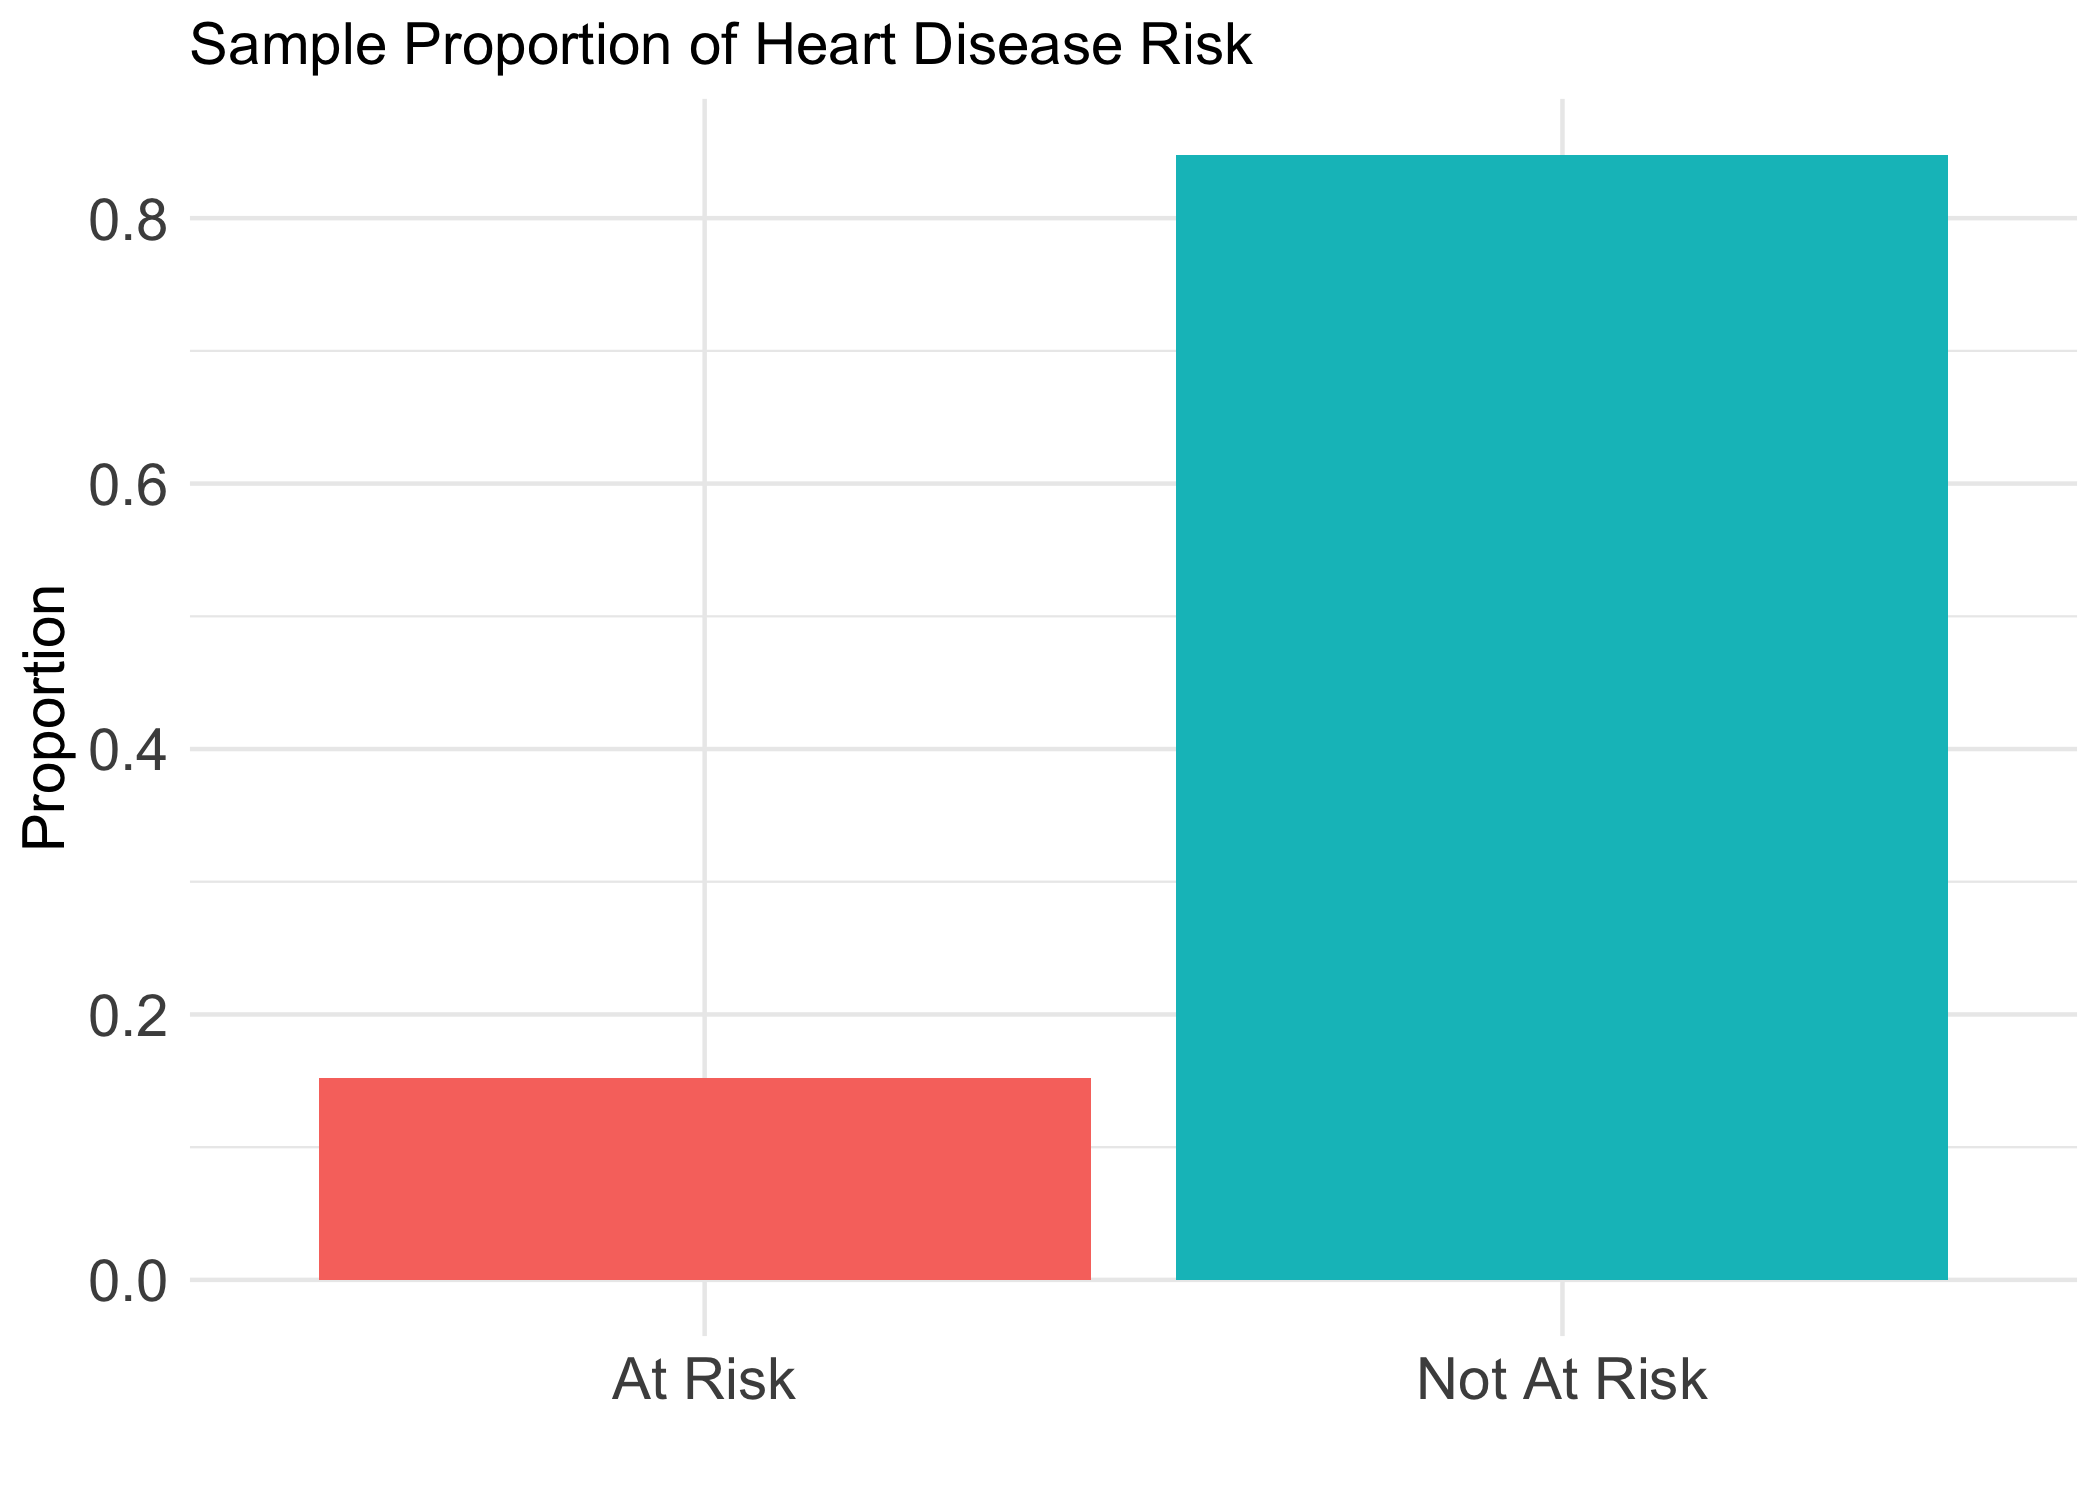
\includegraphics[height=45mm, width=65mm]{bar_chd.png}
\end{figure}

\subsubsection*{Sex}

In our study, 55\% of the patients are female and 45\% of patients are male. According to the two-way proportions plot below, we see that males are slightly more likely to have heart disease compared to the females in this study. 

\begin{figure}[ht!]
\hspace*{\fill}
\centering
\subcaptionbox*{}{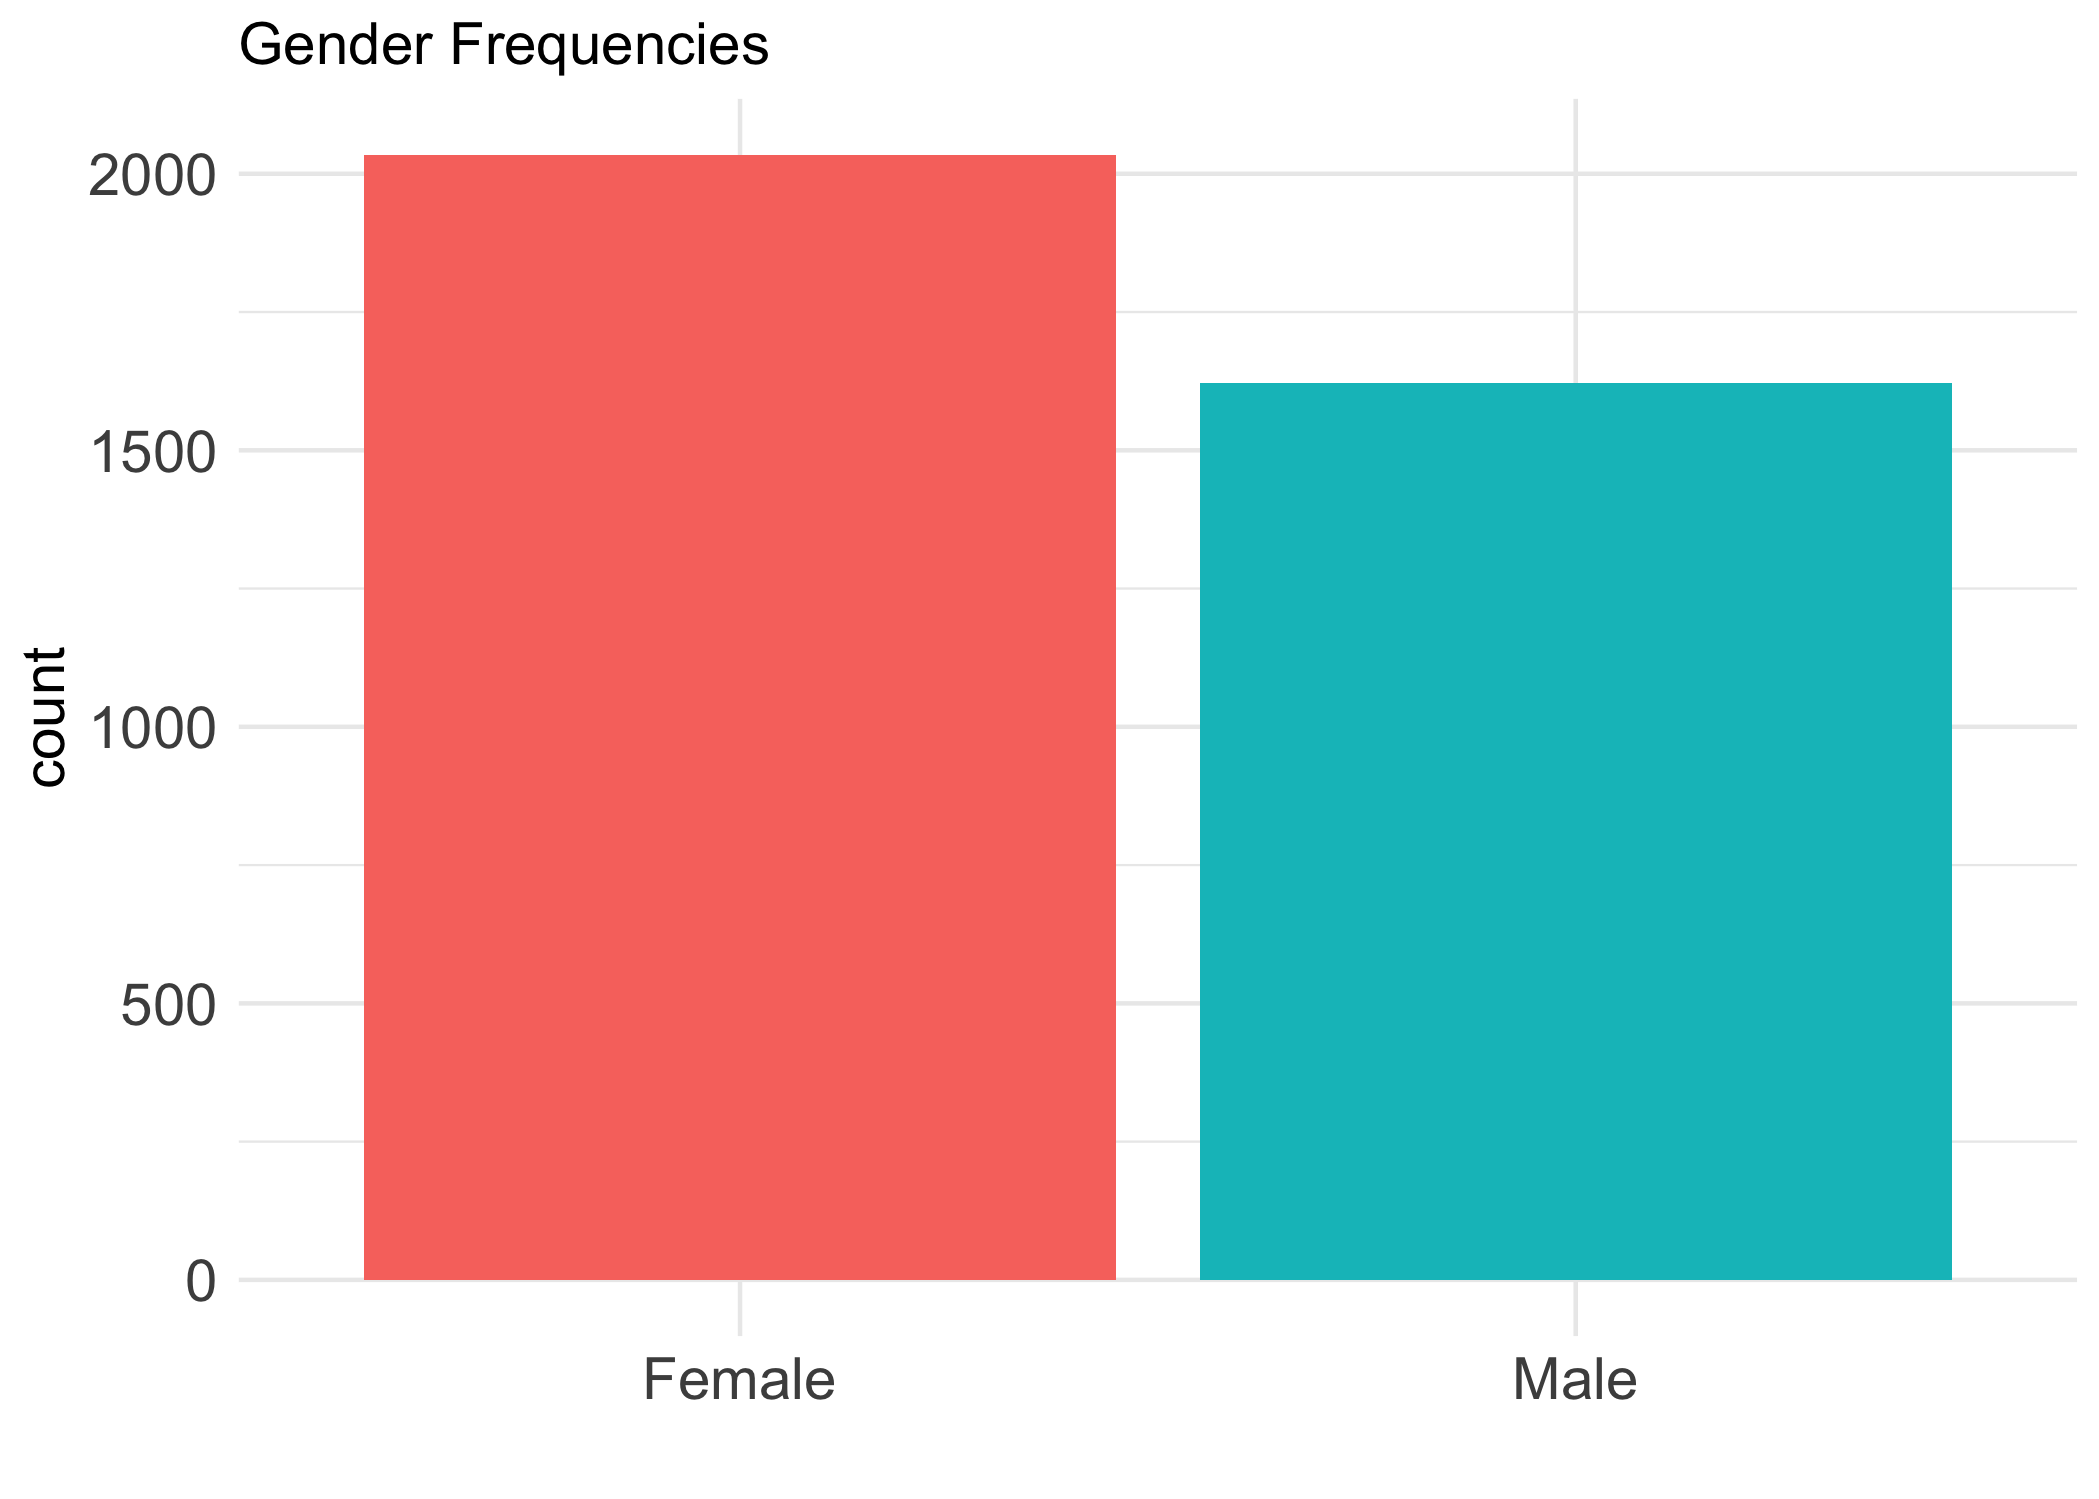
\includegraphics[height=45mm, width=65mm]{bar_sex.png}}\hspace{2em}%
\subcaptionbox*{}{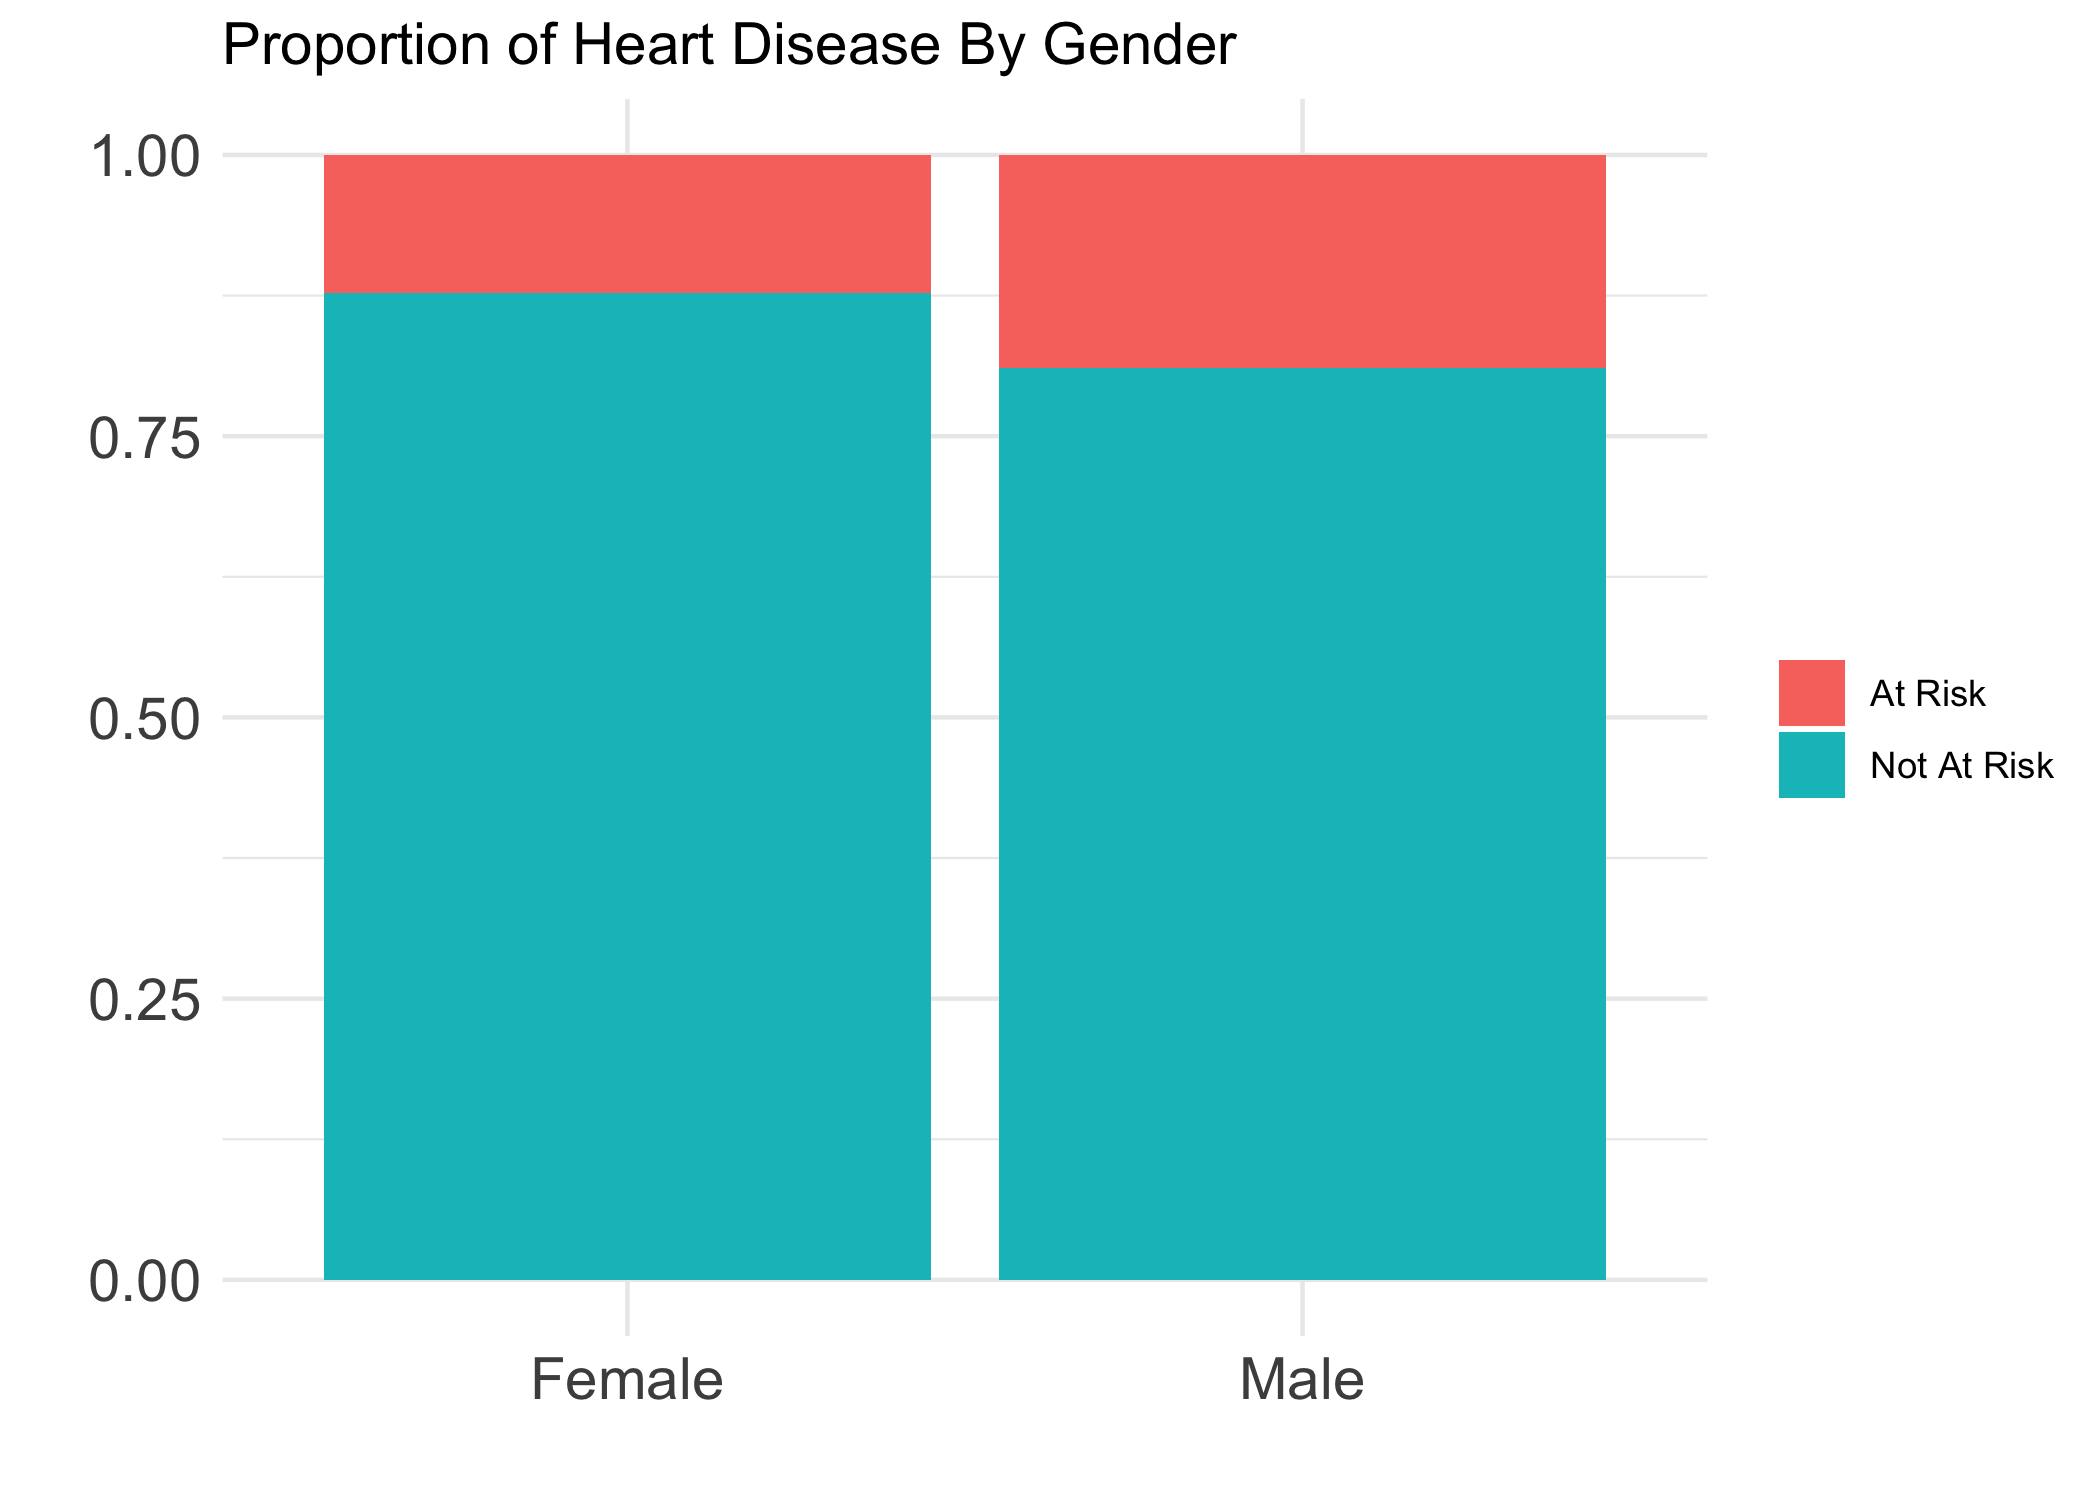
\includegraphics[height=45mm, width=65mm]{two_way_sex.png}}%
\hspace*{\fill}
\end{figure}

\subsubsection*{Age}

The most common age groups in the data are patients in their 40's and 50's. We can see that older patients' are generally associated with more heart disease risk.

\begin{figure}[ht!]
\hspace*{\fill}
\centering
\subcaptionbox*{}{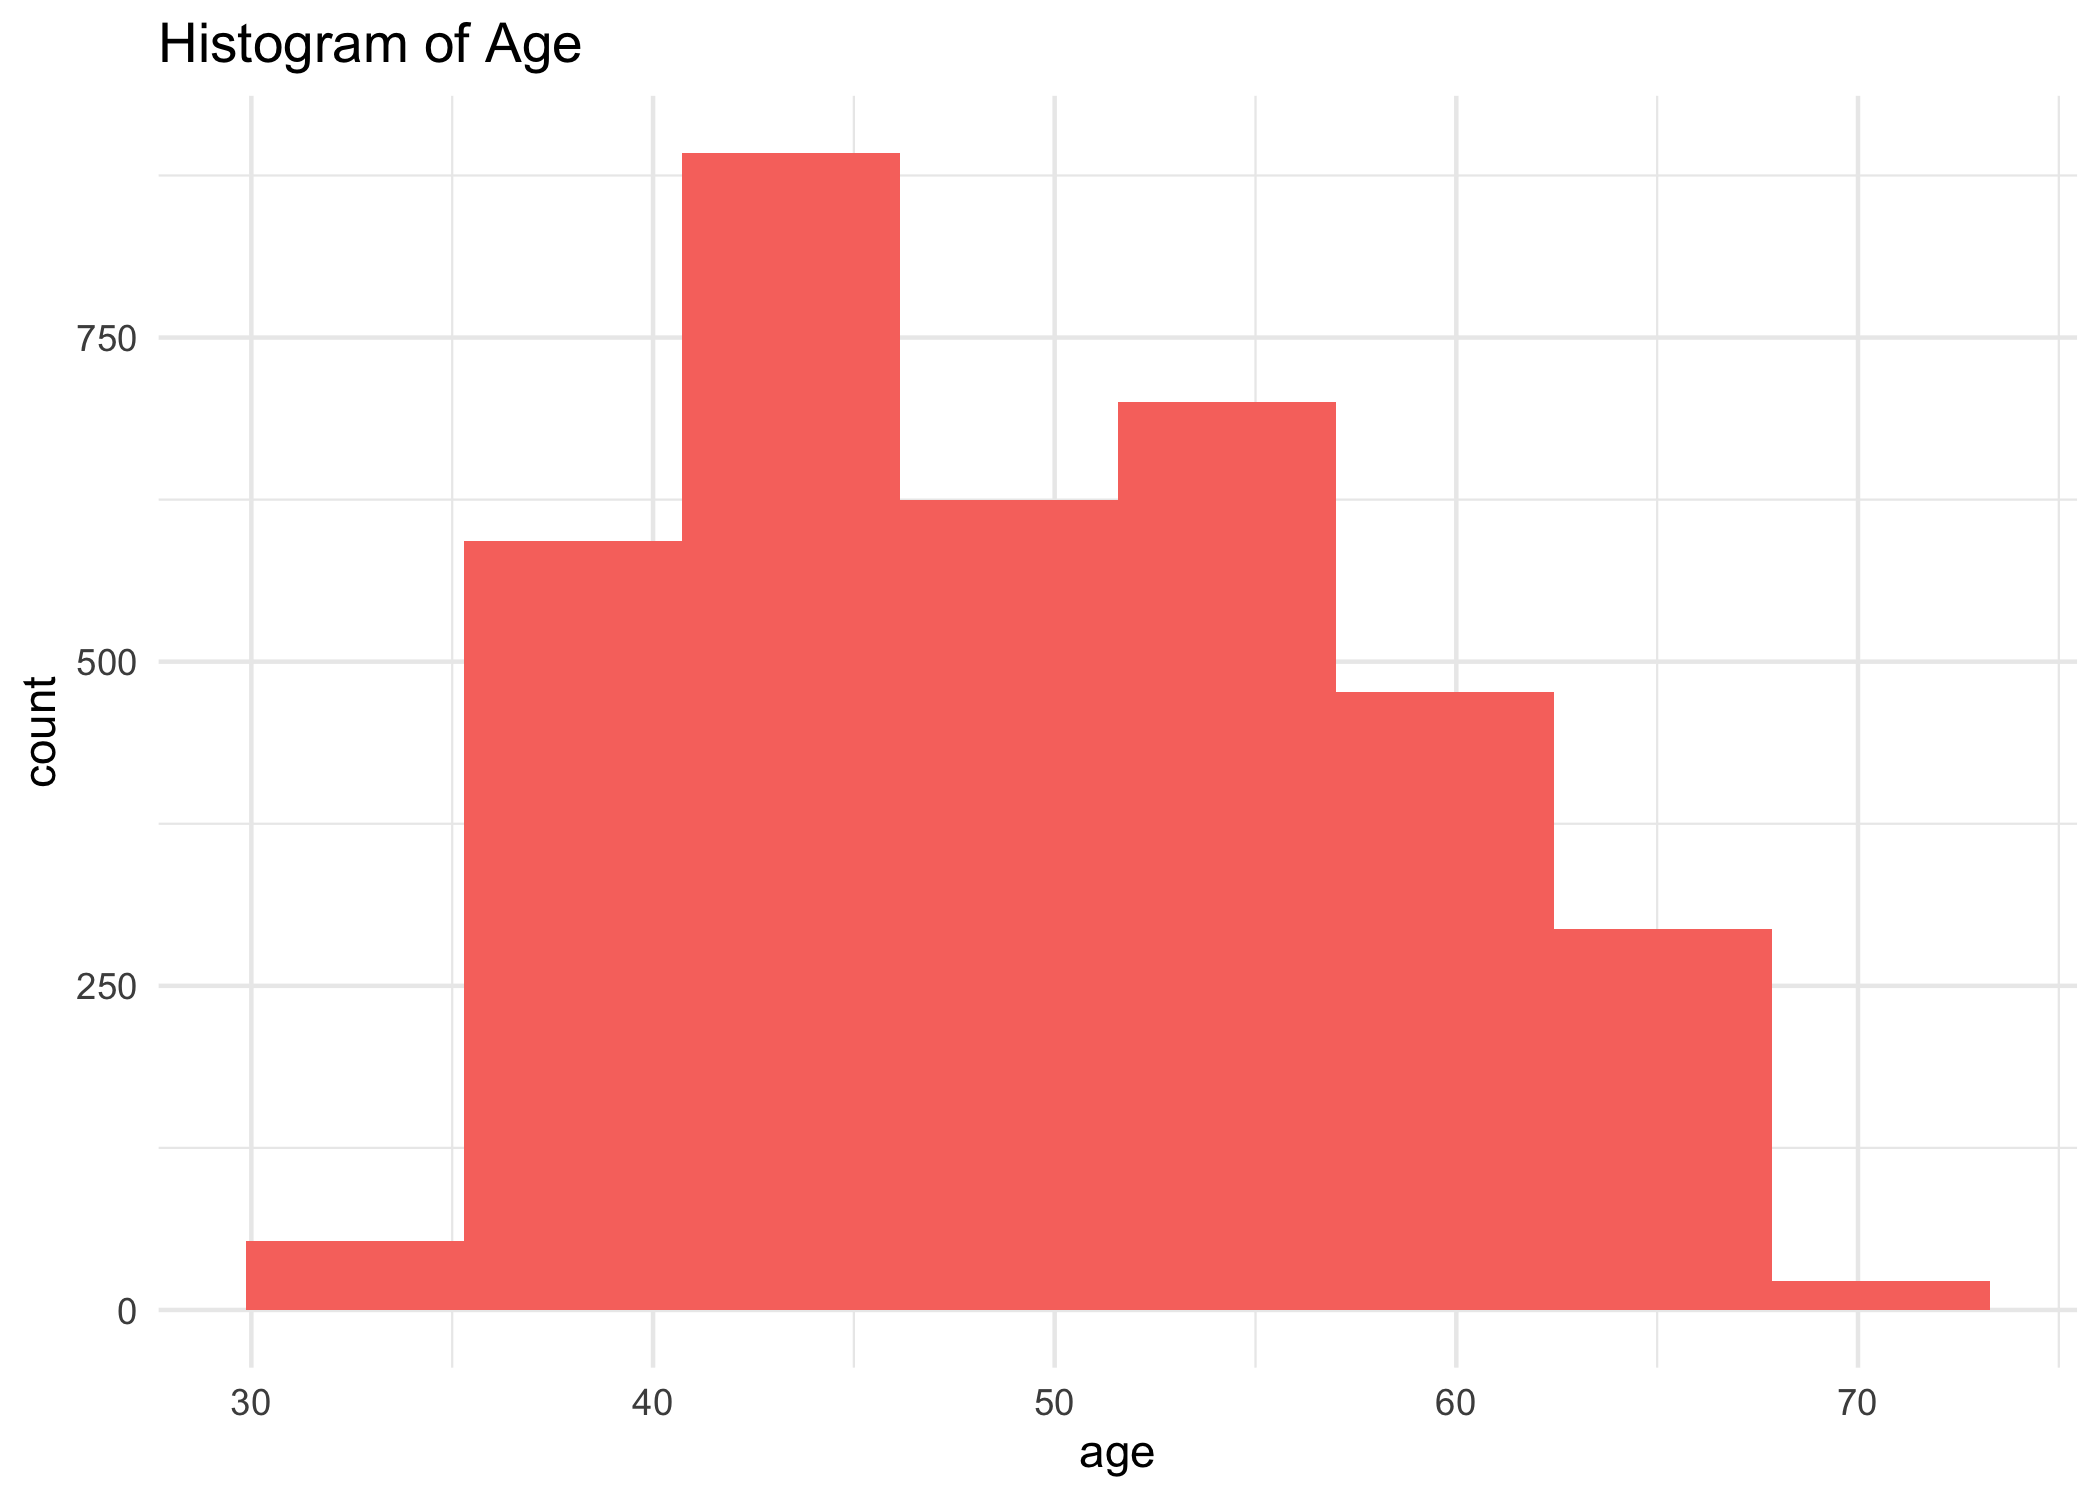
\includegraphics[height=45mm, width=65mm]{hist_age.png}}\hspace{2em}%
\subcaptionbox*{}{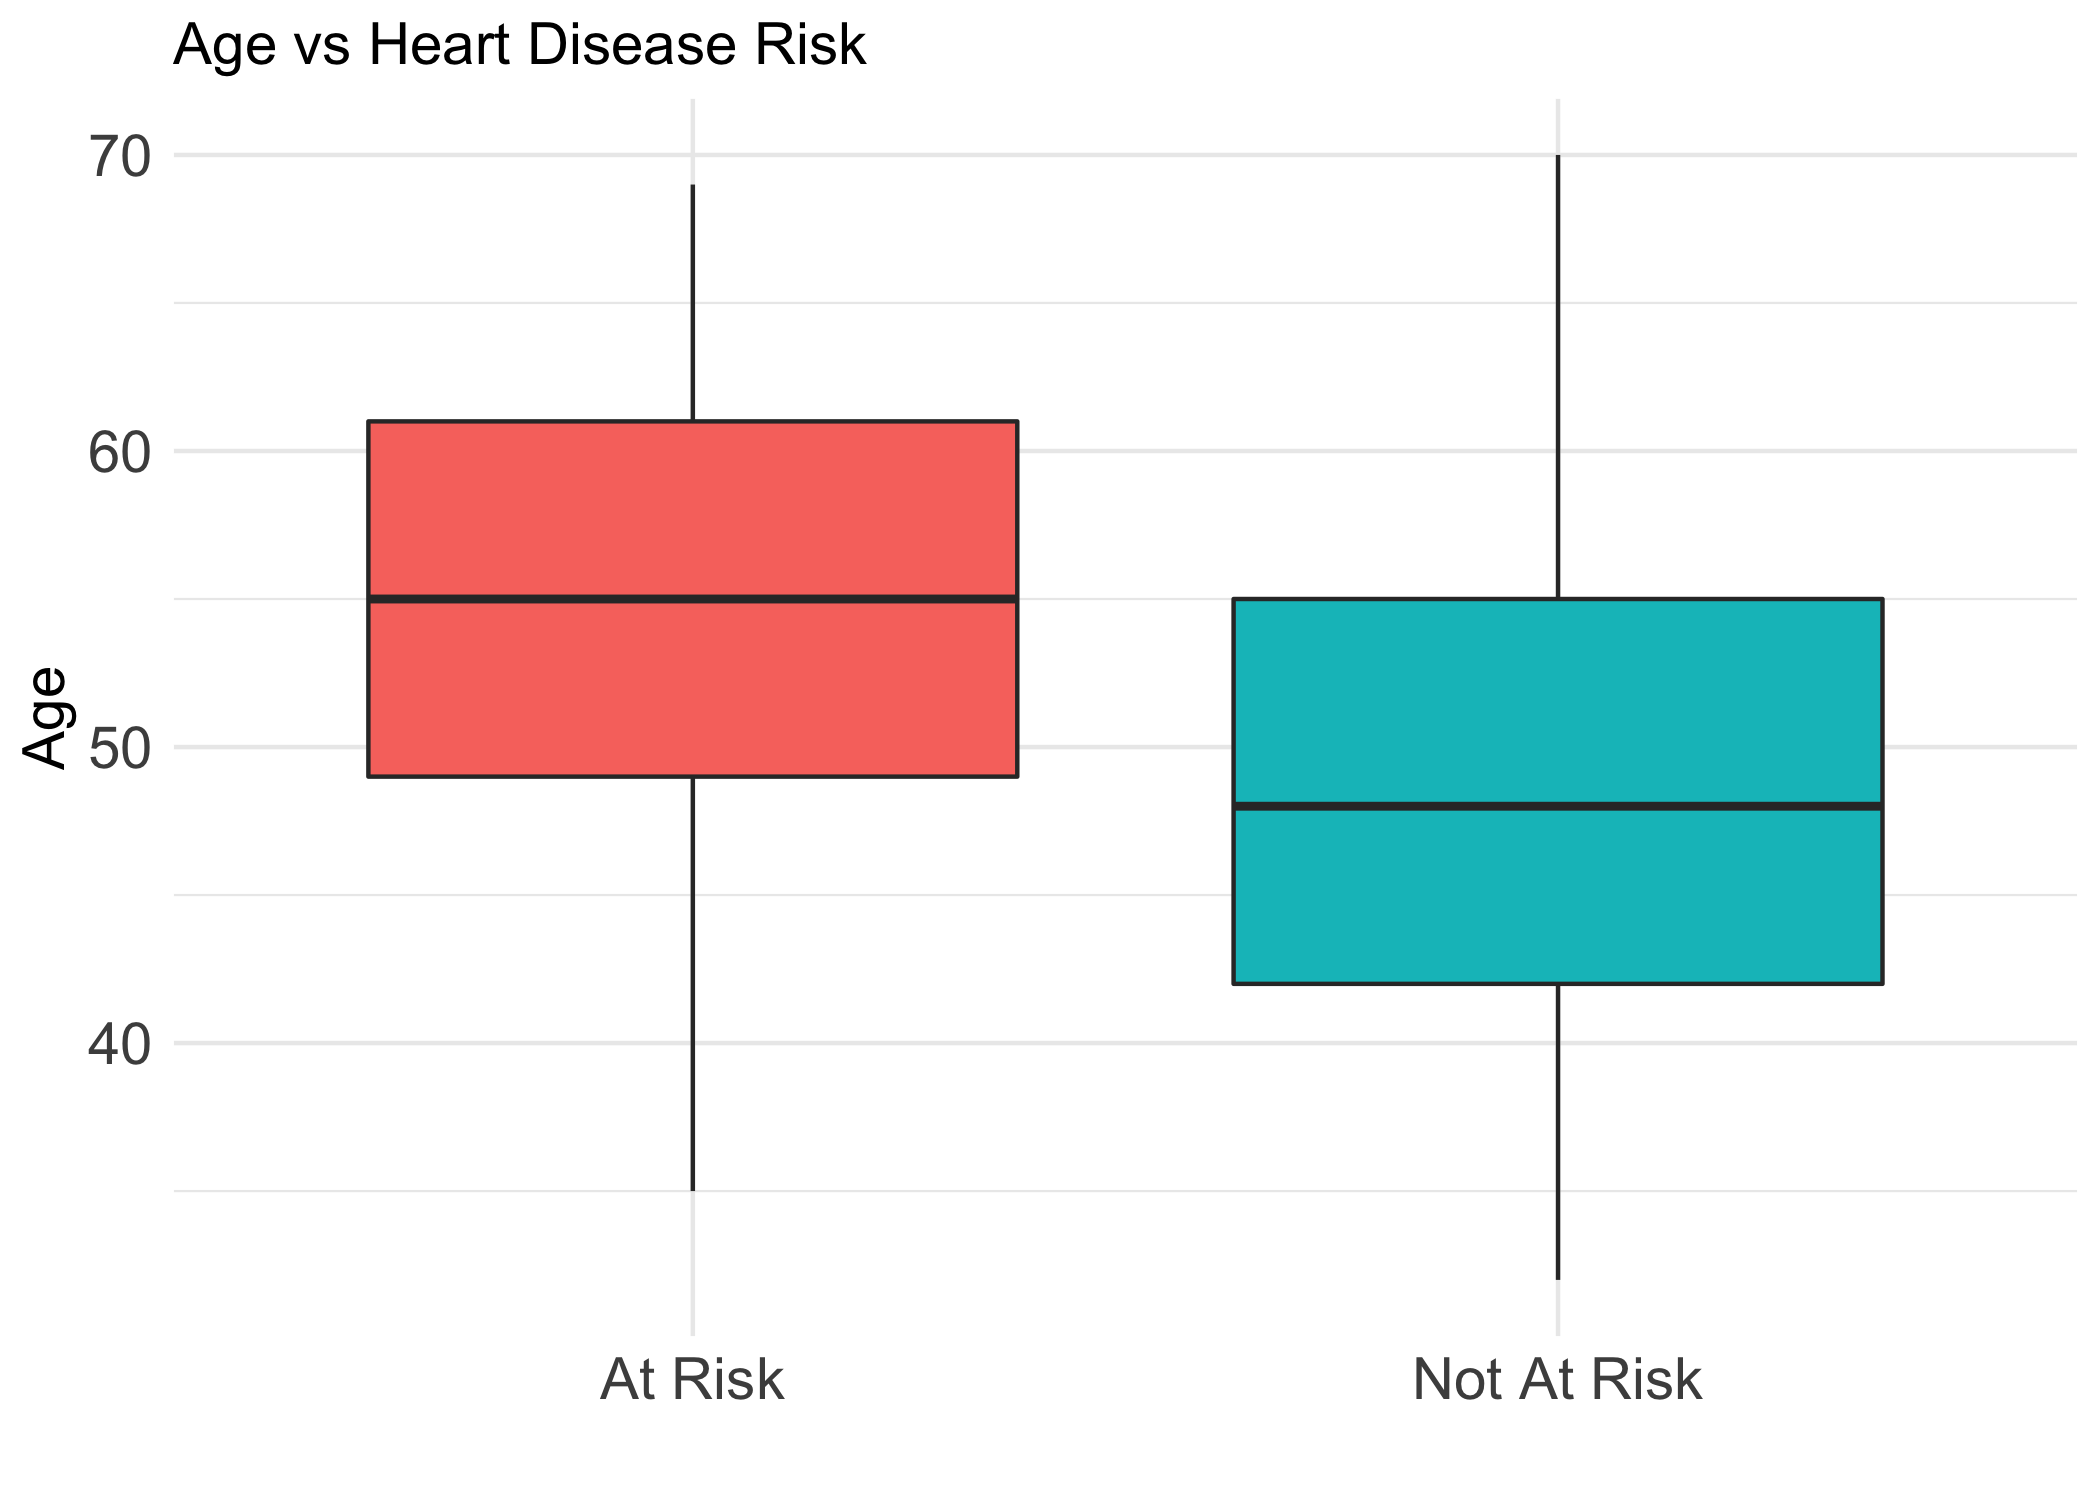
\includegraphics[height=45mm, width=65mm]{box_age.png}}%
\hspace*{\fill}
\end{figure}



\subsubsection*{Education}

According to the plot below, nearly half of the patients do not have a high school education while one-third of patients have a bachelor's degree or a graduate school degree. The risk of 10-year coronary heart disease among patients with at least a high school education appears less than the proportion of heart disease among patients with less than a high school education.

\begin{figure}[hbt!]
\hspace*{\fill}
\centering
\subcaptionbox*{}{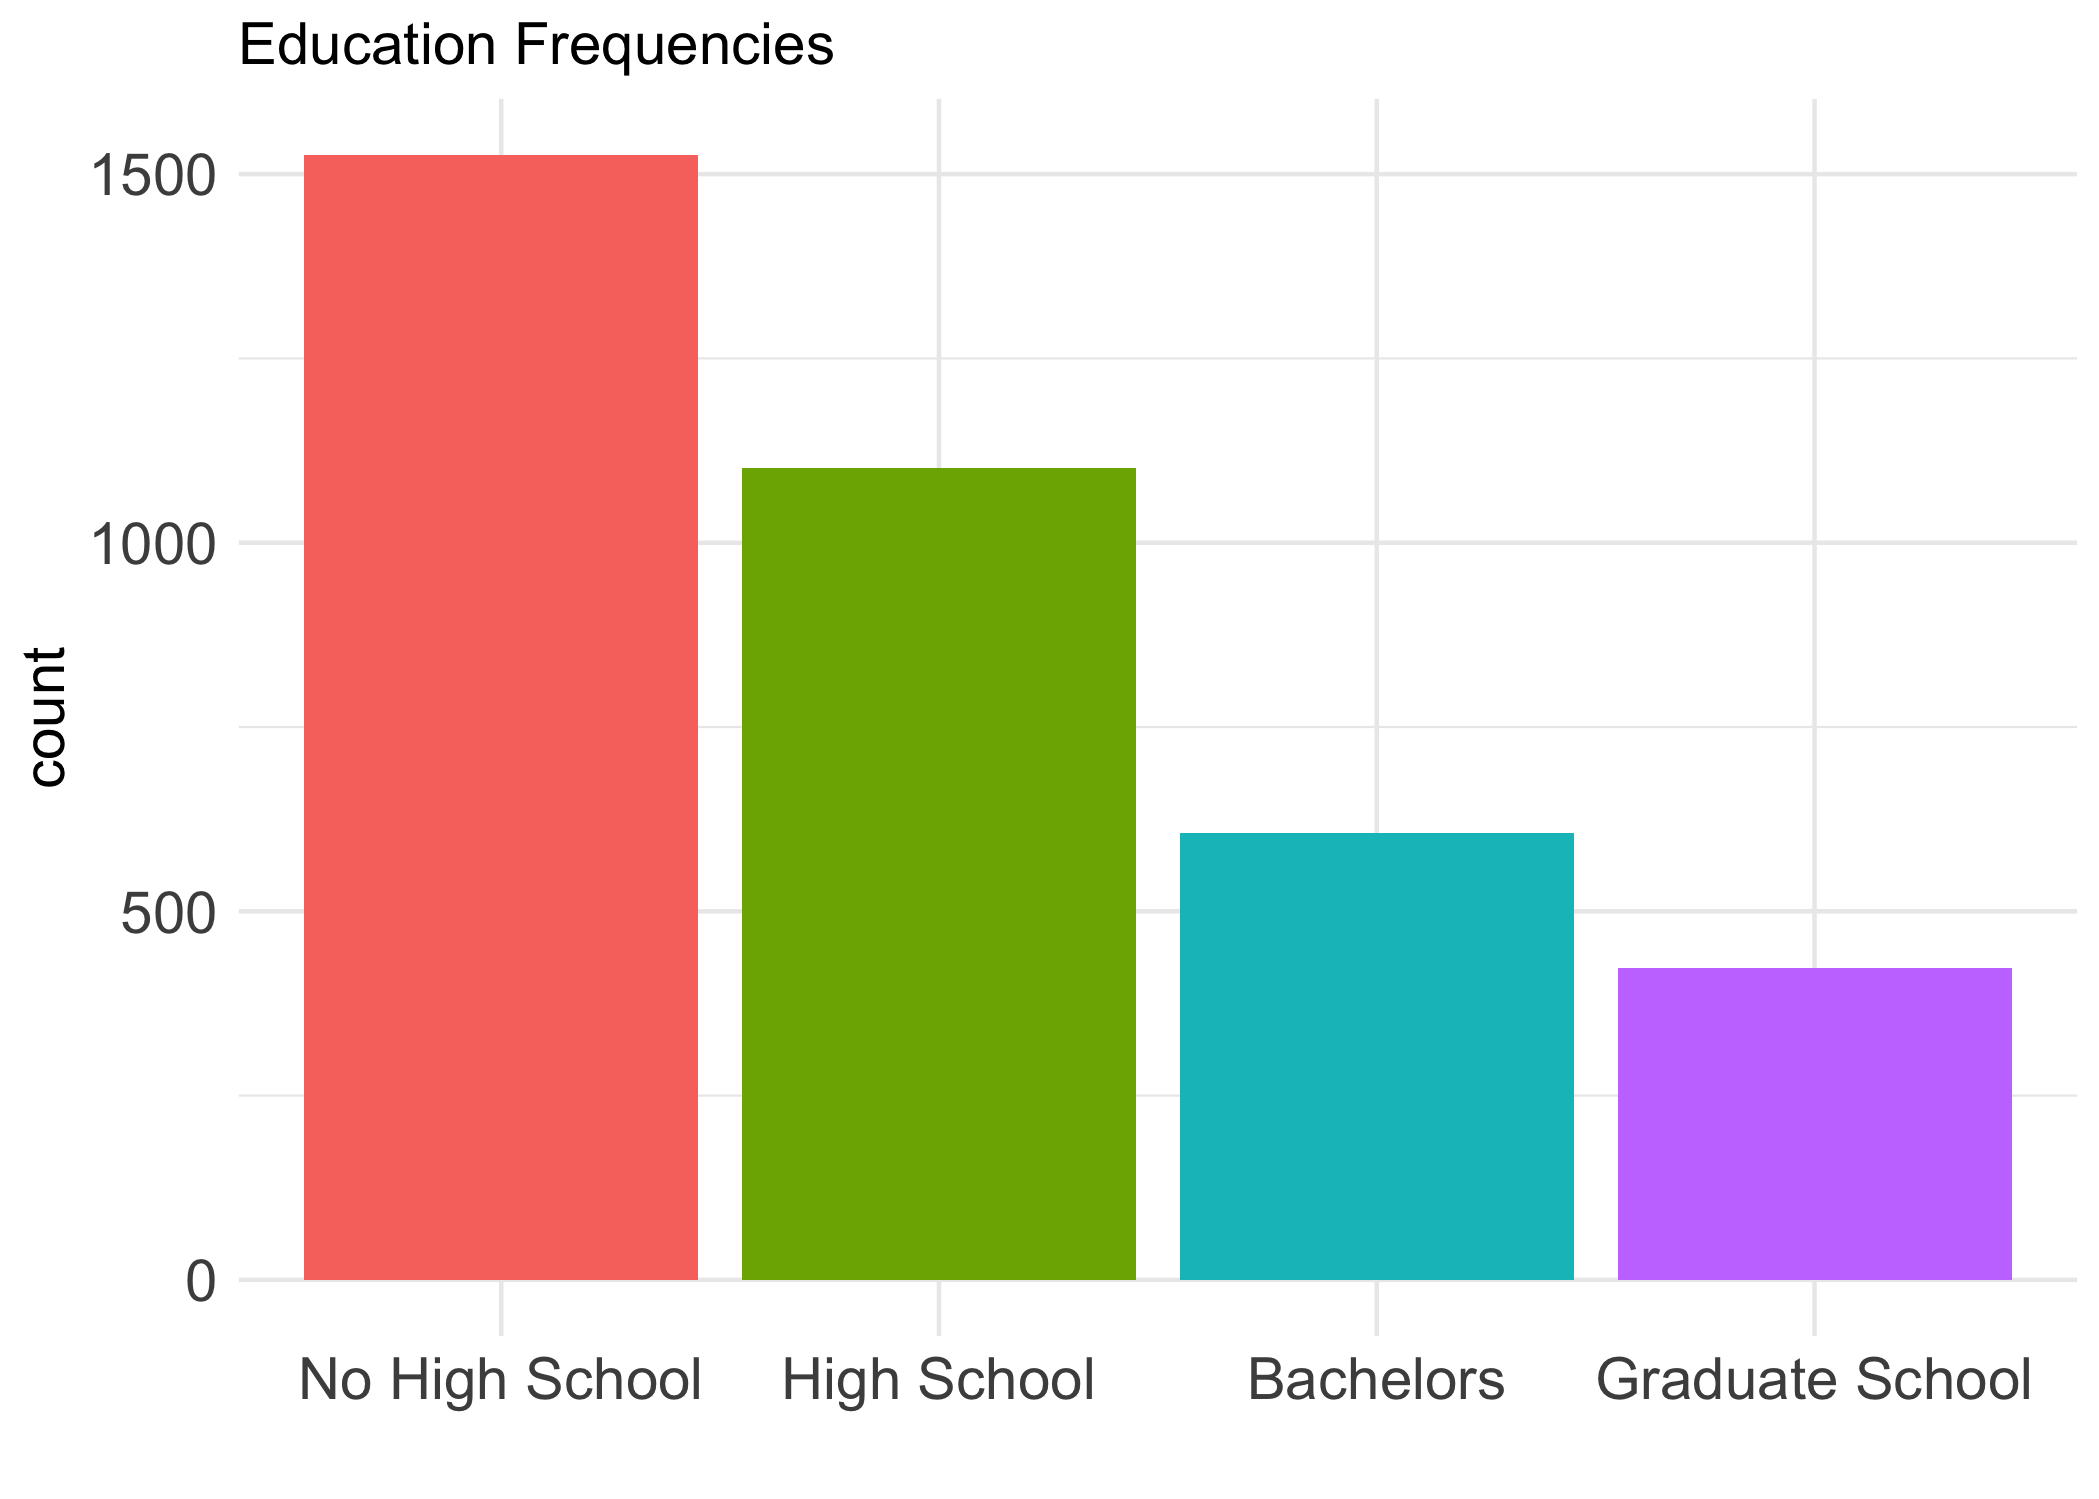
\includegraphics[height=45mm, width=65mm]{bar_education.png}}\hspace{2em}%
\subcaptionbox*{}{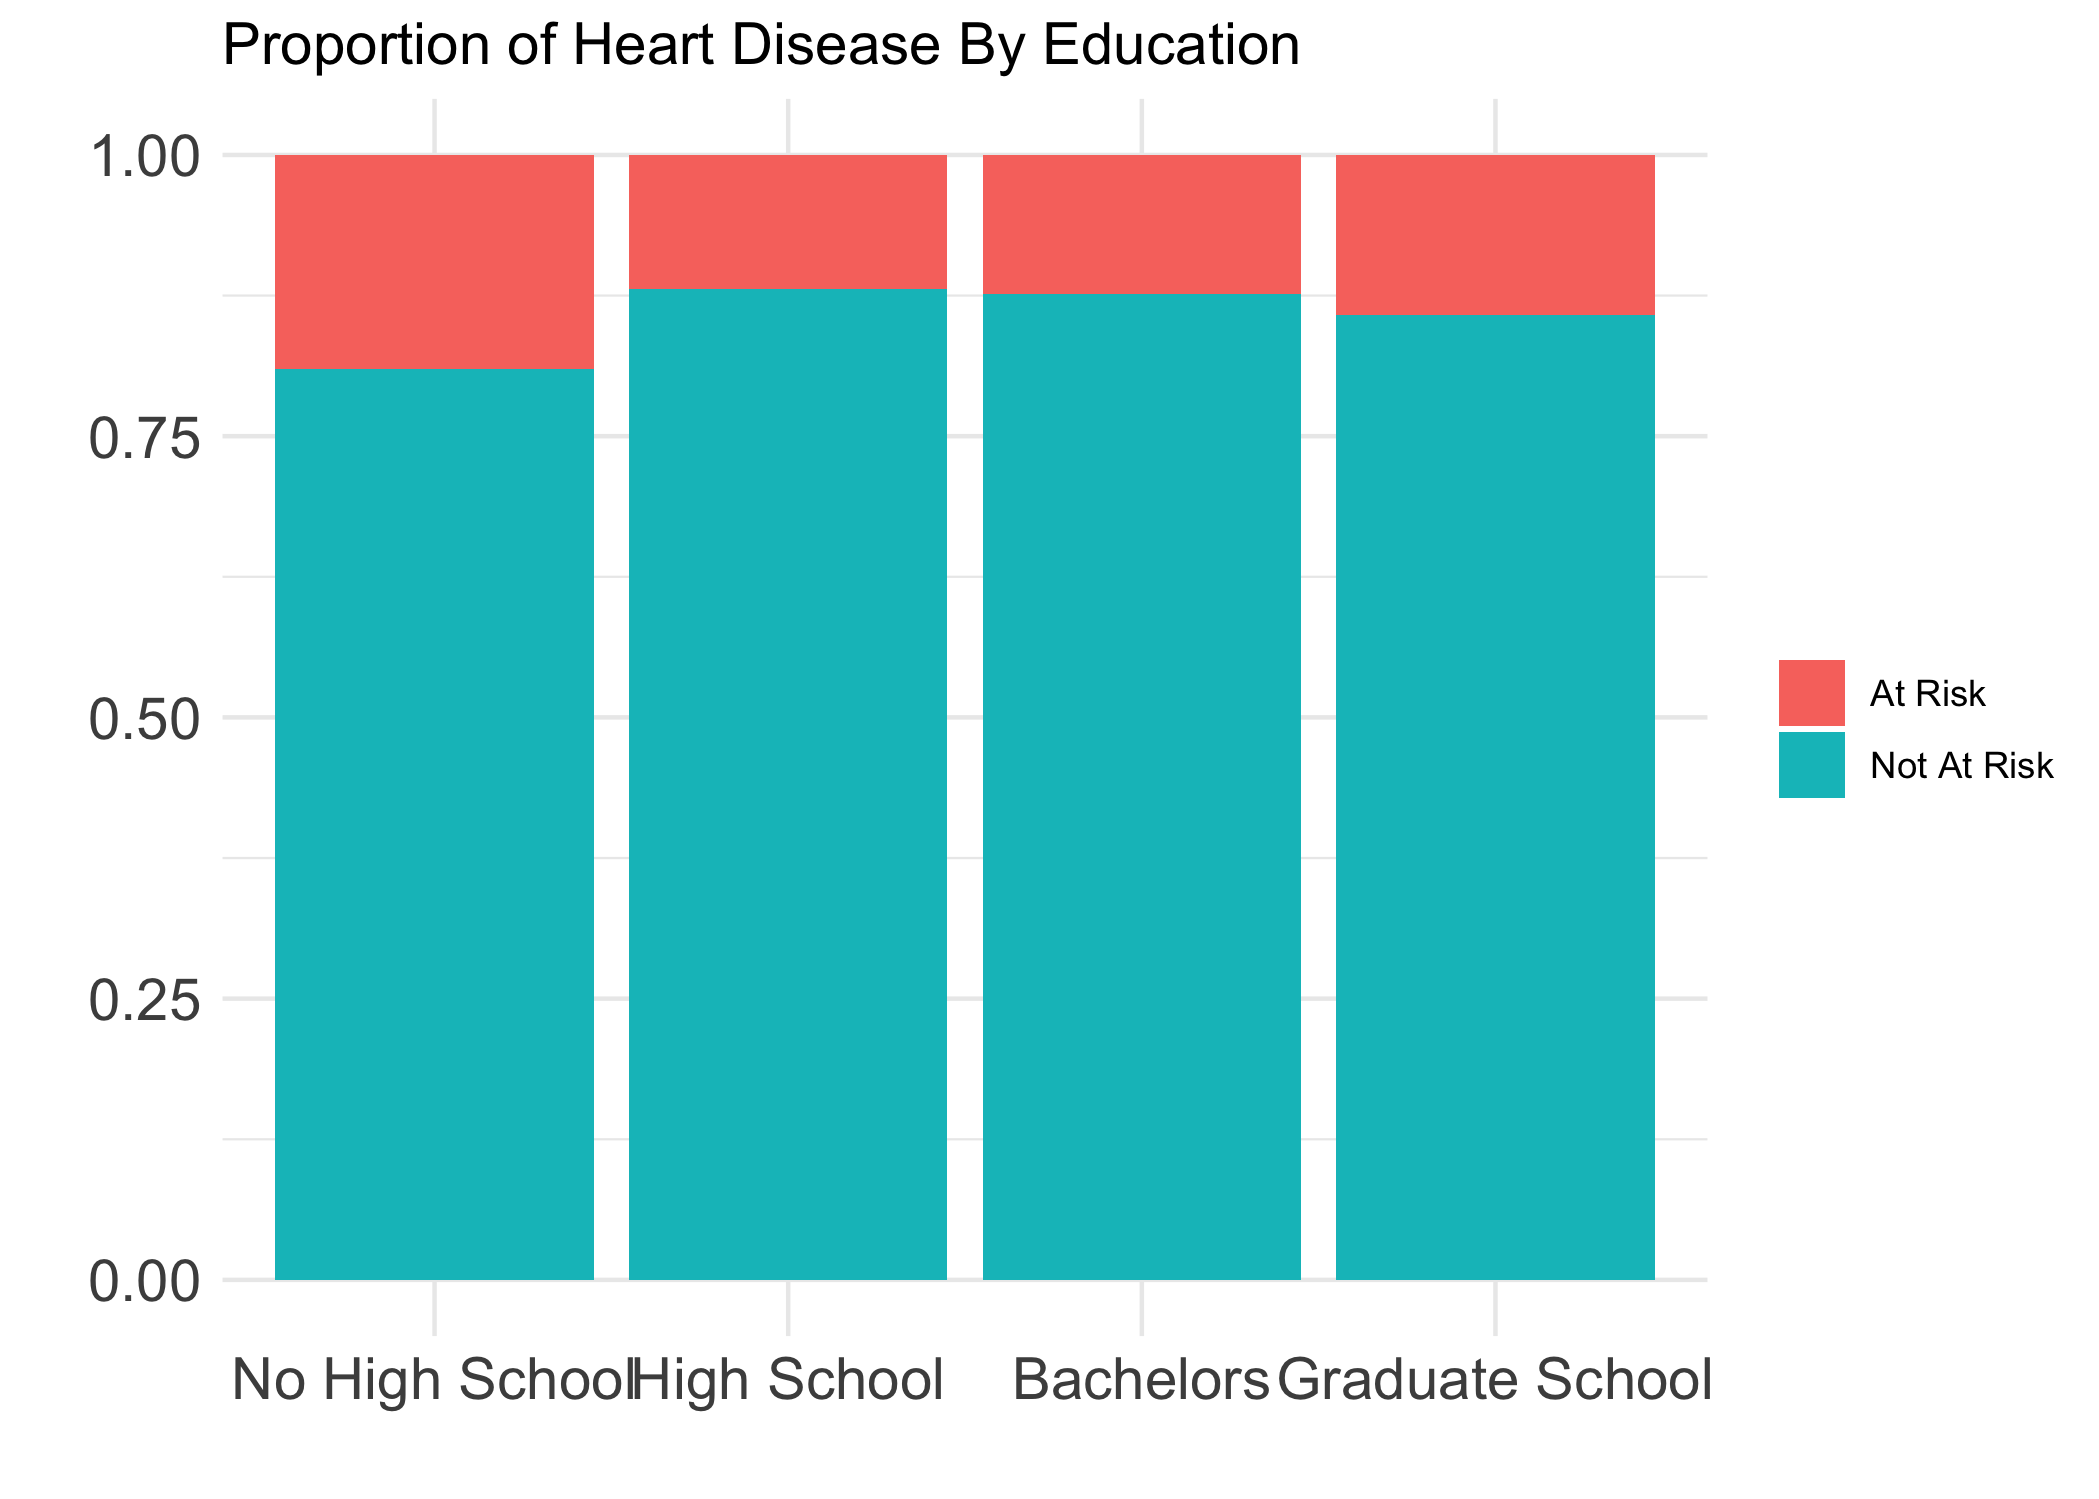
\includegraphics[height=45mm, width=65mm]{two_way_education.png}}%
\hspace*{\fill}
\end{figure}



\subsubsection*{Smoker Status}

In our dataset, the number of smokers is nearly equivalent to non-smokers. Surprisingly, the risk of 10-year coronary heart disease across both groups is approximately equal. Typically, we would expect smokers to have a slightly larger risk of 10-year coronary heart disease.

\begin{figure}[hbt!]
\hspace*{\fill}
\centering
\subcaptionbox*{}{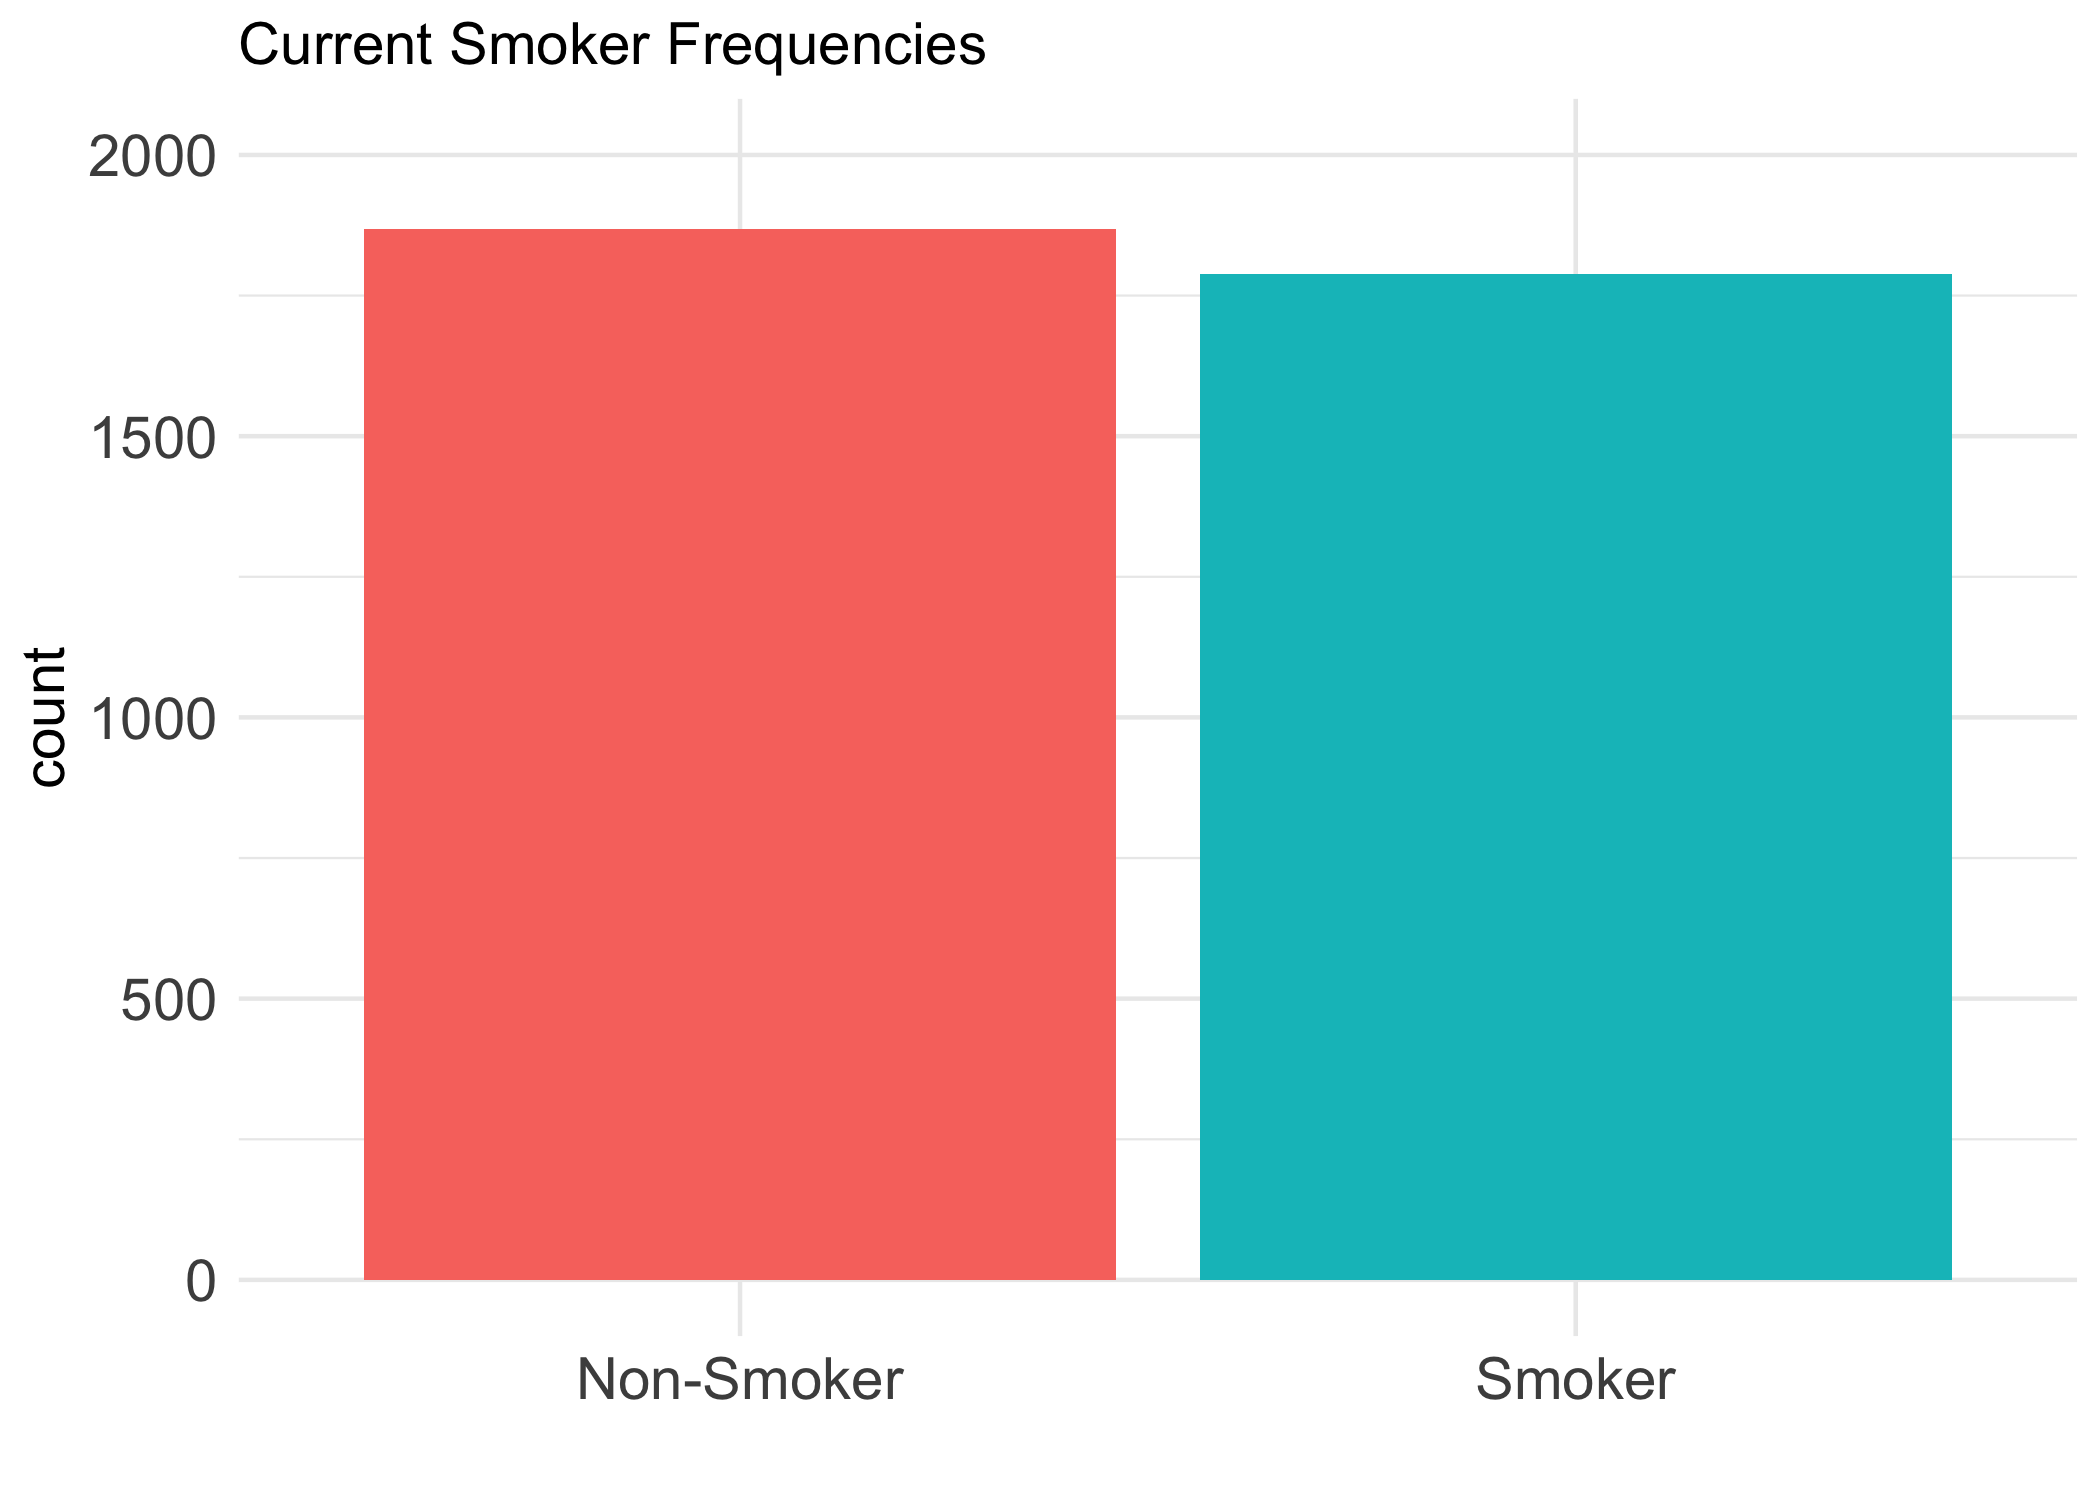
\includegraphics[height=45mm, width=65mm]{bar_smoker_status.png}}\hspace{2em}%
\subcaptionbox*{}{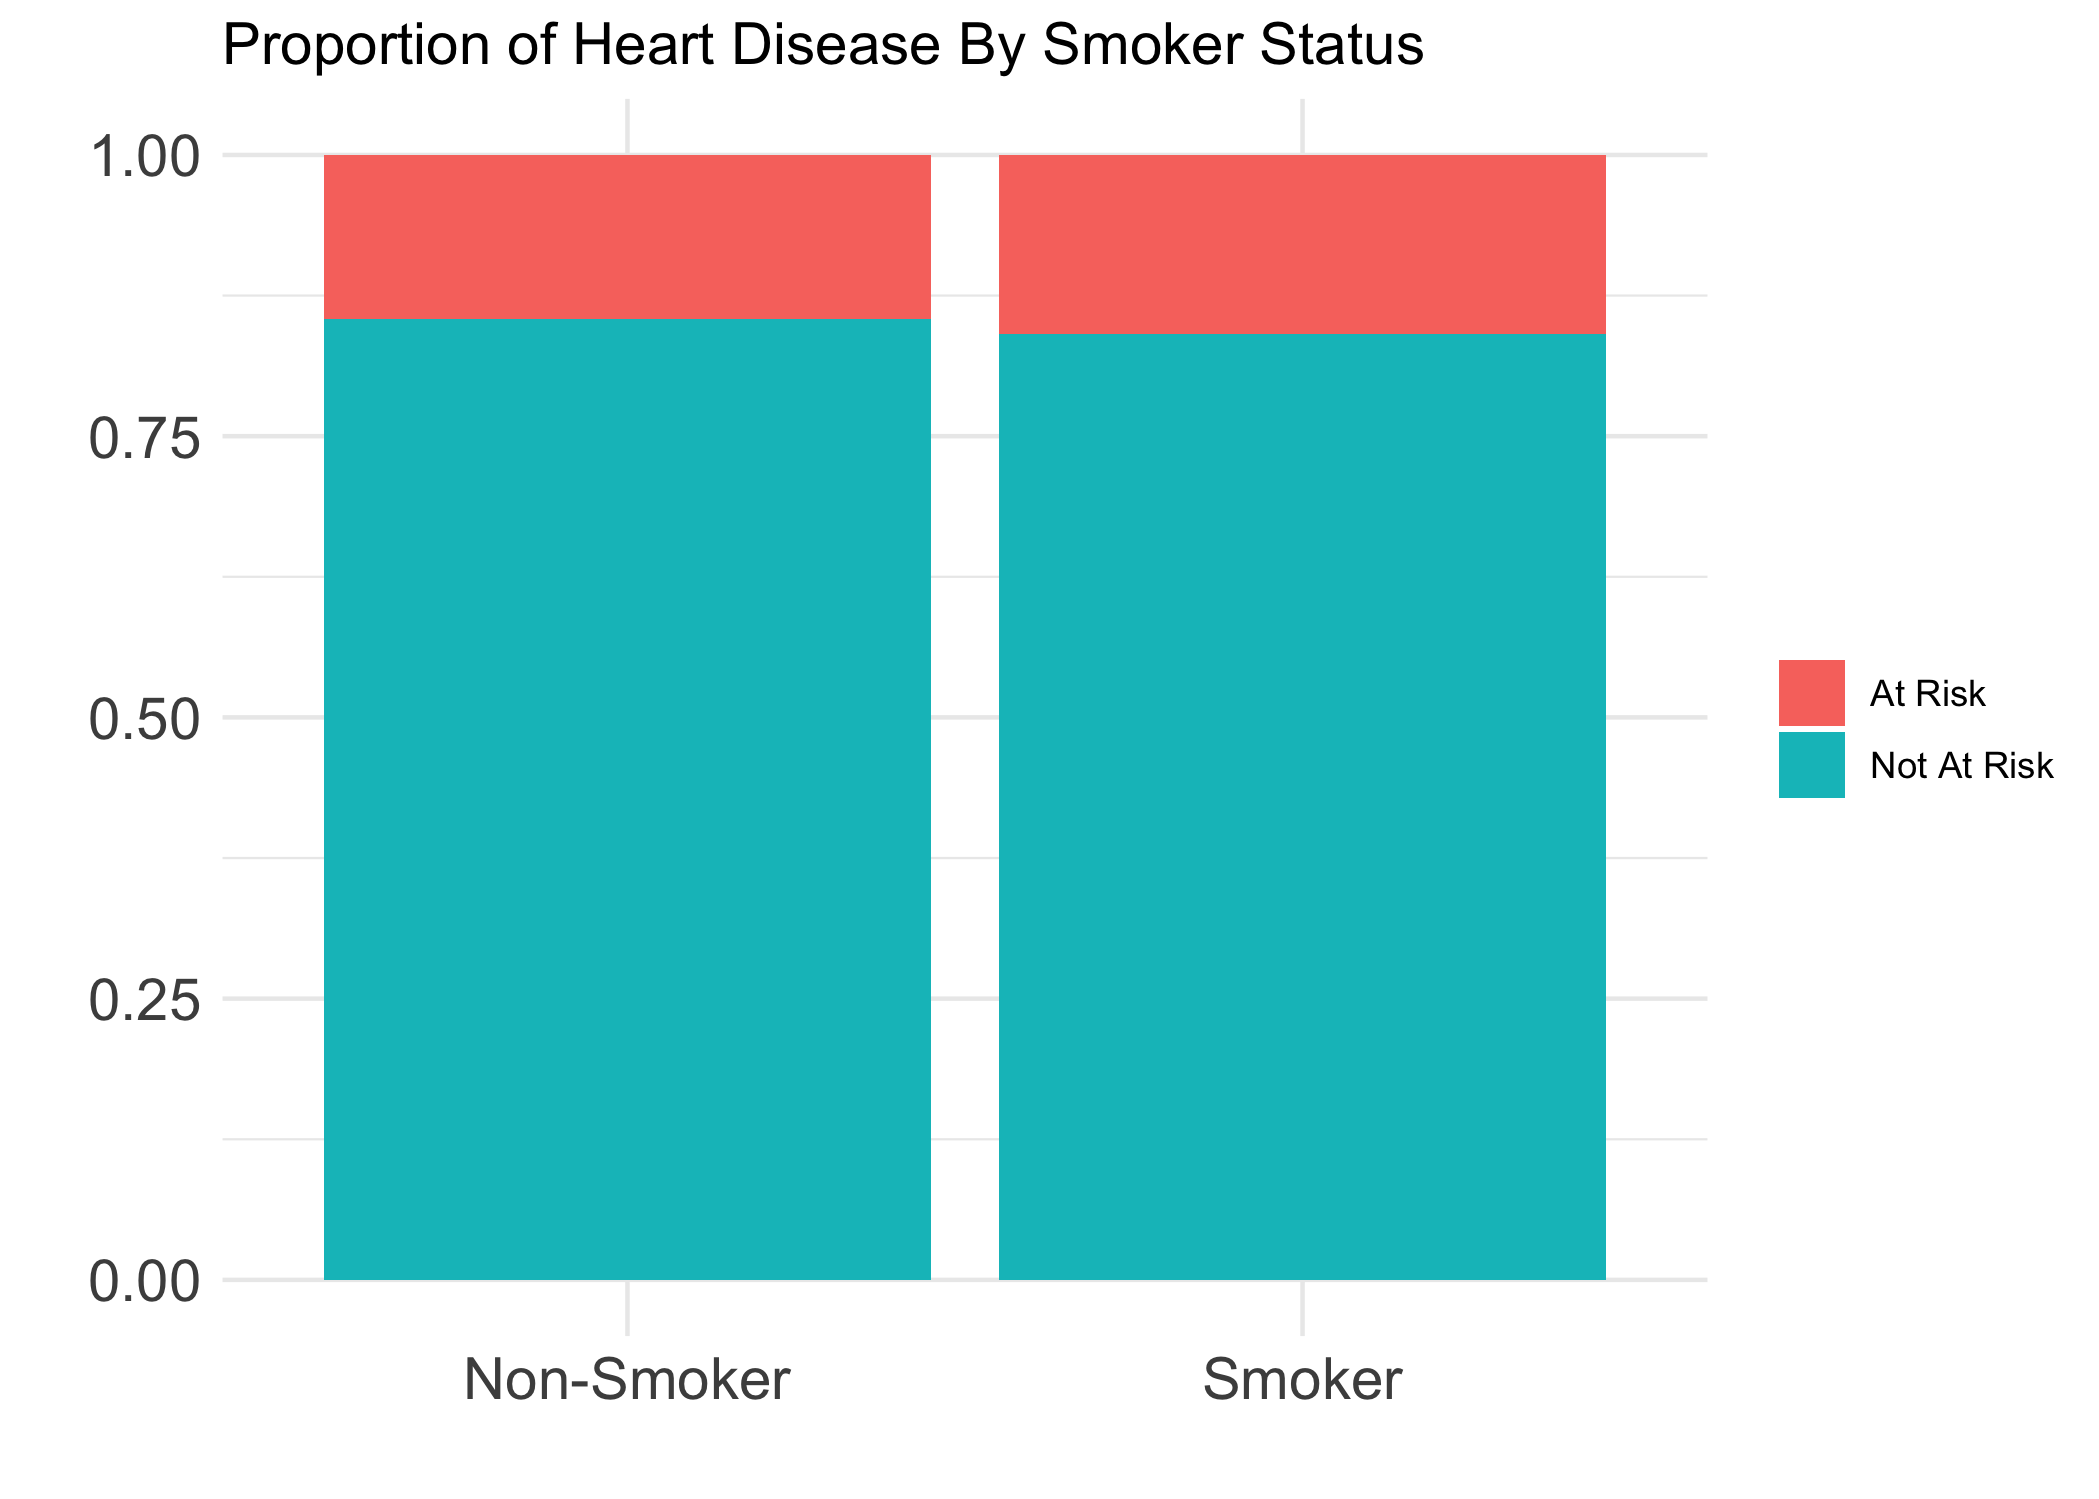
\includegraphics[height=45mm, width=65mm]{two_way_smoker_status.png}}%
\hspace*{\fill}
\end{figure}


\subsubsection*{Cigarettes Smoked Per Day}

As mentioned above, nearly half our dataset consists of non-smokers. But, for those who do smoke, we see that most patients either smoke many cigarettes per day or have a cigarette addiction. As the smoker type increases from light to addiction, we see the risk of 10-year coronary heart disease increases as expected. 

\begin{figure}[hbt!]
\hspace*{\fill}
\centering
\subcaptionbox*{}{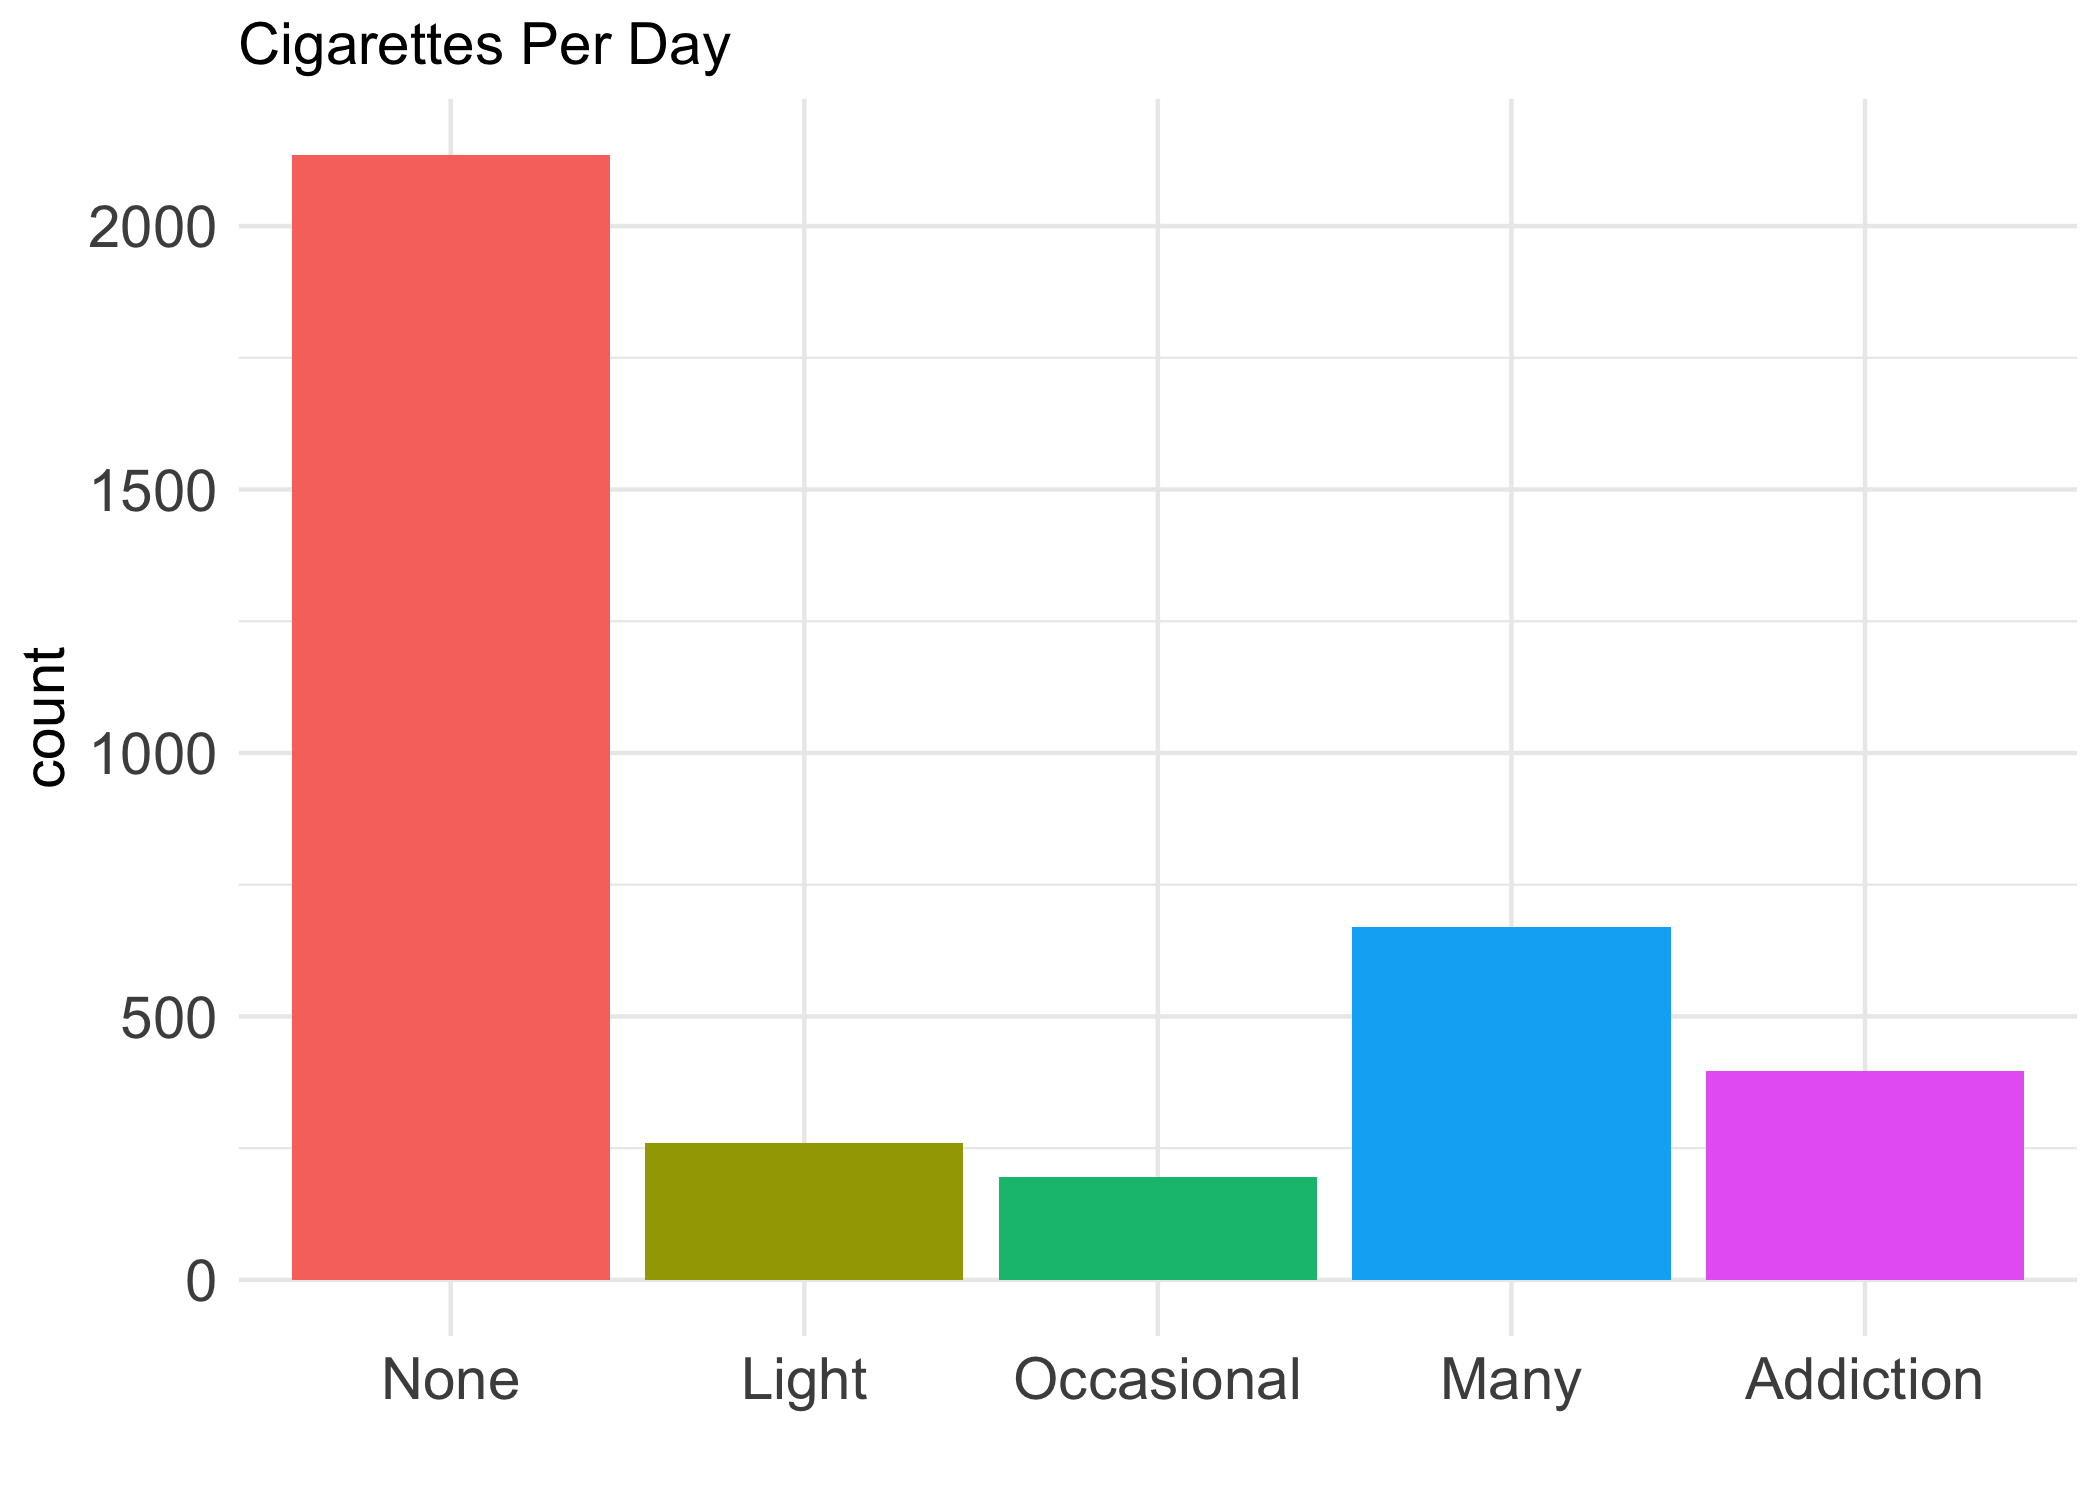
\includegraphics[height=45mm, width=65mm]{bar_cigs_per_day.png}}\hspace{2em}%
\subcaptionbox*{}{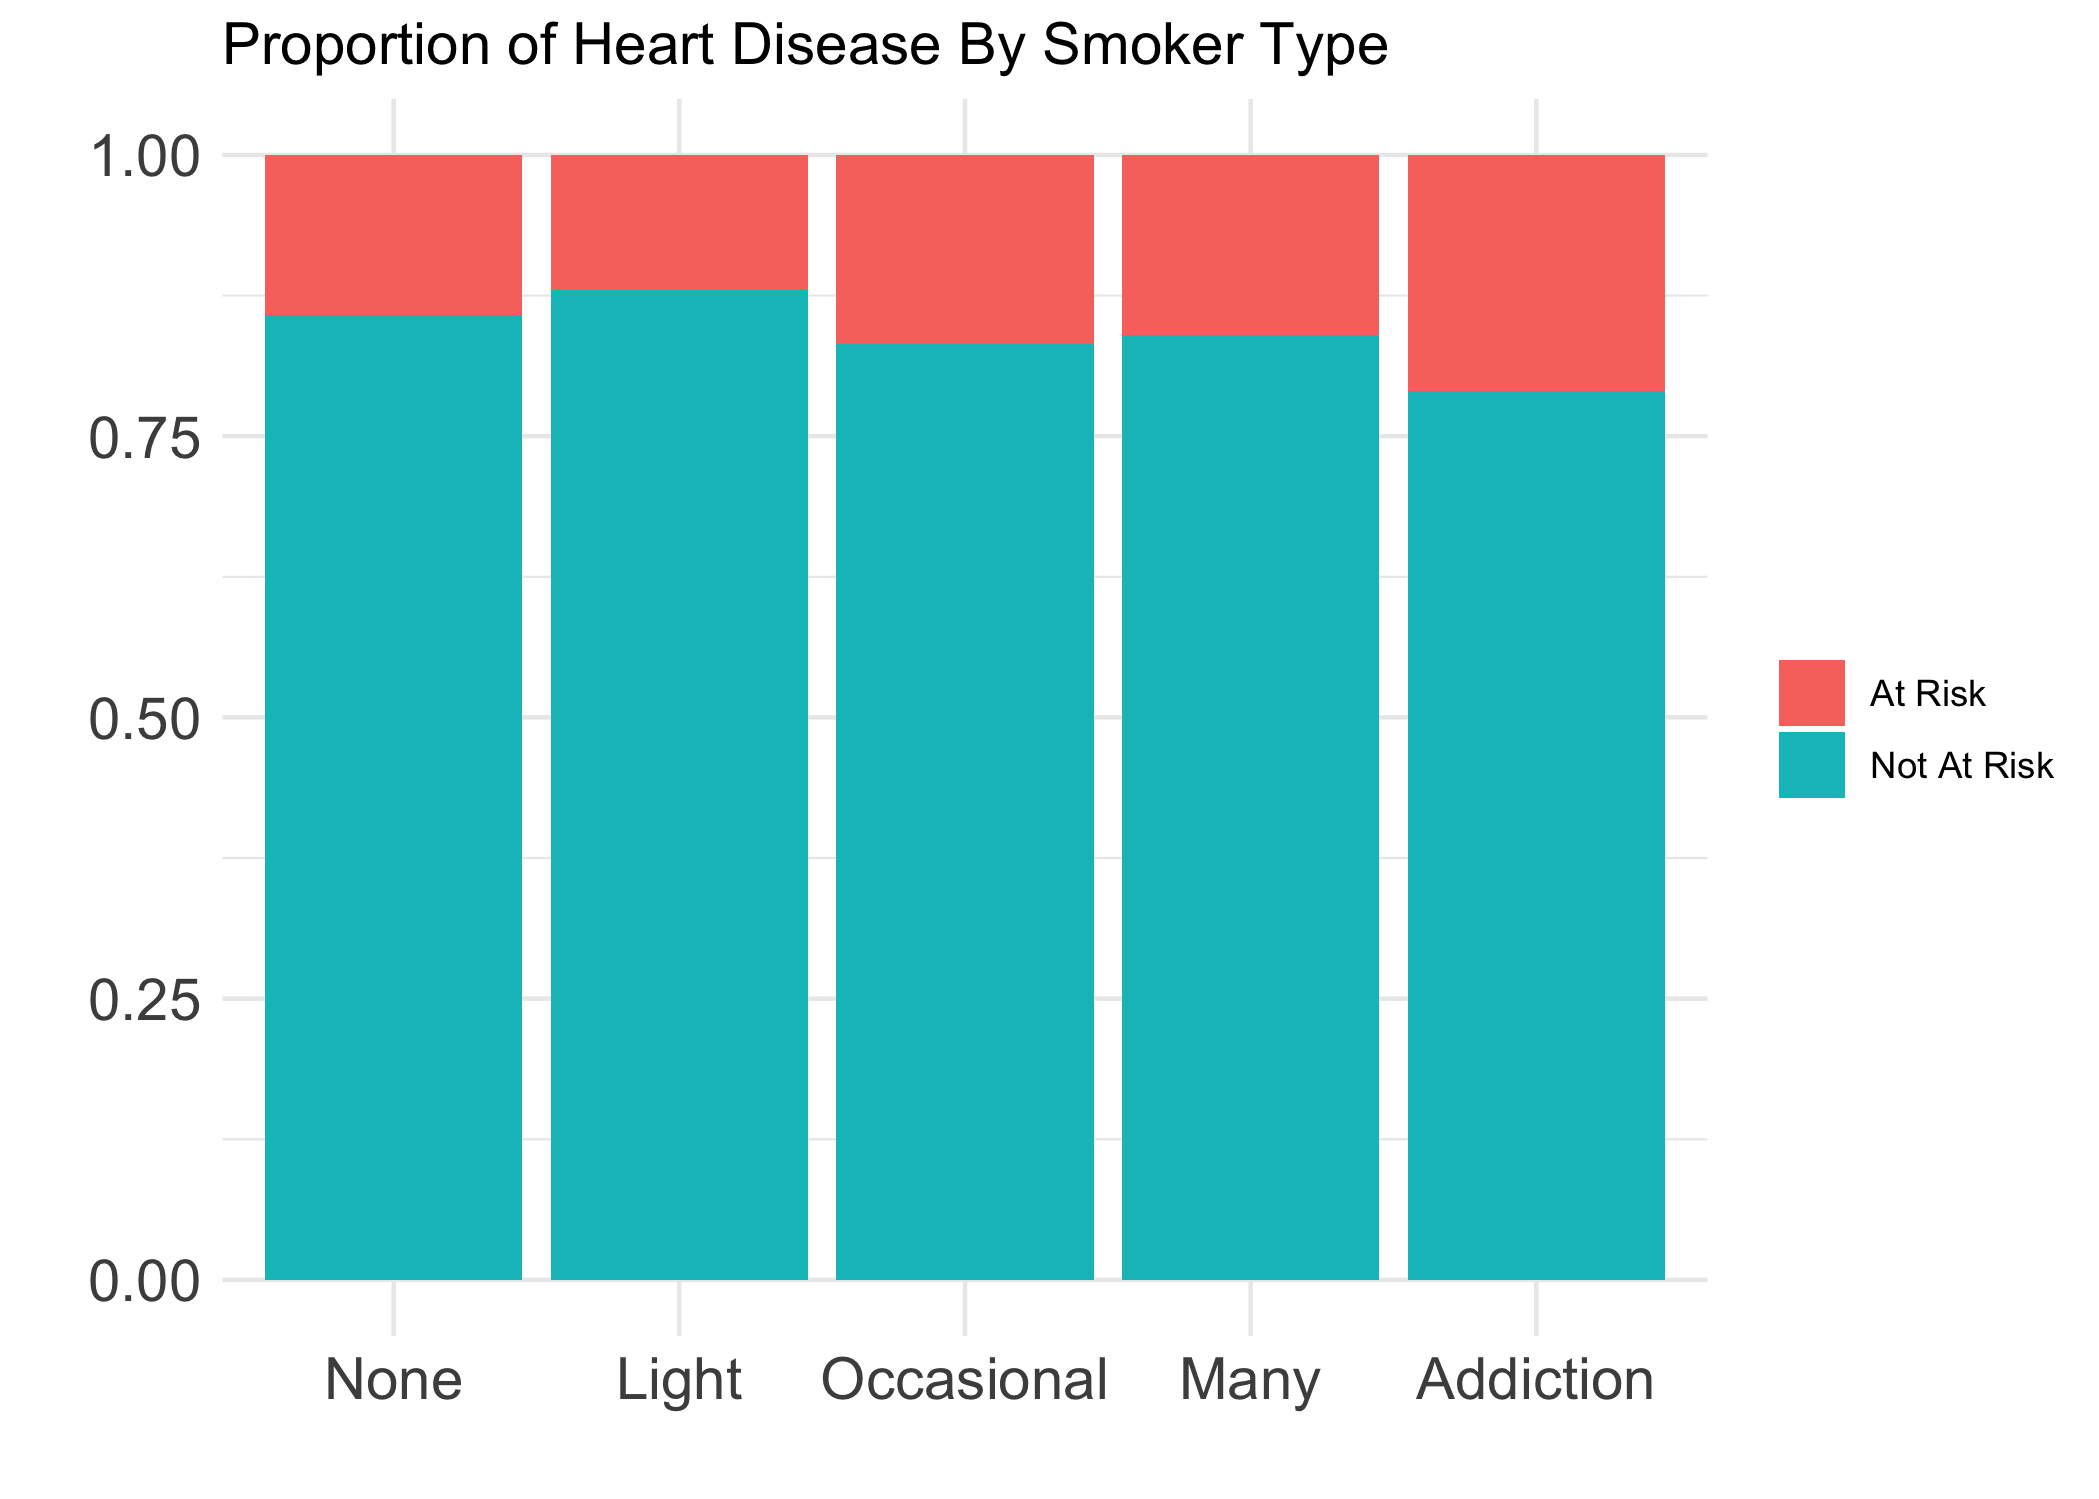
\includegraphics[height=45mm, width=65mm]{two_way_cigs_per_day.png}}%
\hspace*{\fill}
\end{figure}


\subsubsection*{Blood Pressure Medication}

The majority of patients in the study are not on blood pressure medication. For patients on blood pressure medication, over 25\% of patients are at risk for 10-year coronary heart disease.

\begin{figure}[hbt!]
\hspace*{\fill}
\centering
\subcaptionbox*{}{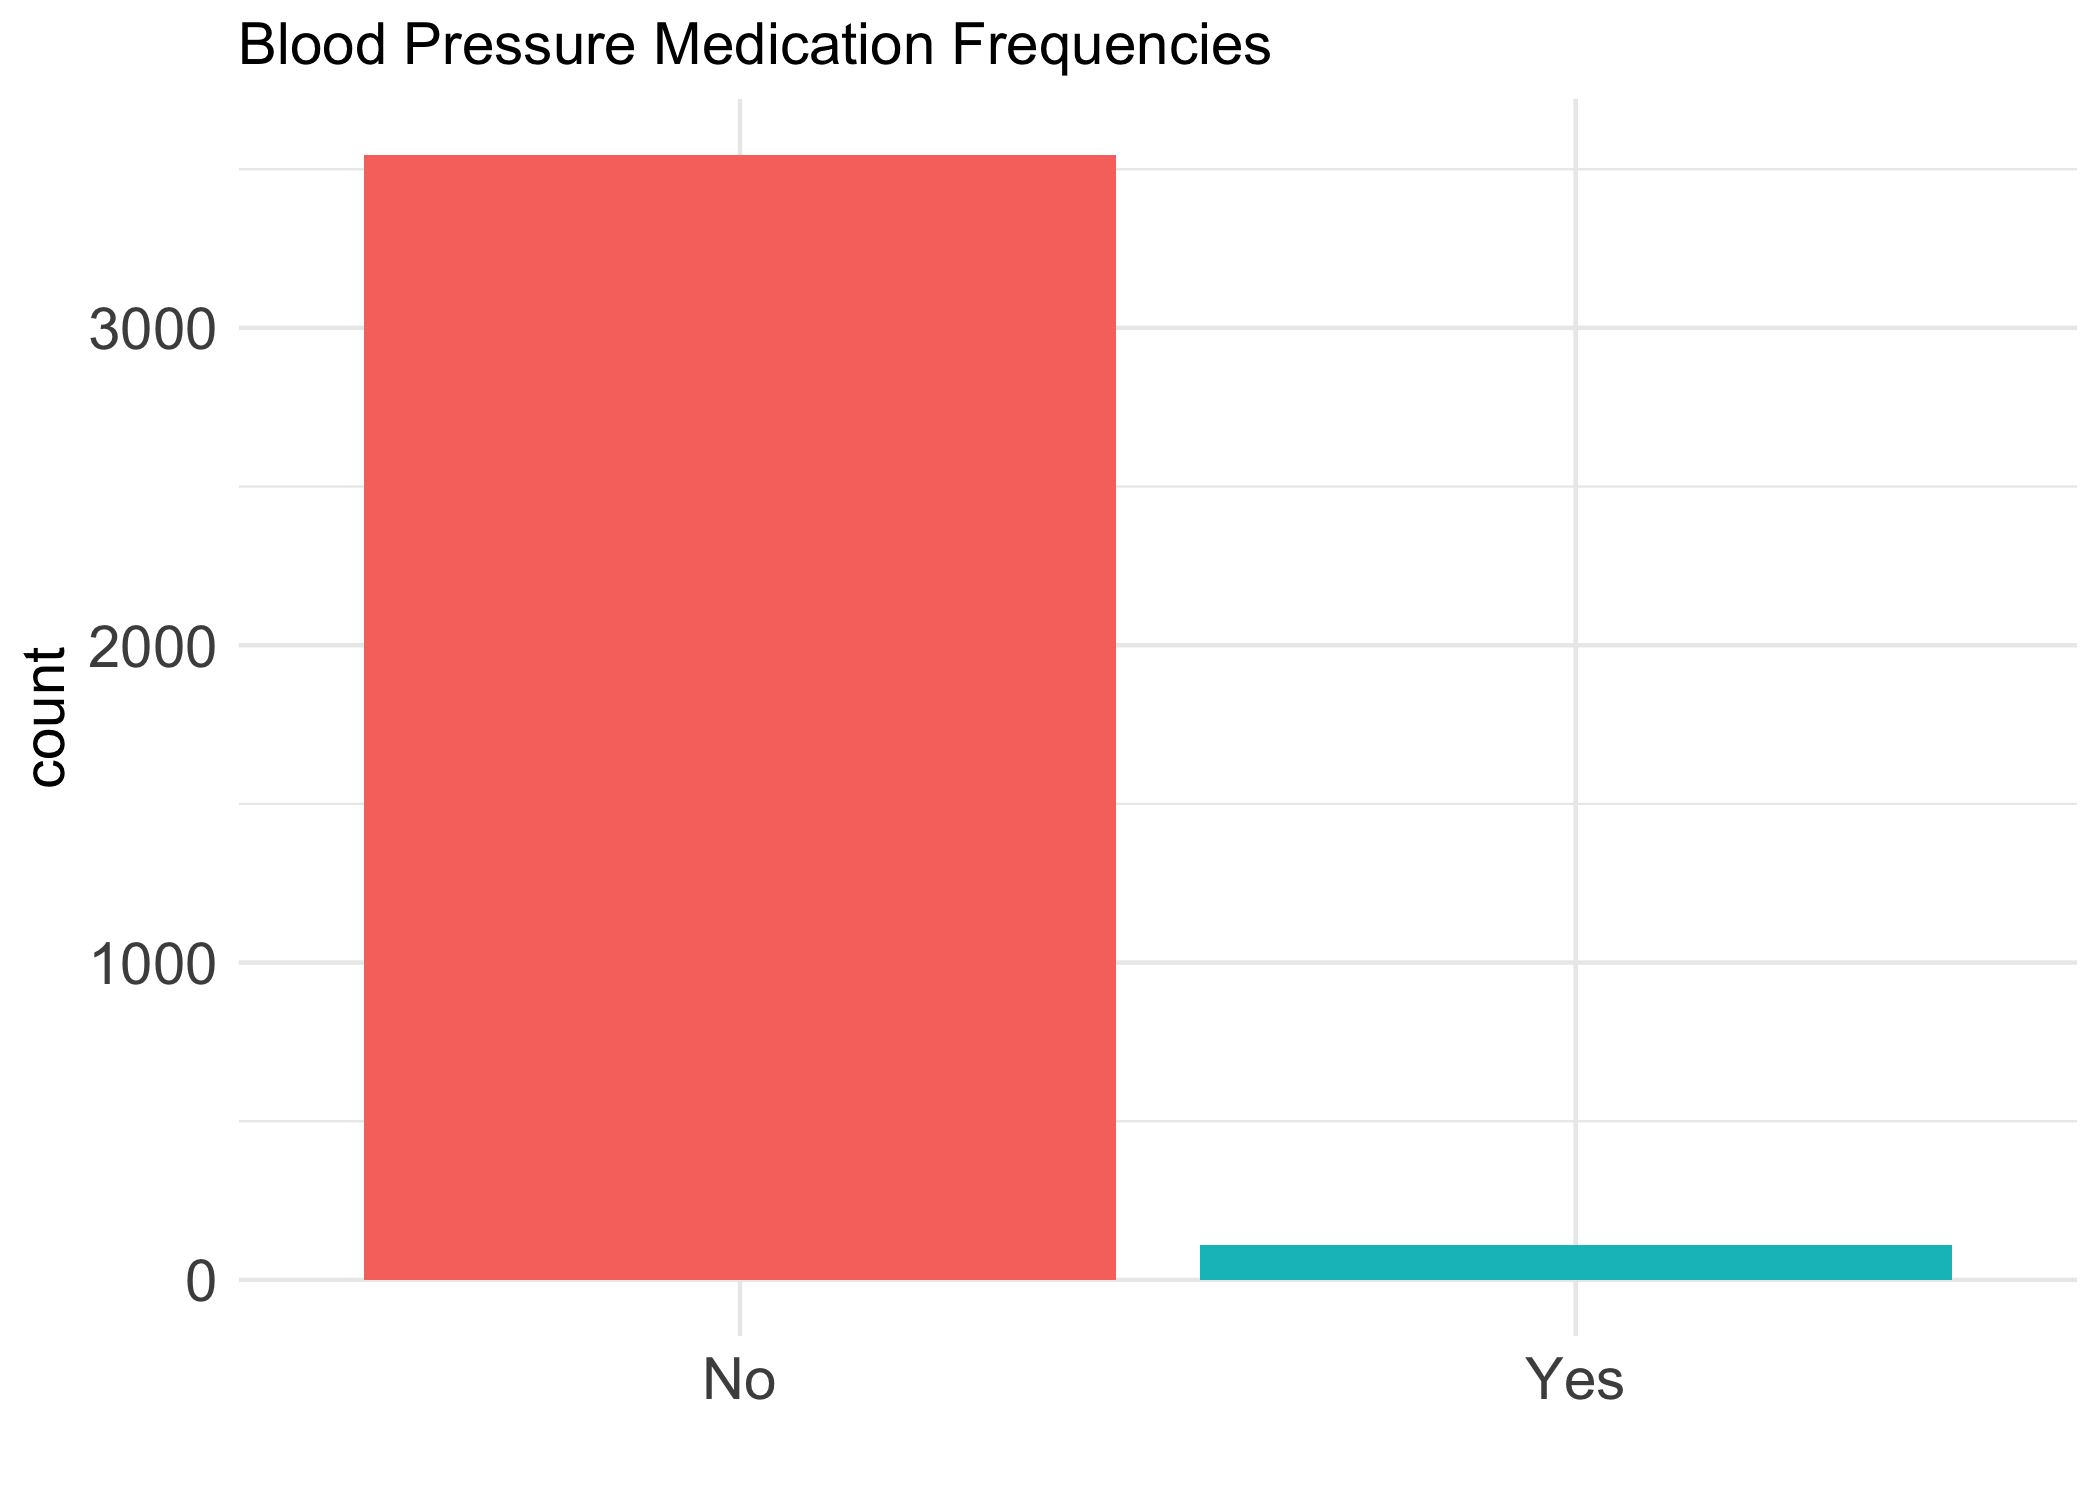
\includegraphics[height=45mm, width=65mm]{bar_bp_meds.png}}\hspace{2em}%
\subcaptionbox*{}{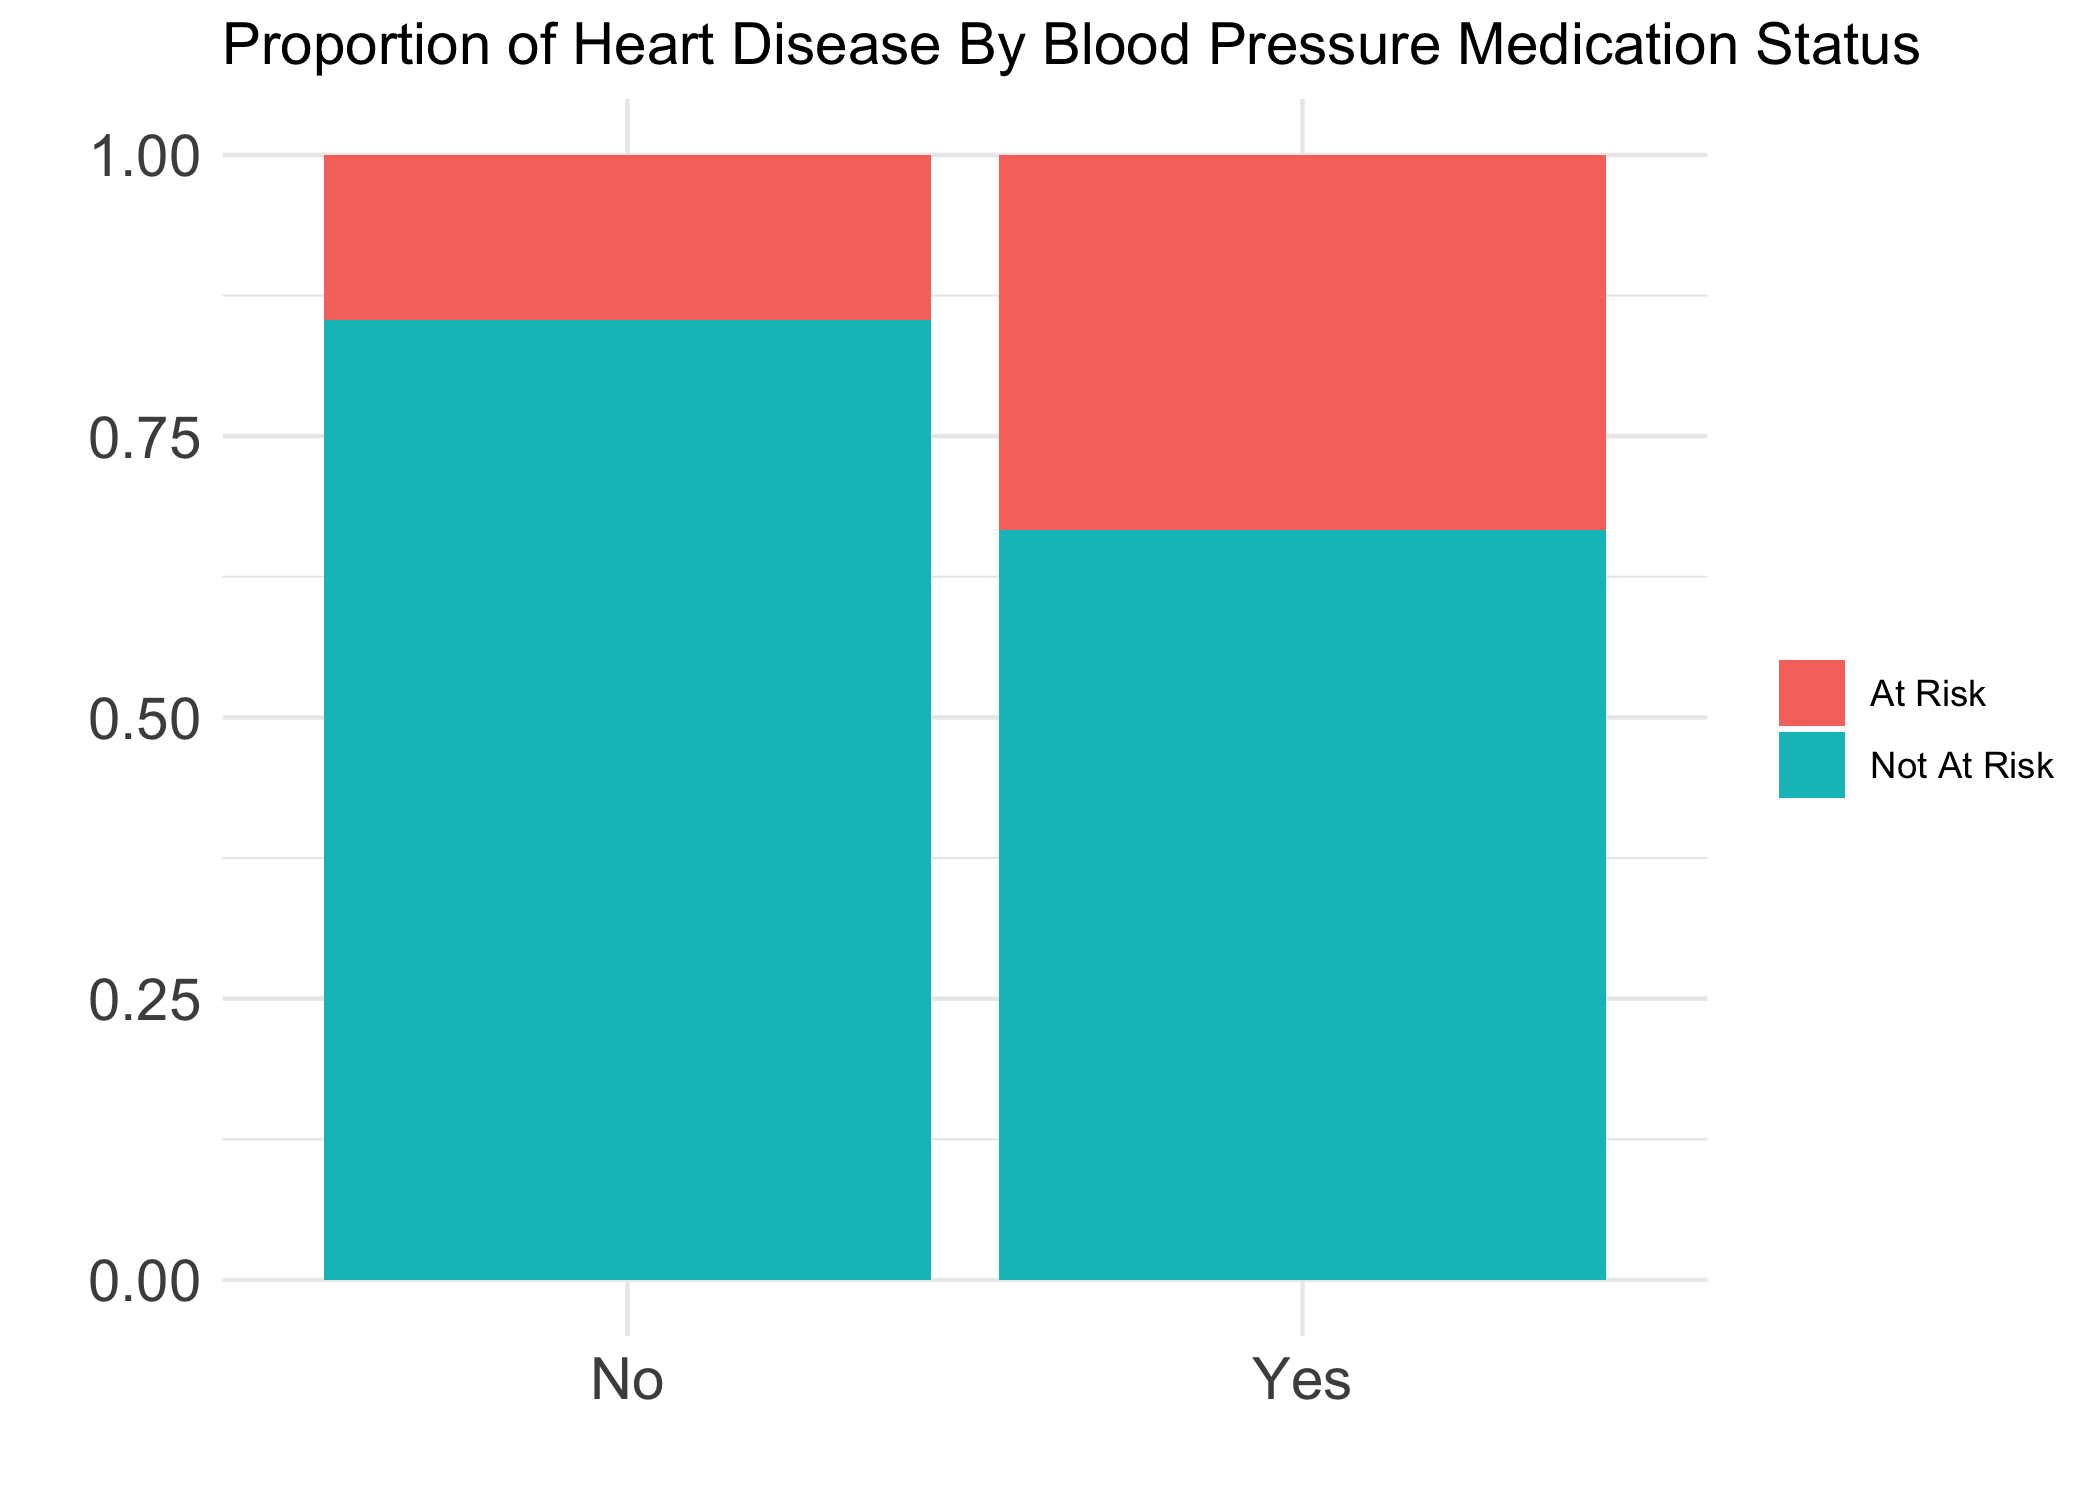
\includegraphics[height=45mm, width=65mm]{two_way_bp_meds.png}}%
\hspace*{\fill}
\end{figure}


\subsubsection*{Prevalent Stroke}

Similarly to blood pressure medication, the majority of patients do not have a history of stroke. As expected, the proportion of patients at risk for 10-year coronary heart disease is greater among patients who have had a stroke. In fact, if a patient in our study has had a stroke, they are twice as likely to be at risk for 10-year coronary heart disease compared to a patient who has not had a stroke.

\begin{figure}[hbt!]
\hspace*{\fill}
\centering
\subcaptionbox*{}{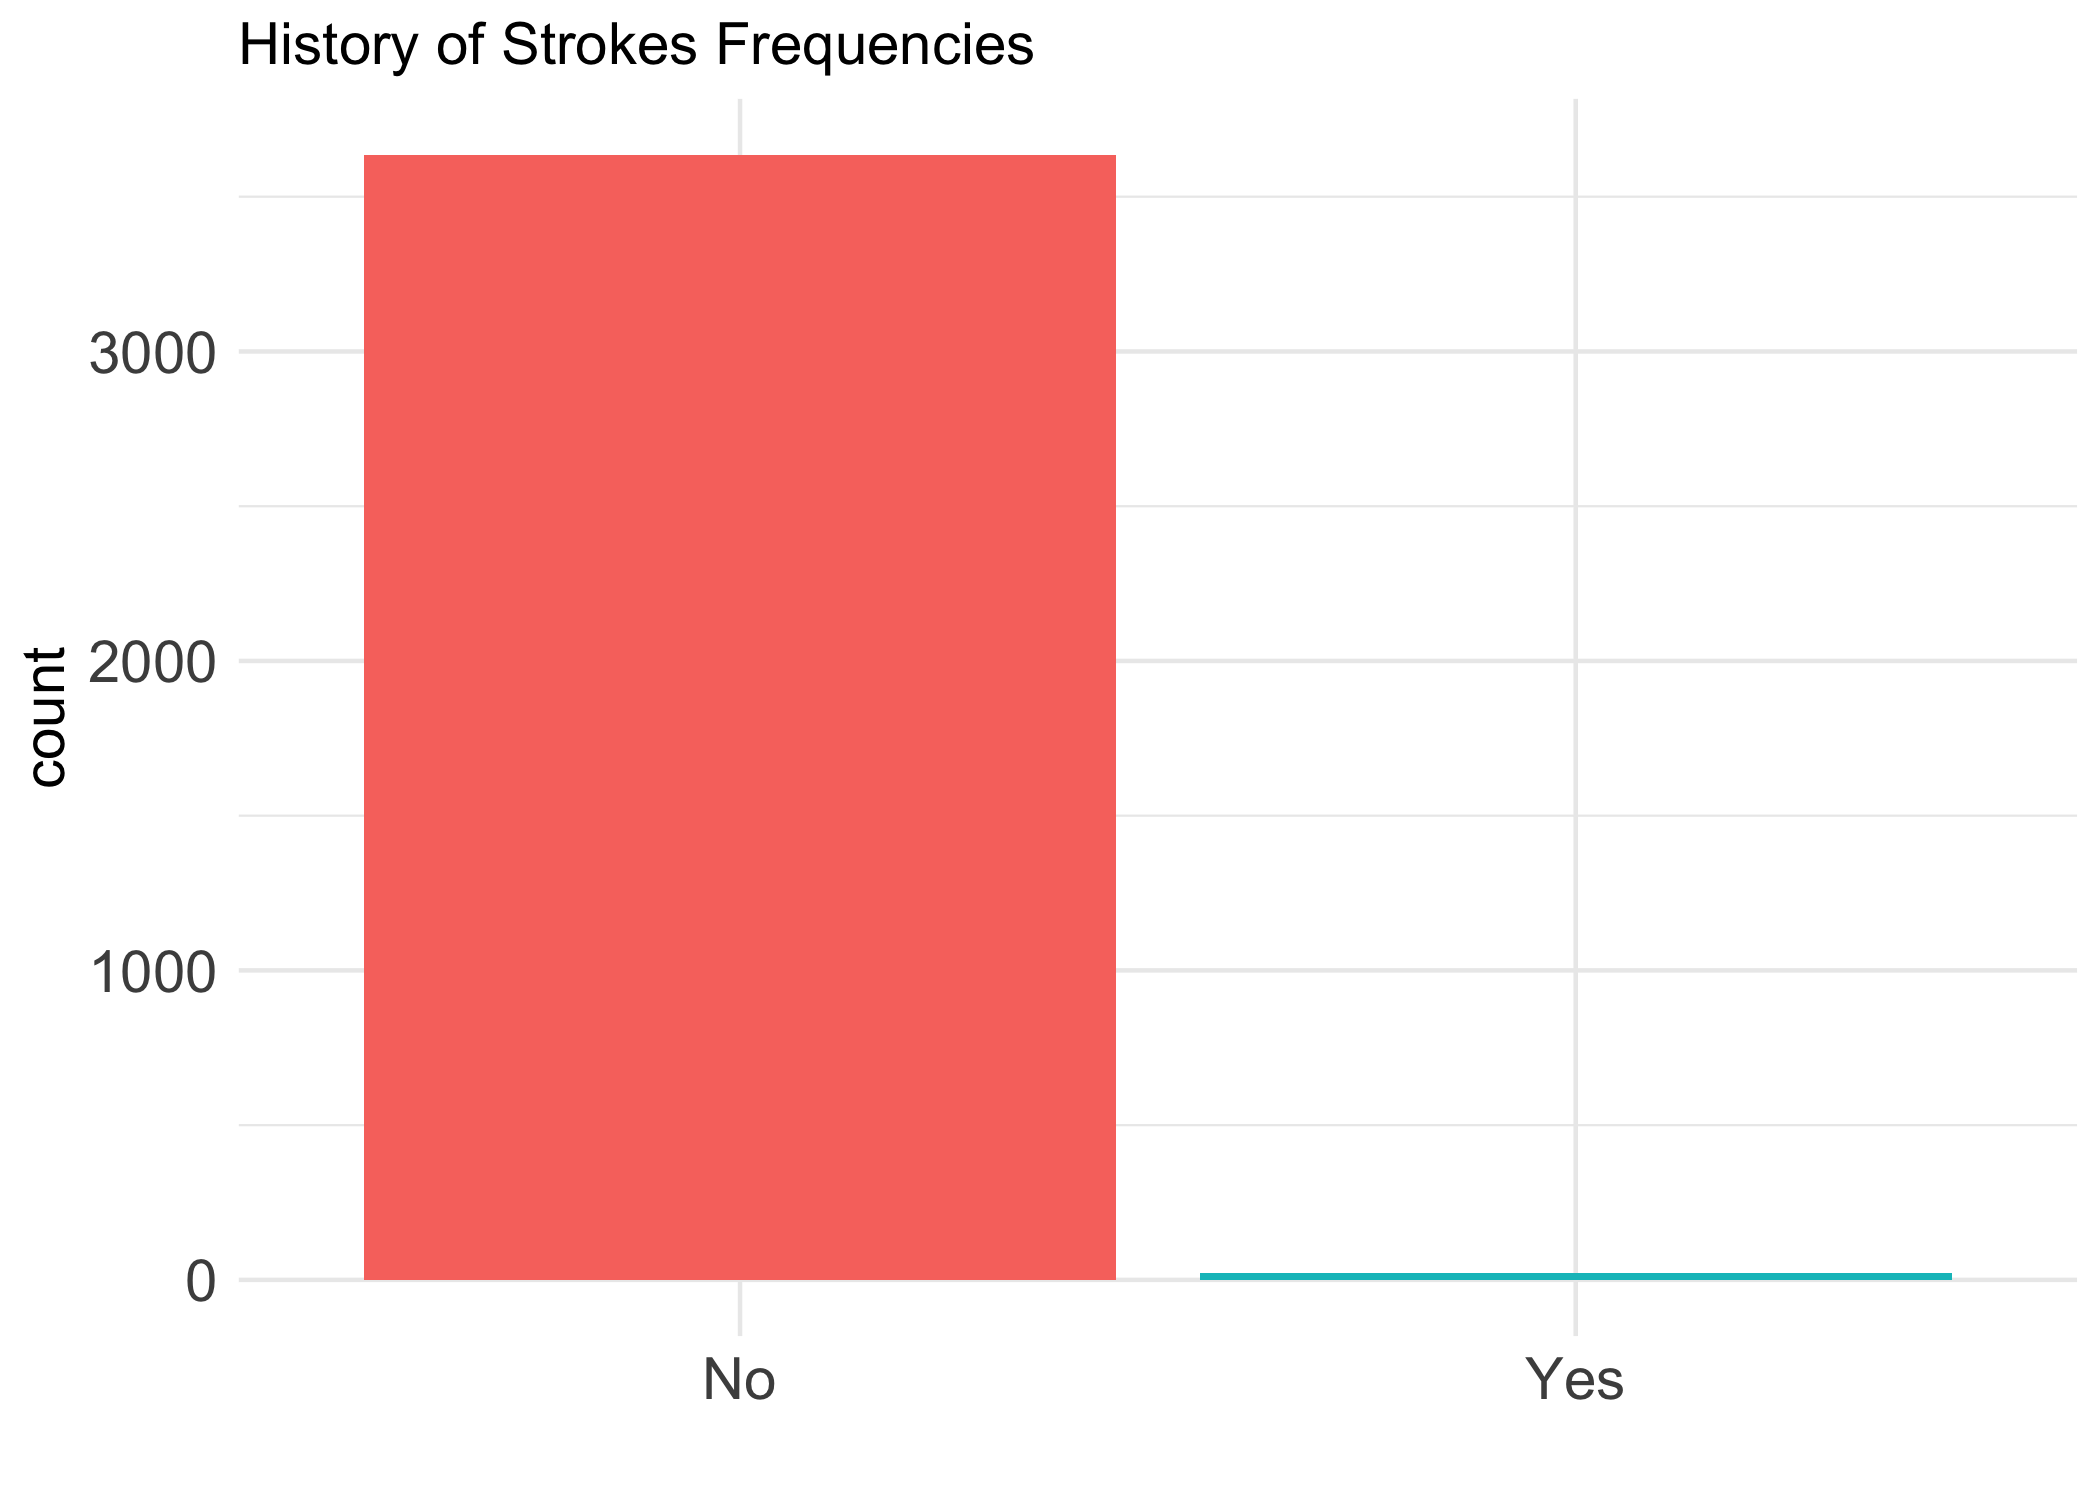
\includegraphics[height=45mm, width=65mm]{bar_strokes.png}}\hspace{2em}%
\subcaptionbox*{}{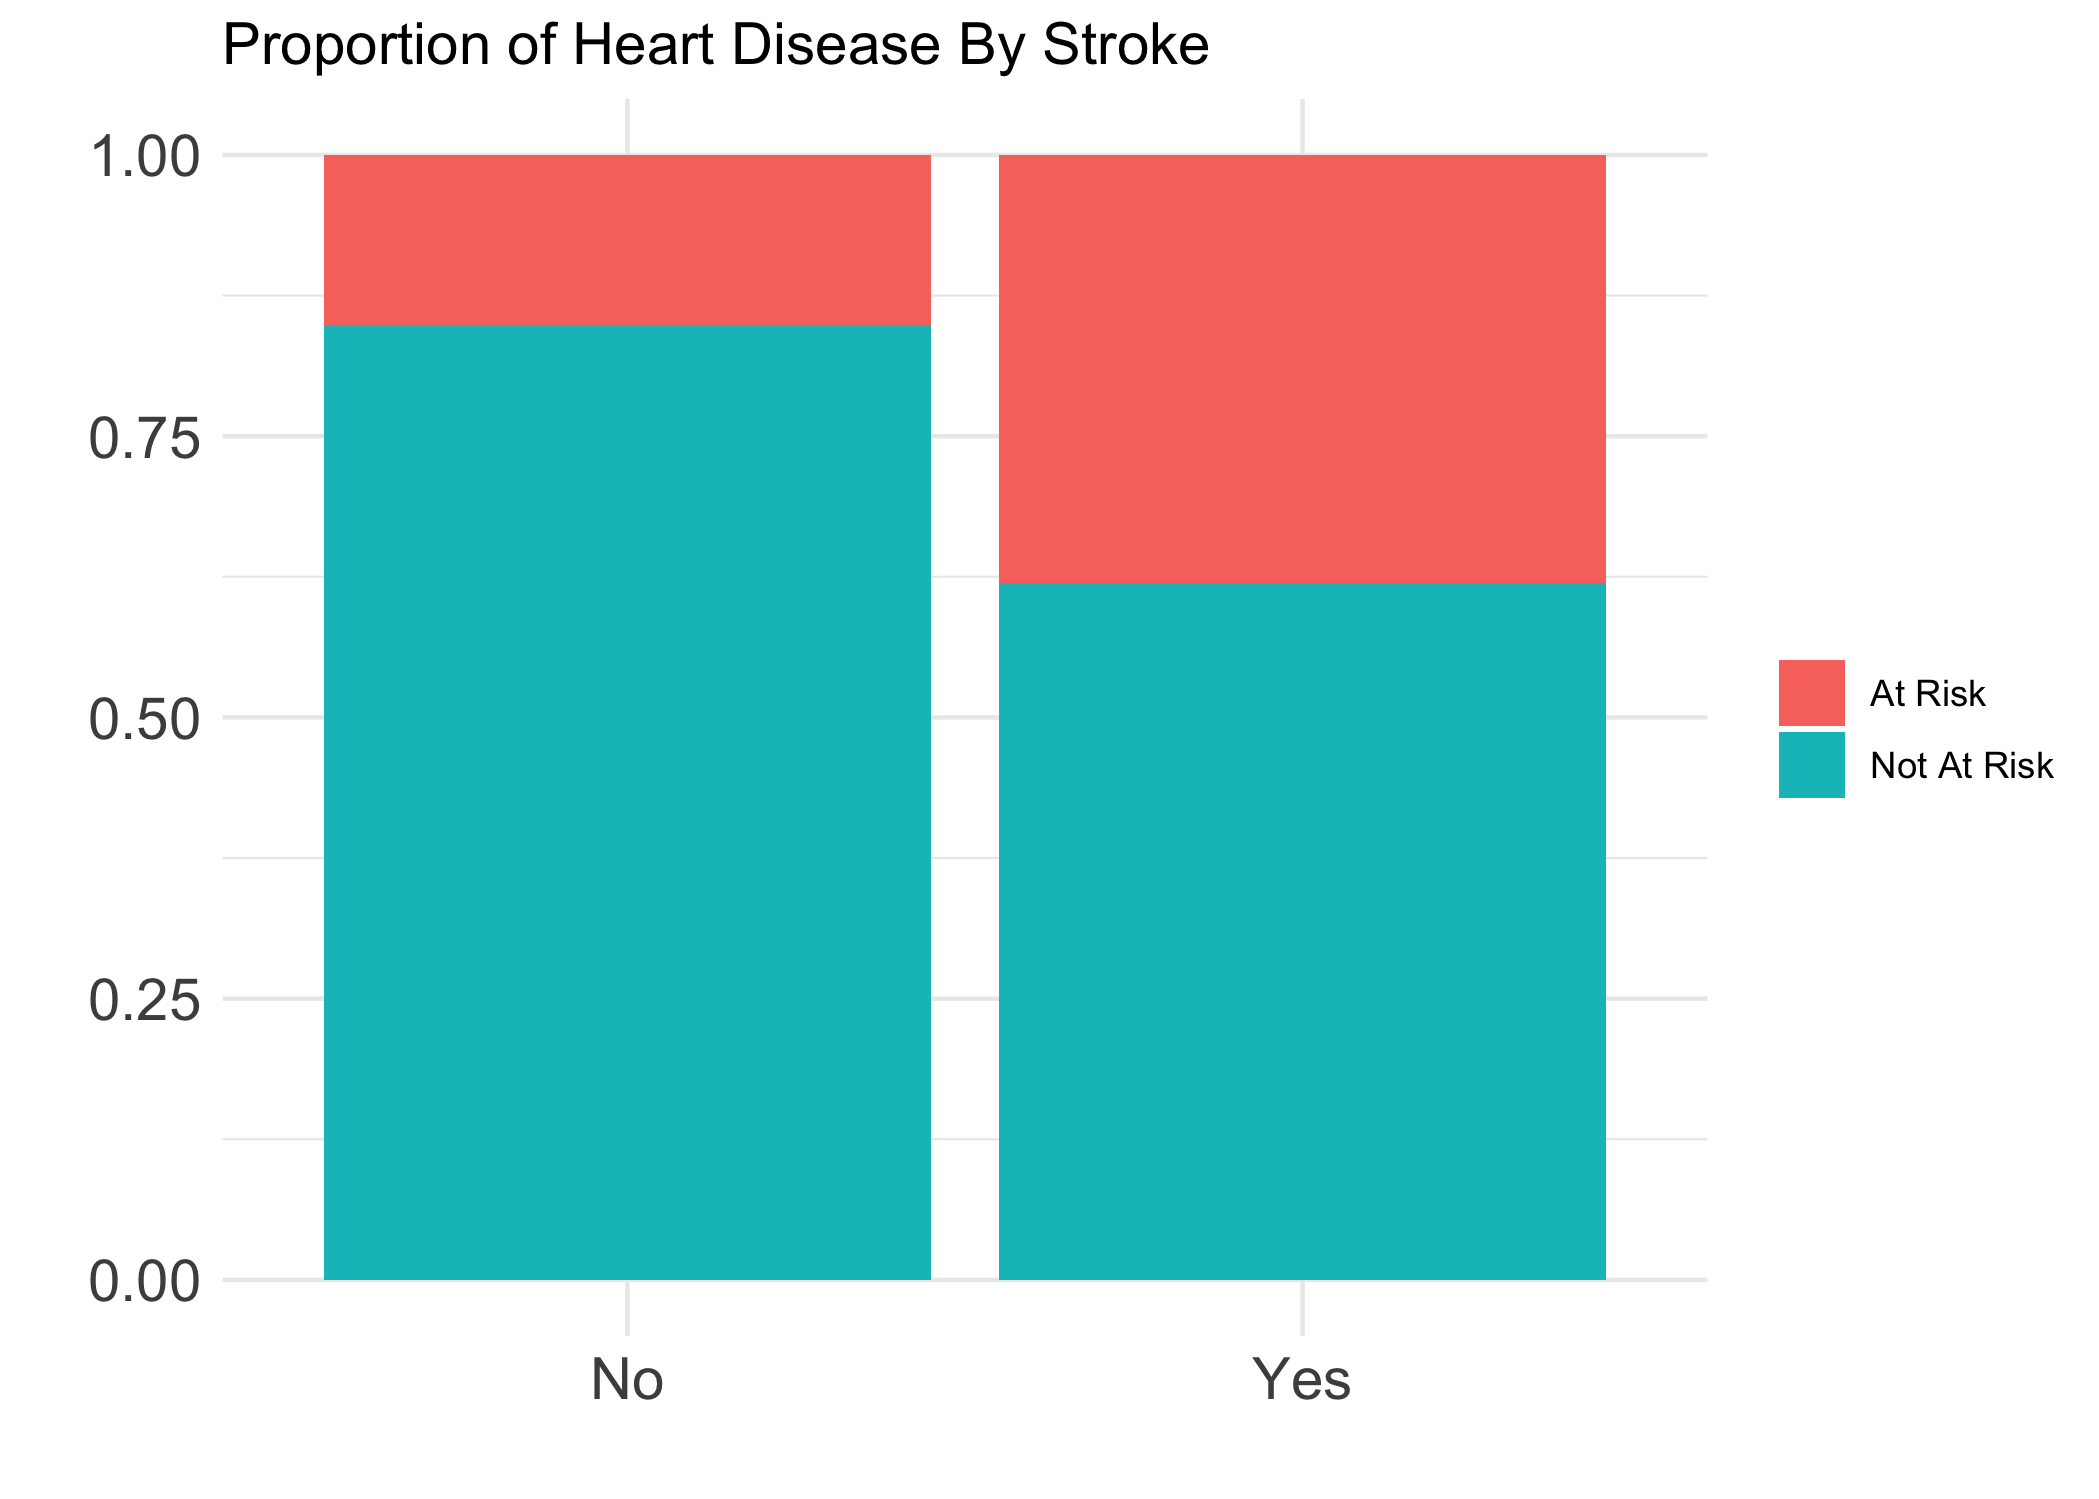
\includegraphics[height=45mm, width=65mm]{two_way_stroke.png}}%
\hspace*{\fill}
\end{figure}


\subsubsection*{Prevalent Hypertension}

Nearly one-third of patients in the study do not have hypertension. Similarly to prevalent strokes, if a patient in our study has hypertension, they are twice as likely to be at risk for 10-year coronary heart disease. 

\begin{figure}[hbt!]
\hspace*{\fill}
\centering
\subcaptionbox*{}{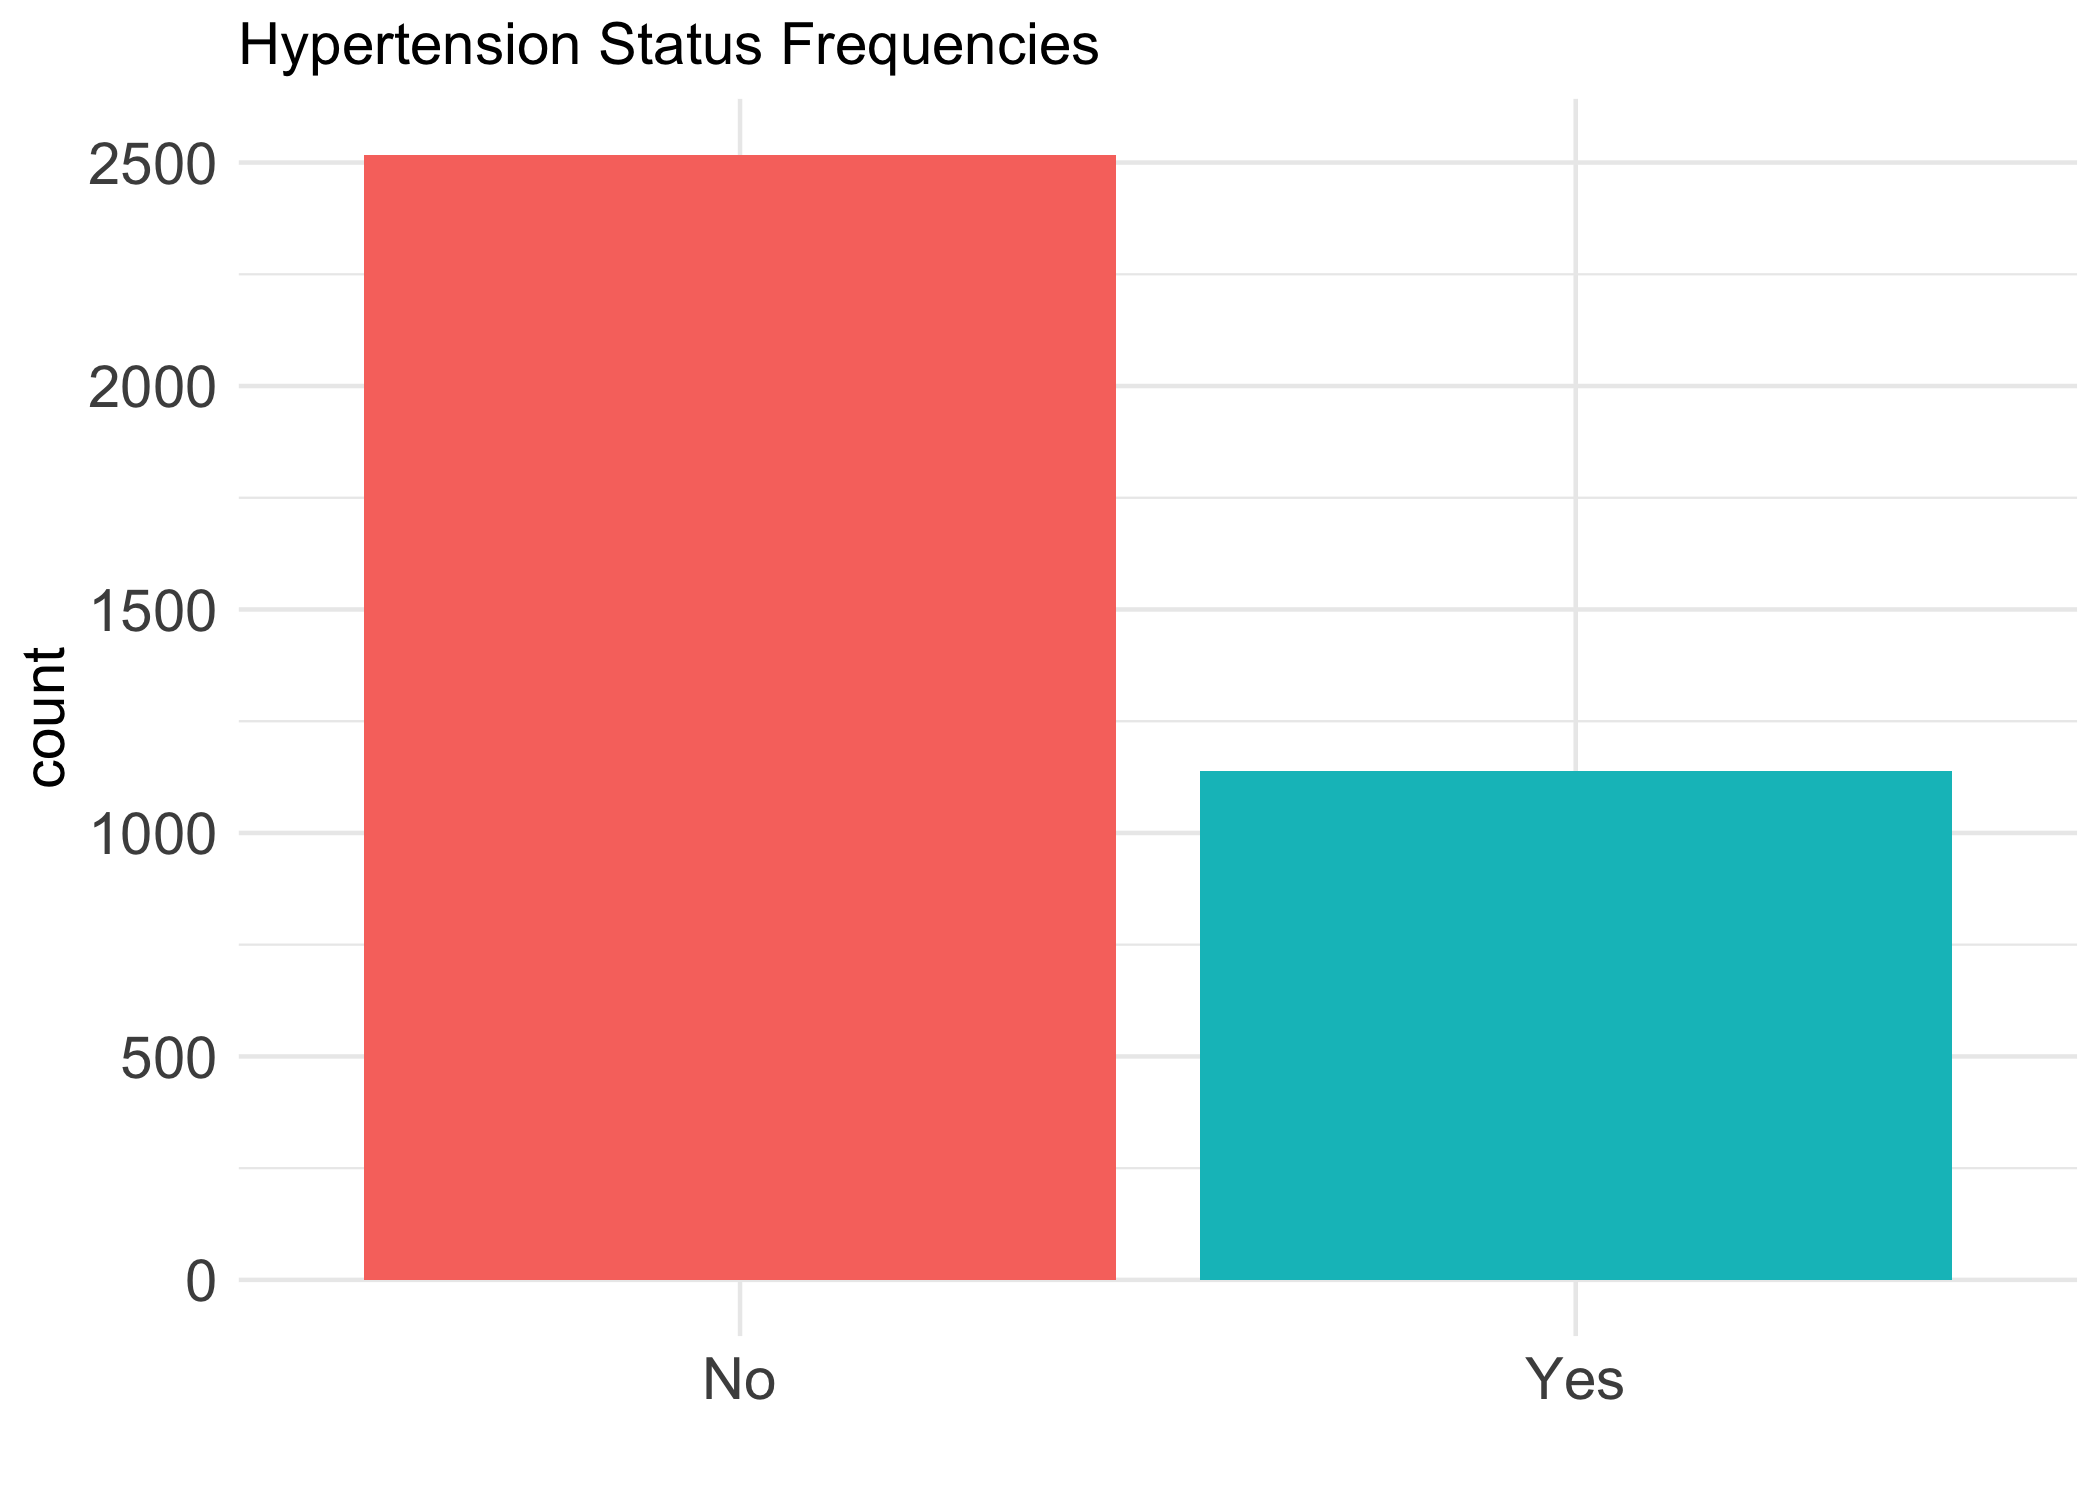
\includegraphics[height=45mm, width=65mm]{bar_hypertension.png}}\hspace{2em}%
\subcaptionbox*{}{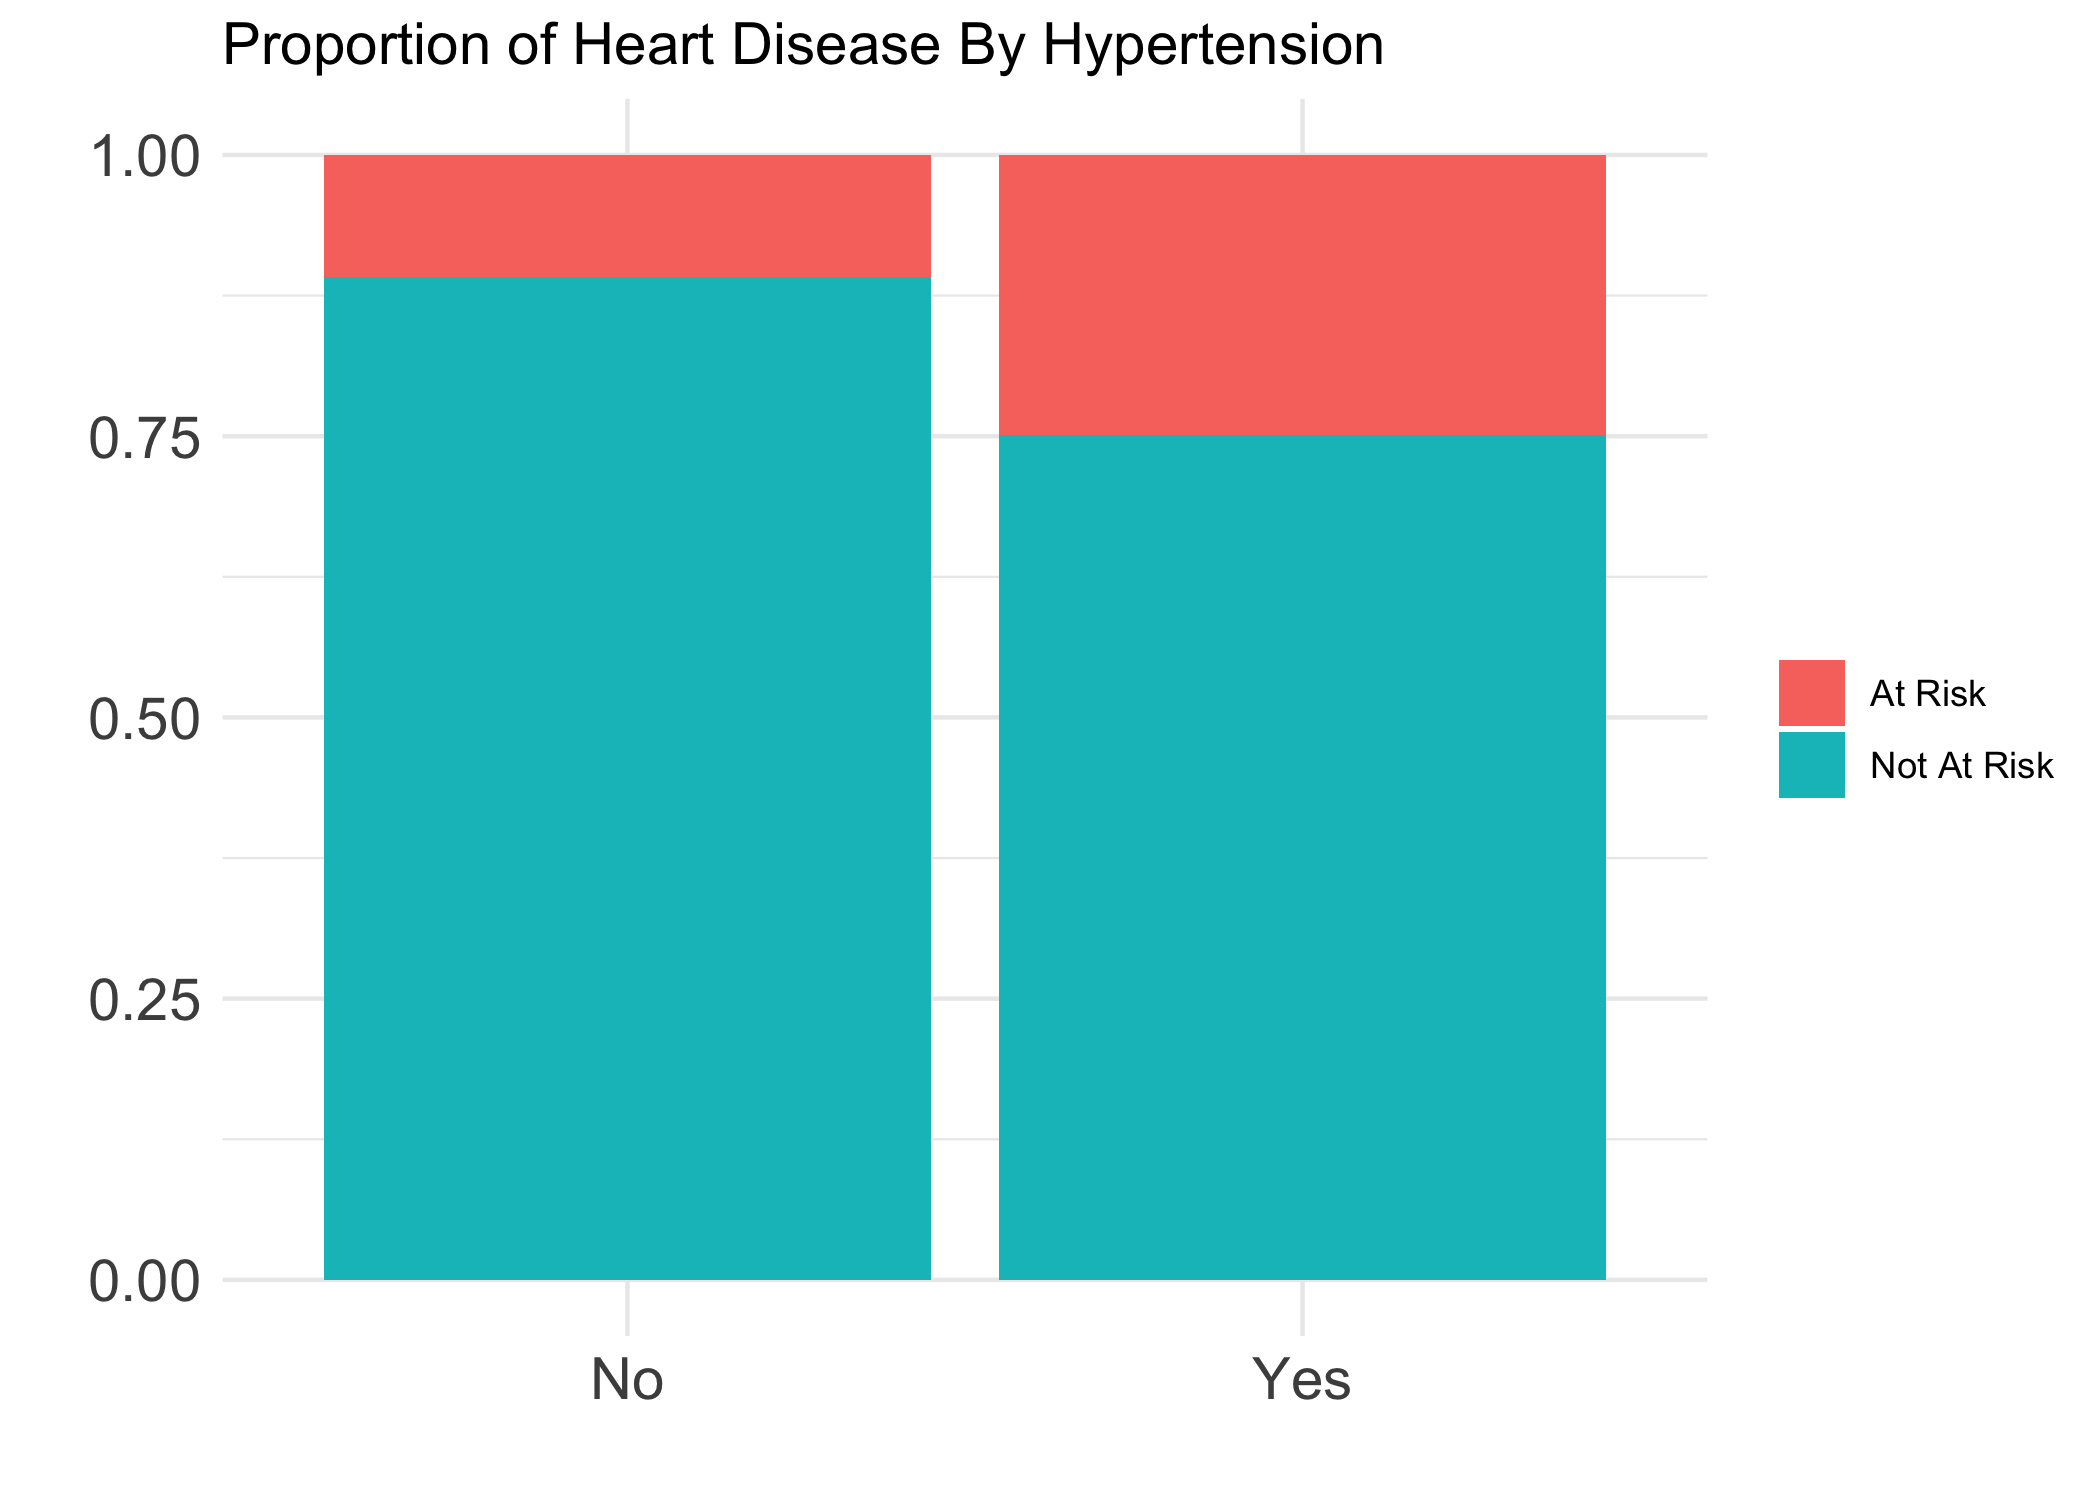
\includegraphics[height=45mm, width=65mm]{two_way_hypertension.png}}%
\hspace*{\fill}
\end{figure}

\subsubsection*{Diabetes}

The majority of patients do not have diabetes, and yet, approximately 15\% of these patients are at risk for 10-year coronary heart disease. On the other hand, over 30\% of patients with diabetes are at risk for 10-year coronary heart disease.

\begin{figure}[hbt!]
\hspace*{\fill}
\centering
\subcaptionbox*{}{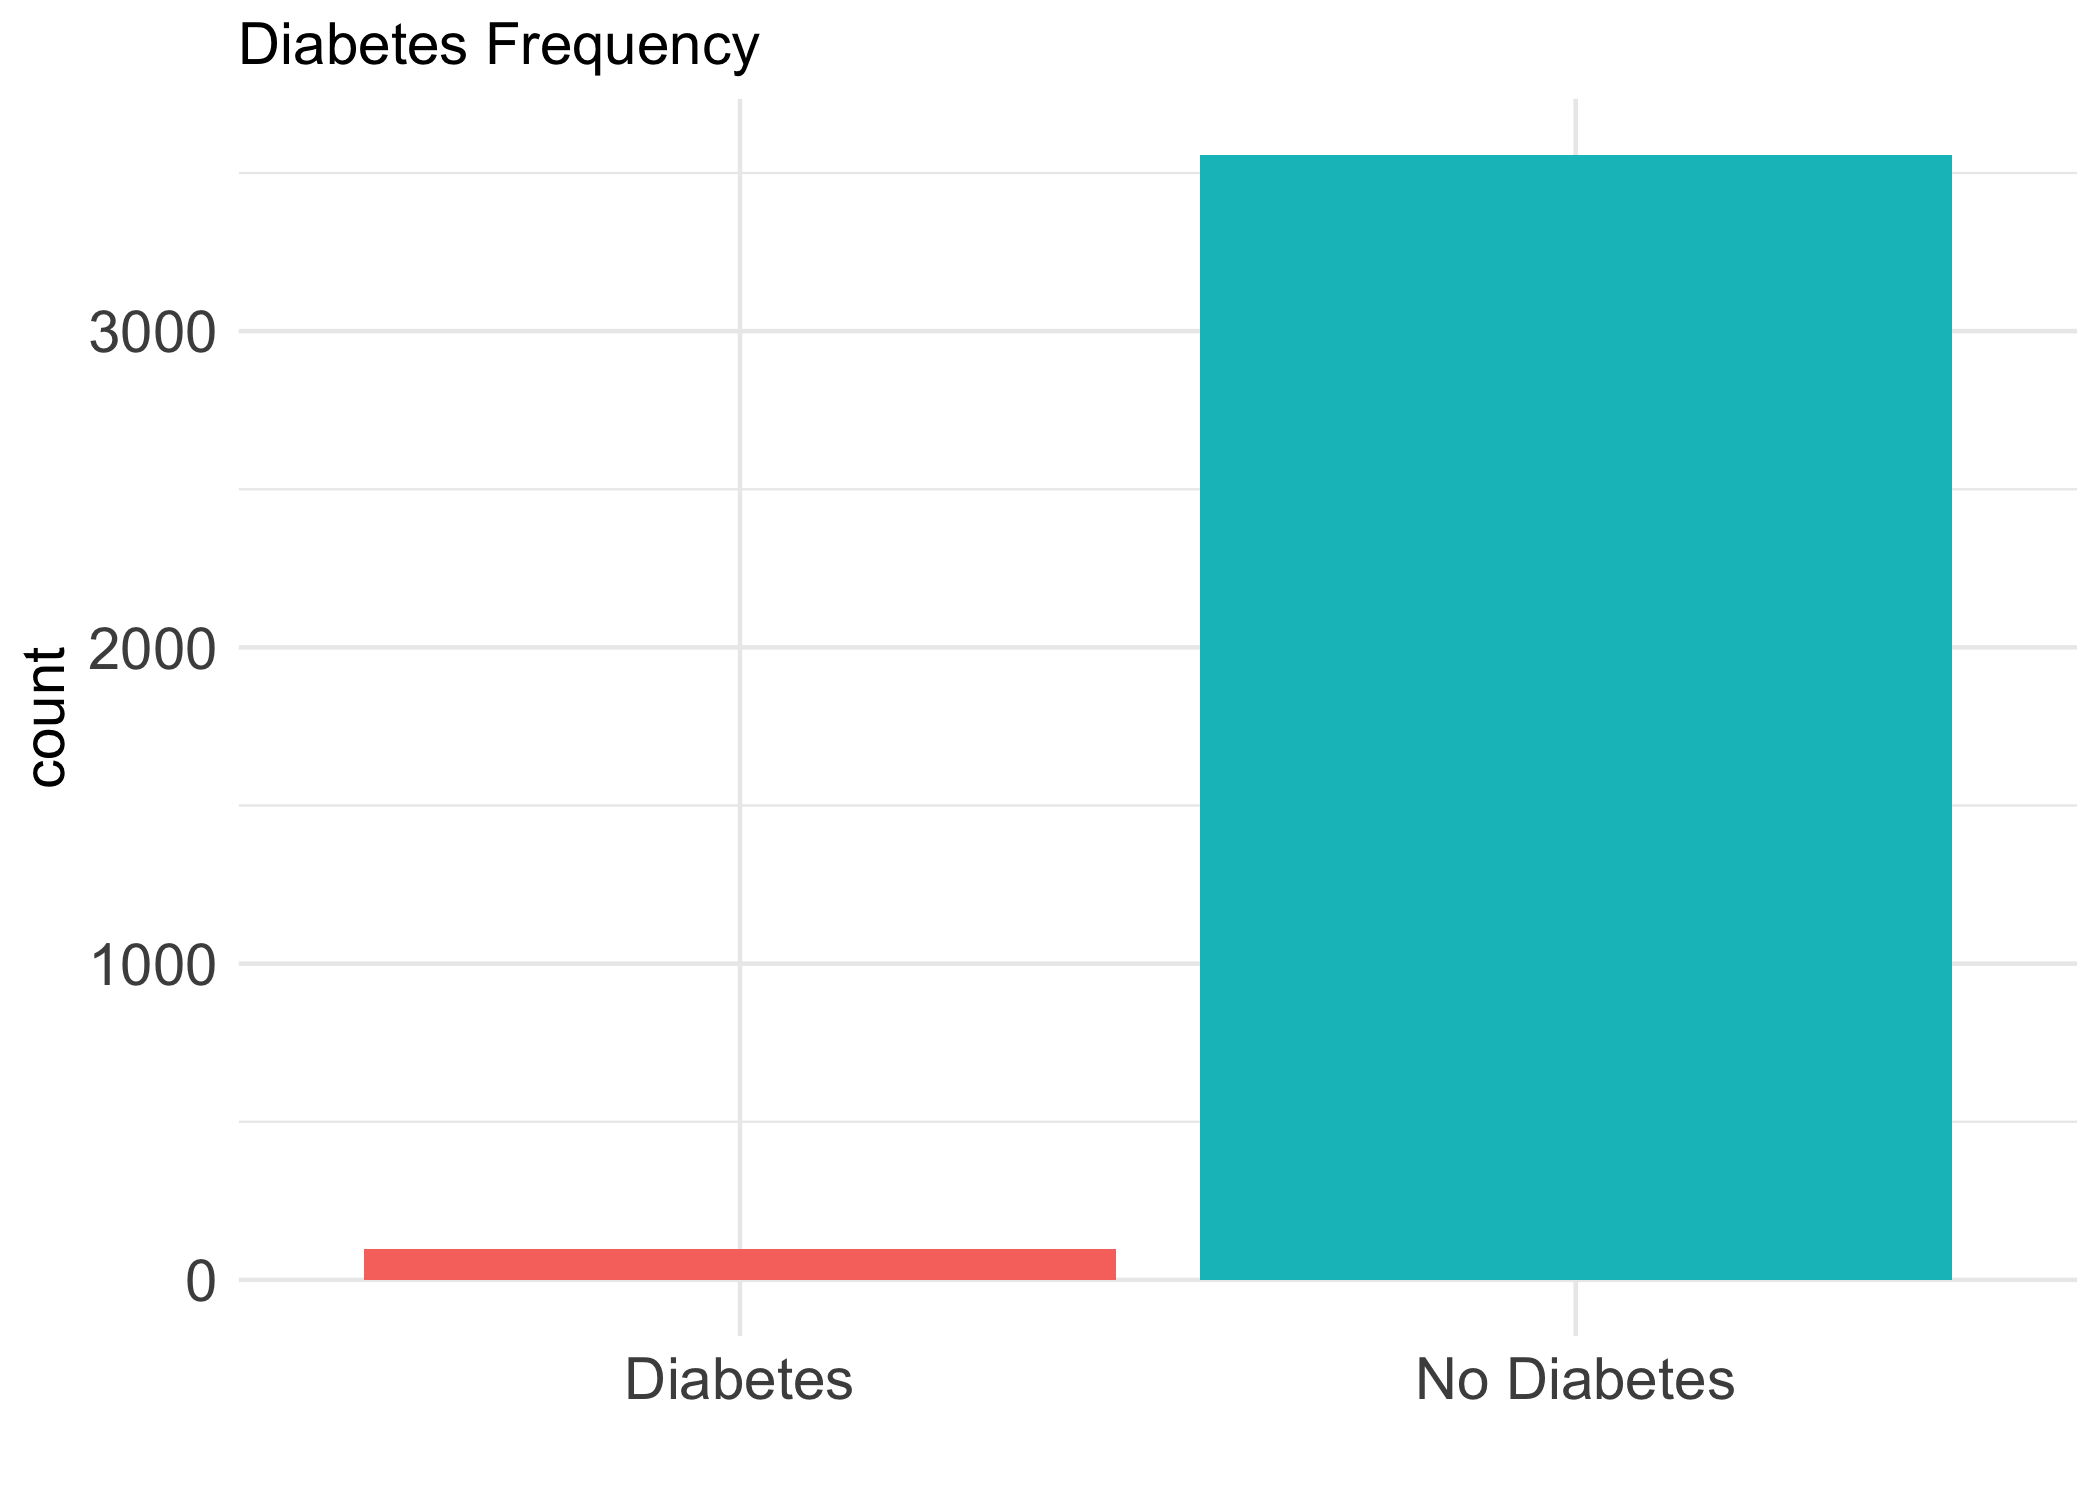
\includegraphics[height=45mm, width=65mm]{bar_diabetes.png}}\hspace{2em}%
\subcaptionbox*{}{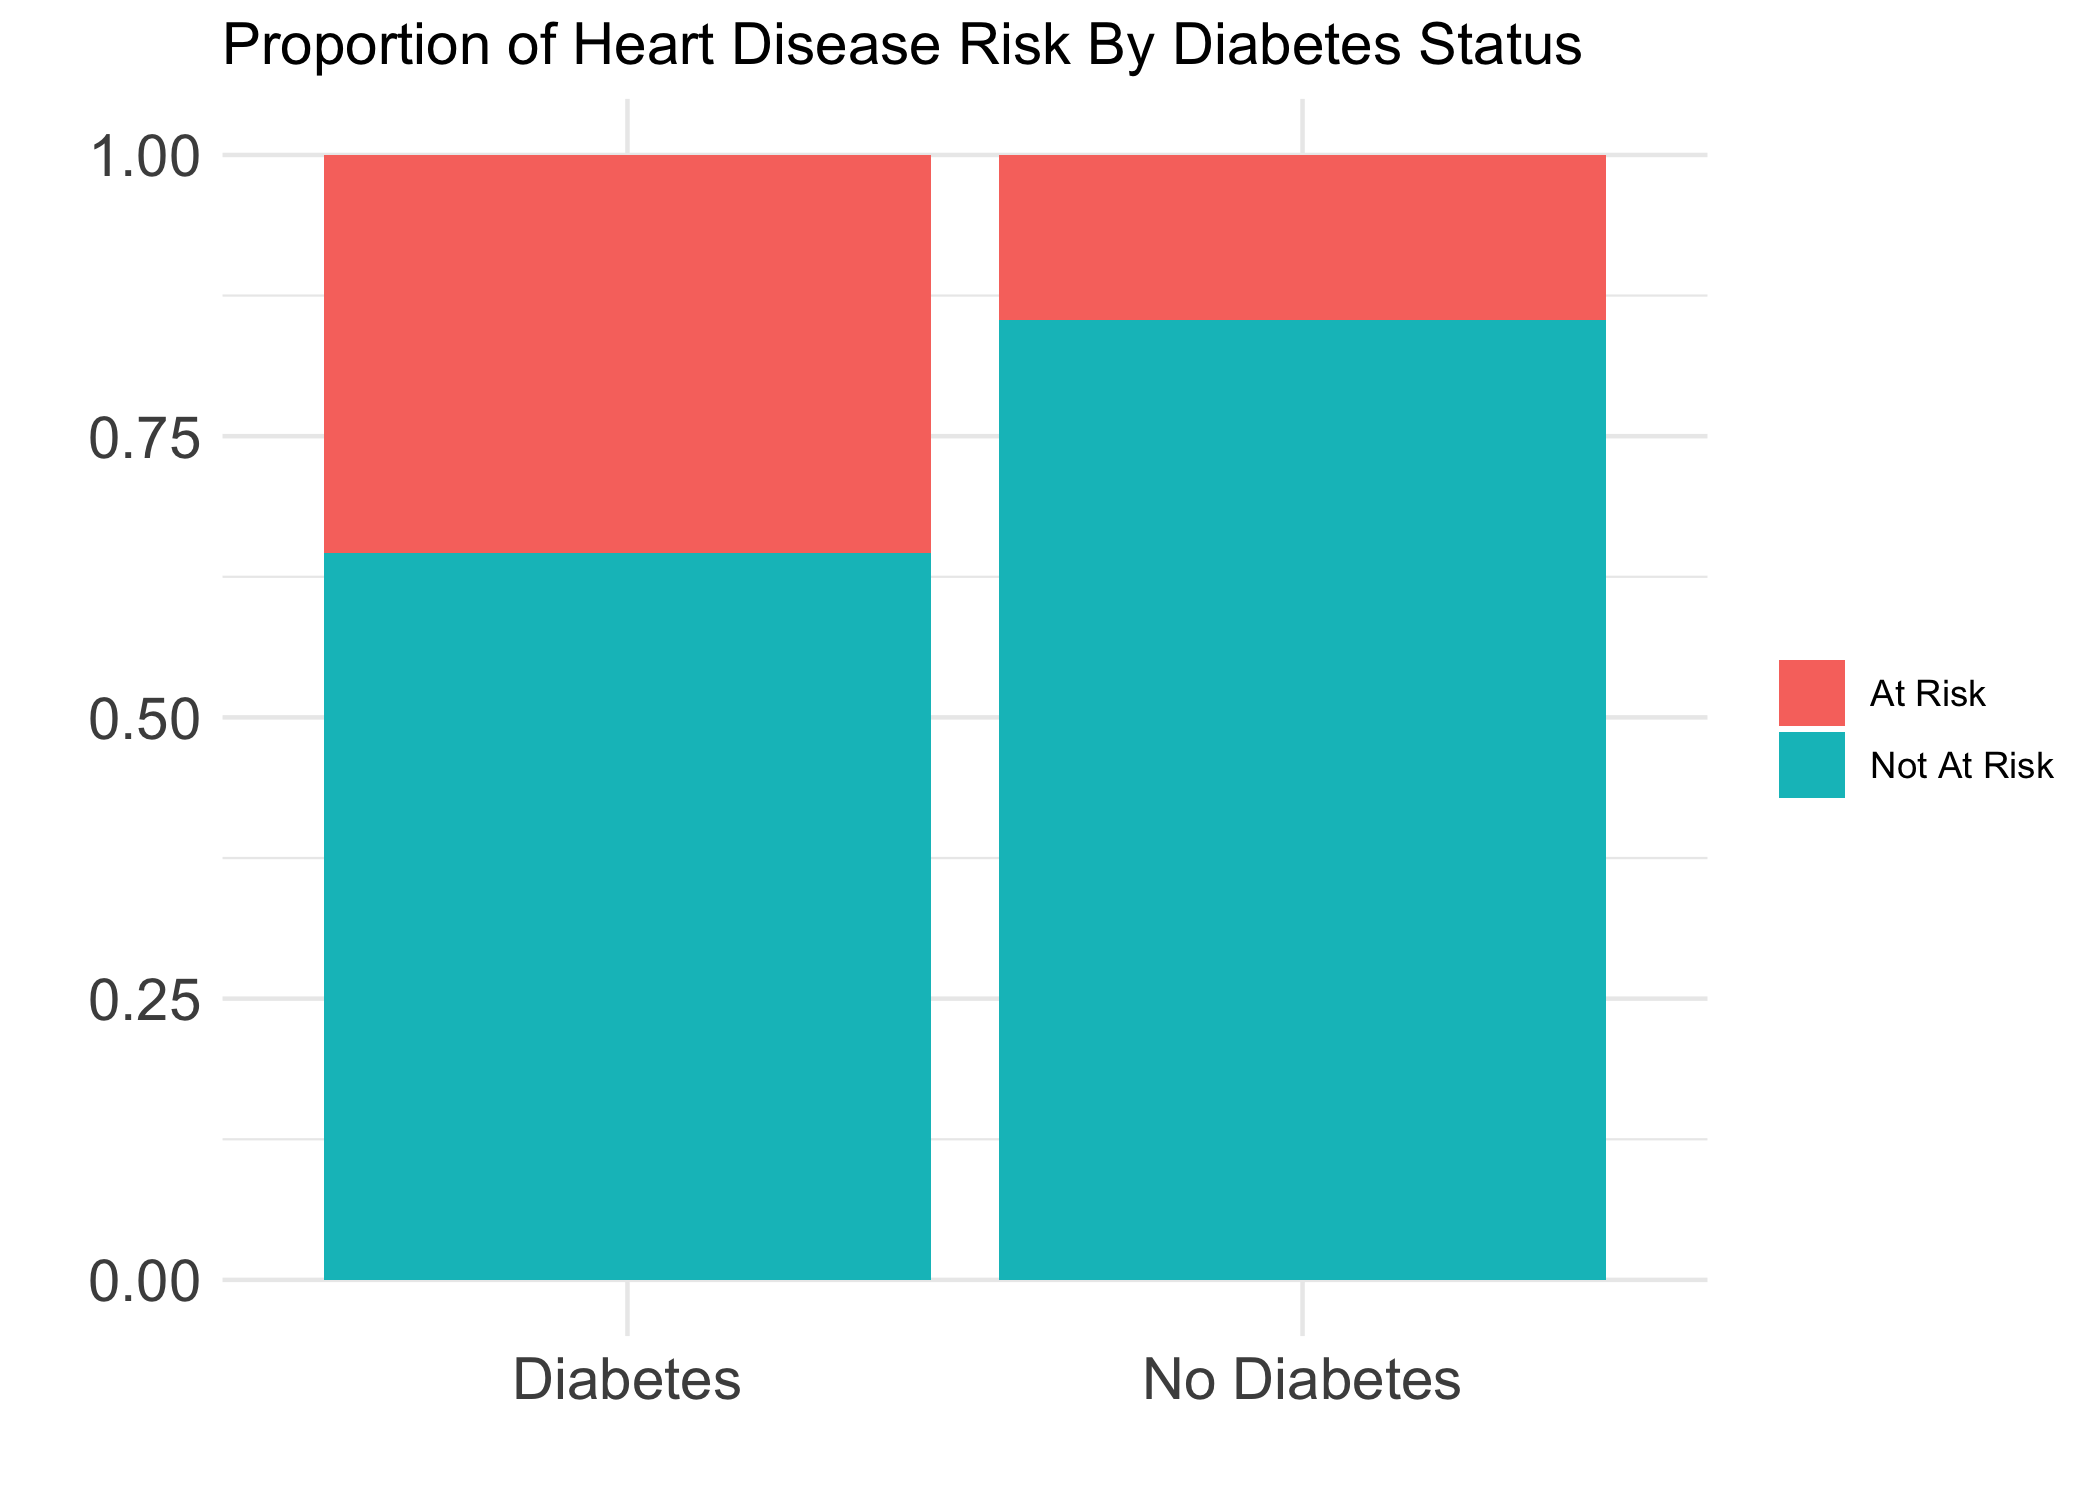
\includegraphics[height=45mm, width=65mm]{two_way_diabetes.png}}%
\hspace*{\fill}
\end{figure}


\subsubsection*{Total Cholesterol}

The distribution of total cholesterol values appears approximately normal. According to the boxplots below, the distribution of total cholesterol values appears to be the same regardless of whether or not patients are at risk for 10-year coronary heart disease.

\begin{figure}[hbt!]
\hspace*{\fill}
\centering
\subcaptionbox*{}{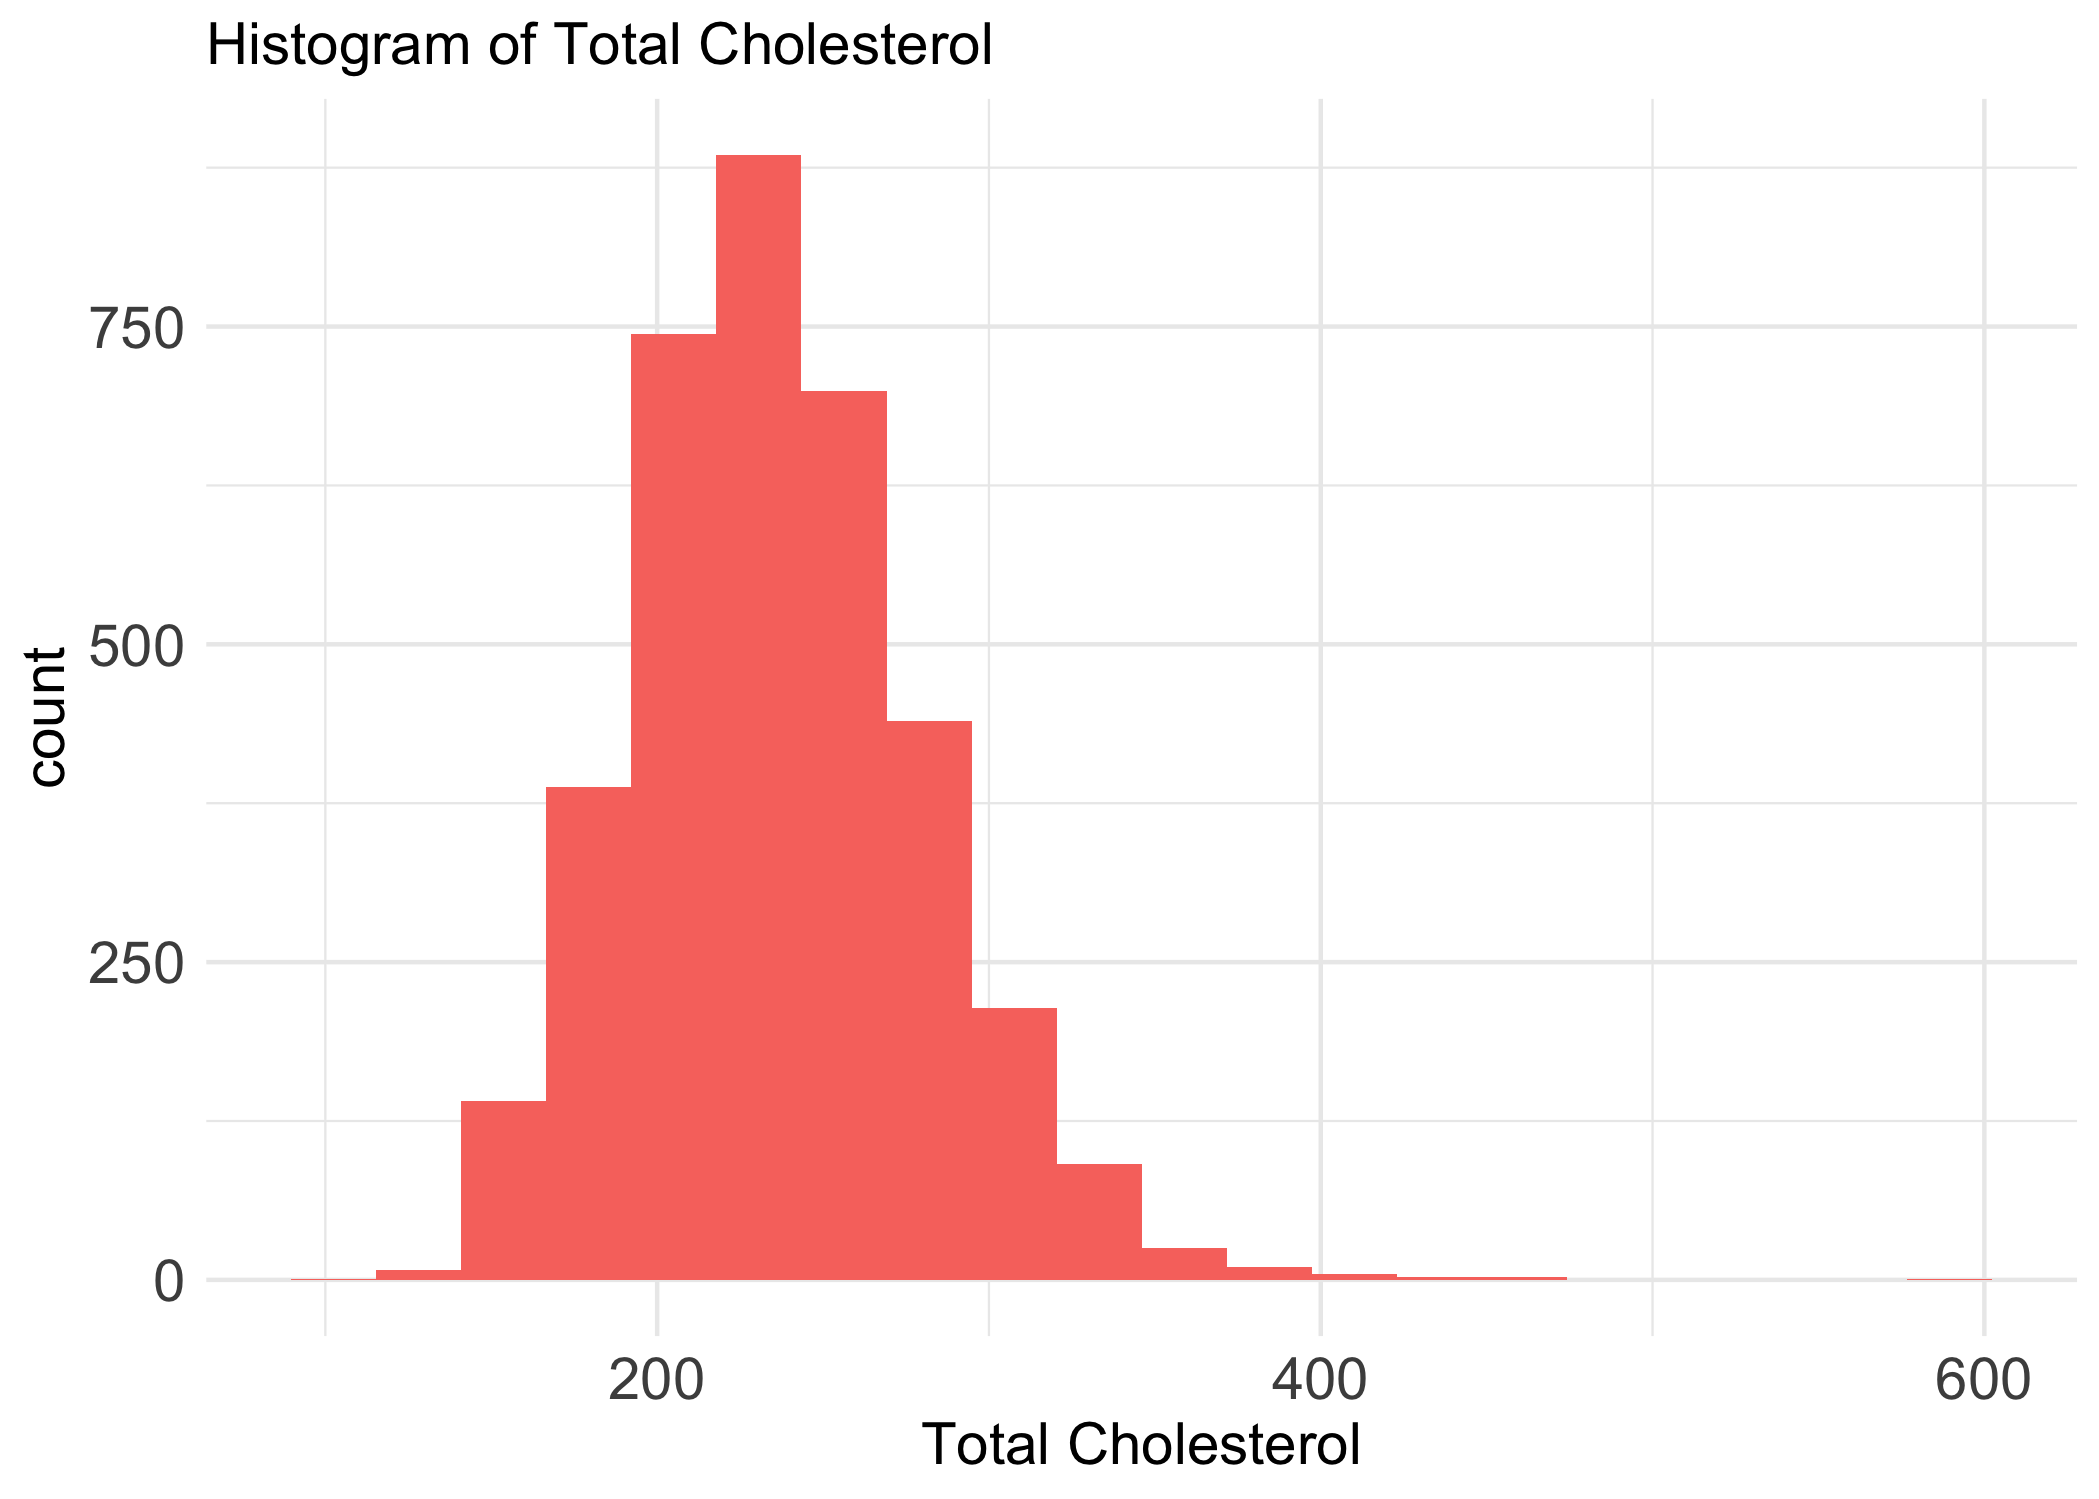
\includegraphics[height=45mm, width=65mm]{hist_cholesterol.png}}\hspace{2em}%
\subcaptionbox*{}{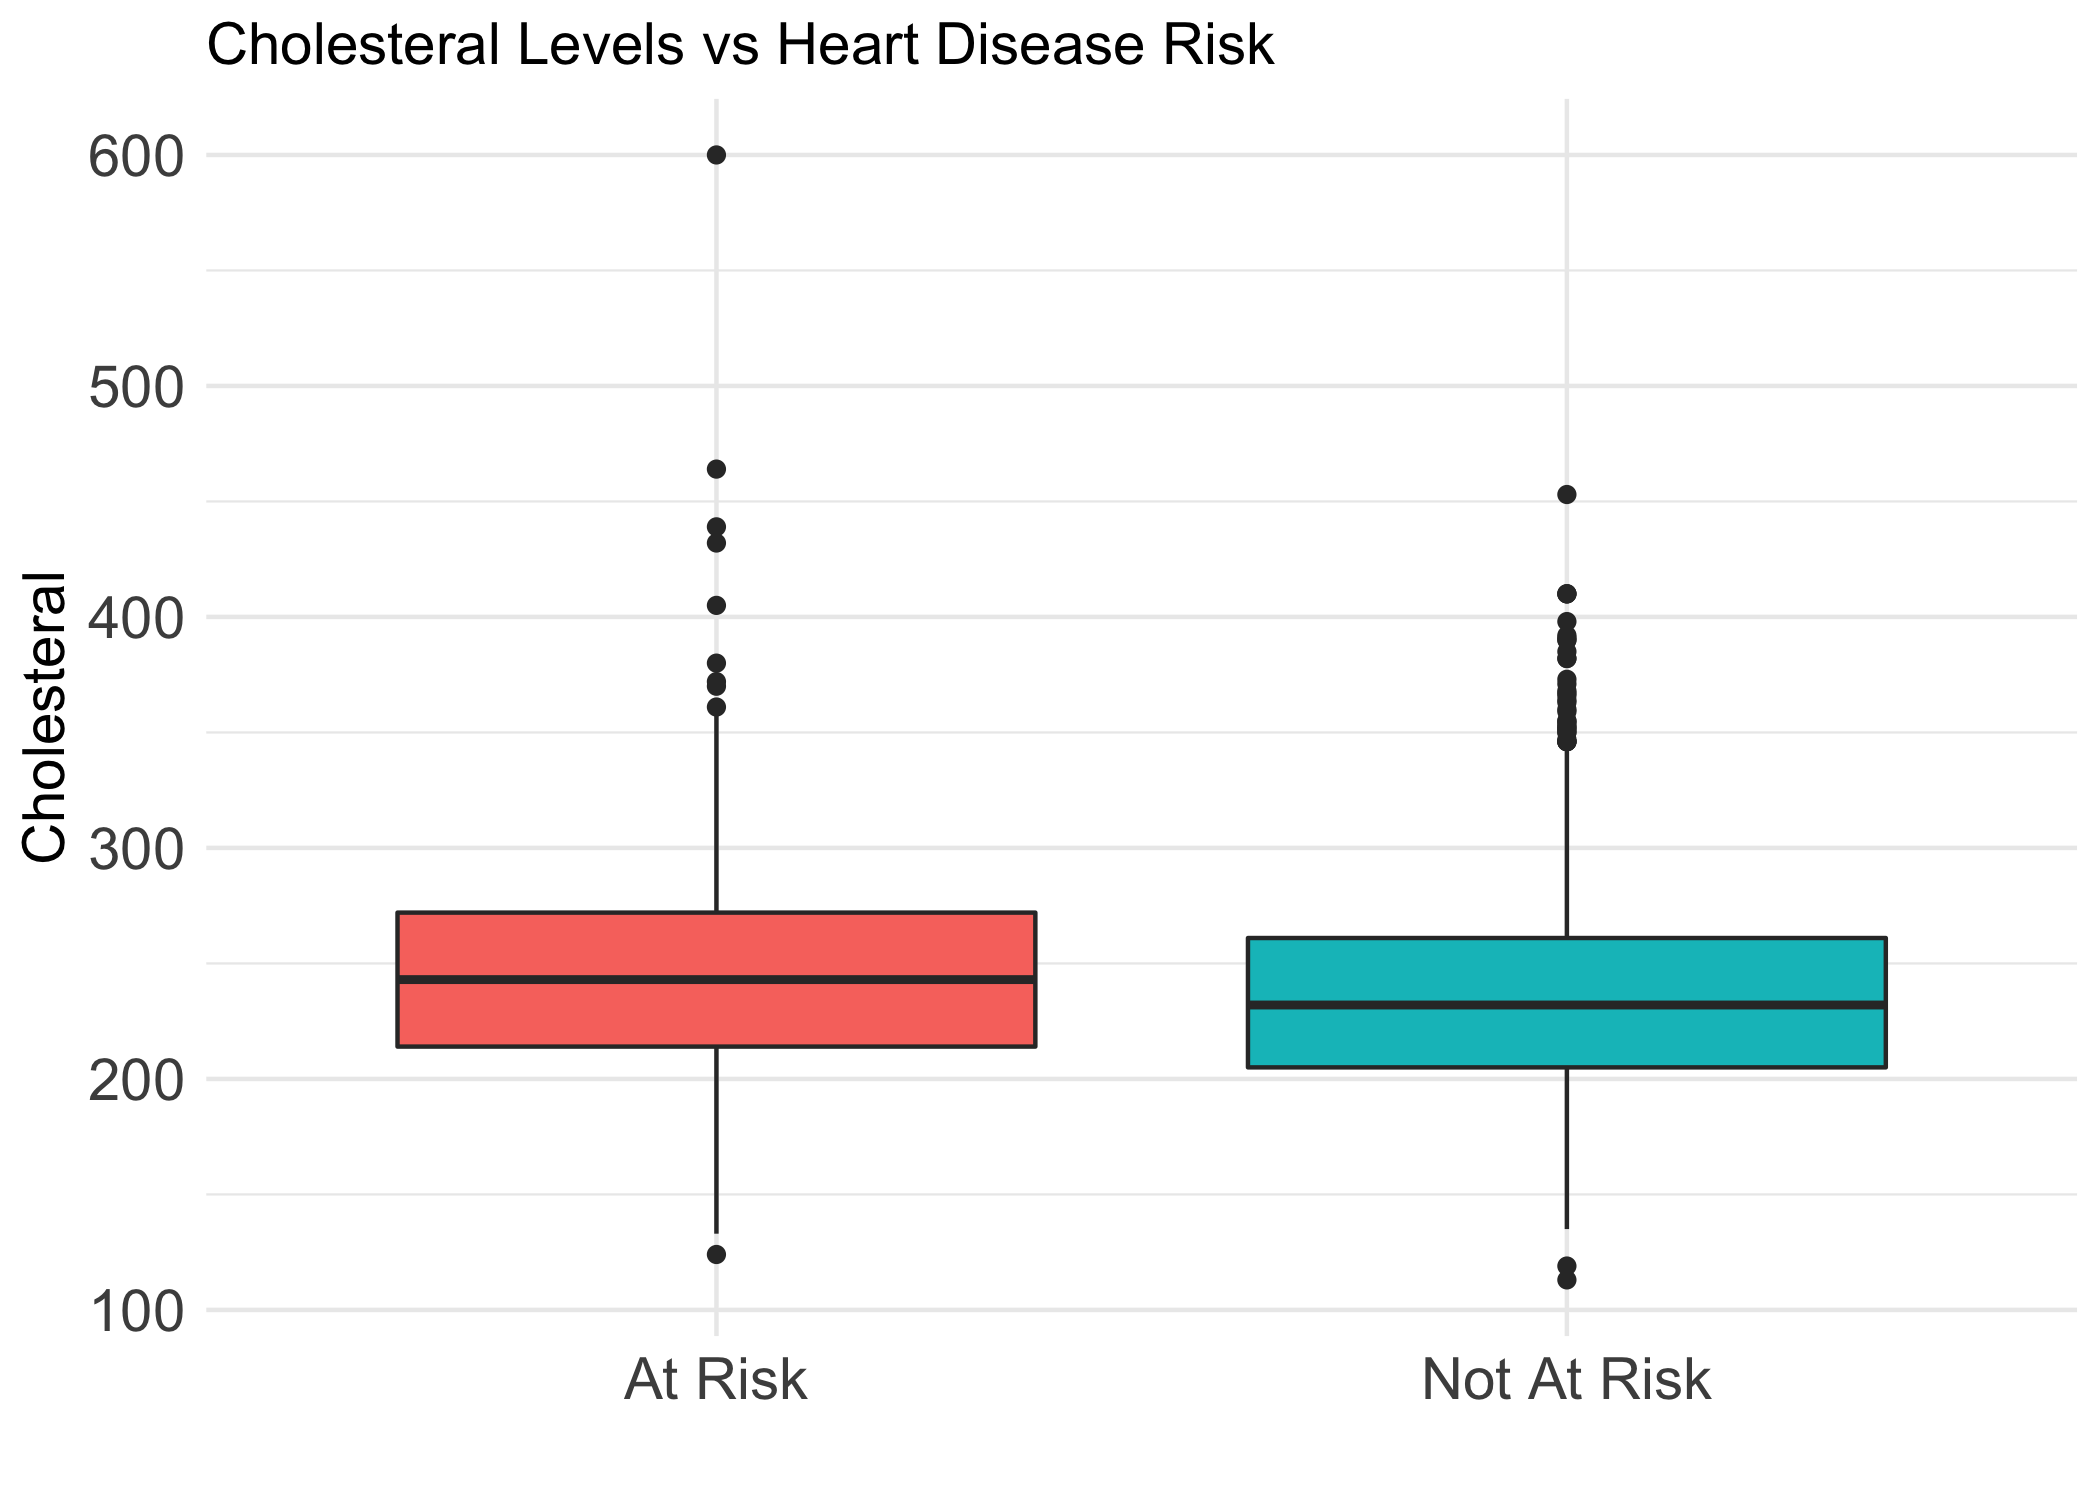
\includegraphics[height=45mm, width=65mm]{box_cholesterol.png}}%
\hspace*{\fill}
\end{figure}



\subsubsection*{Systolic Blood Pressure}

The distribution of systolic blood pressure appears approximately normal, centered around 125 mmHg. We can see that an increased level of systolic blood pressure is associated with a larger proportion of patients at risk for 10-year coronary heart disease. 

\begin{figure}[hbt!]
\hspace*{\fill}
\centering
\subcaptionbox*{}{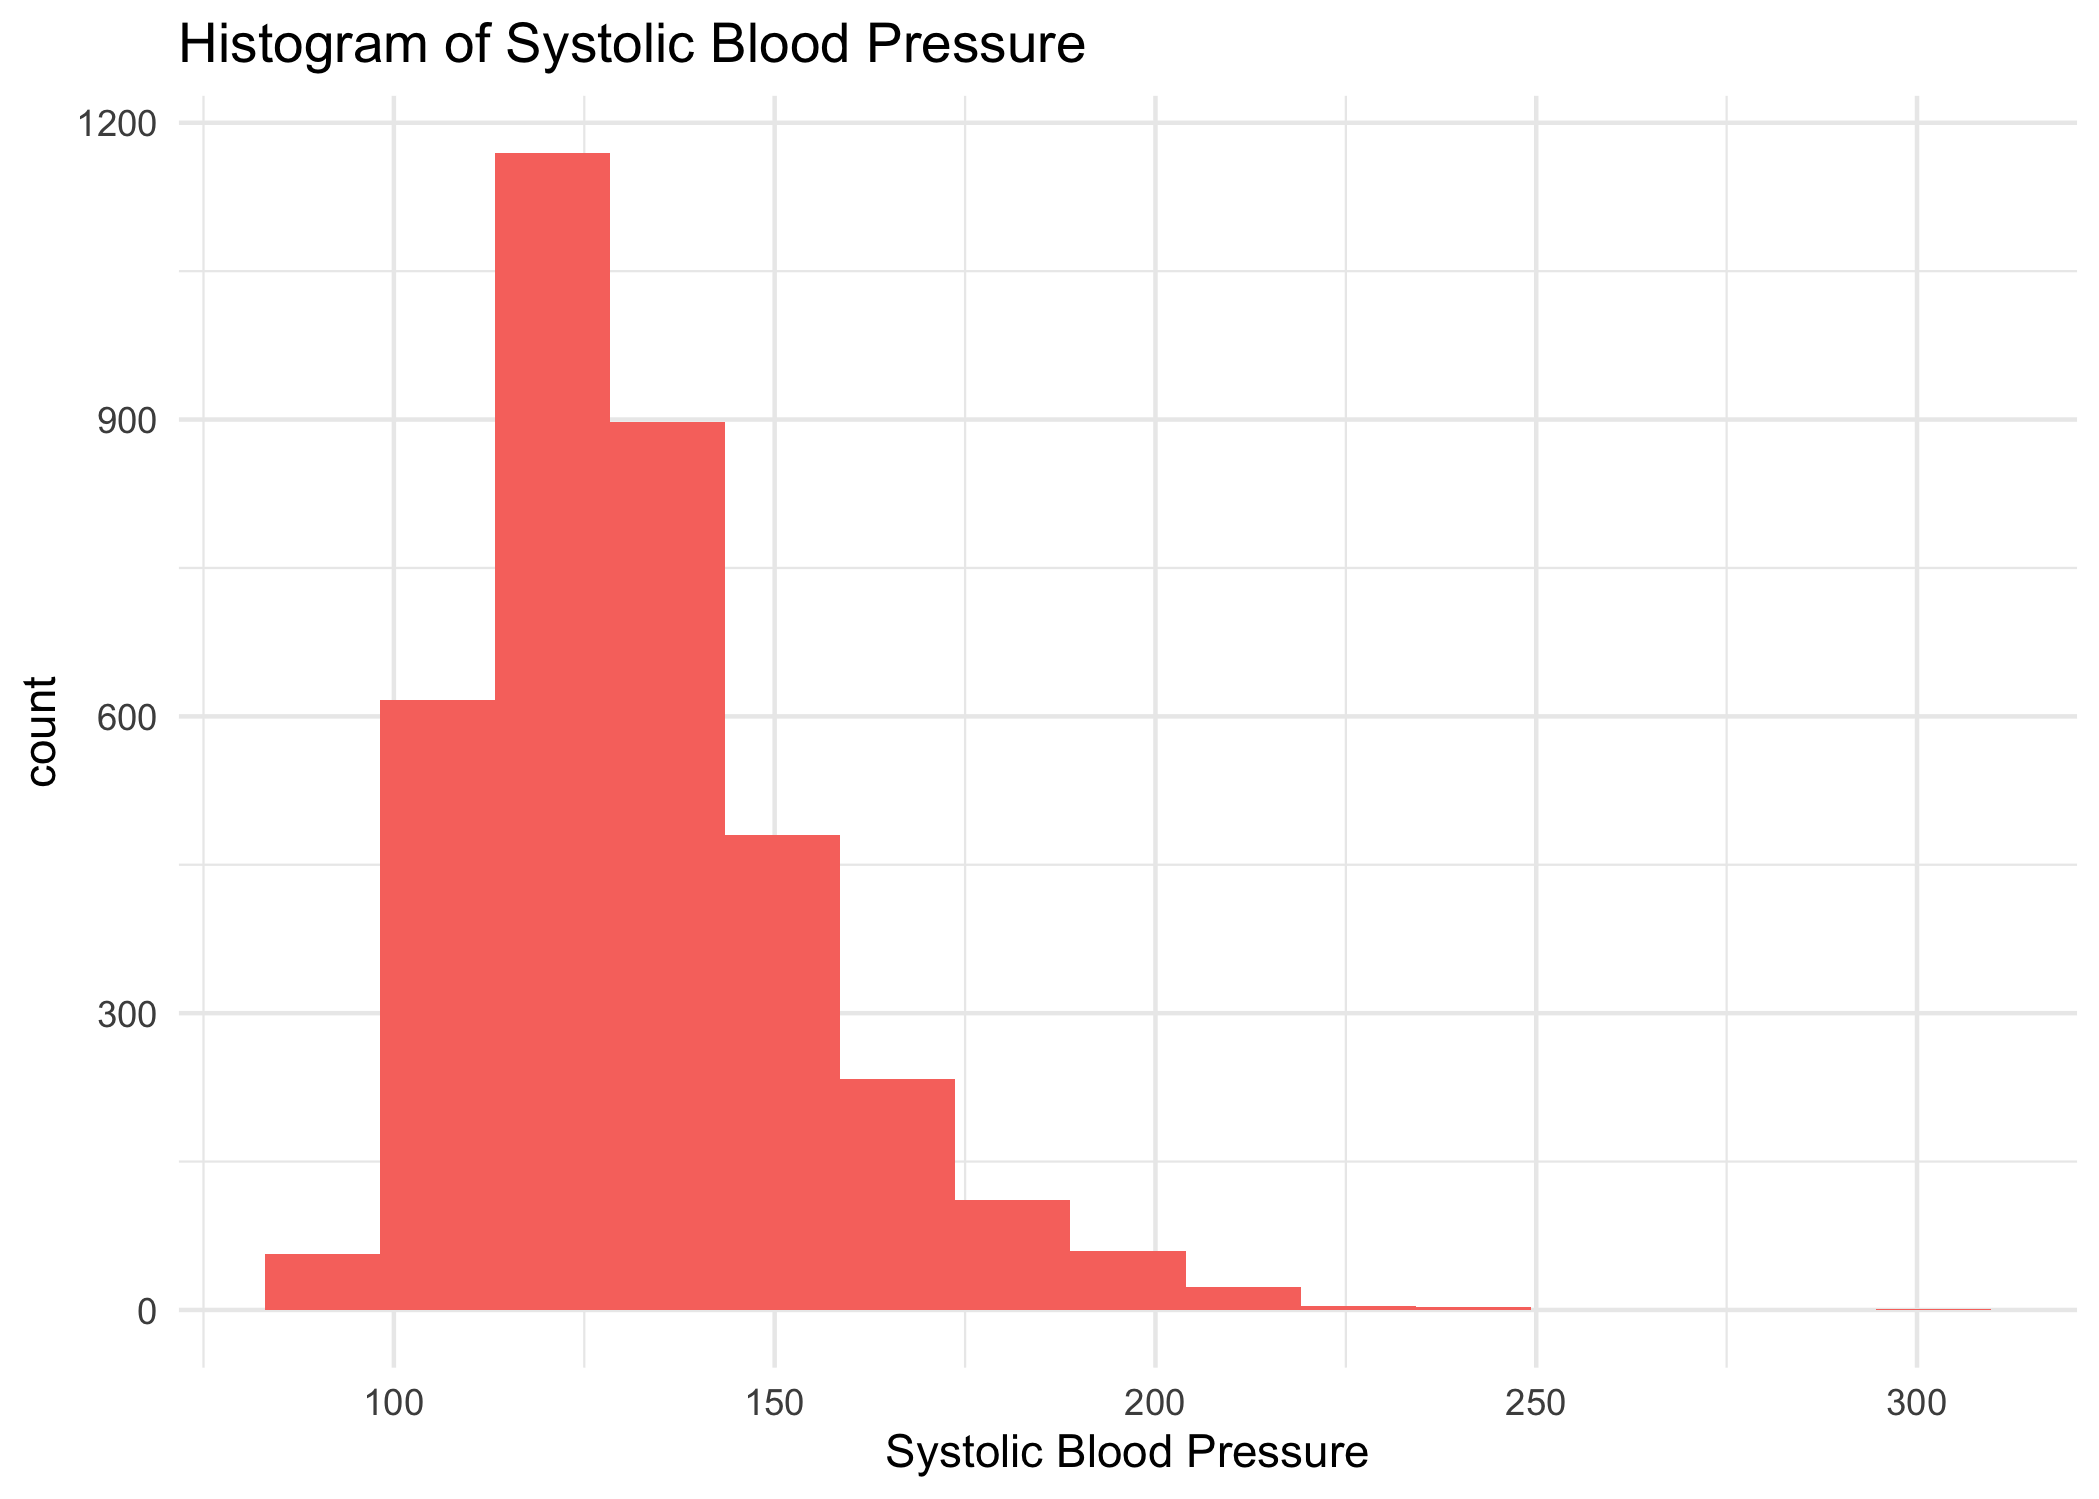
\includegraphics[height=45mm, width=65mm]{hist_sbp.png}}\hspace{2em}%
\subcaptionbox*{}{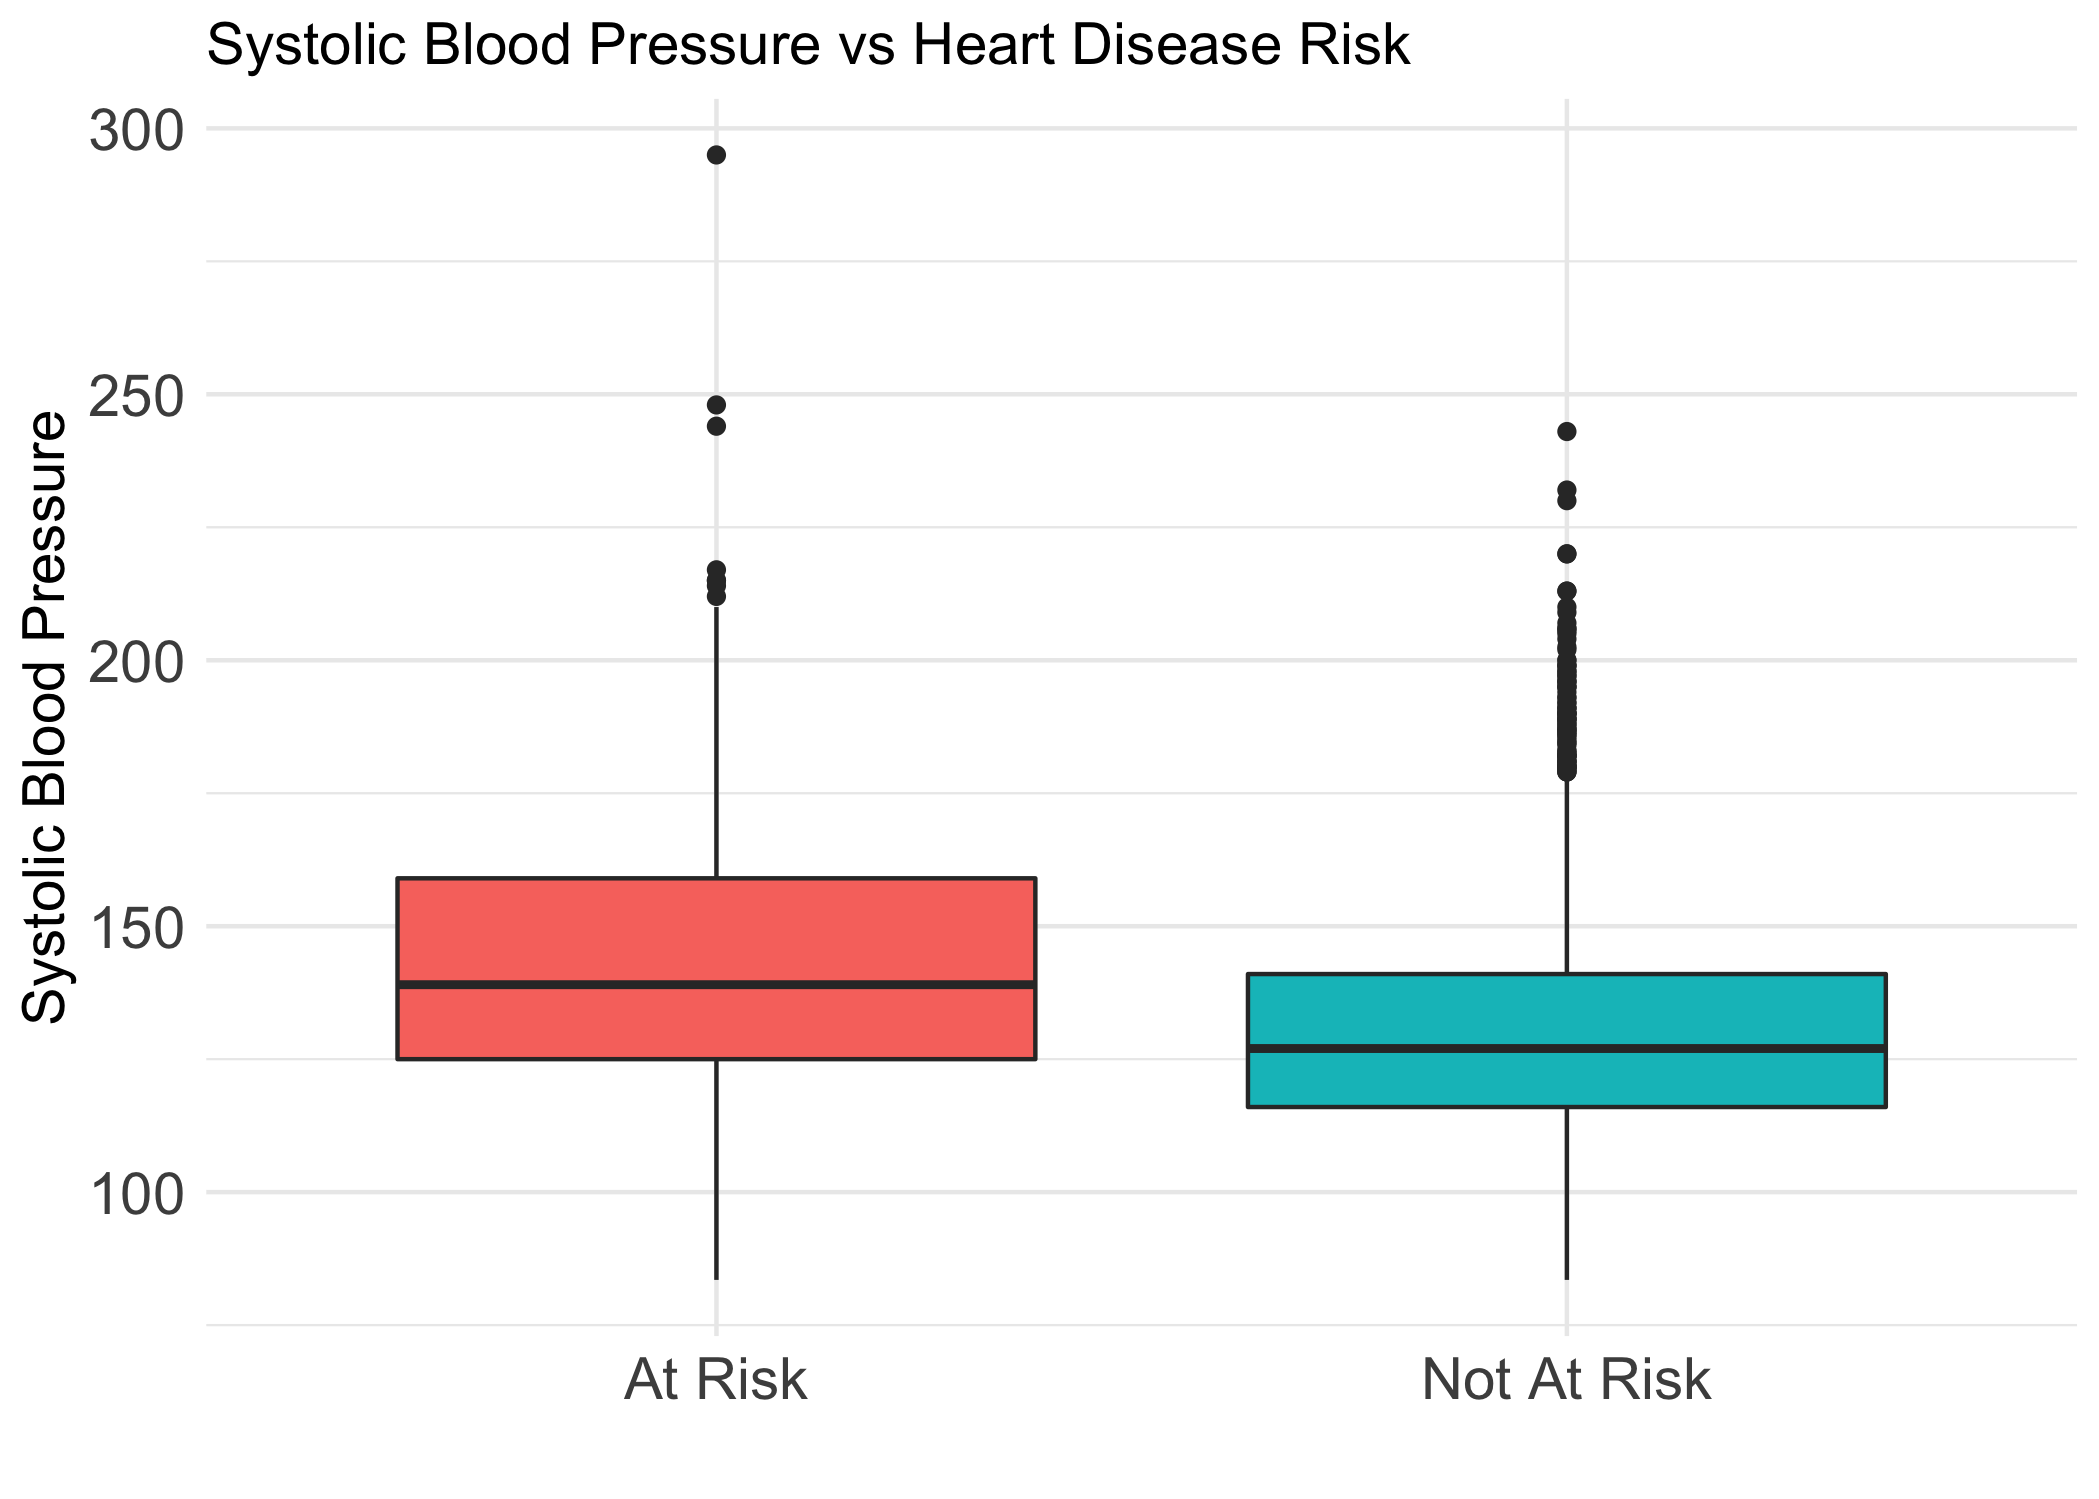
\includegraphics[height=45mm, width=65mm]{box_sbp.png}}%
\hspace*{\fill}
\end{figure}


\subsubsection*{Diastolic Blood Pressure}

As expected, the distribution of diastolic blood pressure also appears approximately normal, centered around 85 mmHg. Notice that the trend continues as before - an increased level of the diastolic blood pressure is associated with a larger proportion of patients at risk for 10-year coronary heart disease.

\begin{figure}[hbt!]
\hspace*{\fill}
\centering
\subcaptionbox*{}{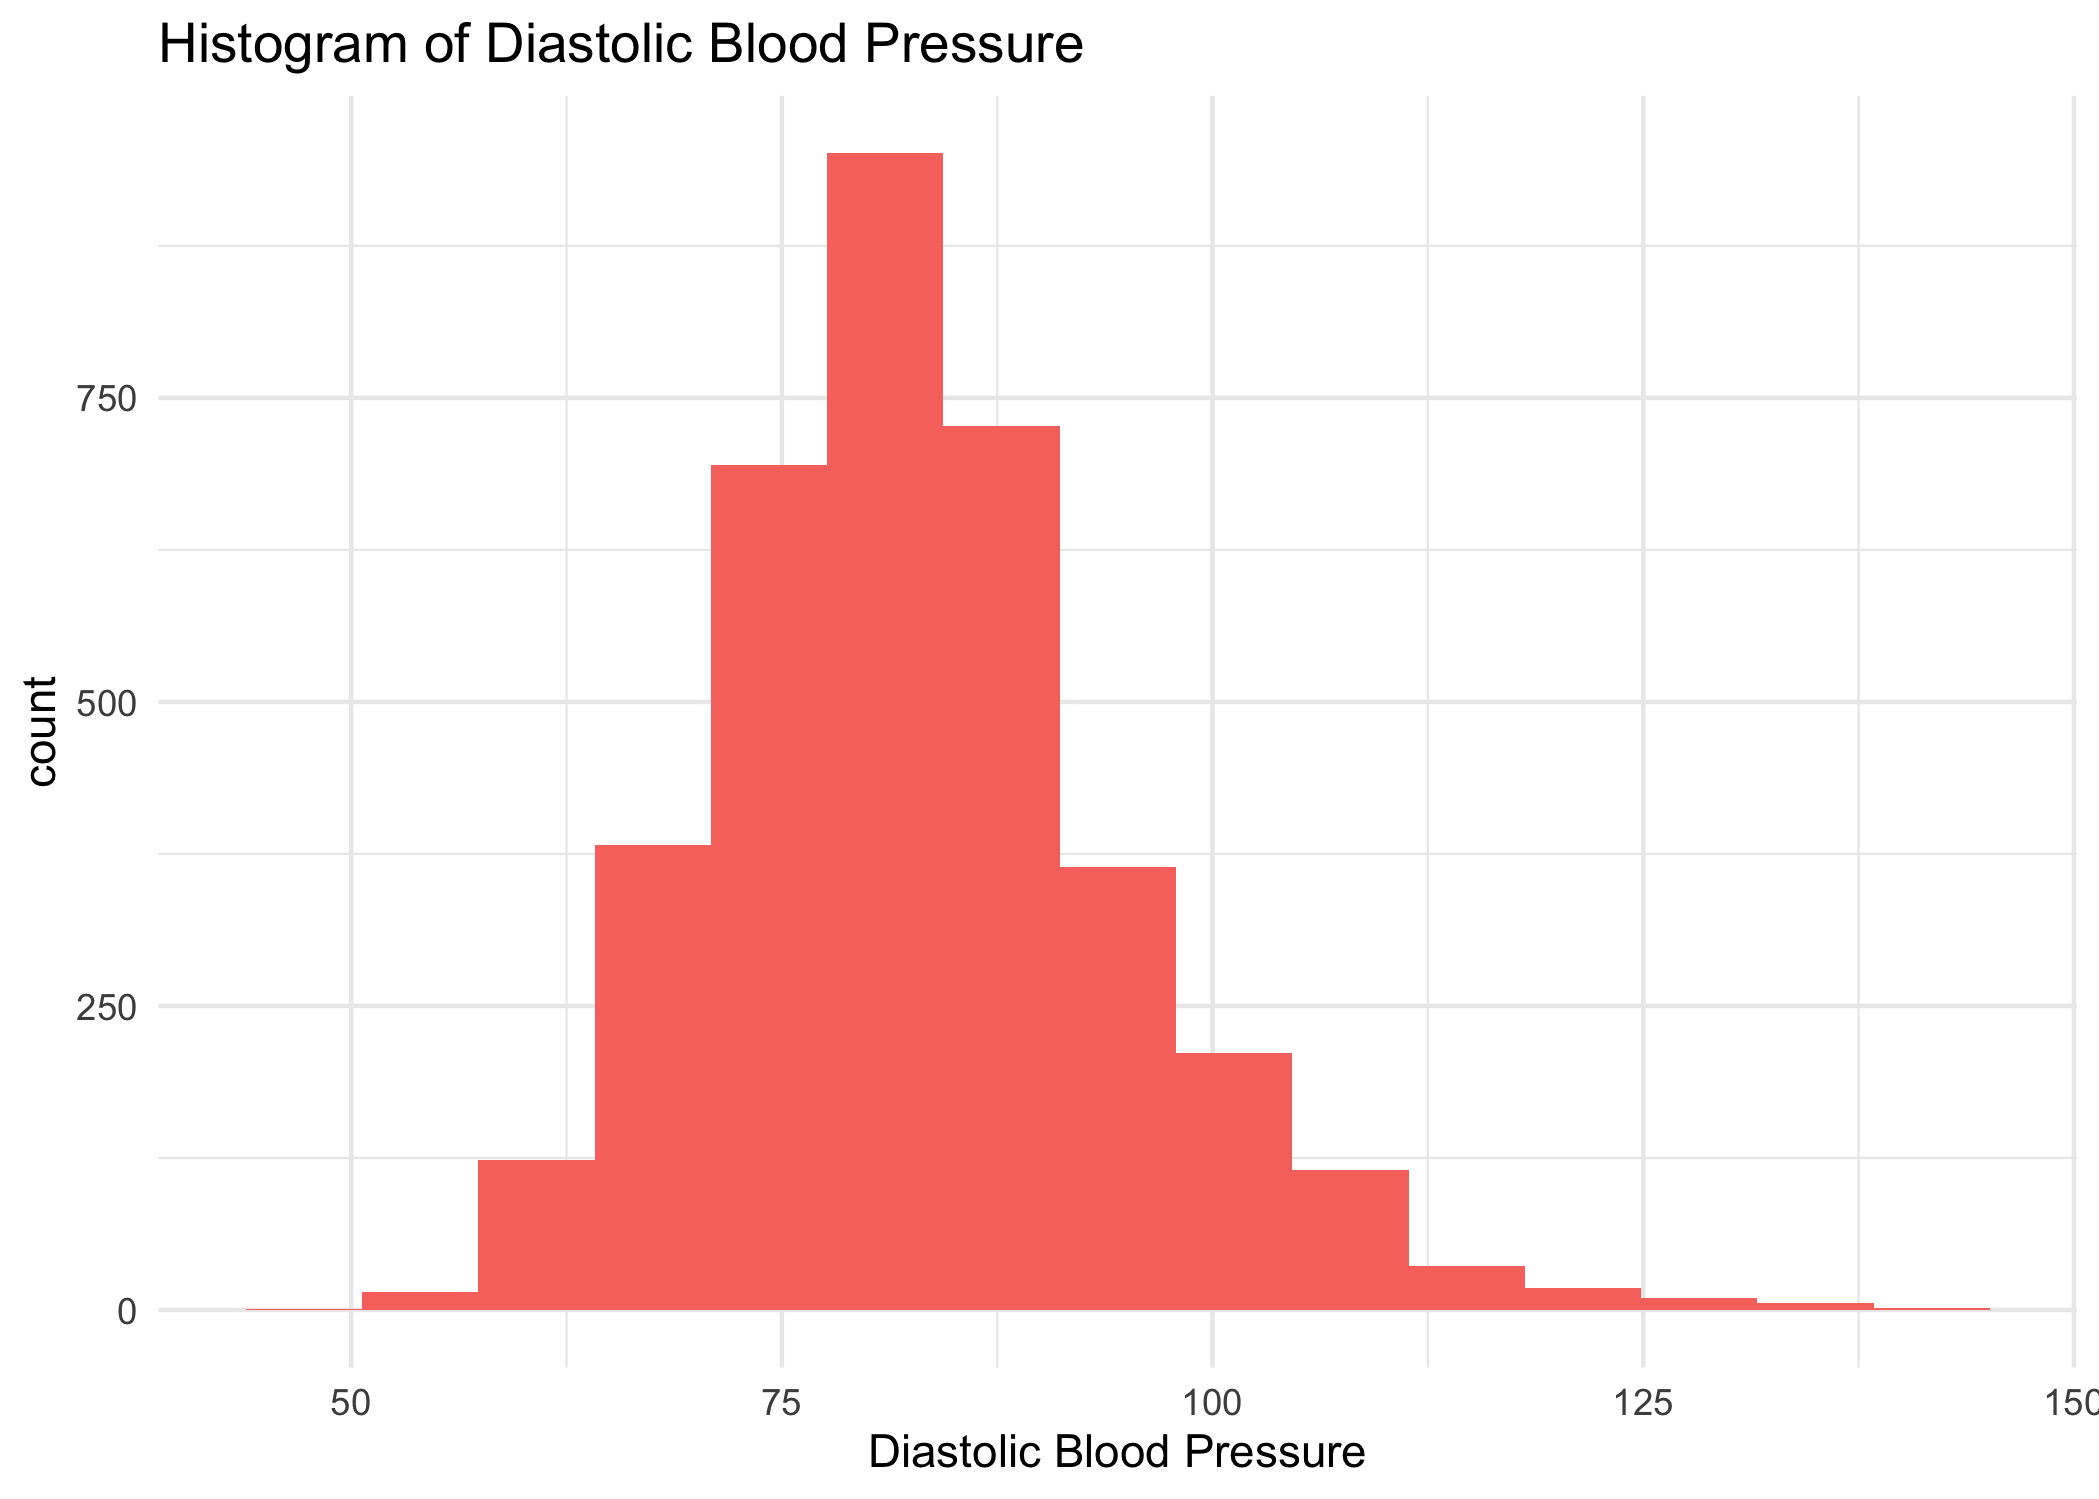
\includegraphics[height=45mm, width=65mm]{hist_dbp.png}}\hspace{2em}%
\subcaptionbox*{}{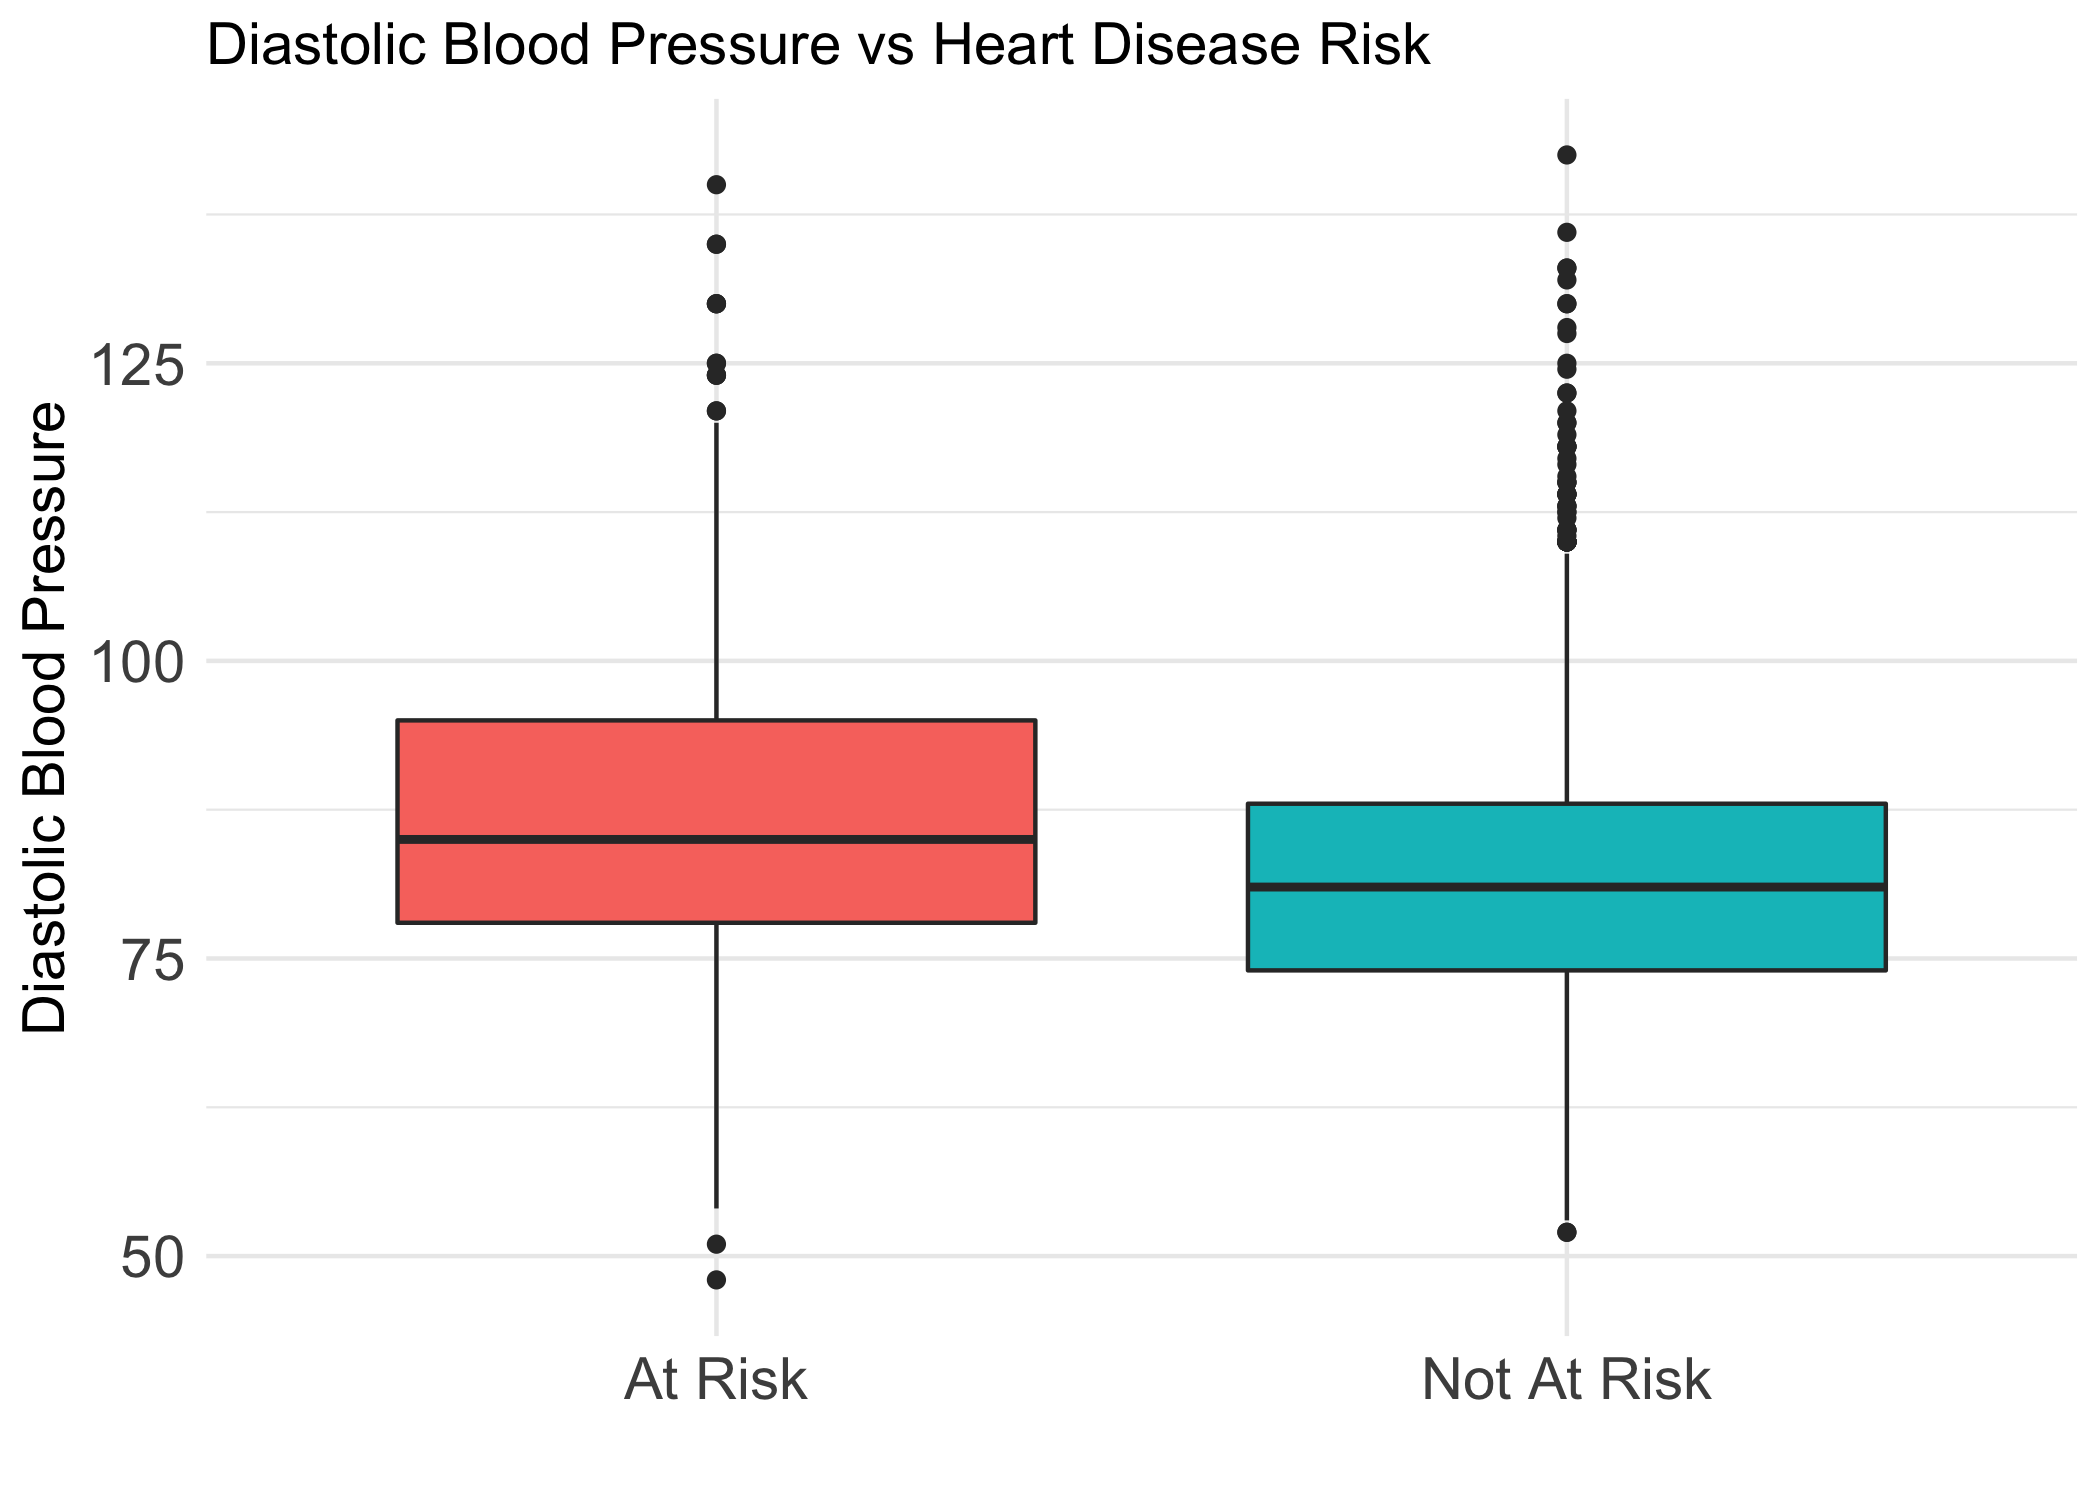
\includegraphics[height=45mm, width=65mm]{box_dbp.png}}%
\hspace*{\fill}
\end{figure}


\subsubsection*{Body Mass Index}

The majority of patients in our study are either at a healthy weight or overweight. Very few patients are underweight in the dataset. Despite the unequal number of patients per group, the proportion of patients at risk for 10-year coronary heart disease is approximately equal across groups. 

\begin{figure}[hbt!]
\hspace*{\fill}
\centering
\subcaptionbox*{}{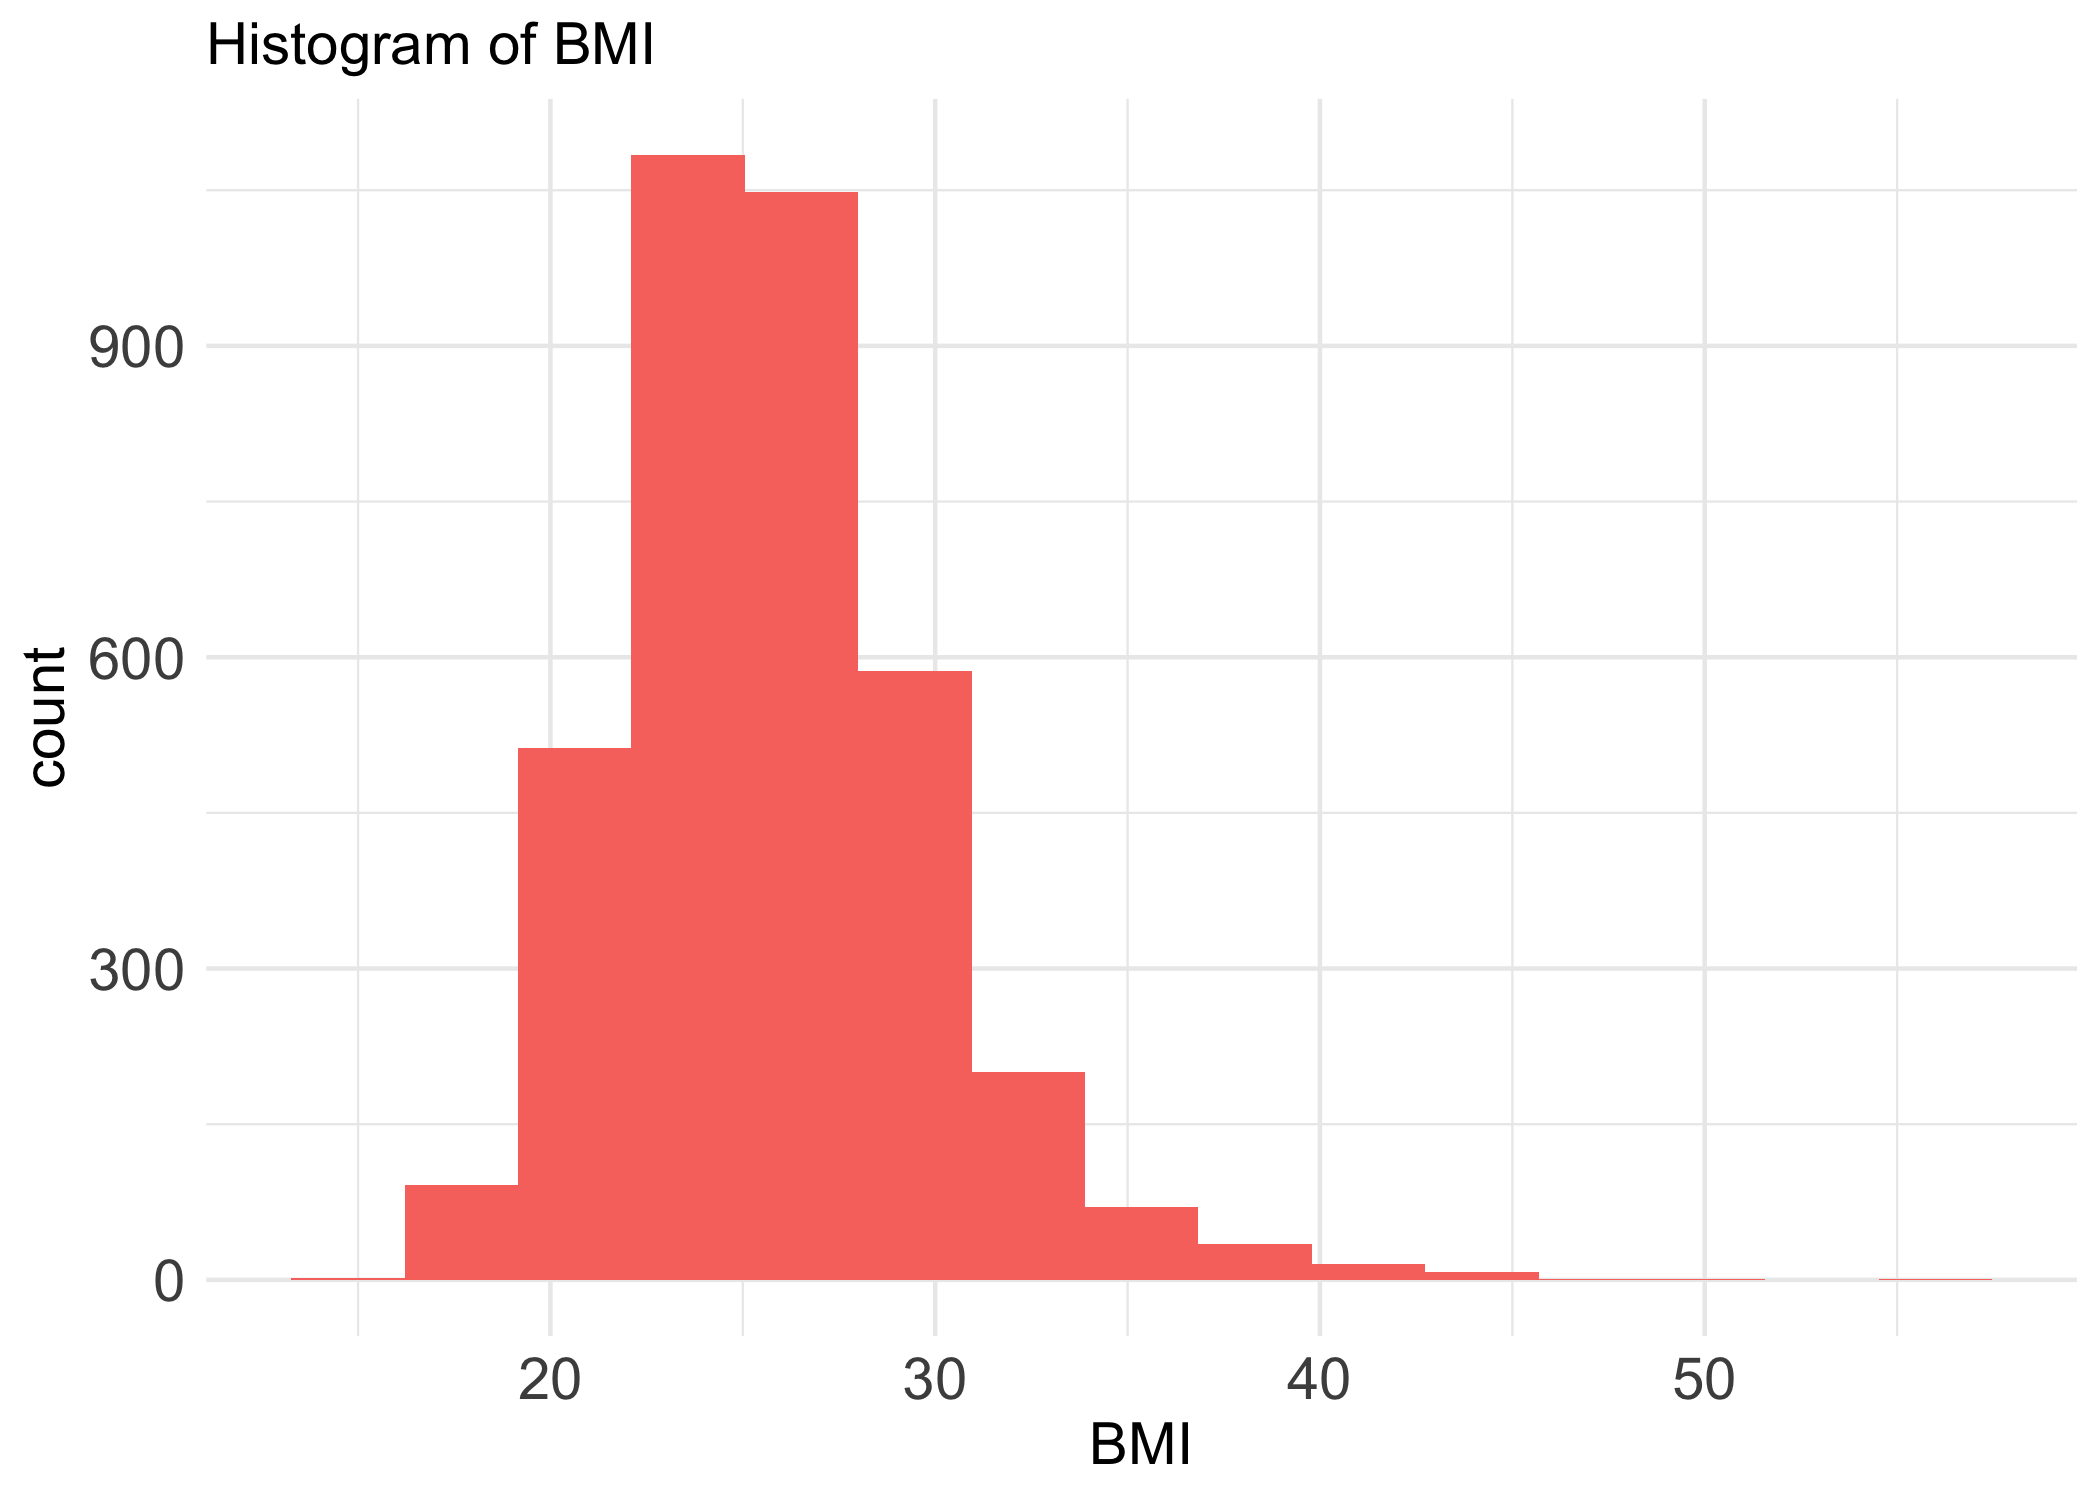
\includegraphics[height=45mm, width=65mm]{hist_bmi.png}}\hspace{2em}%
\subcaptionbox*{}{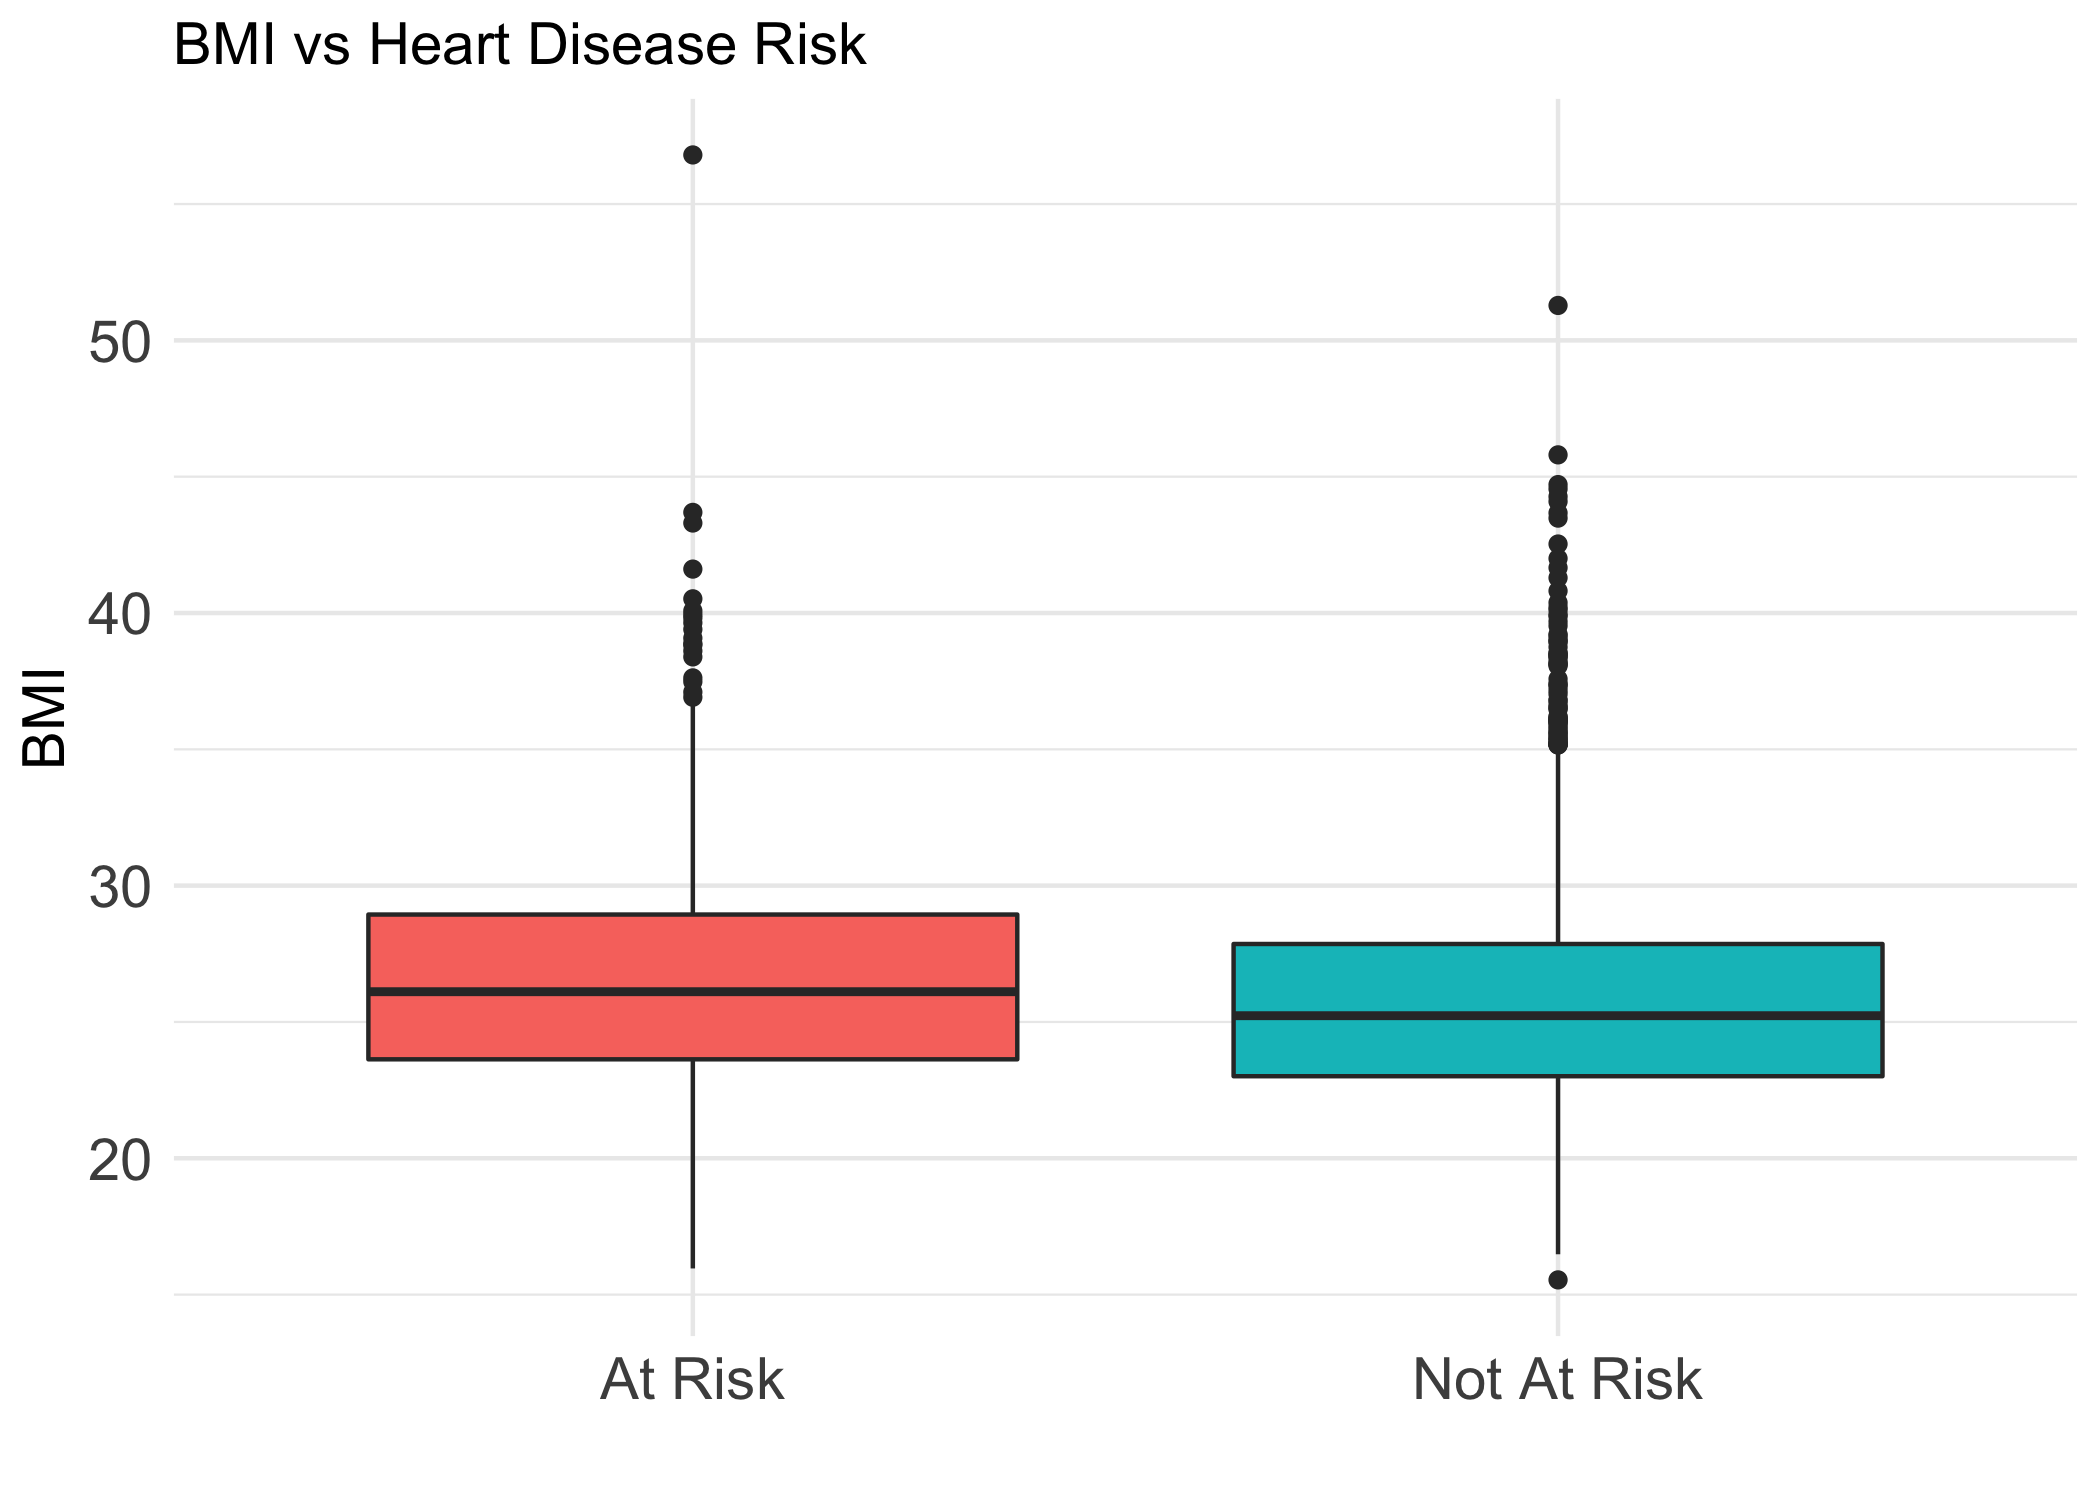
\includegraphics[height=45mm, width=65mm]{box_bmi.png}}%
\hspace*{\fill}
\end{figure}

\subsubsection*{Heart Rate}

According to the histogram below, patients' heart rates are approximately normally distributed. The average patient heart rate is 75 bpm and the standard deviation is 12 bpm. The distribution of patients' heart rates at risk for 10-year coronary heart disease is nearly identical to the distribution of patients' heart rates not at risk for 10-year coronary heart disease.

\begin{figure}[hbt!]
\hspace*{\fill}
\centering
\subcaptionbox*{}{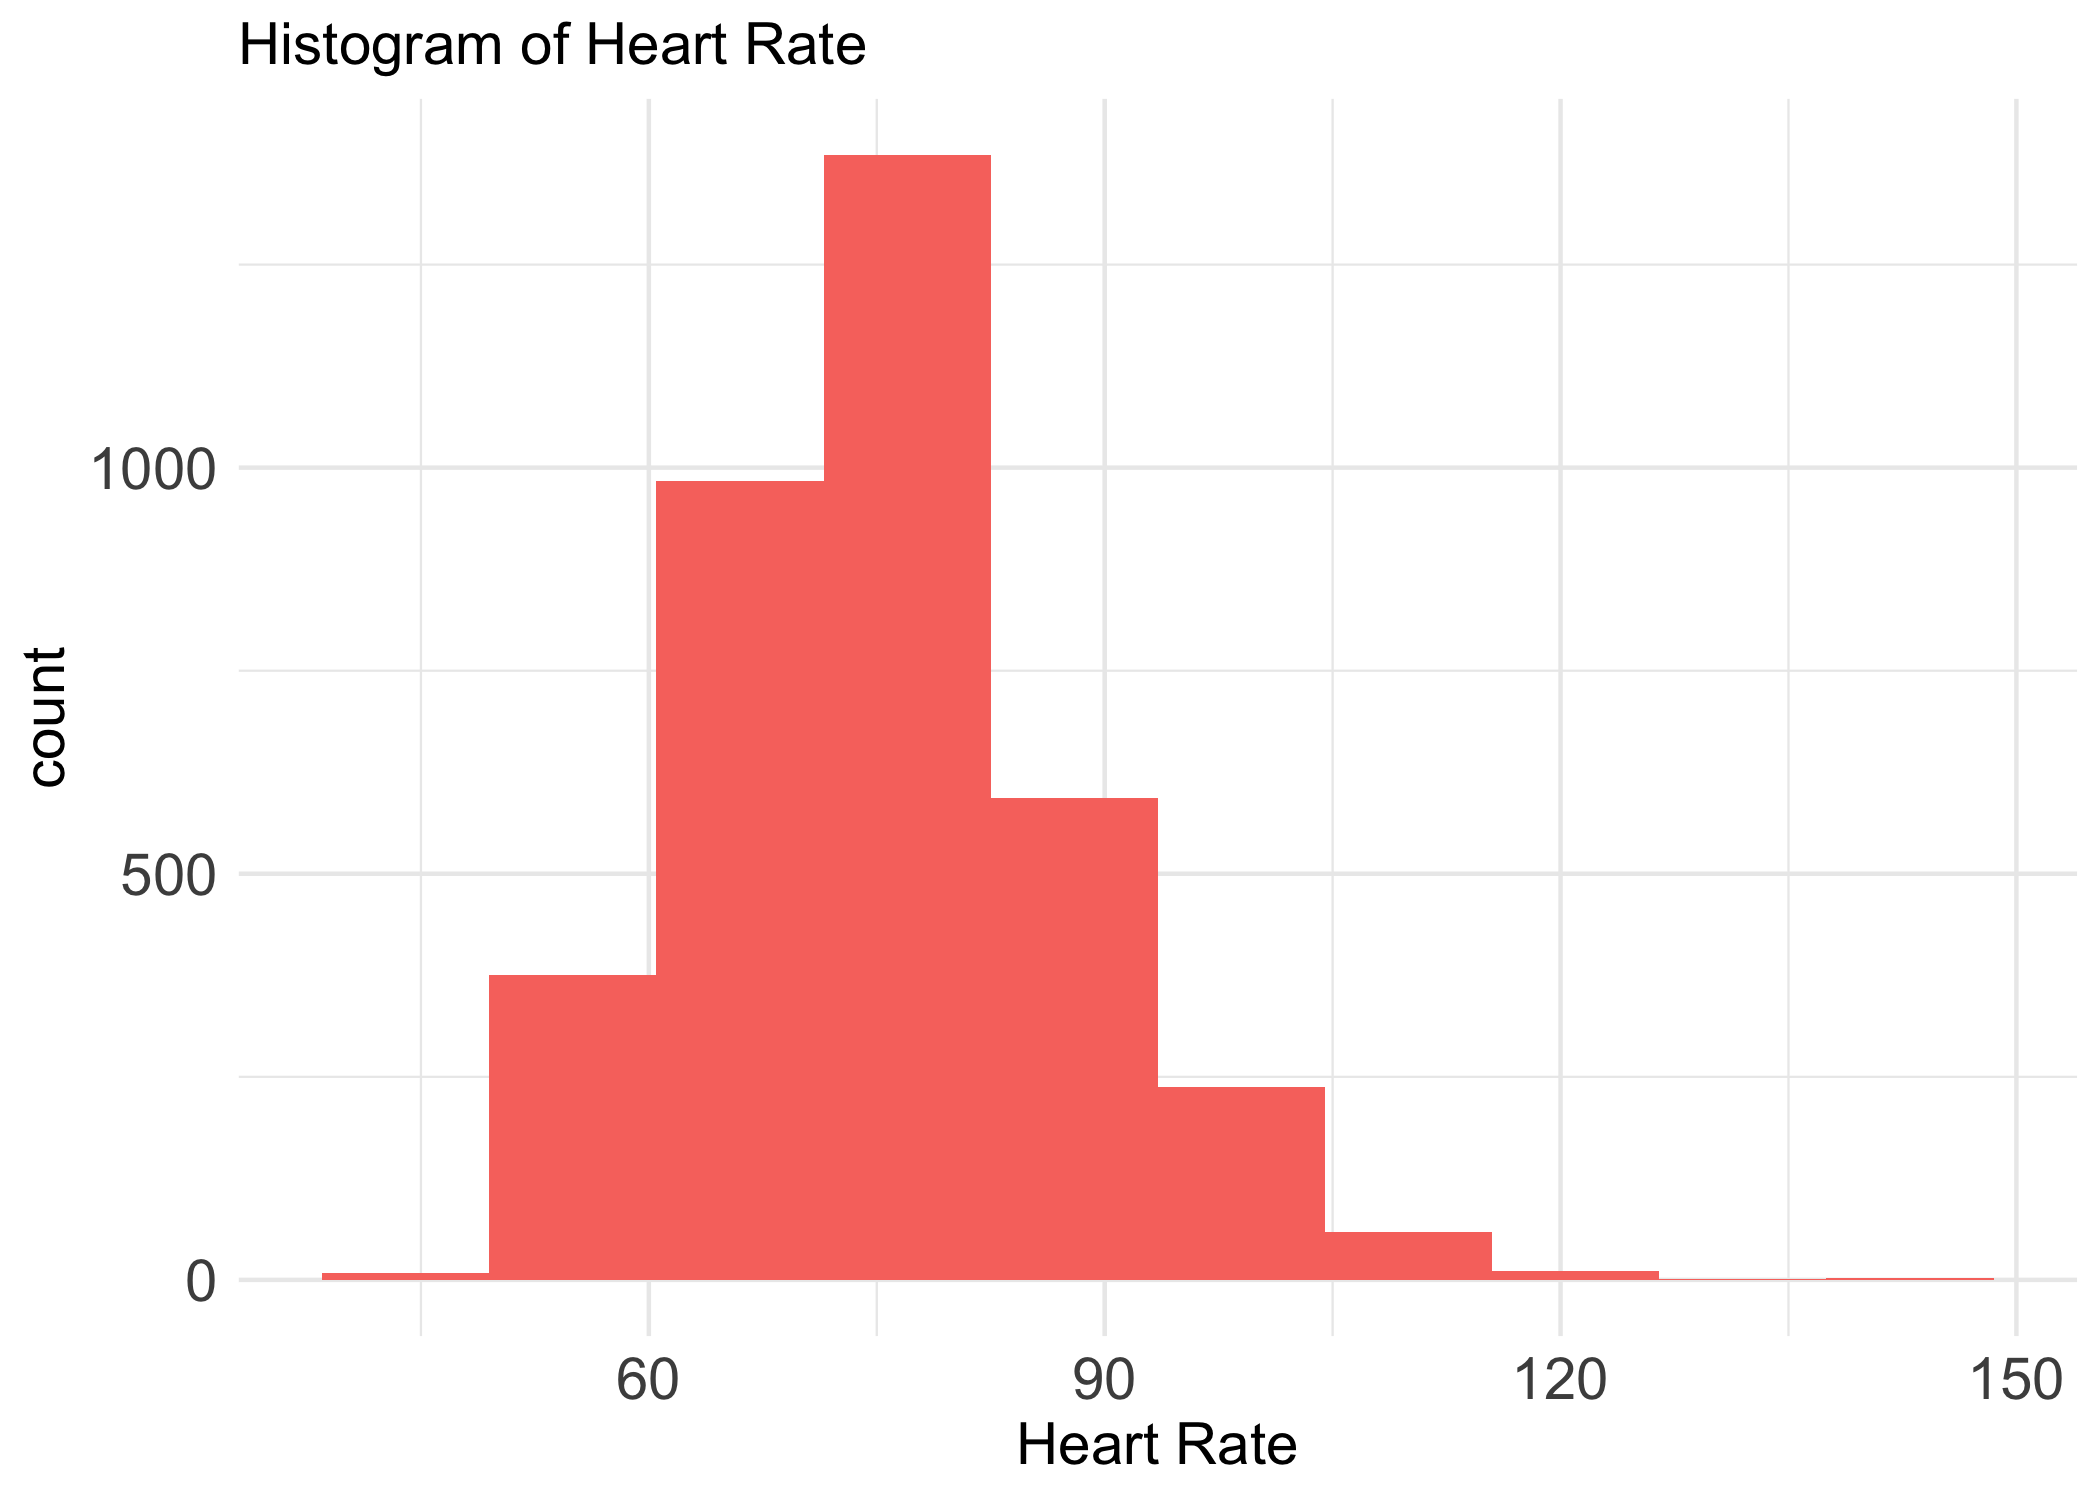
\includegraphics[height=45mm, width=65mm]{hist_heart_rate.png}}\hspace{2em}%
\subcaptionbox*{}{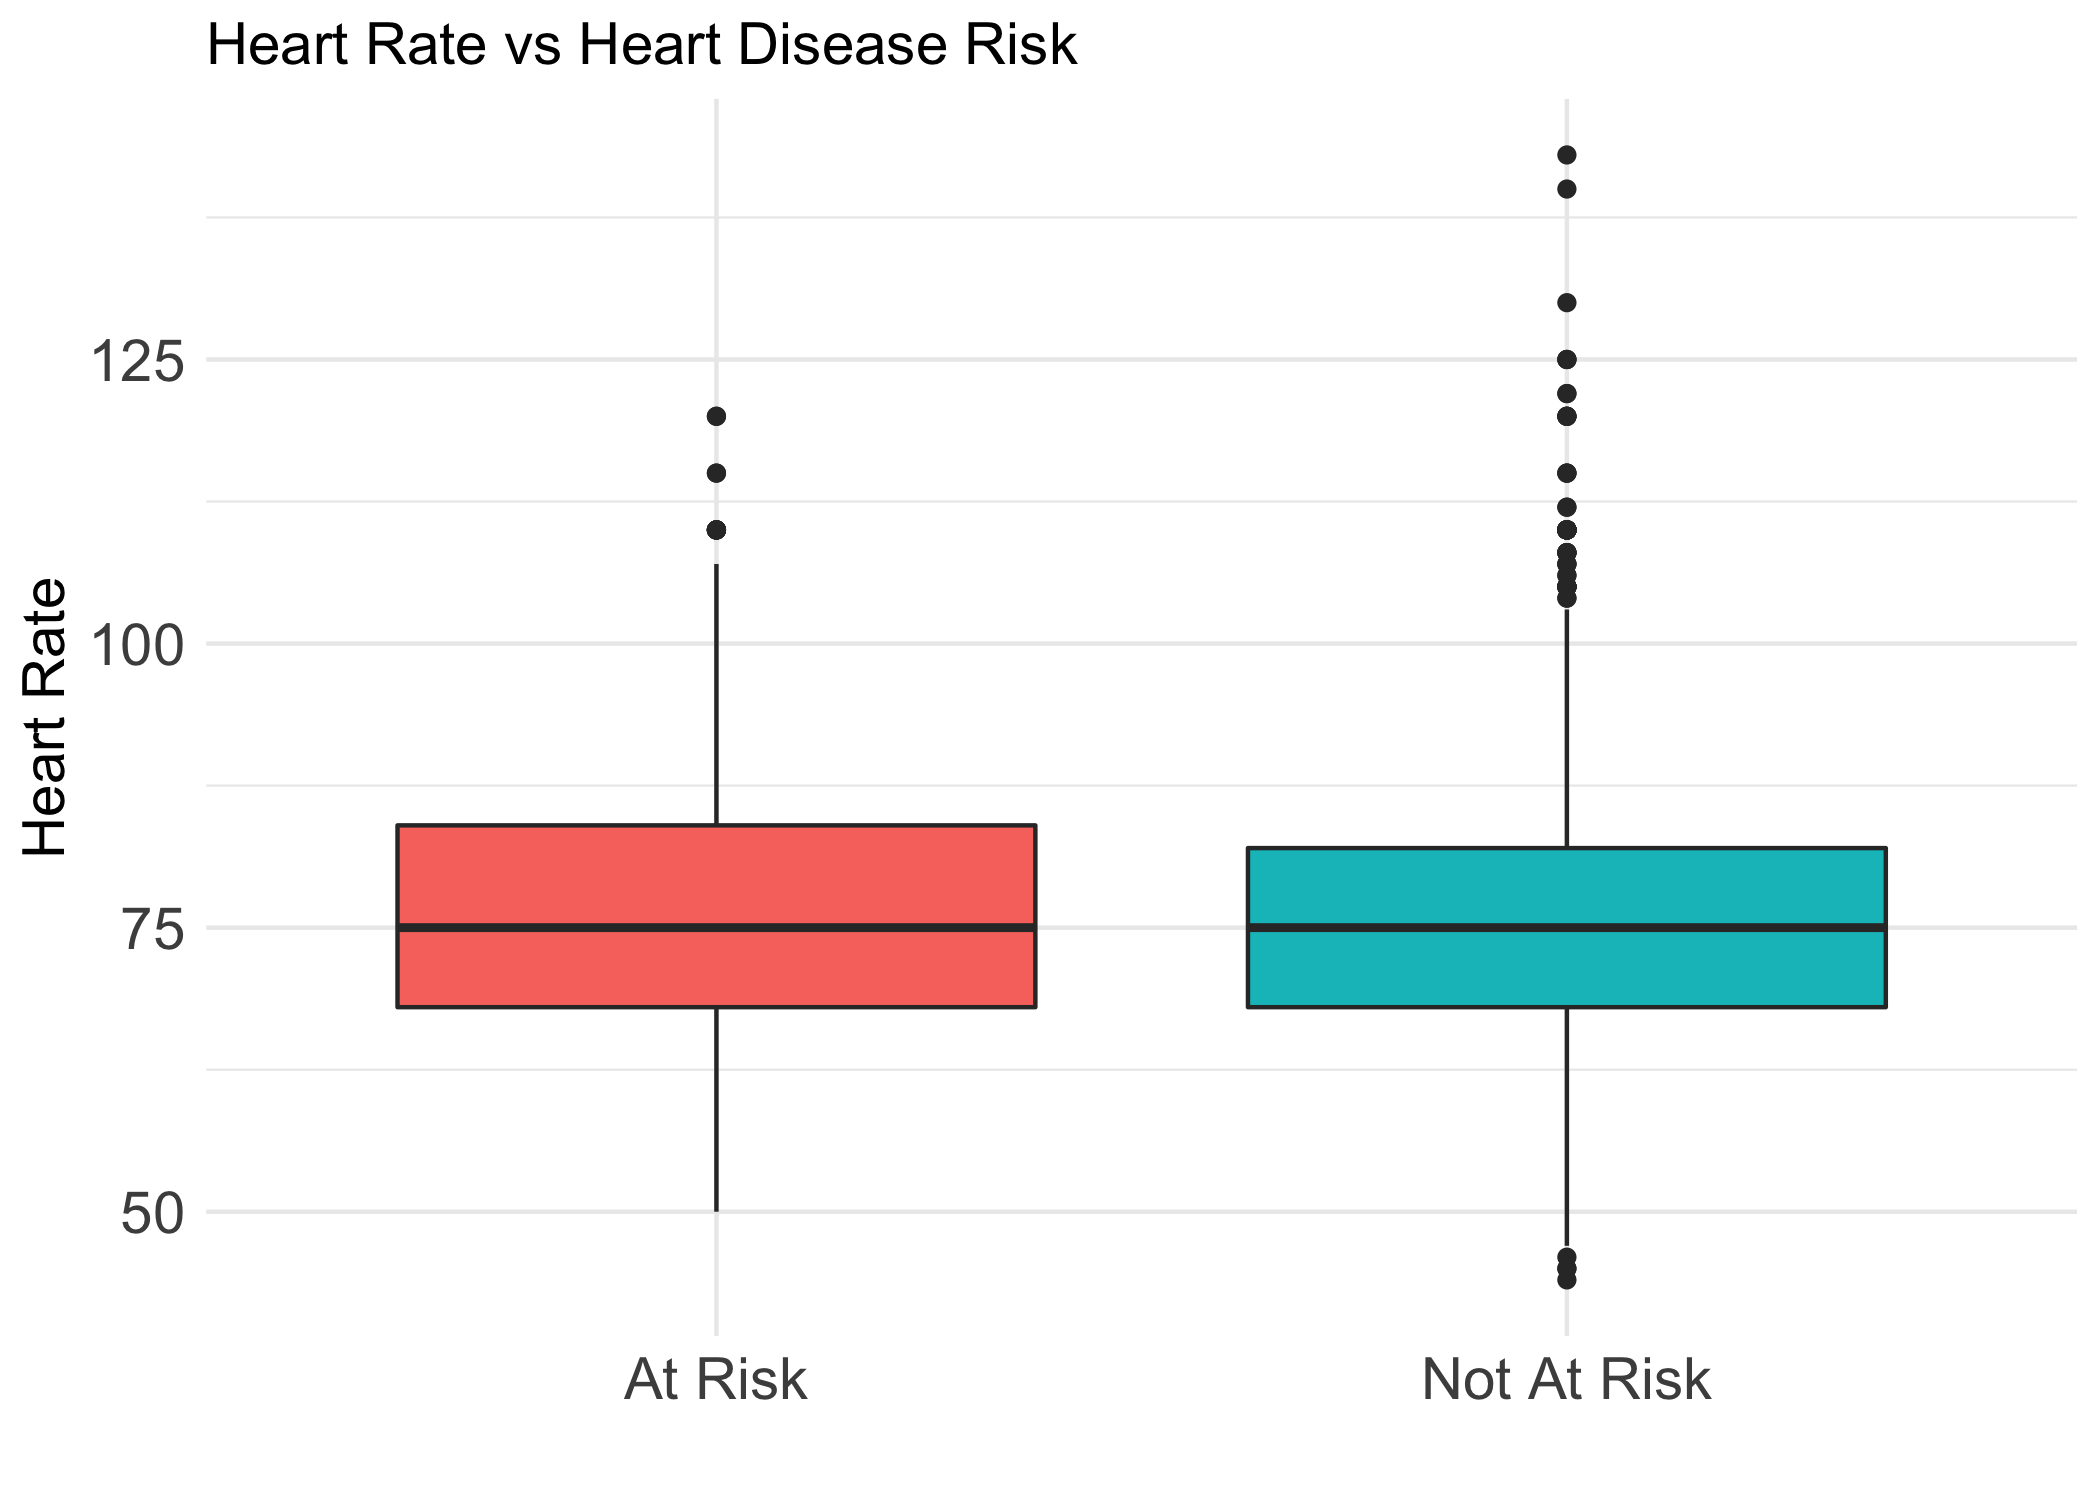
\includegraphics[height=45mm, width=65mm]{box_heart_rate.png}}%
\hspace*{\fill}
\end{figure}


\subsubsection*{Glucose}

Very few patients in the study have a diabetic glucose level. The majority of patients fall in the normal glucose range. However, a little over 15\% of patients in the normal glucose range are at risk for 10-year coronary heart disease. Nearly 25\% of patients in the diabetic glucose level are at risk for 10-year coronary heart disease.

\begin{figure}[hbt!]
\hspace*{\fill}
\centering
\subcaptionbox*{}{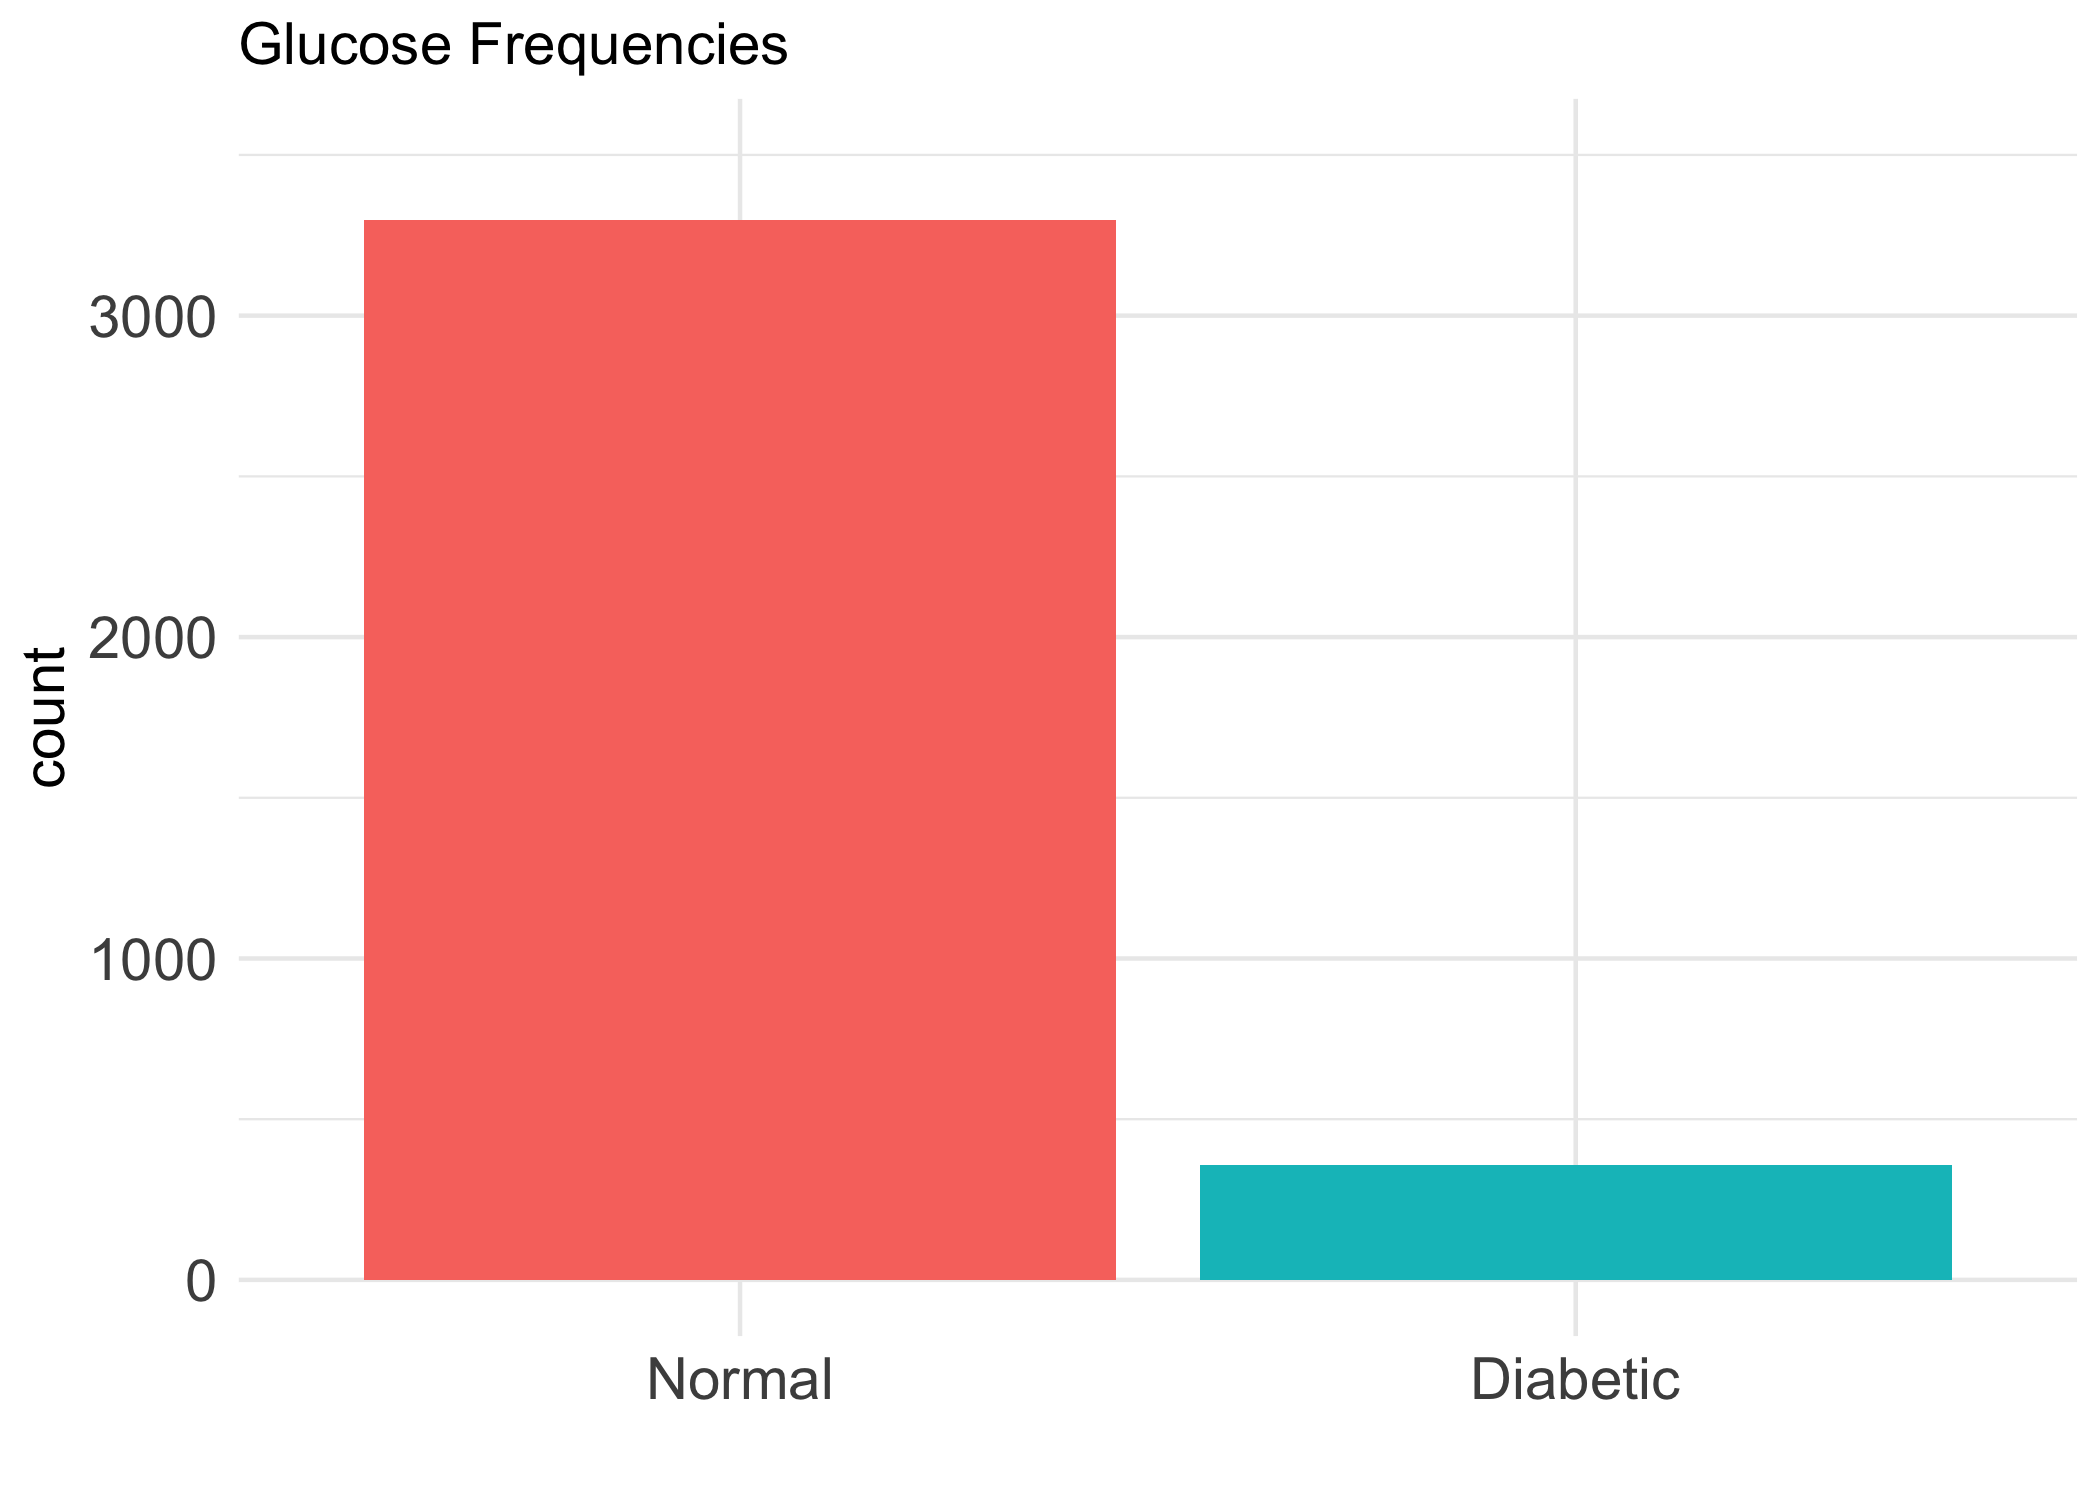
\includegraphics[height=45mm, width=65mm]{bar_glucose.png}}\hspace{2em}%
\subcaptionbox*{}{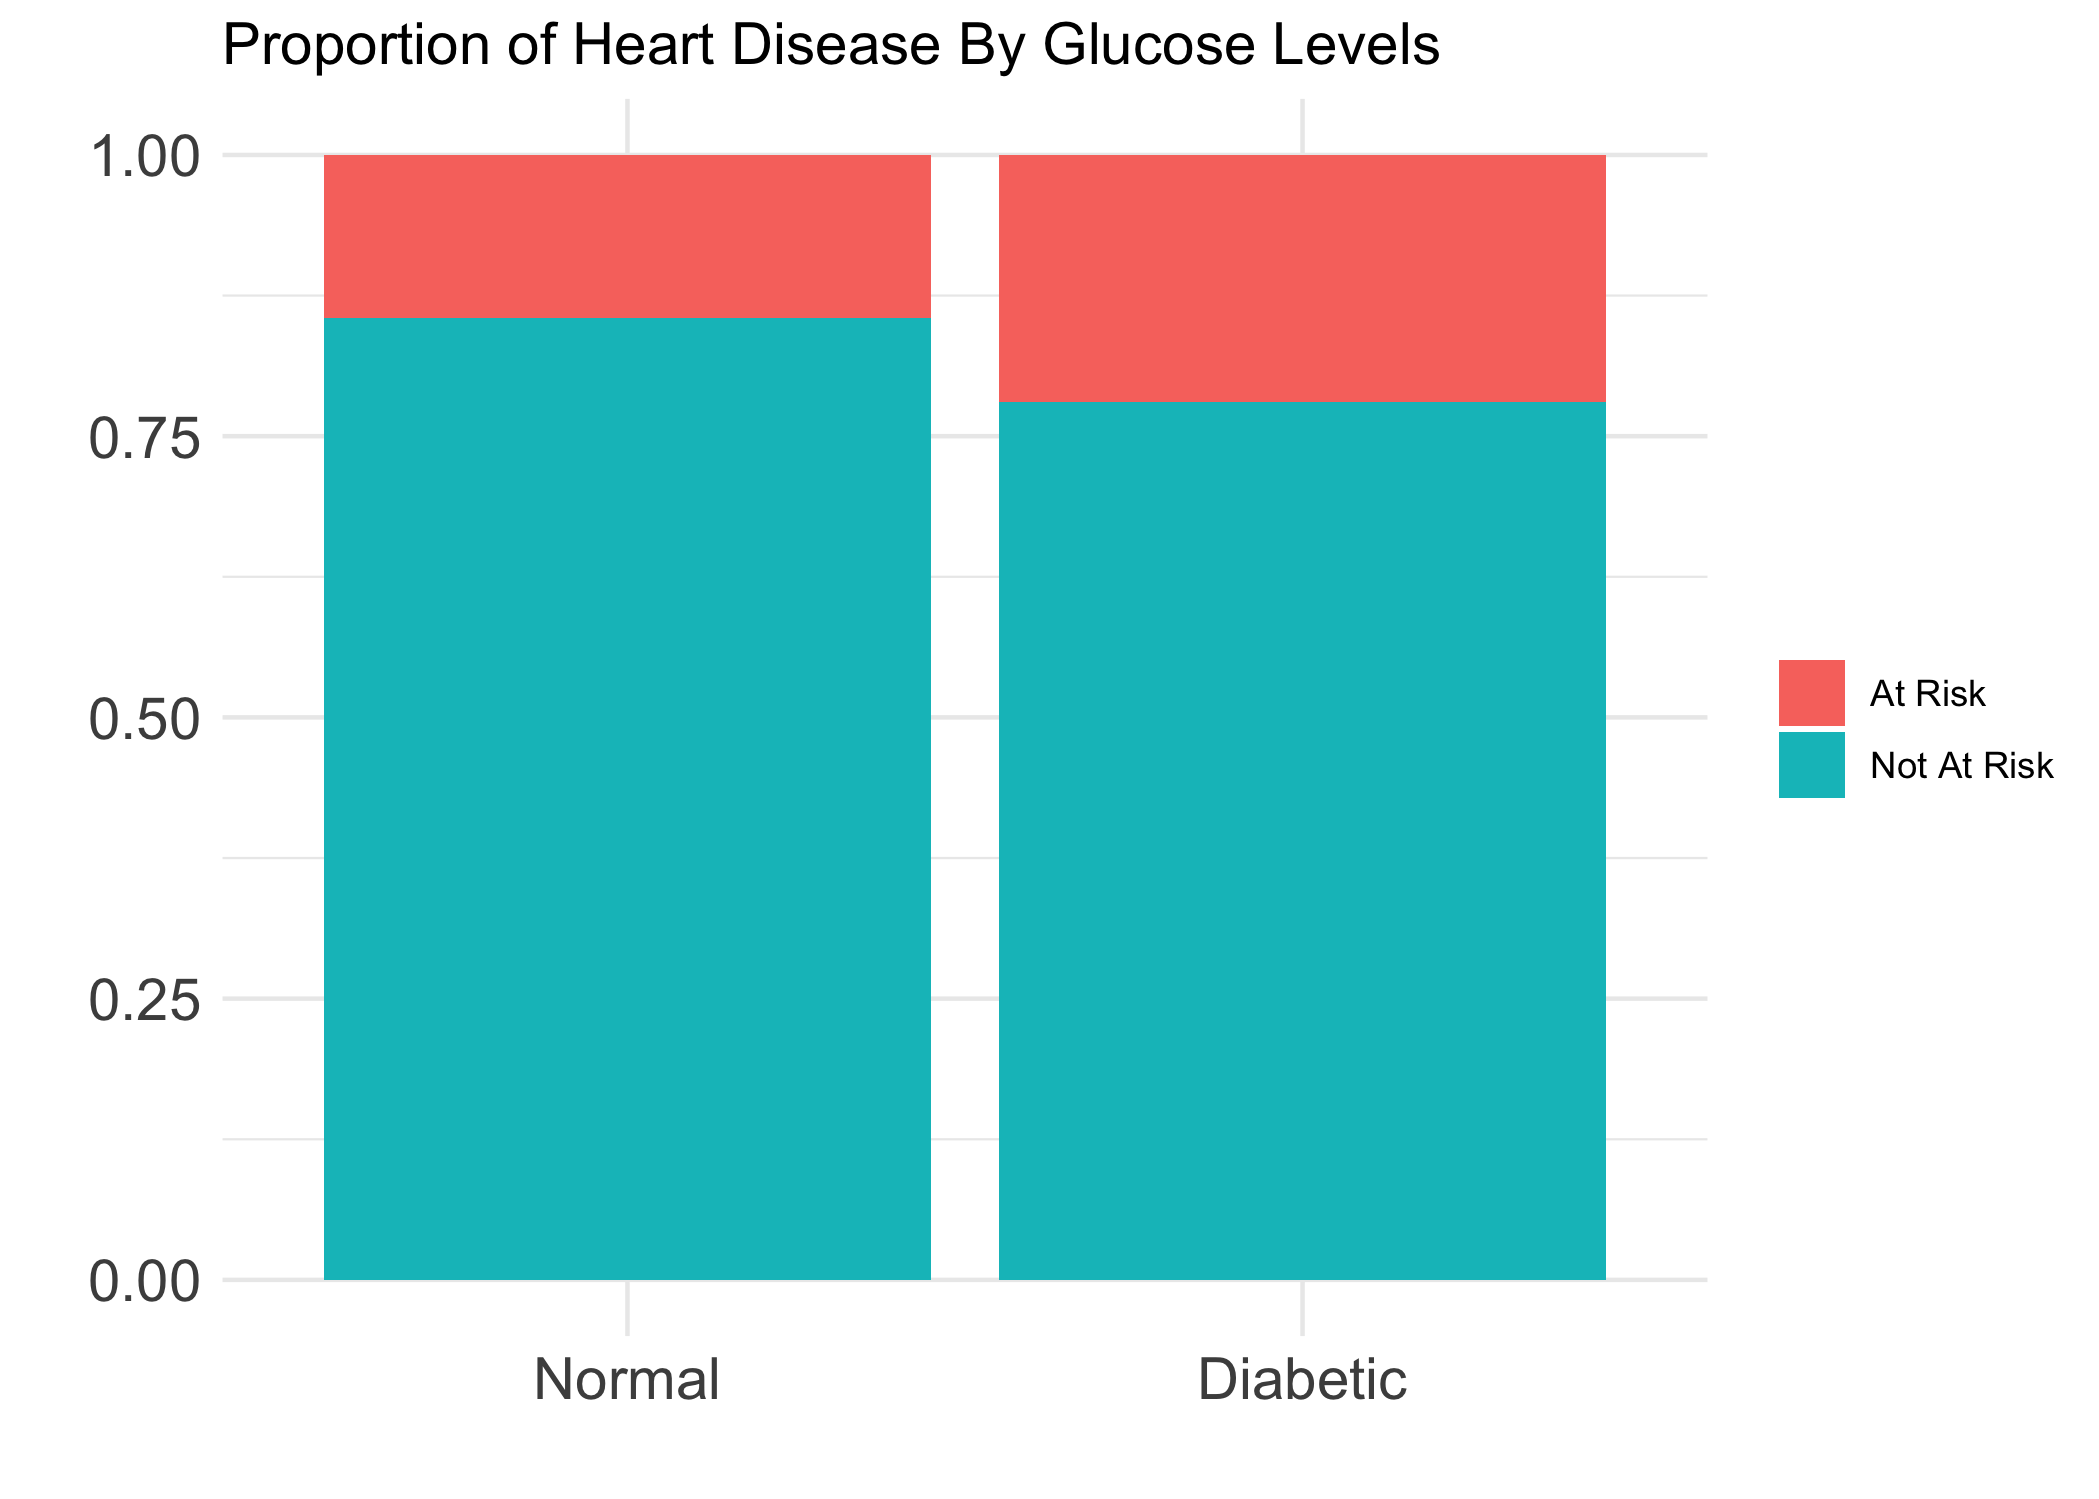
\includegraphics[height = 55mm, width=65mm]{two_way_glucose.png}}%
\hspace*{\fill}
\end{figure}


\subsubsection*{Multicollinearity}

To prepare for potential multicollinearity, we examined the correlation between the predictor variables and assessed the variance inflation factors (VIFs). Although diastolic and systolic blood pressure demonstrated strong correlation, the remaining pairs of variables did not display large correlations. As expected, we found that the two largest VIF scores belong to the systolic and diastolic blood pressure predictor variables. From the VIF plot below, we can see the predictors have VIF values less than four. Therefore, we did not investigate multicollinearity further. 

\begin{figure}[hbt!]
\hspace*{\fill}
\centering
\subcaptionbox{Variance Inflation Factor (VIF)}{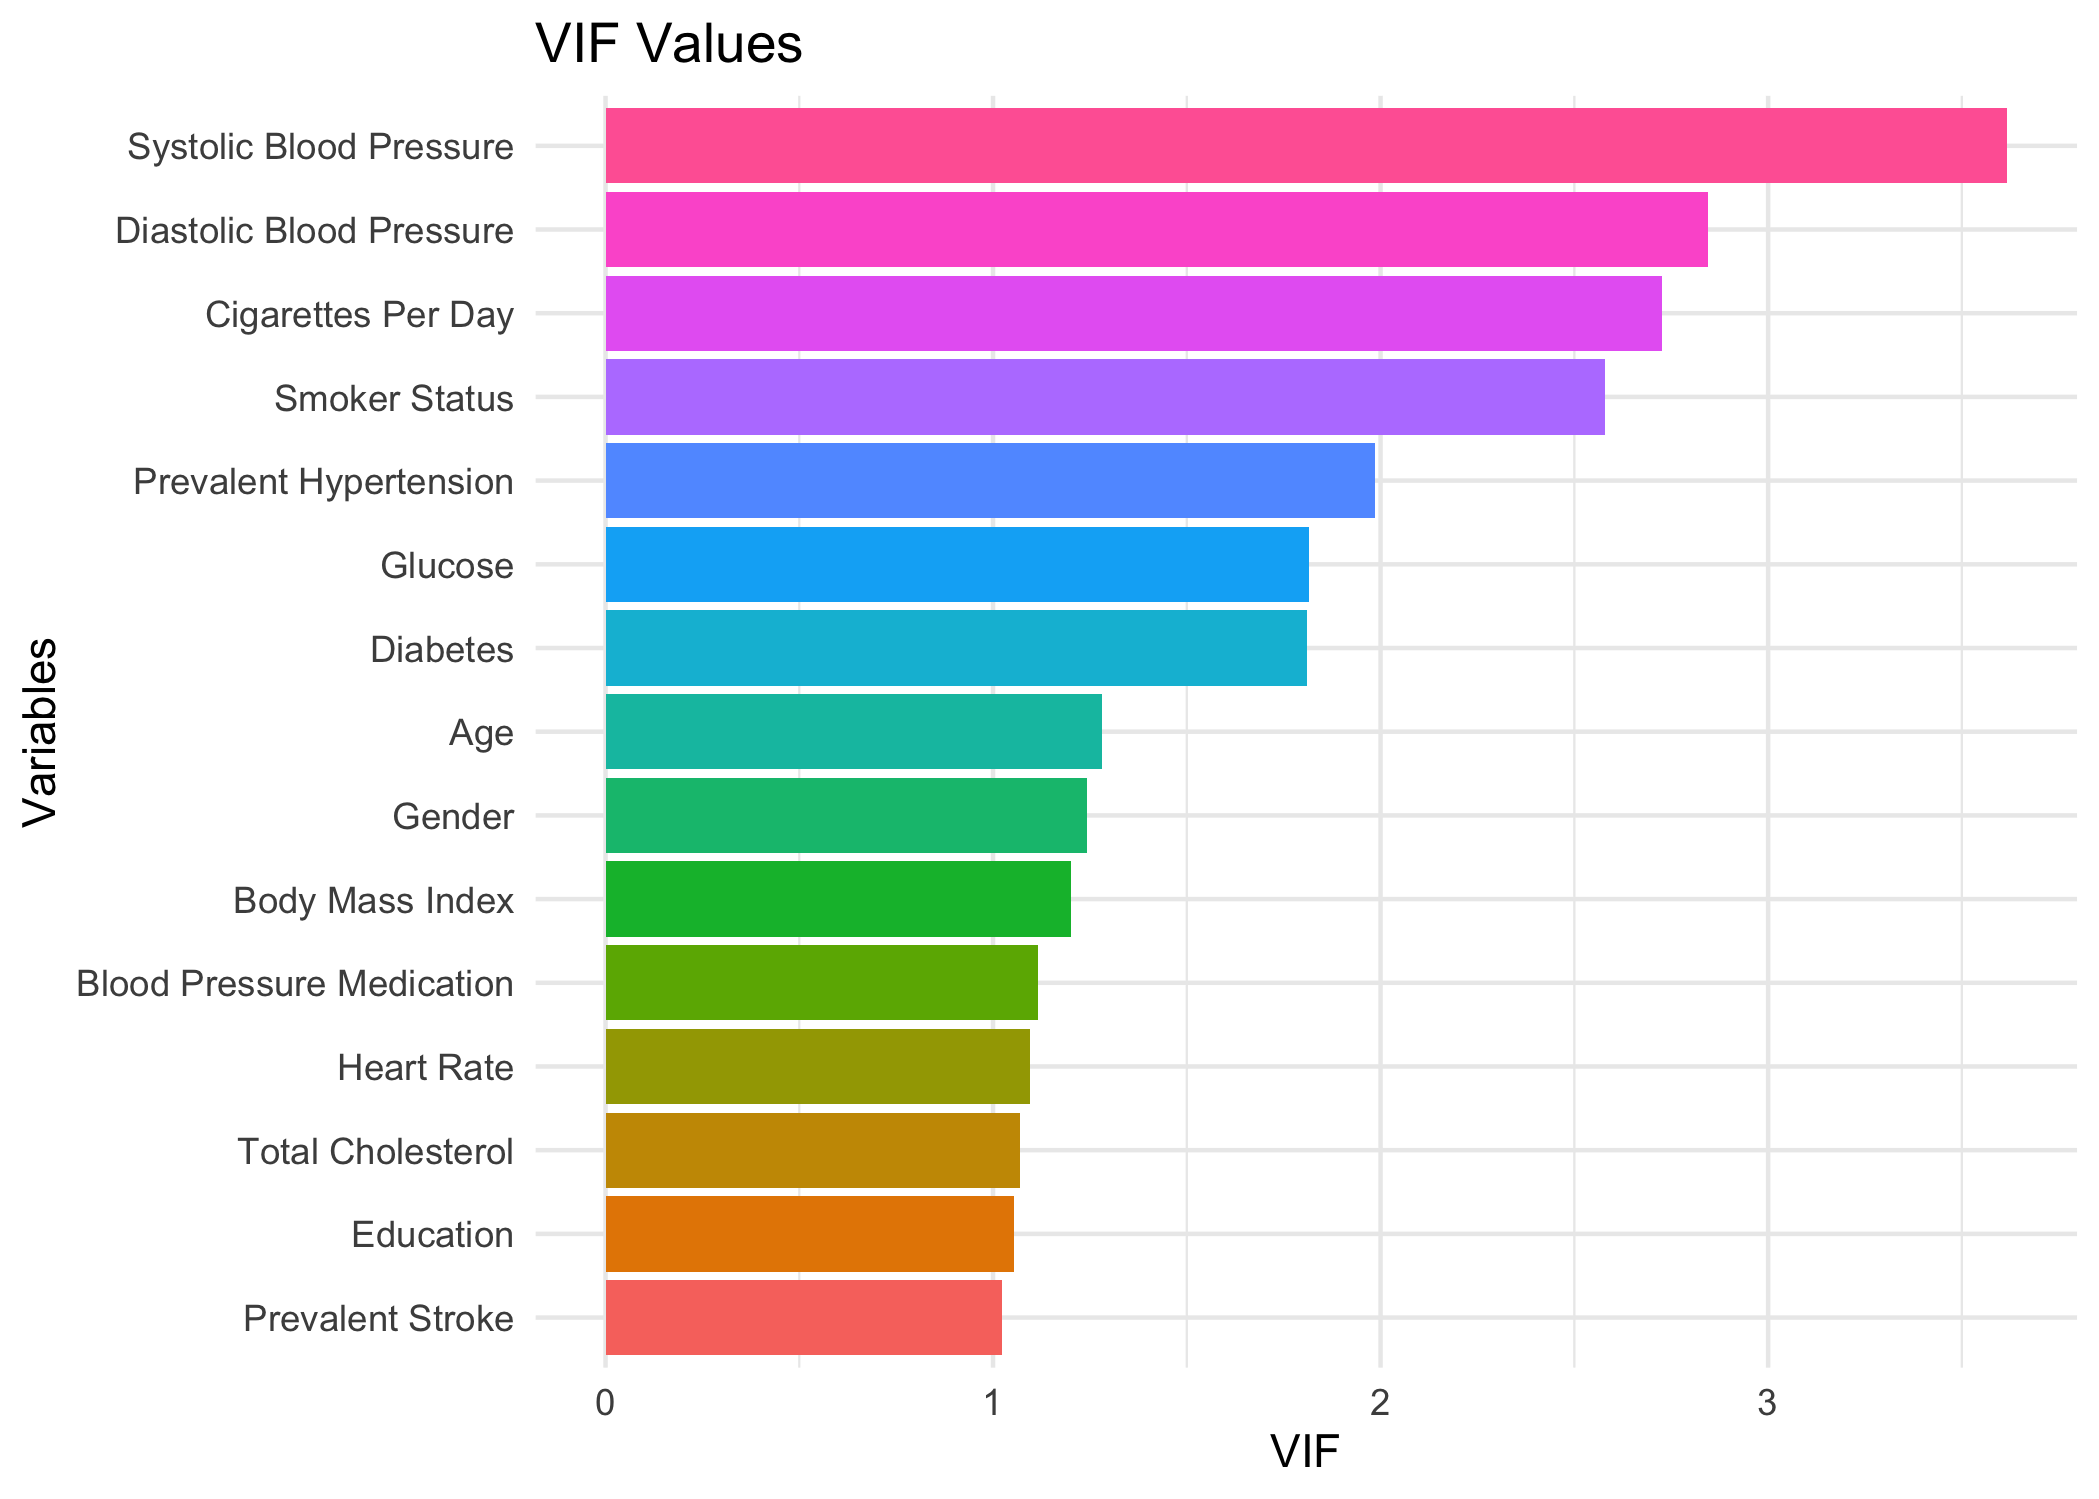
\includegraphics[height = 45mm, width=60mm]{vif.png}}\hspace{2em}
\subcaptionbox{Correlation Plot}{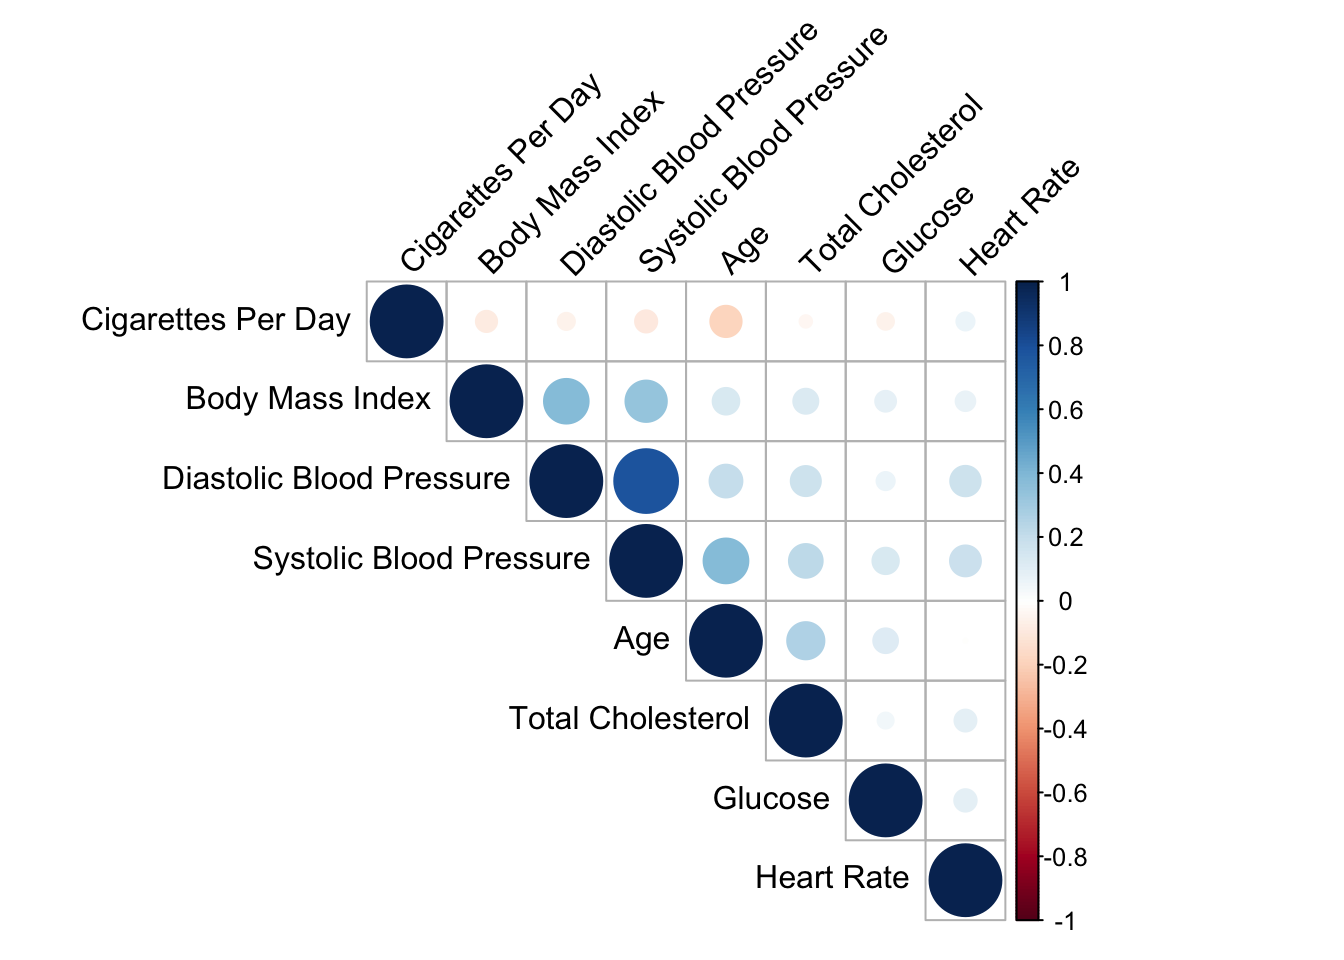
\includegraphics[height = 55mm, width=70mm]{corrplot.png}}%
\hspace*{\fill}
\end{figure}
 
During the modeling phase, the correlation between the two blood pressure variables may present multicollinearity. However, each model we used has its own form of variable selection that should help prevent the negative effects of highly correlated and unnecessary variables. We are confident multicollinearity will not be an issue later.


\section*{Feature Engineering}

After the exploratory data analysis with the original variables, we explored how interaction terms and quadratic terms could have a significant relationship with our response variable. 

\subsubsection*{Interaction Terms}

An interaction term is a new term that consists of two or more of the original variables. The table below shows a few of the significant numeric interaction terms.

\begin{table}[h!]
\centering
\begin{tabular}{| c | c | c | } 
\hline
Interaction & W & P-Value\\ 
\hline
\hline
Age w/ Cigarettes Per Day  &  935590  & 0.0007 \\
\hline
Systolic-BP w/ Cigarettes Per Day & 930899  & 0.0015 \\
\hline
Systolic-BP w/ Glucose  & 1102094  & 2.2e-16 \\
\hline  
\end{tabular}
\end{table}

\begin{figure}[hbt!]
\hspace*{\fill}
\centering
\subcaptionbox*{}{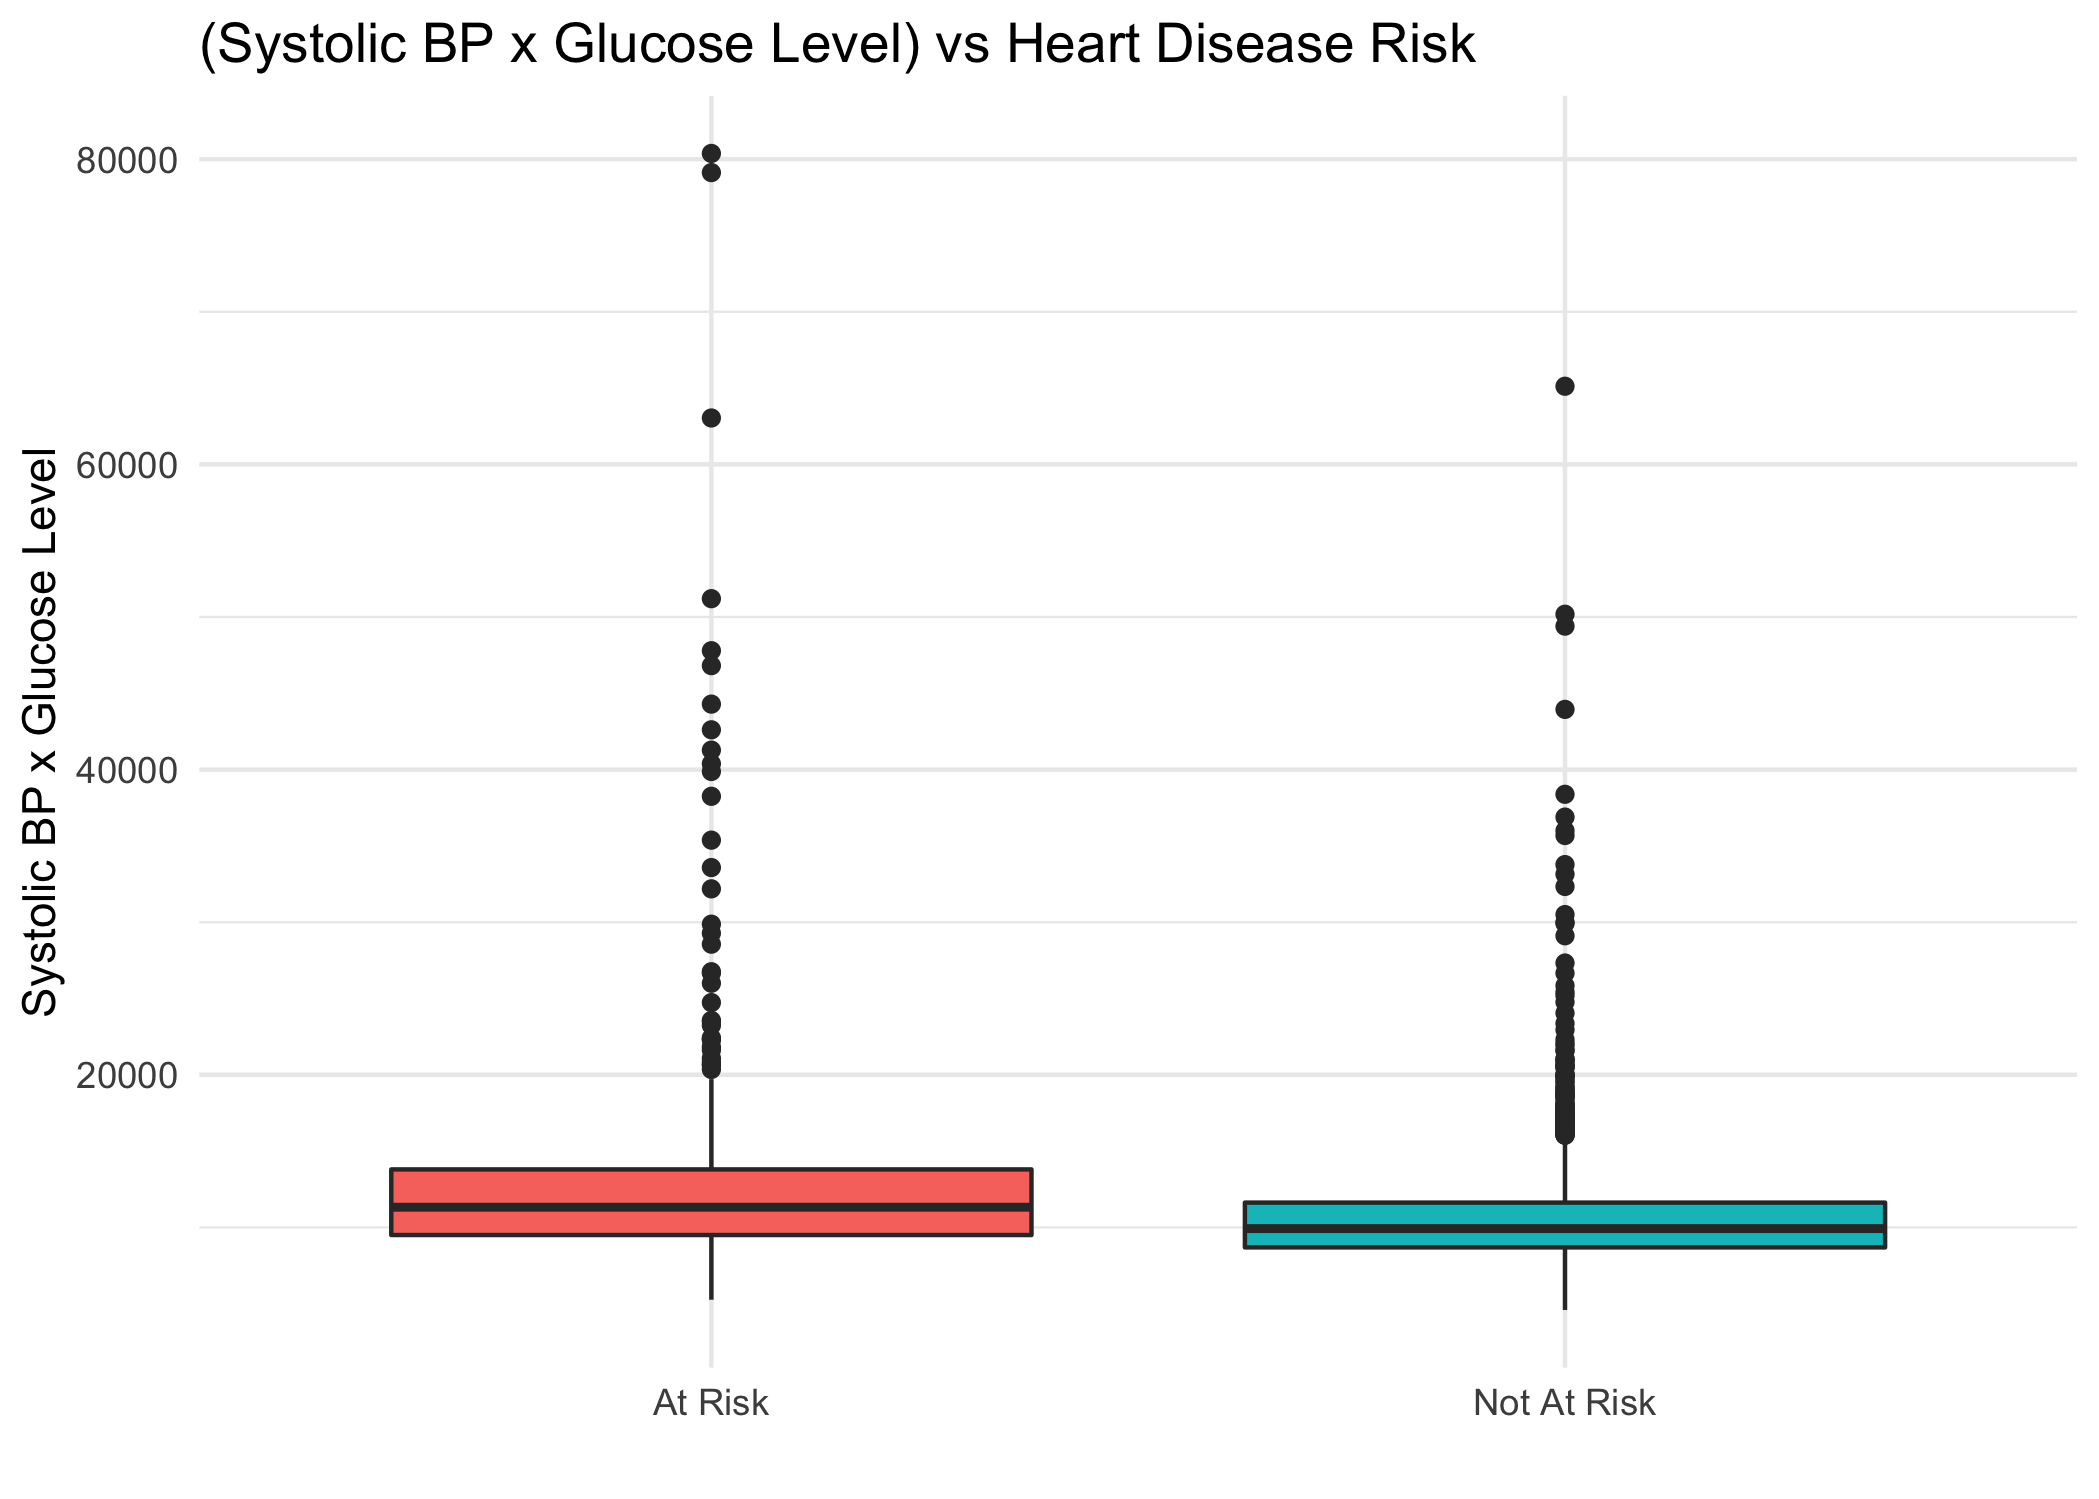
\includegraphics[height = 55mm, width=65mm]{box_int_sbp_glucose.png}}\hspace{2em}
\subcaptionbox*{}{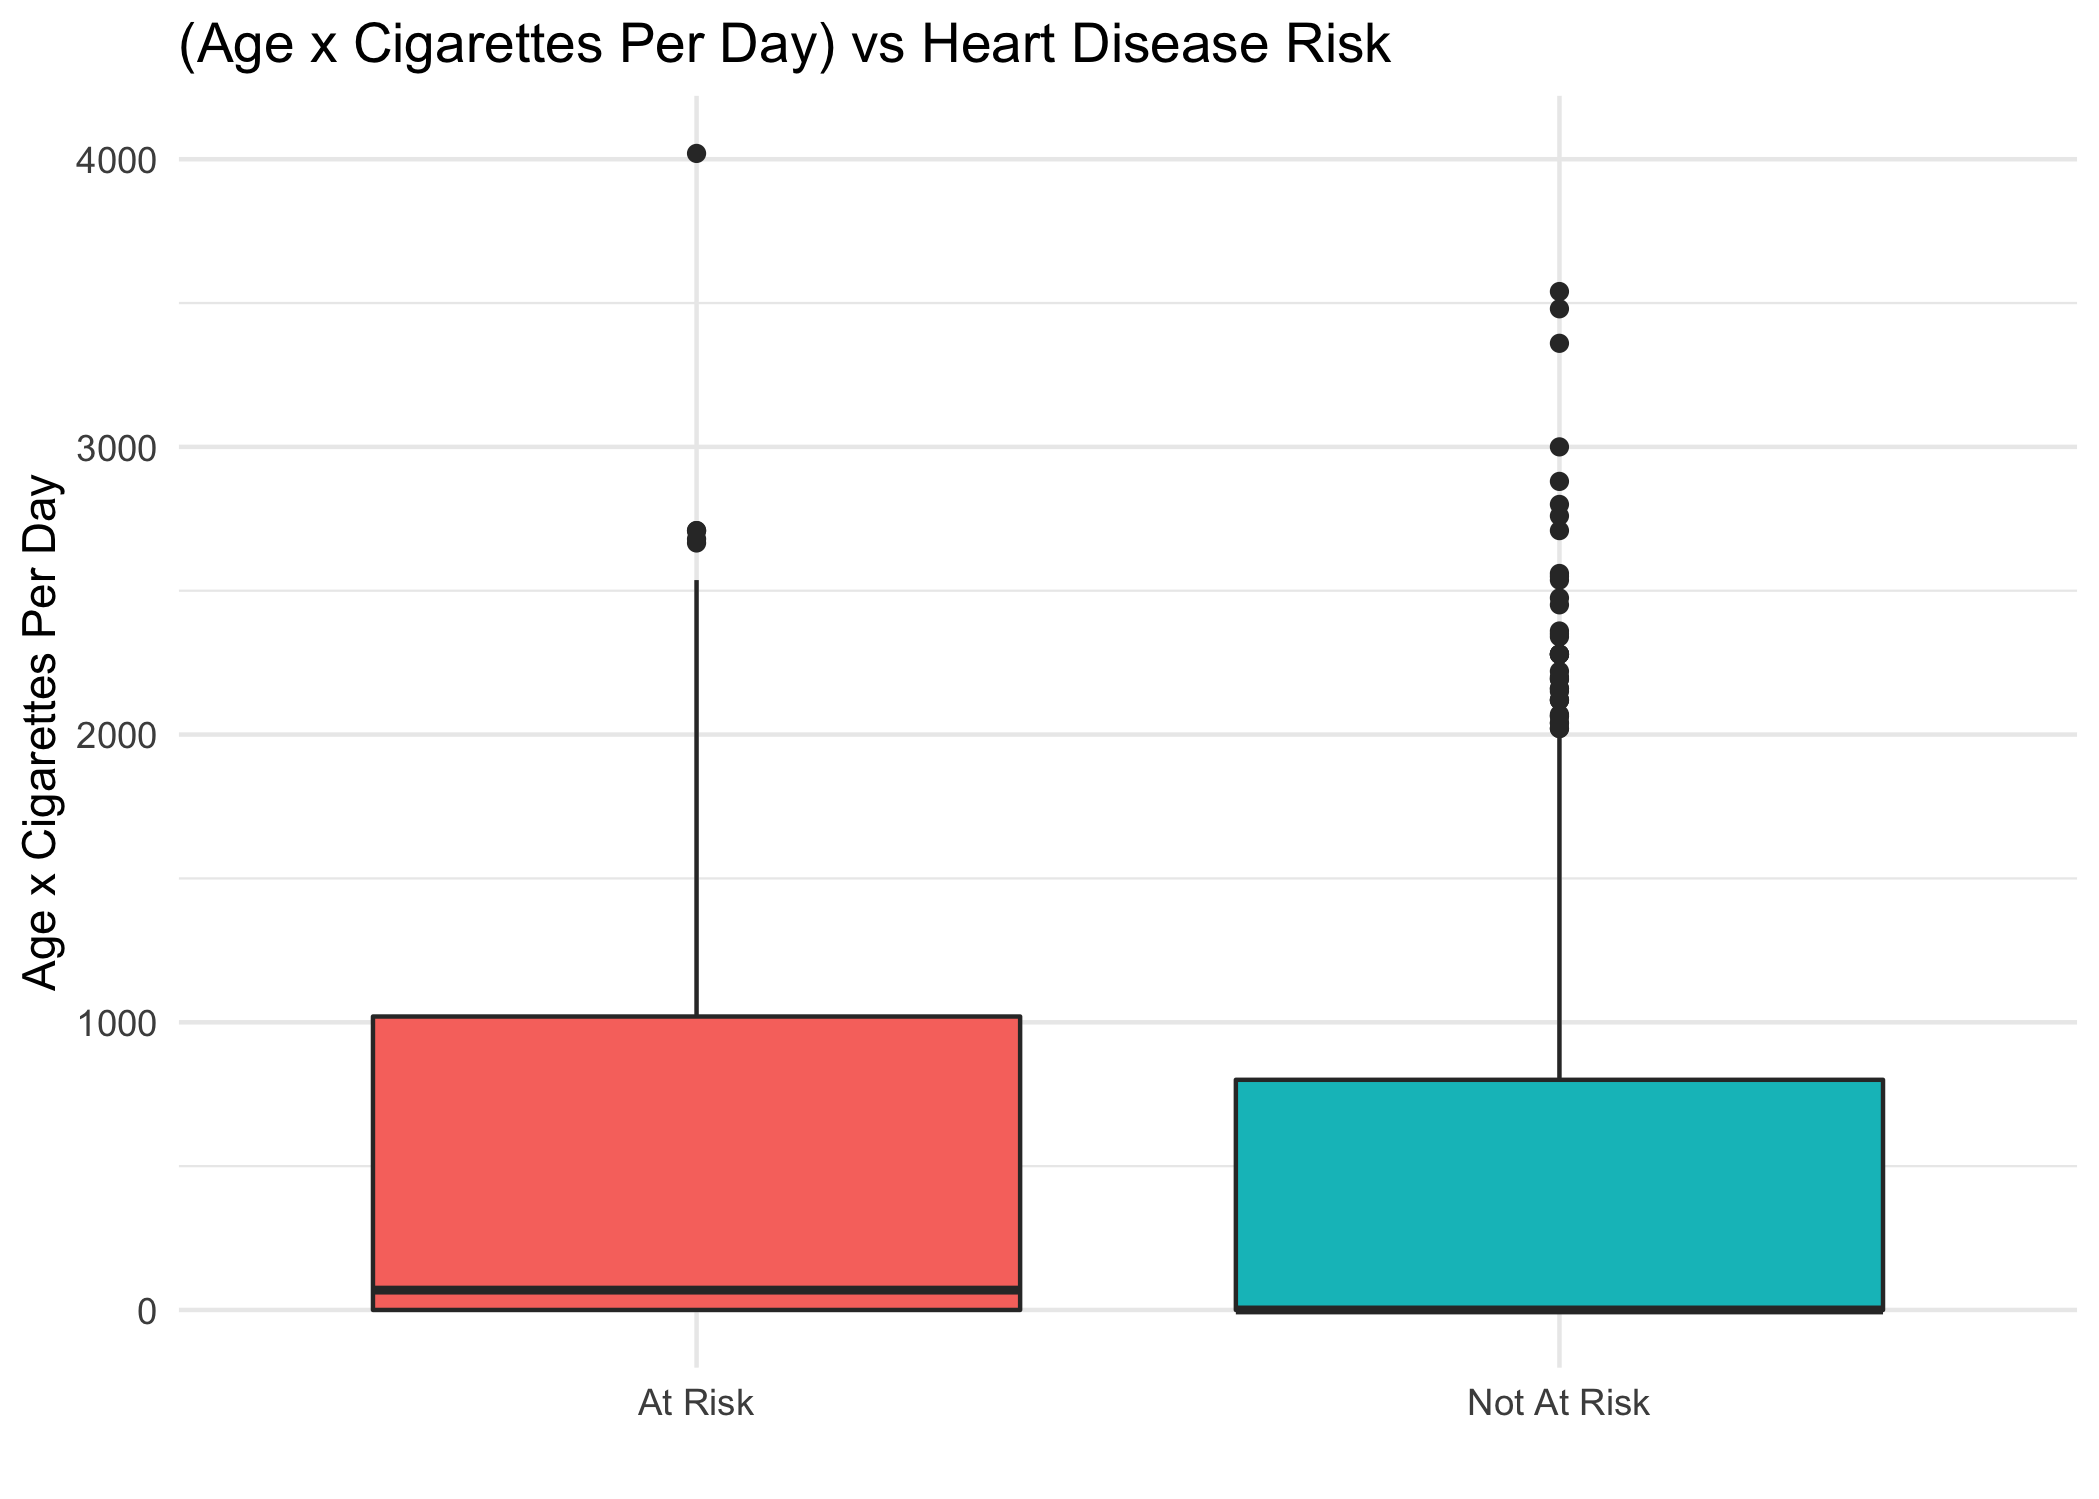
\includegraphics[height = 55mm, width=65mm]{box_int_age_cigs_per_day.png}}
\hspace*{\fill}
\end{figure}

Each interaction term has an underlying distribution. Depending on the underlying distribution, we either used a parametric or a non-parametric test to investigate if the interaction term has a significant effect on the response variable. Because the p-values above are small, we conclude that all three interaction terms are significant. The box-plots above provide further evidence that the interaction terms have an effect on the risk of heart disease.


\subsubsection*{Quadratic Terms}

Quadratic terms transform variables. In particular, quadratic terms square each value in a predictor variable and can be applied to every numeric variable in our data. However, it is unwise to do so. Squaring every variable in the dataset can lead to overfitting. Instead, we determined which numeric variables to square using a more mathematical approach.

\

Assuming that our response variable, $Y$, can be modeled with logistic regression, it can be shown that if a predictor variable, $X$, is normally distributed with different variances when conditioned on the two values of the response, then the log odds,

$$\log\frac{P(Y=1 | X = x)}{P(Y=0 | X = x)}$$

is a quadratic function of X such that, 

$$\log\frac{P(Y=1 | X = x)}{P(Y=0 | X = x)} = \beta_0 + \beta_1 x + \beta_2 x^2$$

for constants $\beta_0, \beta_1,$ and $\beta_2 \in \mathbb{R}$ (\cite{kay} \cite{cook}). 

\

Consequently, for each numeric variable, we compared the normalized conditional distributions similar to the plots shown below. If the conditional distributions appeared approximately normal but had significantly different sample variances, the variable became a candidate for a quadratic term.

\begin{figure}[hbt!]
\hspace*{\fill}
\centering
\subcaptionbox{}{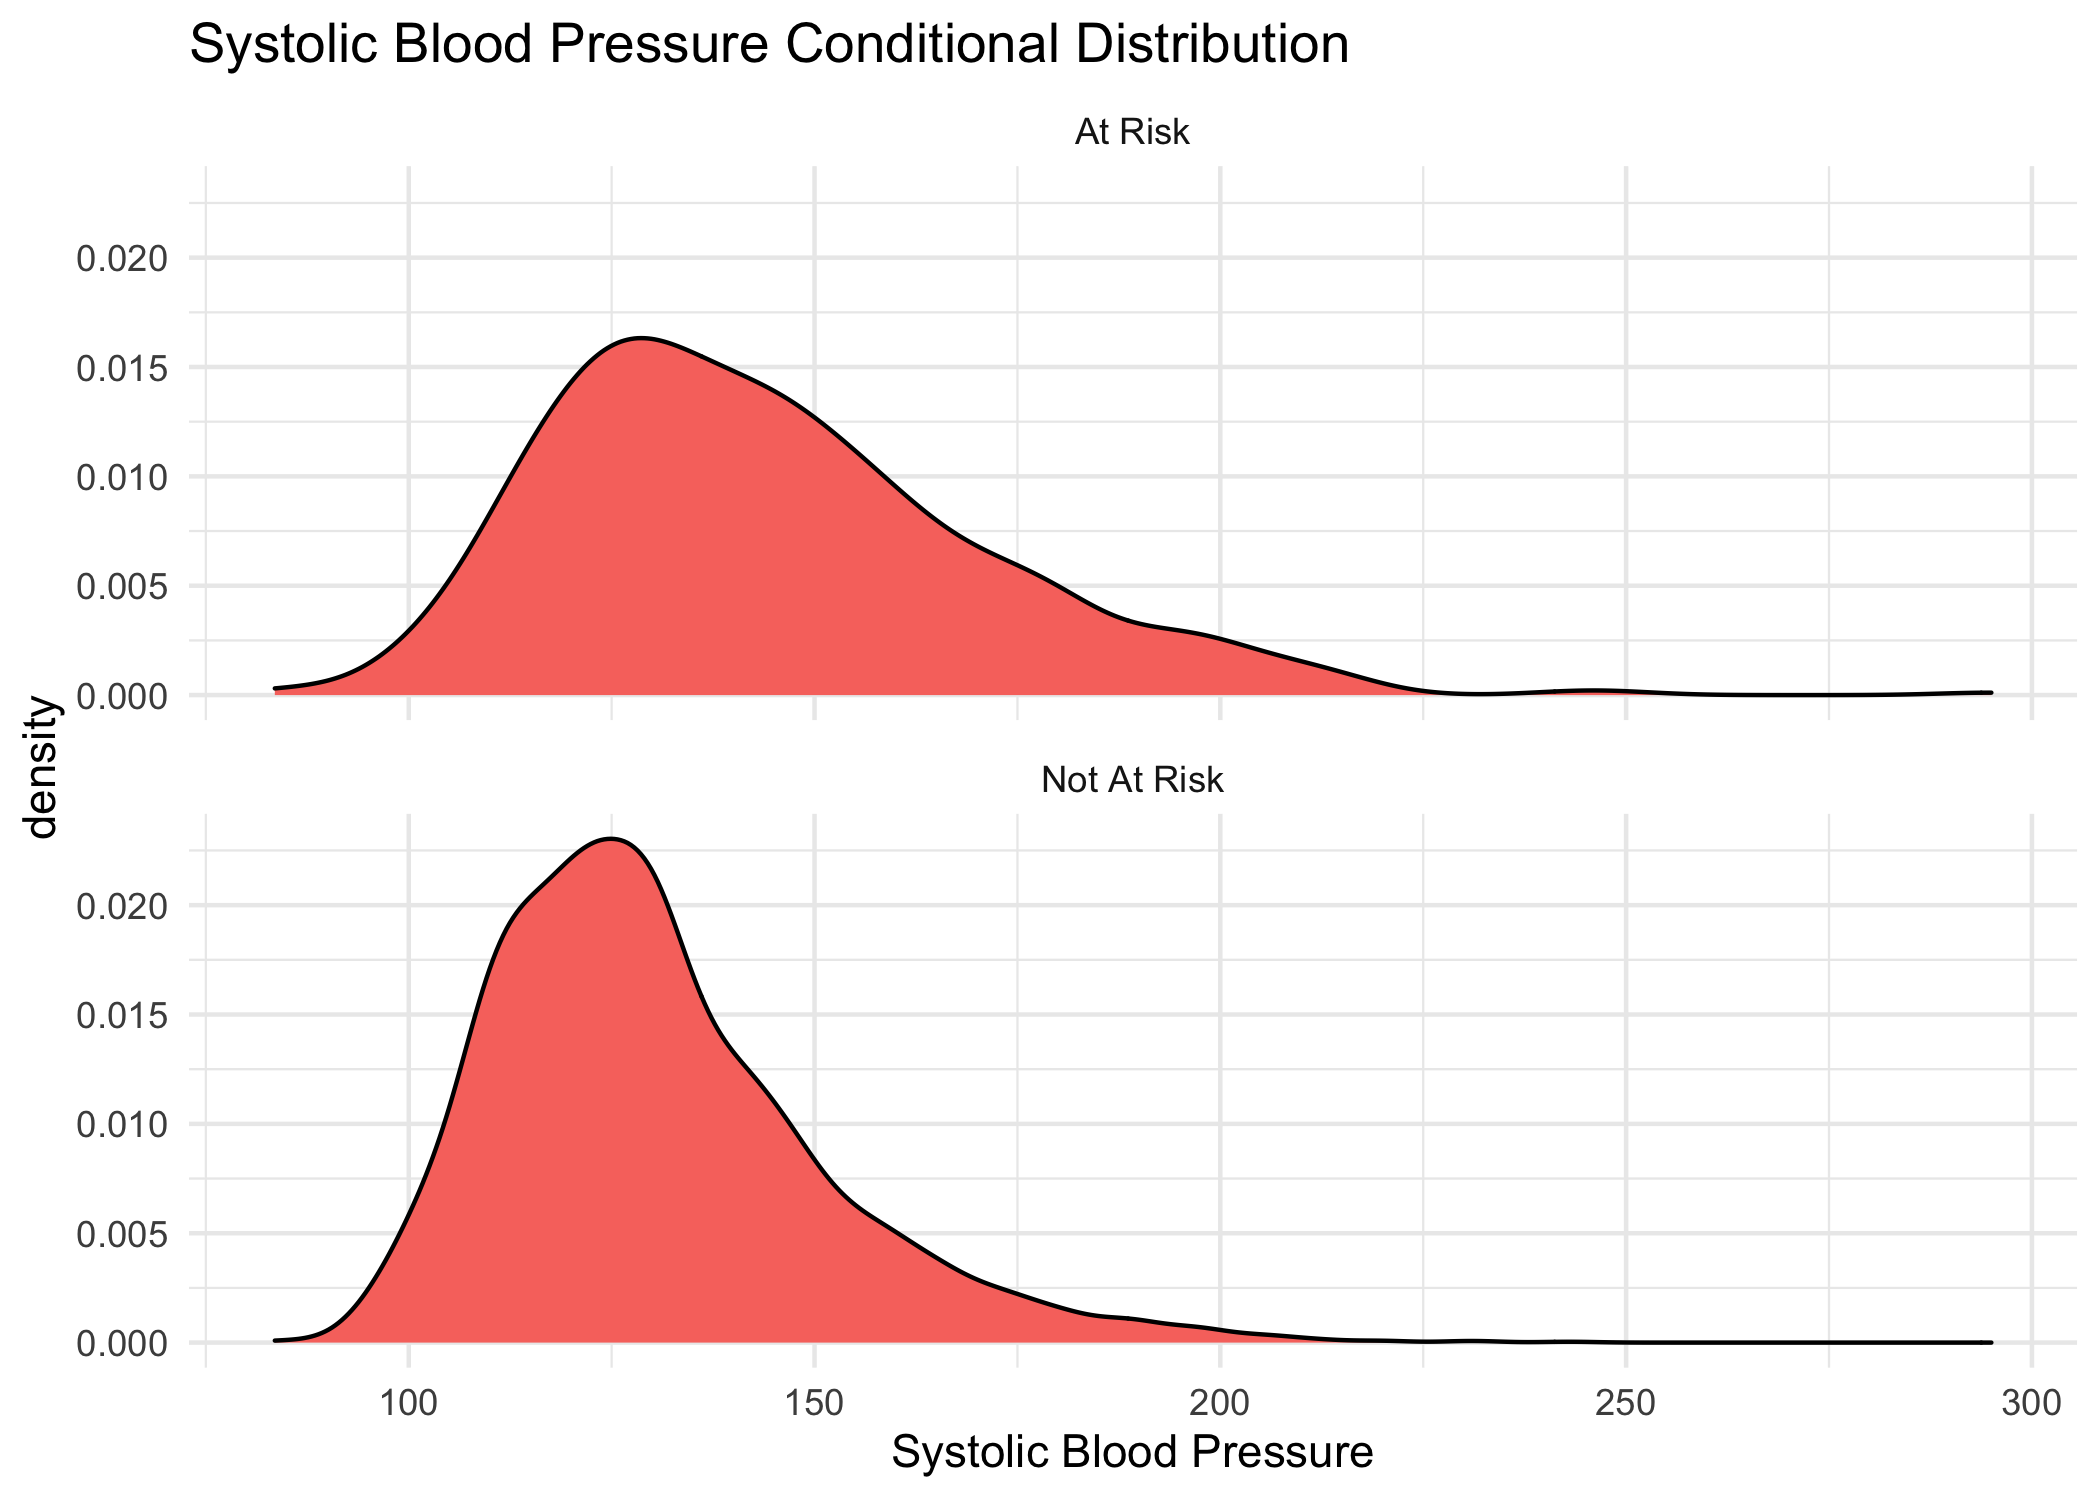
\includegraphics[height = 55mm, width=65mm]{dens_sbp.png}}\hspace{2em}
\subcaptionbox{}{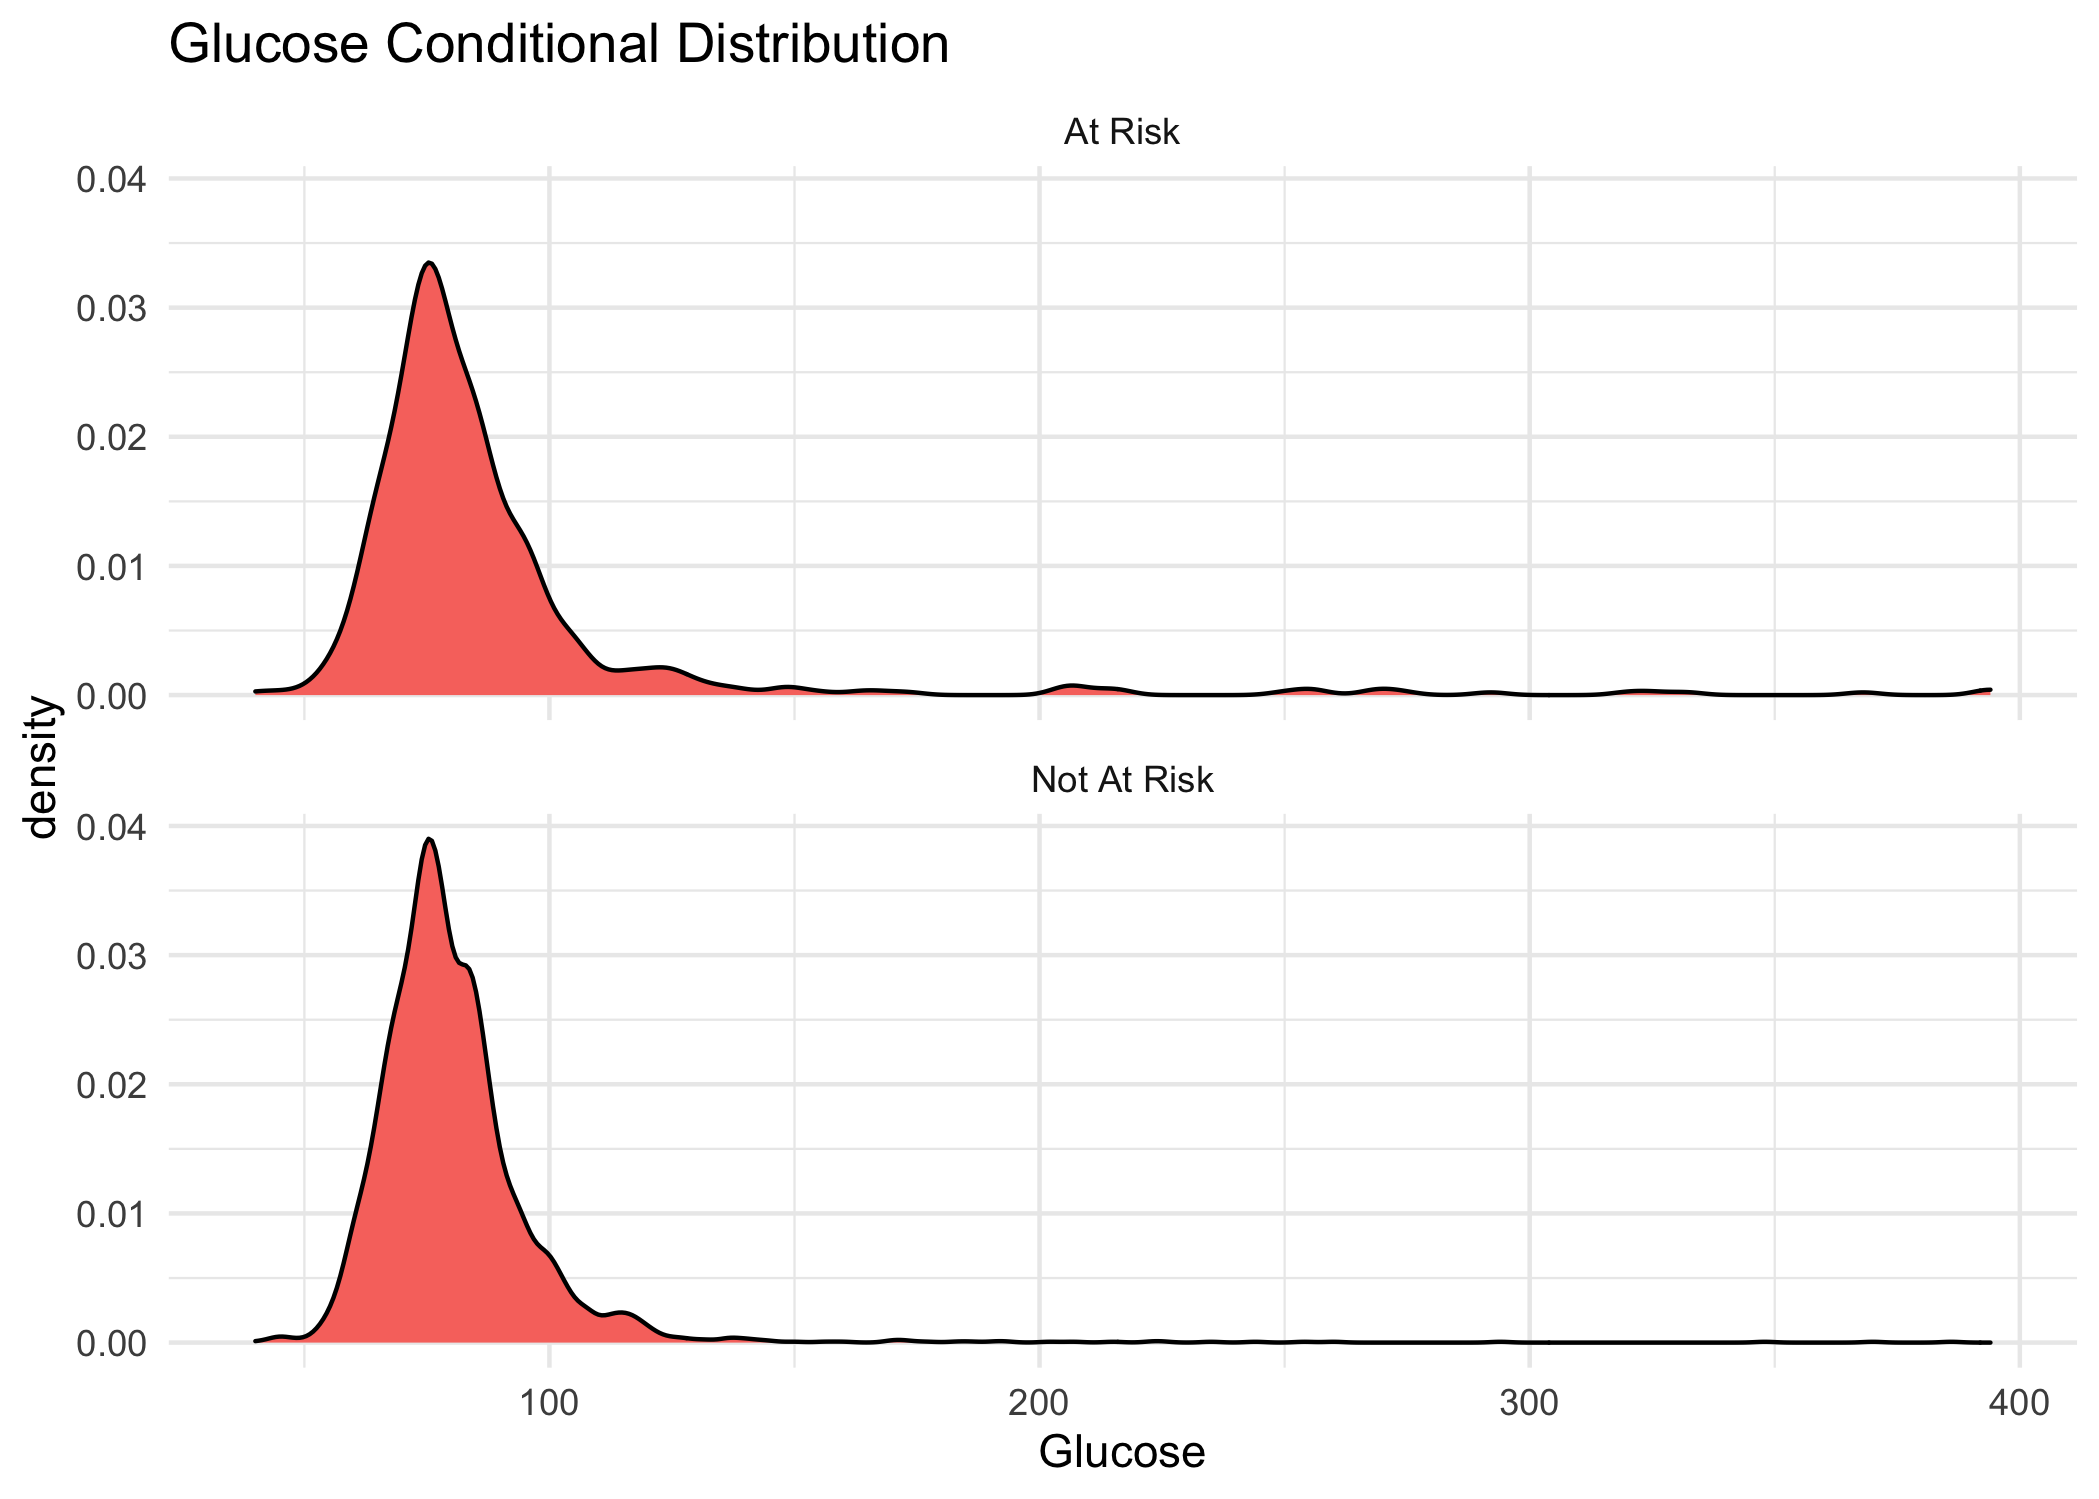
\includegraphics[height = 55mm, width=65mm]{dens_glucose.png}}
\hspace*{\fill}
\end{figure}

\begin{table}[h!]
\centering
\begin{tabular}{| c | c | c | } 
\hline
Predictor Variable & ``At Risk'' Std. Dev. & ``Not at Risk'' Std. Dev.\\ 
\hline
\hline
Systolic BP & 26.966 & 20.414 \\
\hline
Diastolic BP & 14.399 & 11.320 \\
\hline
Glucose & 40.786 & 19.129 \\
\hline  
\end{tabular}
\end{table}

The three predictor variables shown in the table above all approximately satisfied the requirements outlined before, so we chose to include their quadratic terms as new variables before we started the modeling. 


\section*{Methodology}

In this section, we describe the methods used to best predict the 10-year risk of future heart disease. First, our response variable is binary, so standard regression models will not work with our data. Instead, we used three different logistic regression models and one modern classification model to predict the probability of 10-year risk of future heart disease. 

\

Second, each model attempted to find the best combination of the predictor variables above. For all categorical variables, we created dummy variables with treatment coding (one-hot encoding). Note that the cigarettes-per-day and glucose variables above are actually continuous variables in the dataset. We portrayed them as categorical above to extract a more meaningful interpretation.

\

Third, we randomly split 80\% of the data into a training set and used the other random 20\% as the test set. The test set was not used by any model during the training process. Additionally, we partitioned 20\% of the training data into a validation set. Recall that our dataset is largely imbalanced. Approximately 85\% of the patients are not at risk of heart disease and approximately 15\% of the patients are at risk for heart disease. We ensured that each split of the data had a similar balance of patients that were not at risk and at risk of heart disease.

\

Since the response variable in the training data is imbalanced, we used randomized oversampling to combat any bias toward not having a risk of future heart disease. By oversampling, we hoped that the models would better detect when patients would be at risk for future heart disease. 

\

Lastly, we tuned each model's hyper-parameters. Using standard $k$-fold cross validation on the oversampled training data to tune our model's hyper-parameters would have led to overfitting and non-optimal hyper-parameters. Therefore, to ensure our models were not overfit to the oversampled training data, we used the independent validation set to tune each model's hyper-parameters. Once the hyper-parameters were obtained, we retrained the model on a new oversampled dataset made up of the original training set (without oversampling) and the validation set.

\

We evaluated and tuned each model with the area under the receiver operating characteristic (ROC-AUC) performance metric. We used the ROC-AUC over other metrics because it summarizes how well each model separates the two response classes for all possible thresholds (as opposed to a single predetermined threshold).

\subsubsection*{Logistic Regression with Backwards Elimination}

Our first model was a standard logistic regression model that started with all of the available predictor variables. This model used backwards elimination for feature selection. This process starts with all predictors in the model (full model), iteratively removes the least contributive predictors (using t-tests), and stops when the model's Akaike information criterion ($AIC$) can no longer decrease from a removal of an individual predictor variable. Ideally, this process will lead to a smaller, more significant, set of predictor variables and will be less likely to suffer from any overfitting or multicollinearity issues. After backwards selection, we refit the logistic regression model with the remaining significant variables. 

\subsubsection*{Logistic Regression with PCA}

Our next model uses a different approach for dimension reduction before fitting a logistic regression model. Principal component analysis (PCA) is often used to reduce the dimensions of a dataset by linearly transforming the data. A principal component is a linear combination of the predictor variables, and the entire set of principal components is mutually orthogonal. Each principal component attempts to explain as much of the variation in the feature space as possible, and all $n$ principal components account for 100\% of the variation in the data. Similar to backward selection, the goal here is to use $k < p$ principal components to mitigate any effects of multicollinearity and to prevent the chance of overfitting.

\

Recall that many of our predictors are in different units, so we chose to center and scale our data to prevent variables with larger values from dominating the sample variance explained. After we calculated all $p$ principal components, we used a combination of scree plots and validation data to evaluate the variance explained and predictive performance of the first $k$ principal components where $k$ ranges from 1 to $p$. Once we obtained the optimal number of principal components, $\hat{k}_{best}$, we refit the logistic regression model with the first $\hat{k}_{best}$ principal components from the entire training set.

\subsubsection*{Logistic Regression with Elastic Net Regularization}

Our last logistic regression model uses another form of variable selection known as \textit{regularization}. In general, regularization adds a penalty for each additional predictor variable in the model, and minimizes overfitting by removing or shrinking the effect of unnecessary predictor variables. Elastic net regularization combines two common regularization techniques, LASSO and Ridge (also known as $L1$ and $L2$ penalties), with the following formula:

$$\hat{\boldsymbol{\beta}} = \argmin_{\boldsymbol{\beta}} \left( -\frac{1}{n} \sum_{i = 1}^{n} l(x_i, y_i; \boldsymbol{\beta}) + \lambda \left[(1- \alpha)\frac{||\boldsymbol{\beta}||_{2}^{2}}{2} + \alpha||\boldsymbol{\beta}||_{1} \right] \right)$$

where $l(x_i, y_i; \boldsymbol{\beta})$ is the log-likelihood contribution for the $i$th observation. To ensure a fair penalization of each predictor variable, we centered and scaled the data before training the elastic net model. Using results from our dedicated validation set, we tuned this model to find the optimal values for the mixing parameter, $\alpha$, and the regularization parameter, $\lambda$. We then refit the logistic regression model to the entire training set with the optimal hyper-parameters, $\hat{\alpha}$
and $\hat{\lambda}$.

\subsubsection*{eXtreme Gradient Boosting (XGBoost)}

Lastly, we fit an extreme gradient boosting classification model to predict the 10-year risk of heart disease. XGBoost is a decision-tree based algorithm that uses penalized trees, proportional leaf node shrinking, and automatic variable selection, among other features. In general, this model minimizes its respective loss function by adding the individual contributions from an ensemble of weak learners. Additionally, XGBoost is trained using a second order gradient optimization algorithm. For simplicity, we used the validation set to tune the number of trees (weak learners) used and the maximum depth of each tree.

\subsubsection*{Model Evaluation and Comparison}

To examine and compare each model's predictive performance, we use our (completely unseen) test data. For each model, we generated predicted probabilities for the test set to obtain visuals such as ROC Curves, accuracy plots, sensitivity plots, specificity plots, and false positive plots. In addition to the visuals, we also computed quantitative measures such as the area under the ROC curves, confusion matrices, and a variety of other performance metrics. 

\

Although visuals and metrics such as the ROC curve and ROC-AUC consider \textit{all} thresholds, most of the other measures mentioned above require a specified probability threshold to generate class predictions. Given that our models are attempting to predict the presence of a life-threatening condition, we wanted to find a threshold that prioritizes true positives while not overly accepting too many false positives. In addition, we prefered to optimize our threshold in a way that does not unfairly suffer from the large class imbalance in our data. Therefore, we used the geometric mean of the \textit{sensitivity} (or true positive rate) and the \textit{specificity} (or true negative rate), 

$$G_{mean}(t) = \sqrt{\text{Sensitivity} \cdot \text{Specificity}} = \sqrt{\frac{TP \cdot TN }{(TP + FN)(TN + FP)}}$$

to determine an optimal threshold for each model. That is, for each model, we found the threshold $t^* \in (0, 1)$ that maximizes the geometric mean, $G_{mean}(t)$. Note that only the training and validation sets were used to find $t^*$ so that we can retain a completely unseen testing set when evaluating and comparing model performances. 

\section*{Results and Discussion}

\subsubsection*{Logistic Regression with Backwards Elimination}

Using backwards elimination, the logistic regression model went from the original set of 23 predictors to 13 predictors. Most of the remaining predictor variables were statistically significant at the $\alpha = 0.05$ level. The backwards elimination dropped the $AIC$ score from 2851.2 with the full model to 2836.6 with the reduced model, indicating potential improvement in the model. We tested the hypothesis that the reduced model is adequate by comparing the residual deviance of the reduced model to the residual deviance of the full model using all of the predictors. The table below shows the results of this test. We can see from the large p-value that we did not have enough evidence to reject the null hypothesis, and concluded that the model using the reduced number of predictors is adequate.

\begin{table}[h!]
\centering
\begin{tabular}{| c | c | c | c | } 
\hline
& Resid. Df & Resid. Dev & Pr($>$Chi) \\ 
\hline
\hline
Reduced Model & 2327 & 2808.6 & \\
\hline
Full Model & 2317 & 2803.2 & $\approx 0.864$\\
\hline  
\end{tabular}
\end{table}

Again using residual deviance, we also tested our model against the null model (with $H_0: \beta_i = 0$ for all $i$). As indicated by the table below, we rejected the hypothesis and concluded that our model demonstrated strong significance between the predictors and the response. 

\begin{table}[h!]
\centering
\begin{tabular}{| c | c | c | c | } 
\hline
& Resid. Df & Resid. Dev & Pr($>$Chi) \\ 
\hline
\hline
Null Model & 2340 & 3245.3 & \\
\hline
Model Using Predictors & 2327 & 2808.6 & $\approx 0$\\
\hline  
\end{tabular}
\end{table}

To assess our model's fit, we visually examined the Pearson Residuals vs Predicted Values plot and used the Pearson's $\chi^2$ goodness-of-fit test to test the hypothesis that our model fit the data sufficiently well. The Pearson's $\chi^2$ goodness-of-fit test had a p-value of 0.22, which indicated that our model fit the data sufficiently well. 


\begin{figure}[hbt!]
\hspace*{\fill}
\centering
\subcaptionbox*{}{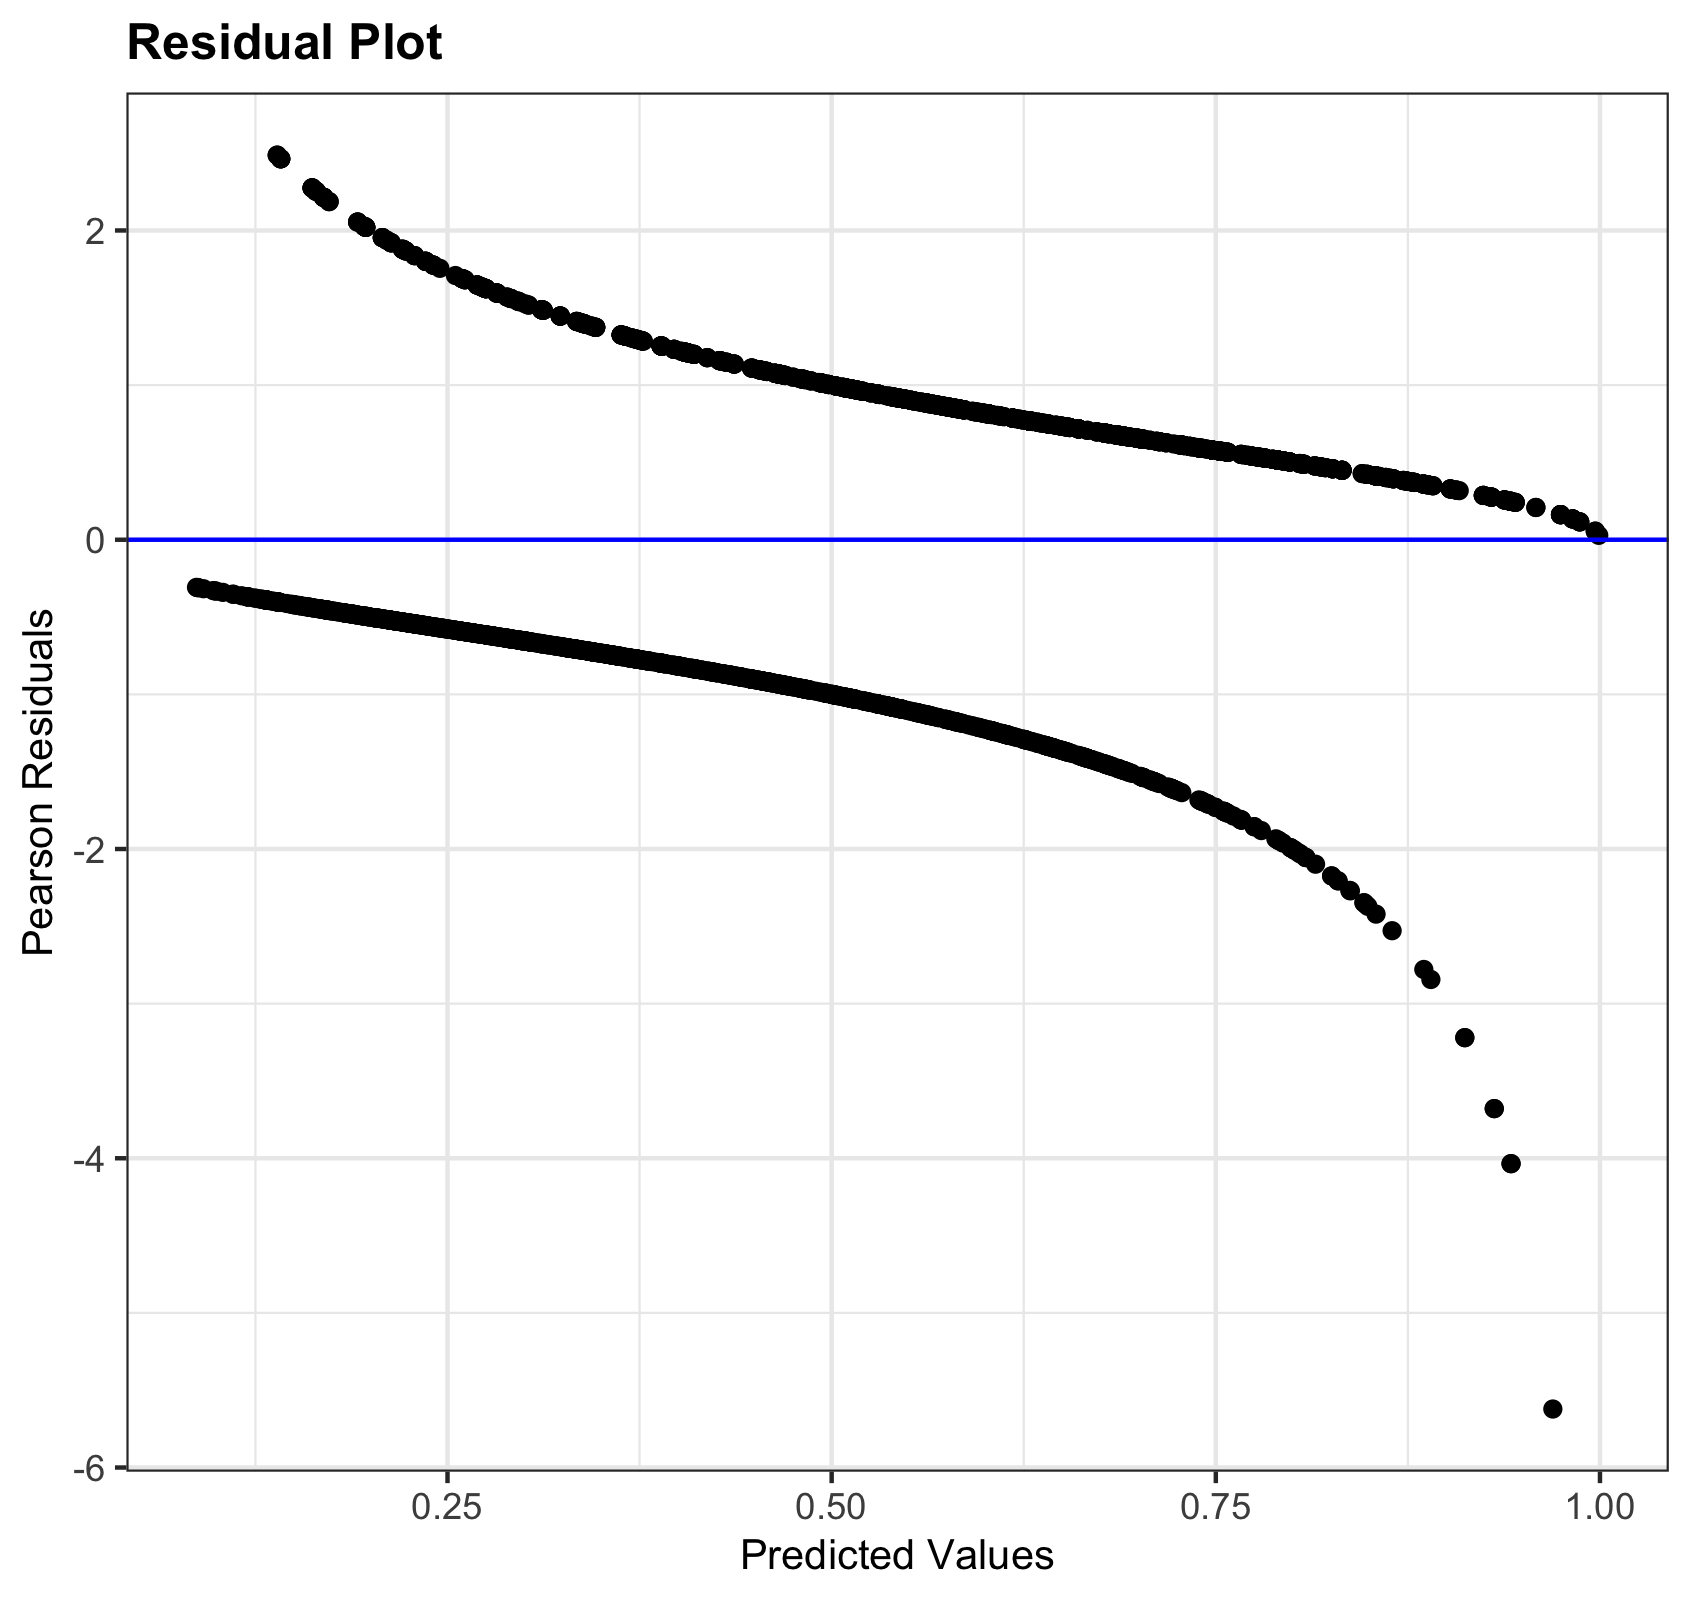
\includegraphics[height = 60mm, width=70mm]{subset_LR_pearson_residuals_ONLY.png}}\hspace{2em}
\subcaptionbox*{}{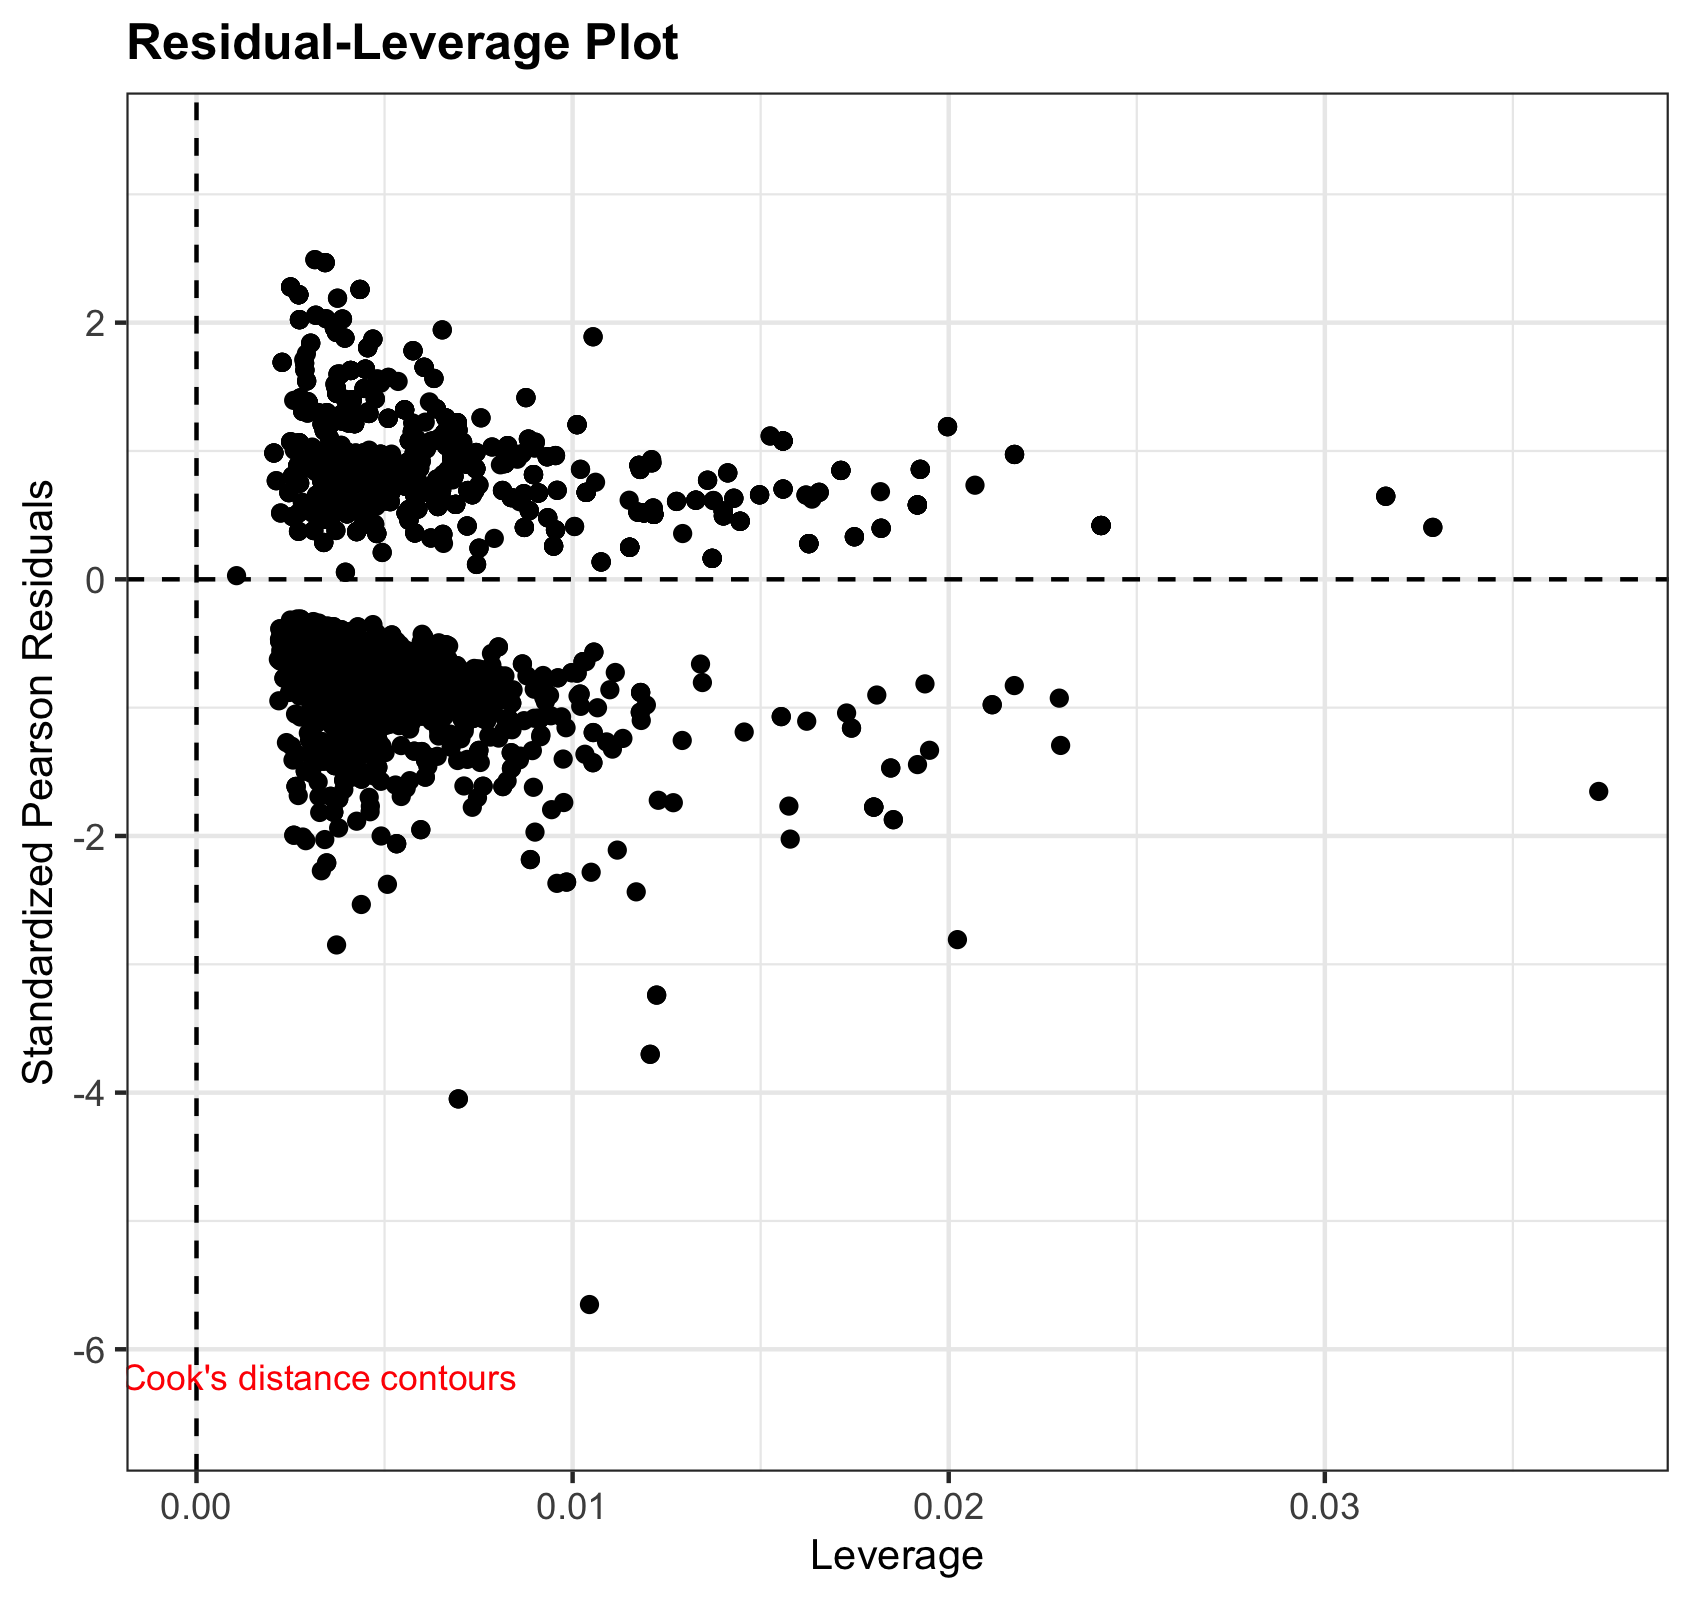
\includegraphics[height = 60mm, width=70mm]{subset_LR_pearson_lev_ONLY.png}}
\hspace*{\fill}
\end{figure}

Plots of Std. Pearson Residuals vs Leverage and Cook's distances were also assessed to check for potentially dangerous influential points. No observations demonstrated an unusually large combination of leverage and residual magnitude. Therefore, no observations were removed from the training set.

\
 
The remaining coefficients $\beta_1, \beta_2, ..., \beta_{13}$ for this logistic regression model are presented in the table below. Since we centered and scaled our data before fitting the logistic regression model, each coefficient from the table below can be interpreted very easily. Recall that for continuous variables, each coefficient effectively represents the increase in the log odds for every standard deviation increased in the predictor variable, holding all else constant. Additionally, for categorical variables, each coefficient simply represents the increase in log odds when the variable is associated with the corresponding category as opposed to the reference category, holding all else constant. This is also known as the \textit{log-odds ratio}.

\

We can exponentiate the coefficients to obtain an equivalent interpretation in terms of the odds. For example, we can see from the table below that one standard deviation increase in age is associated with a 6\% ($e^{\hat{\beta}_{2}} = 1.06$) increase in the odds of a patient having a 10 year risk of heart disease. As another example, we can see below that a patient with hypertension is associated with a 15\% ($e^{\hat{\beta}_{8}} = 1.15$) increase in the odds of having a 10 year risk of heart disease.

\begin{table}[h!]
\centering
\begin{tabular}{| c | c | c | c | } 
\hline
&  &  &  \\ 
Predictor & Estimate ($\hat{\beta}_i$) & $e^{\hat{\beta}_i}$ & P-Value (Wald) \\
&  &  &  \\ 
\hline
\hline
Gender (male) & 0.592 & 1.80 & $\approx 2.71e-11$\\
\hline
Age & 0.064 & 1.06 & $< 2e-16$\\
\hline  
Education (High School) &  -0.093  & 0.911  & $\approx 0.362$\\
\hline    
Education (Bachelors) &  -0.452 & 0.641 &  $\approx 0$\\
\hline
Eucation (Graduate) & -0.186 &  0.830 & $\approx 0.161$\\ 
\hline
Cigarettes per Day &  0.024 &  1.02 & $\approx 2.16e-11$\\ 
\hline
BP Medication  & 0.801 &  2.228 & $\approx 0.003$\\
\hline
Prevalent Hypertension & 0.141 & 1.151 & $\approx 0.242$\\  
\hline 
Total Cholesterol & 0.004 & 1.004 & $\approx 0$\\
\hline
Systolic BP & 0.011 & 1.011 & $\approx 0.001$\\
\hline
Diastolic BP & -0.118 &  0.888 & $\approx 0$\\
\hline
Diastolic BP (Squared) & 0.001 & 1.001 & $\approx 0$\\
\hline 
Glucose (Squared) & 0.000 & 1.00 & $\approx 0$\\
\hline 
\end{tabular}
\end{table}


\subsubsection*{Logistic Regression with PCA}

After performing PCA on our training set, we found that the first 9 sample principal components explained over 80\% of the sample variance of our data, and the first 12 principal components explained over 90\% of the sample variance. The plot (left) below shows the sample variance explained from each sample principal component computed (23 in total). There is a clear “elbow” in the plot at the 4th sample principal component.


\begin{figure}[hbt!]
\hspace*{\fill}
\centering
\subcaptionbox*{}{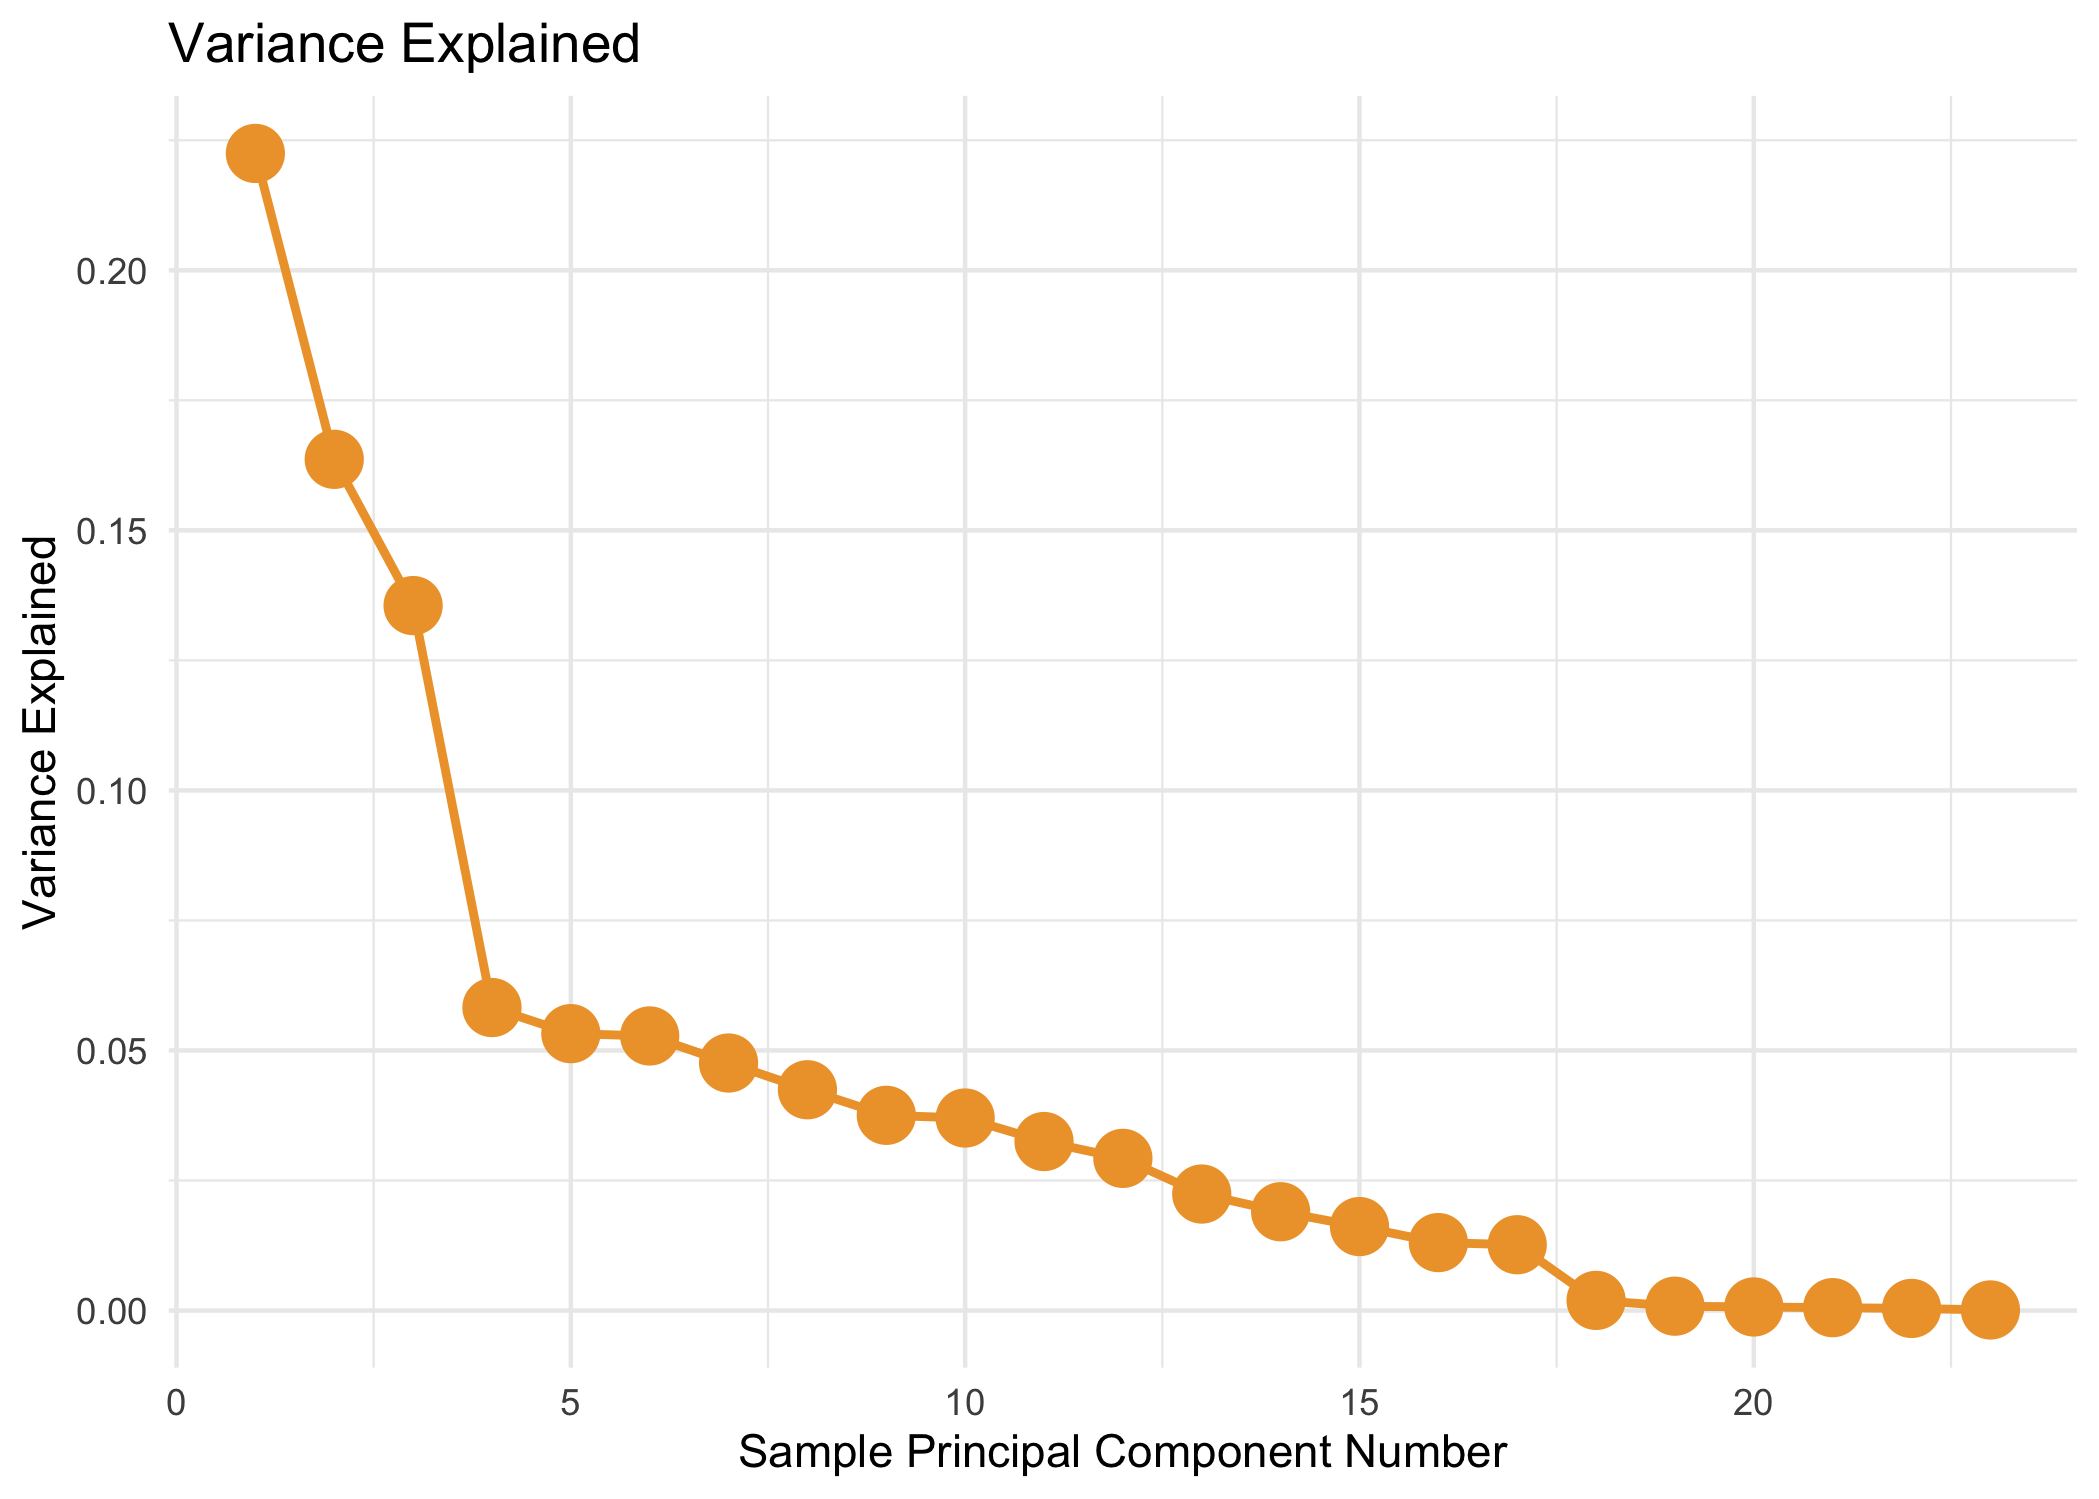
\includegraphics[height = 60mm, width=70mm]{pca_LR_scree.png}}\hspace{4em}
\subcaptionbox*{}{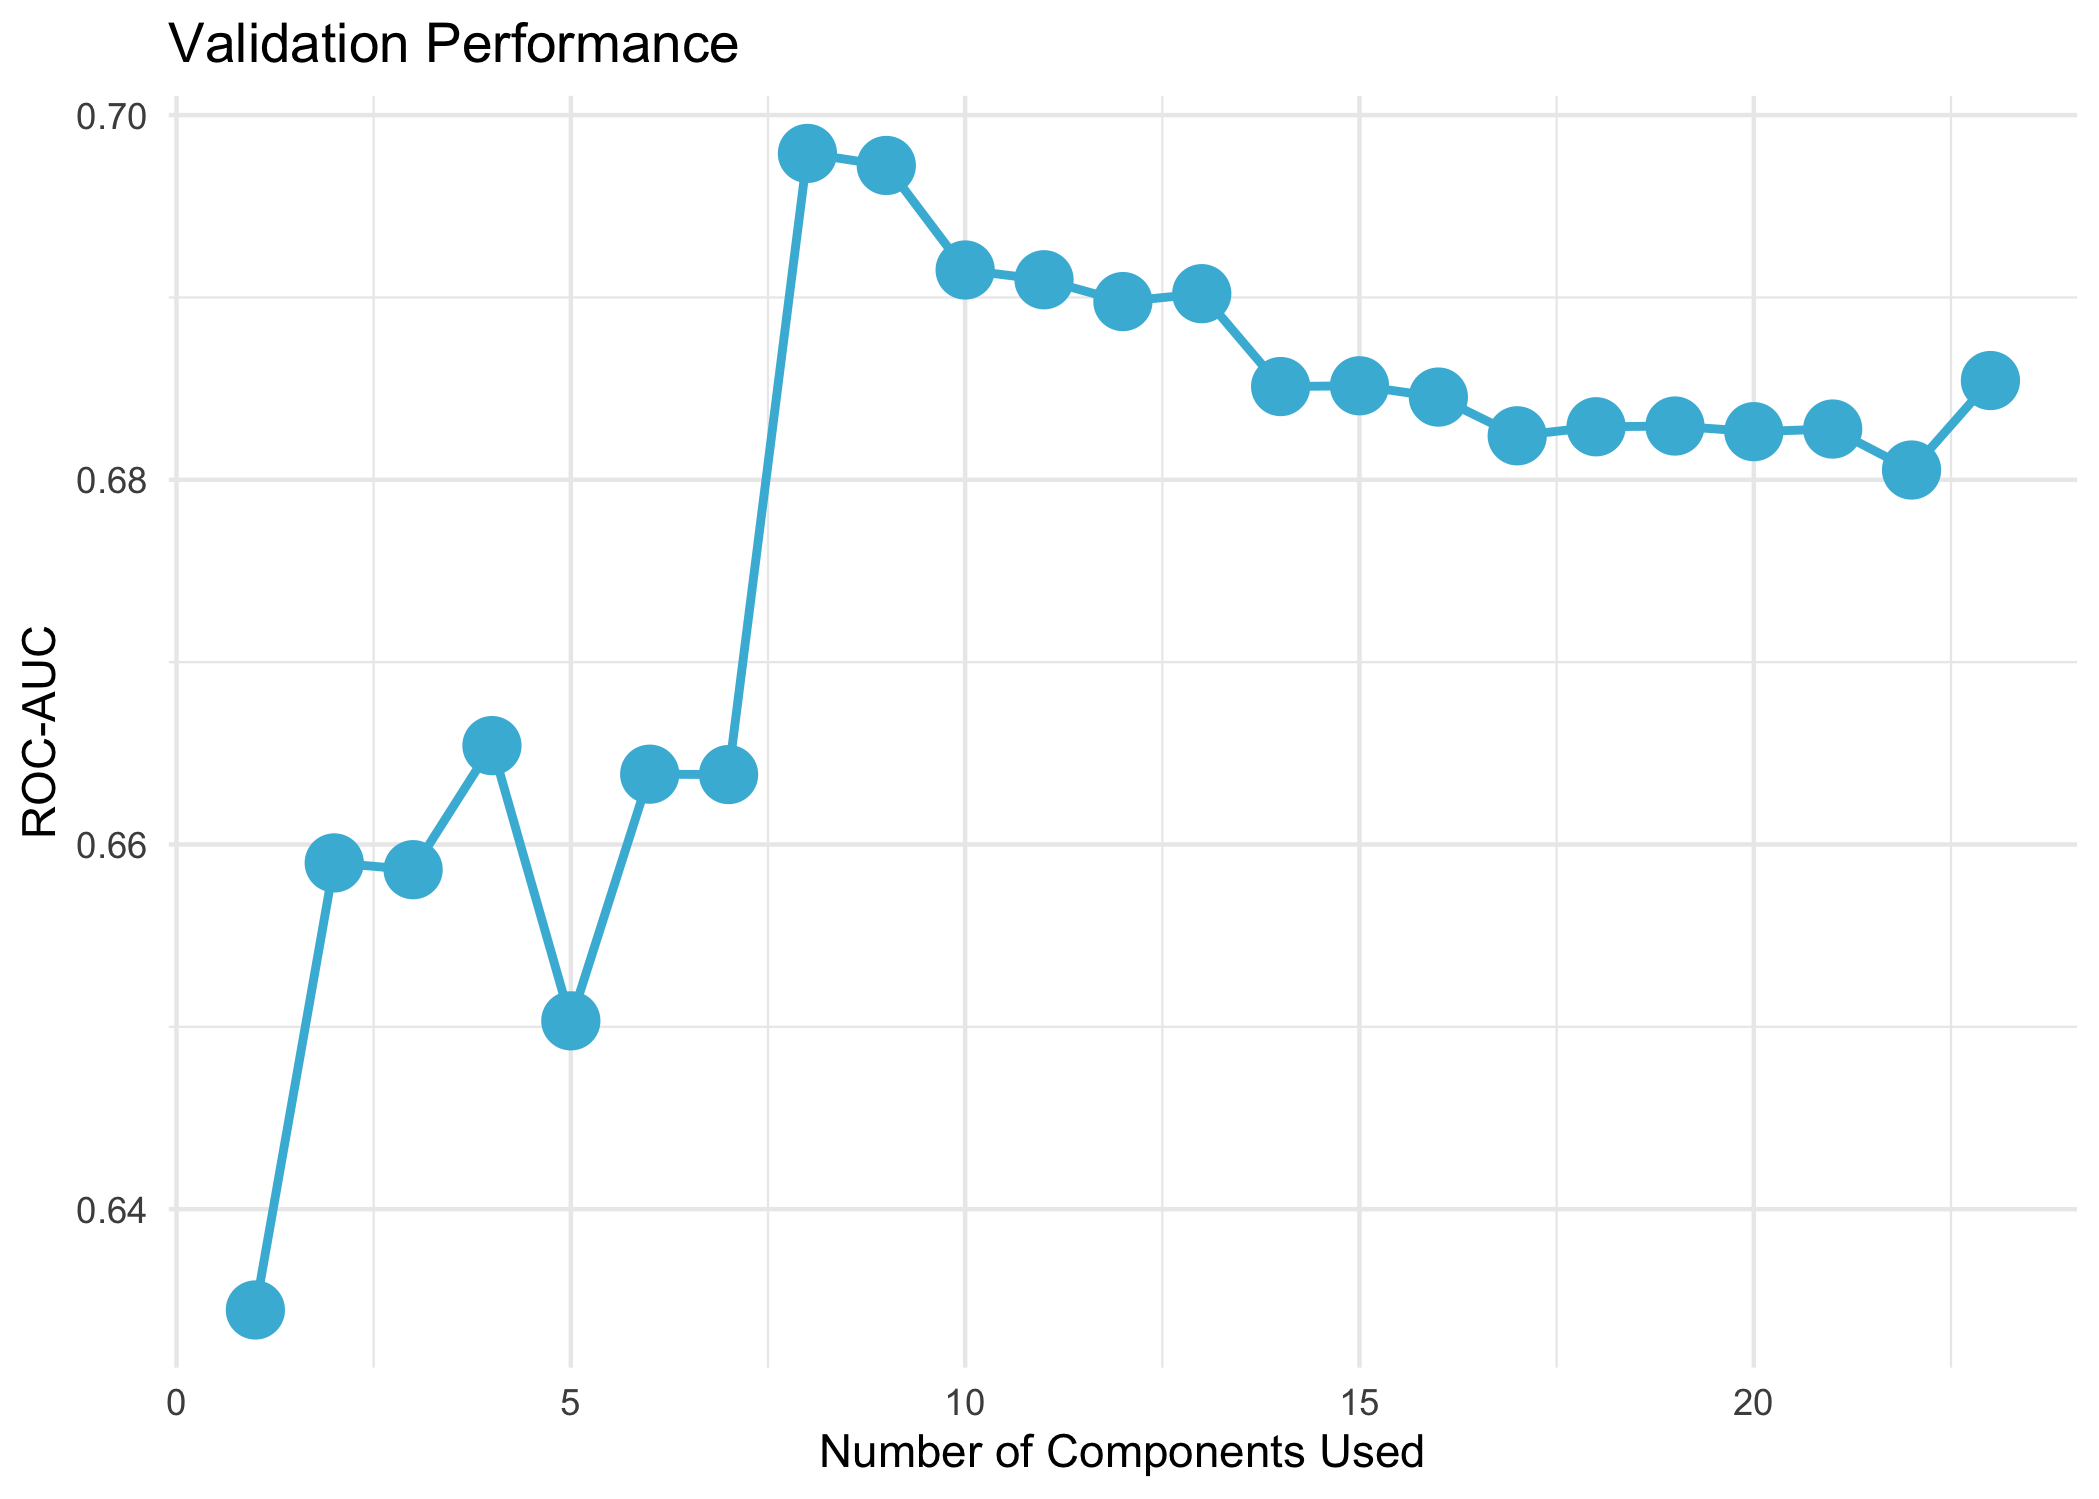
\includegraphics[height = 60mm, width=70mm]{pca_validation.png}}
\hspace*{\fill}
\end{figure}


We also found that $k = 8$ components provided the maximum ROC-AUC value of about 0.697 on our validation set. Since we know that $k=8$ components explain almost 80\% of the variance, and it achieves the best performance on our validation set, we trained our logistic regression model using the first $\hat{k}_{best} = 8$ sample principal components as input. 

\

Consequently, using the first 8 principal components reduced the dimension of the feature space from 23 to 8. We found that 6 out of the 8 components were significant at the $\alpha = 0.05$ level. We used residual deviance to test our model against the null model ($H_0: \beta_i = 0$ for all $i$). Again, we rejected the hypothesis and concluded that our new model demonstrated strong significance between the predictors and the response. The details of this test are shown in the table below.


\begin{table}[h!]
\centering
\begin{tabular}{| c | c | c | c | } 
\hline
& Resid. Df & Resid. Dev & Pr($>$Chi) \\ 
\hline
\hline
Null Model & 2340 & 3245.3 & \\
\hline
Model Using Predictors & 2332 & 2898.5 & $\approx 0$\\
\hline  
\end{tabular}
\end{table}

As we did with the previous model, we also assessed this model's fit by visually examining the Pearson Residuals vs Predicted Values plot and conducting a Pearson's $\chi^2$ goodness-of-fit test. The Pearson's $\chi^2$ goodness-of-fit test had a p-value of 0.30, so we rejected the hypothesis that our model did not fit the data well, and concluded that this model fits the data sufficiently well.


\subsubsection*{Logistic Regression with Elastic Net Regularization}

In our final logistic regression model, we used the (scaled) training and validation data to find the optimal mixing parameter, $\alpha$, and regularization parameter, $\lambda$. This process consisted of training our elastic net model with a variety of different pairs of mixing parameters ranging from $\alpha \in [0, 1]$ and $\lambda \in [0, 3]$, computing predictions for the validation set, and then comparing the corresponding ROC-AUC scores against each other. Ultimately, we found that the model with the best ROC-AUC (0.698) used a mixing percentage of $\hat{\alpha} = 0.6$ and a regularization parameter of $\hat{\lambda} = 0.098$. The plot below aided in our comparisons of ROC-AUC scores, and helped us determine the optimal hyper-parameters.


\begin{figure}[ht!]
\centering
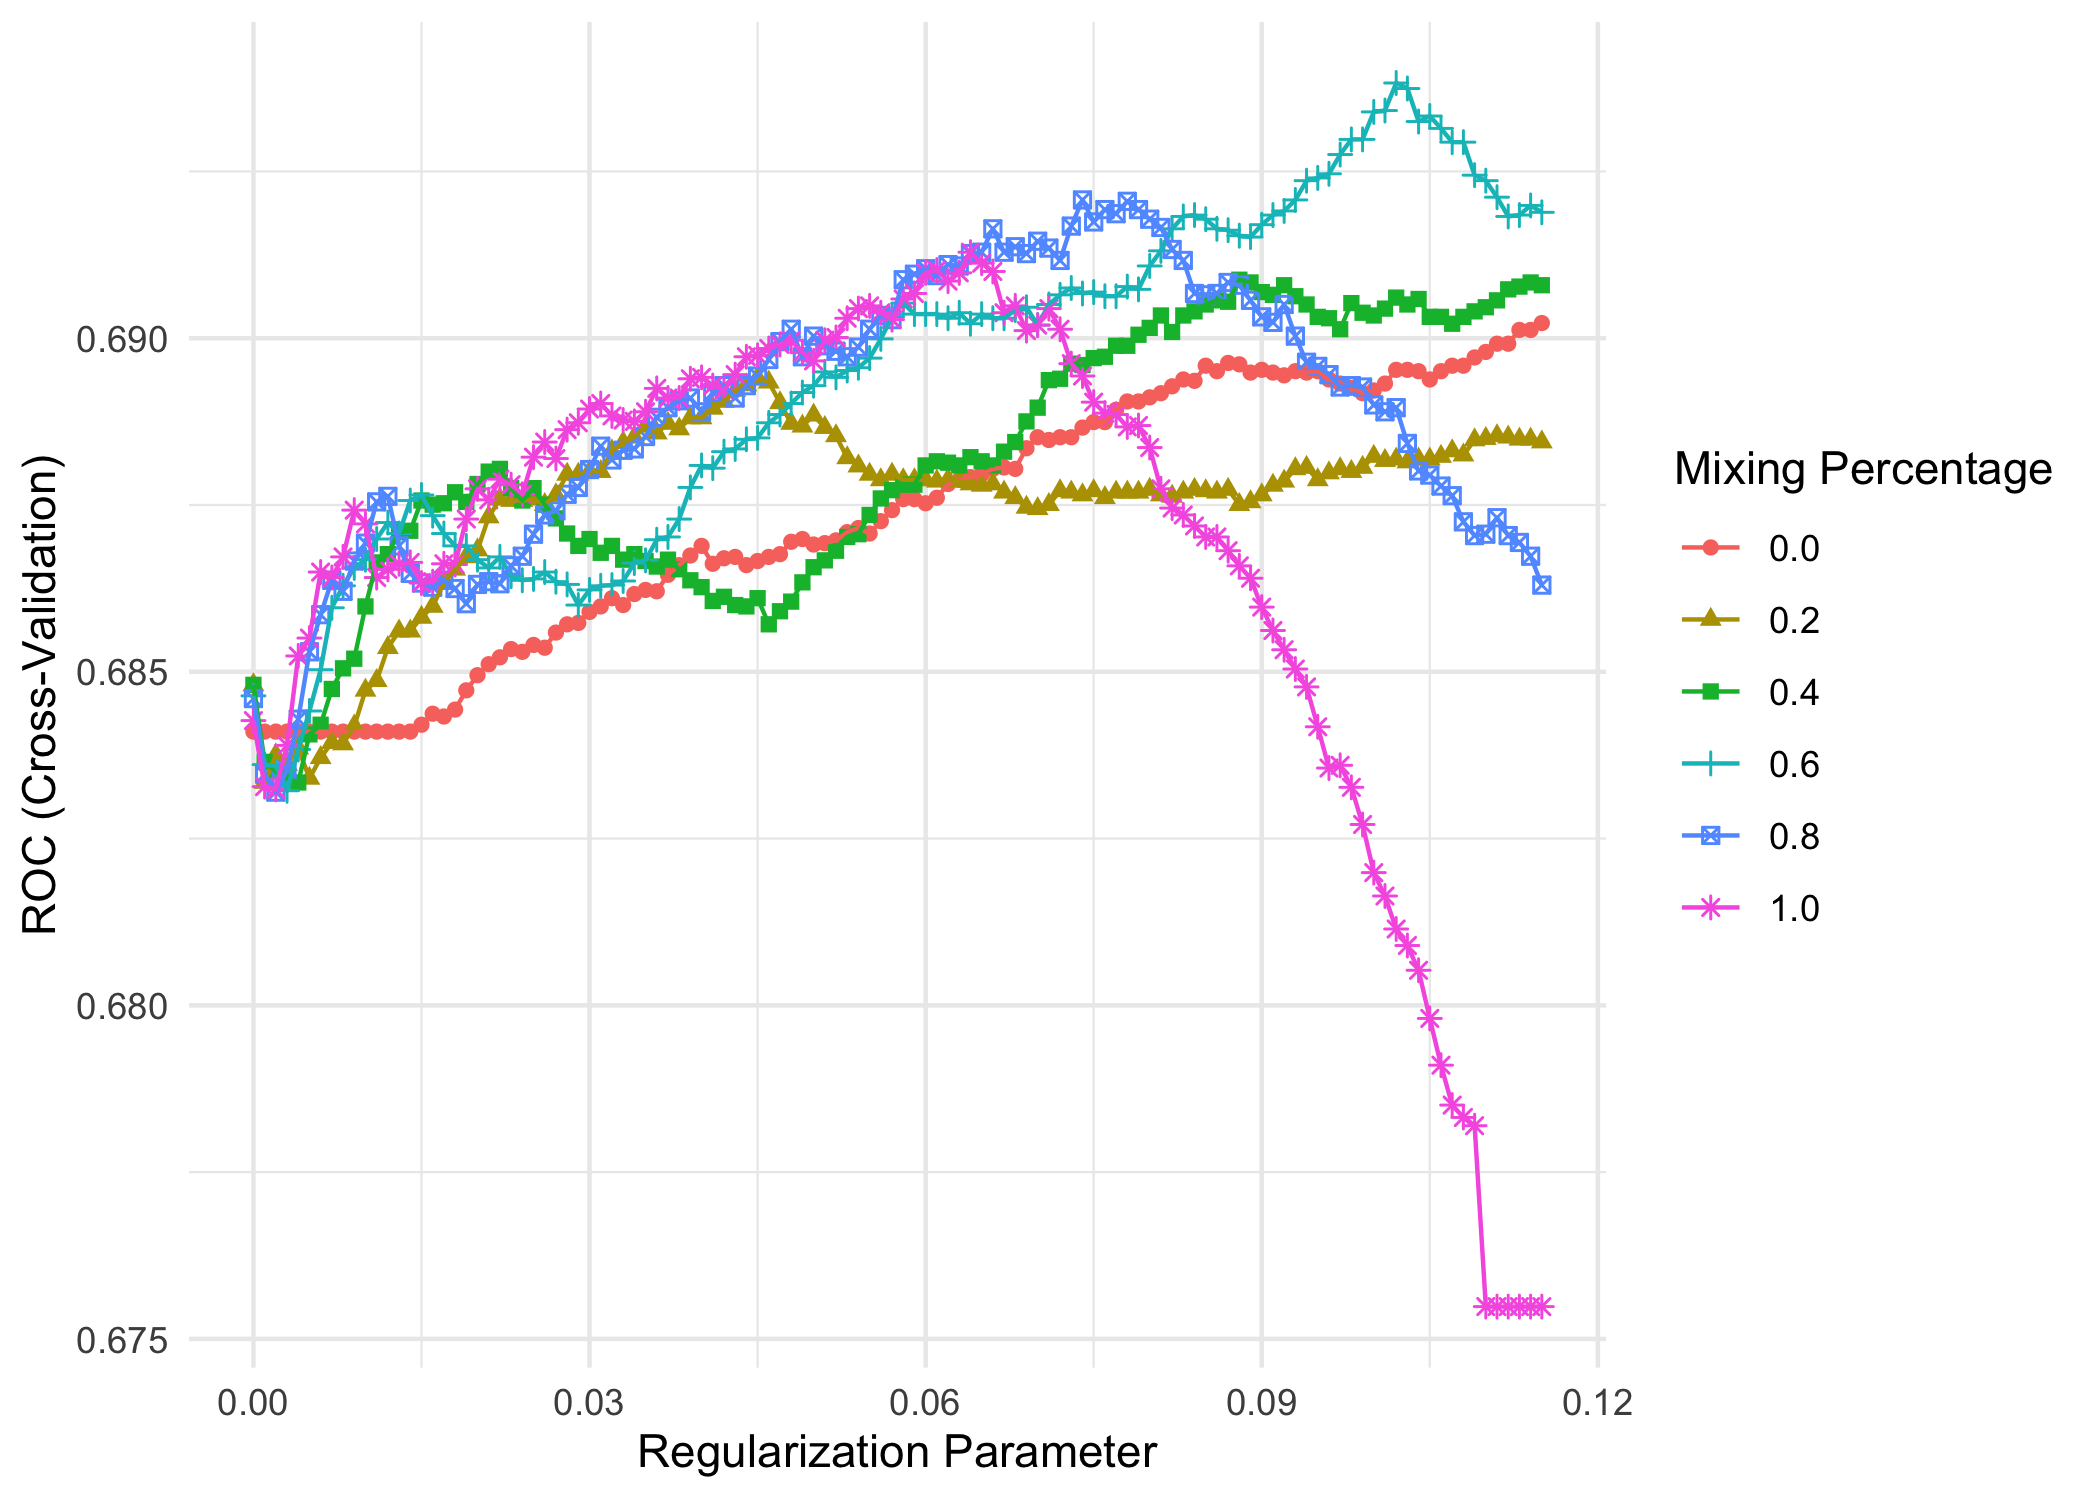
\includegraphics[height = 70mm, width=90mm]{elastic_LR_tuning.png}
\end{figure}

After obtaining $\hat{\alpha}$ and $\hat{\lambda}$, we trained our elastic net model one more time using both the training and the validation set. Interestingly, we found that this tuned elastic net model only retained 6 of the original predictors in its model. That is, the regularization effectively reduced the dimension of our feature space form 23 to 6, and the only remaining predictor variables with non-zero coefficients were: Gender, Age, Systolic Blood Pressure, $(\text{Systolic Blood Pressure})^2$, $(\text{Age} \cdot \text{Cigarettes Per Day})$, and $(\text{Systolic Blood Pressure} \cdot \text{Cigarettes Per Day})$. 

\

As shown in the previous models, the deviance for the elastic net model also indicated that the 6 remaining predictors demonstrated a significant relationship with the risk of heart disease. After visually inspecting the Pearson (and Deviance) Residuals vs Predicted Values plots, we found that this model exhibited a similar goodness-of-fit when compared to the previous two logistic regression models.

\subsubsection*{XGBoost}

Although this ensemble based model is very different from the previous three models, the approach for training, tuning, and validation remained similar. We used the associated ROC-AUC scores on the validation set to tune the depth of the trees and the number of trees to use in the XGBoost model. Similar to the elastic net model, we performed a ``grid-search'' for these two hyper-parameters which effectively trained an XGBoost model with a variety of different pairs of tree depths and numbers of trees. The ROC-AUC score for the validation set was then computed for each pair of hyper-parameters. The plot (left) below was used to find the optimal tree depth and number of trees. 

\

The optimal tree depth is clearly 2, and we can see that once the number of trees exceeds about 13, the ROC-AUC score reaches about 0.67 and then either plateaus or drops significantly. Therefore, to prevent potentially overfitting our data and to keep our model as simple as possible, we decided that the optimal number of trees is 13. Our final XGBoost model with 13 trees and a tree depth of 2 was re-trained on both the training and validation data.

\

Additionally, we used our XGBoost model to estimate each predictor variable's level of relative importance, or impact, on the model's predicted probabilities. These ordered levels of importance can be seen in the feature importance plot (right) shown below. The x-axis is a measure known as “Gain”. Gain is commonly described as the improvement in accuracy brought by the specific predictor to the branches (and trees) it is on \cite{xgbImp}. We can immediately see that our XGBoost model places significantly more importance on Age than it does on any other predictor. In fact, the predictor variables Age, Systolic Blood Pressure, and $(\text{Systolic Blood Pressure} \cdot \text{Cigarettes Per Day})$ all demonstrated significant importance in our XGBoost model. Notice that these results seem to agree with our elastic net model. The three most important variables in the XGBoost model are among the six remaining predictors in the elastic net model. 

\begin{figure}[hbt!]
\hspace*{\fill}
\centering
\subcaptionbox*{}{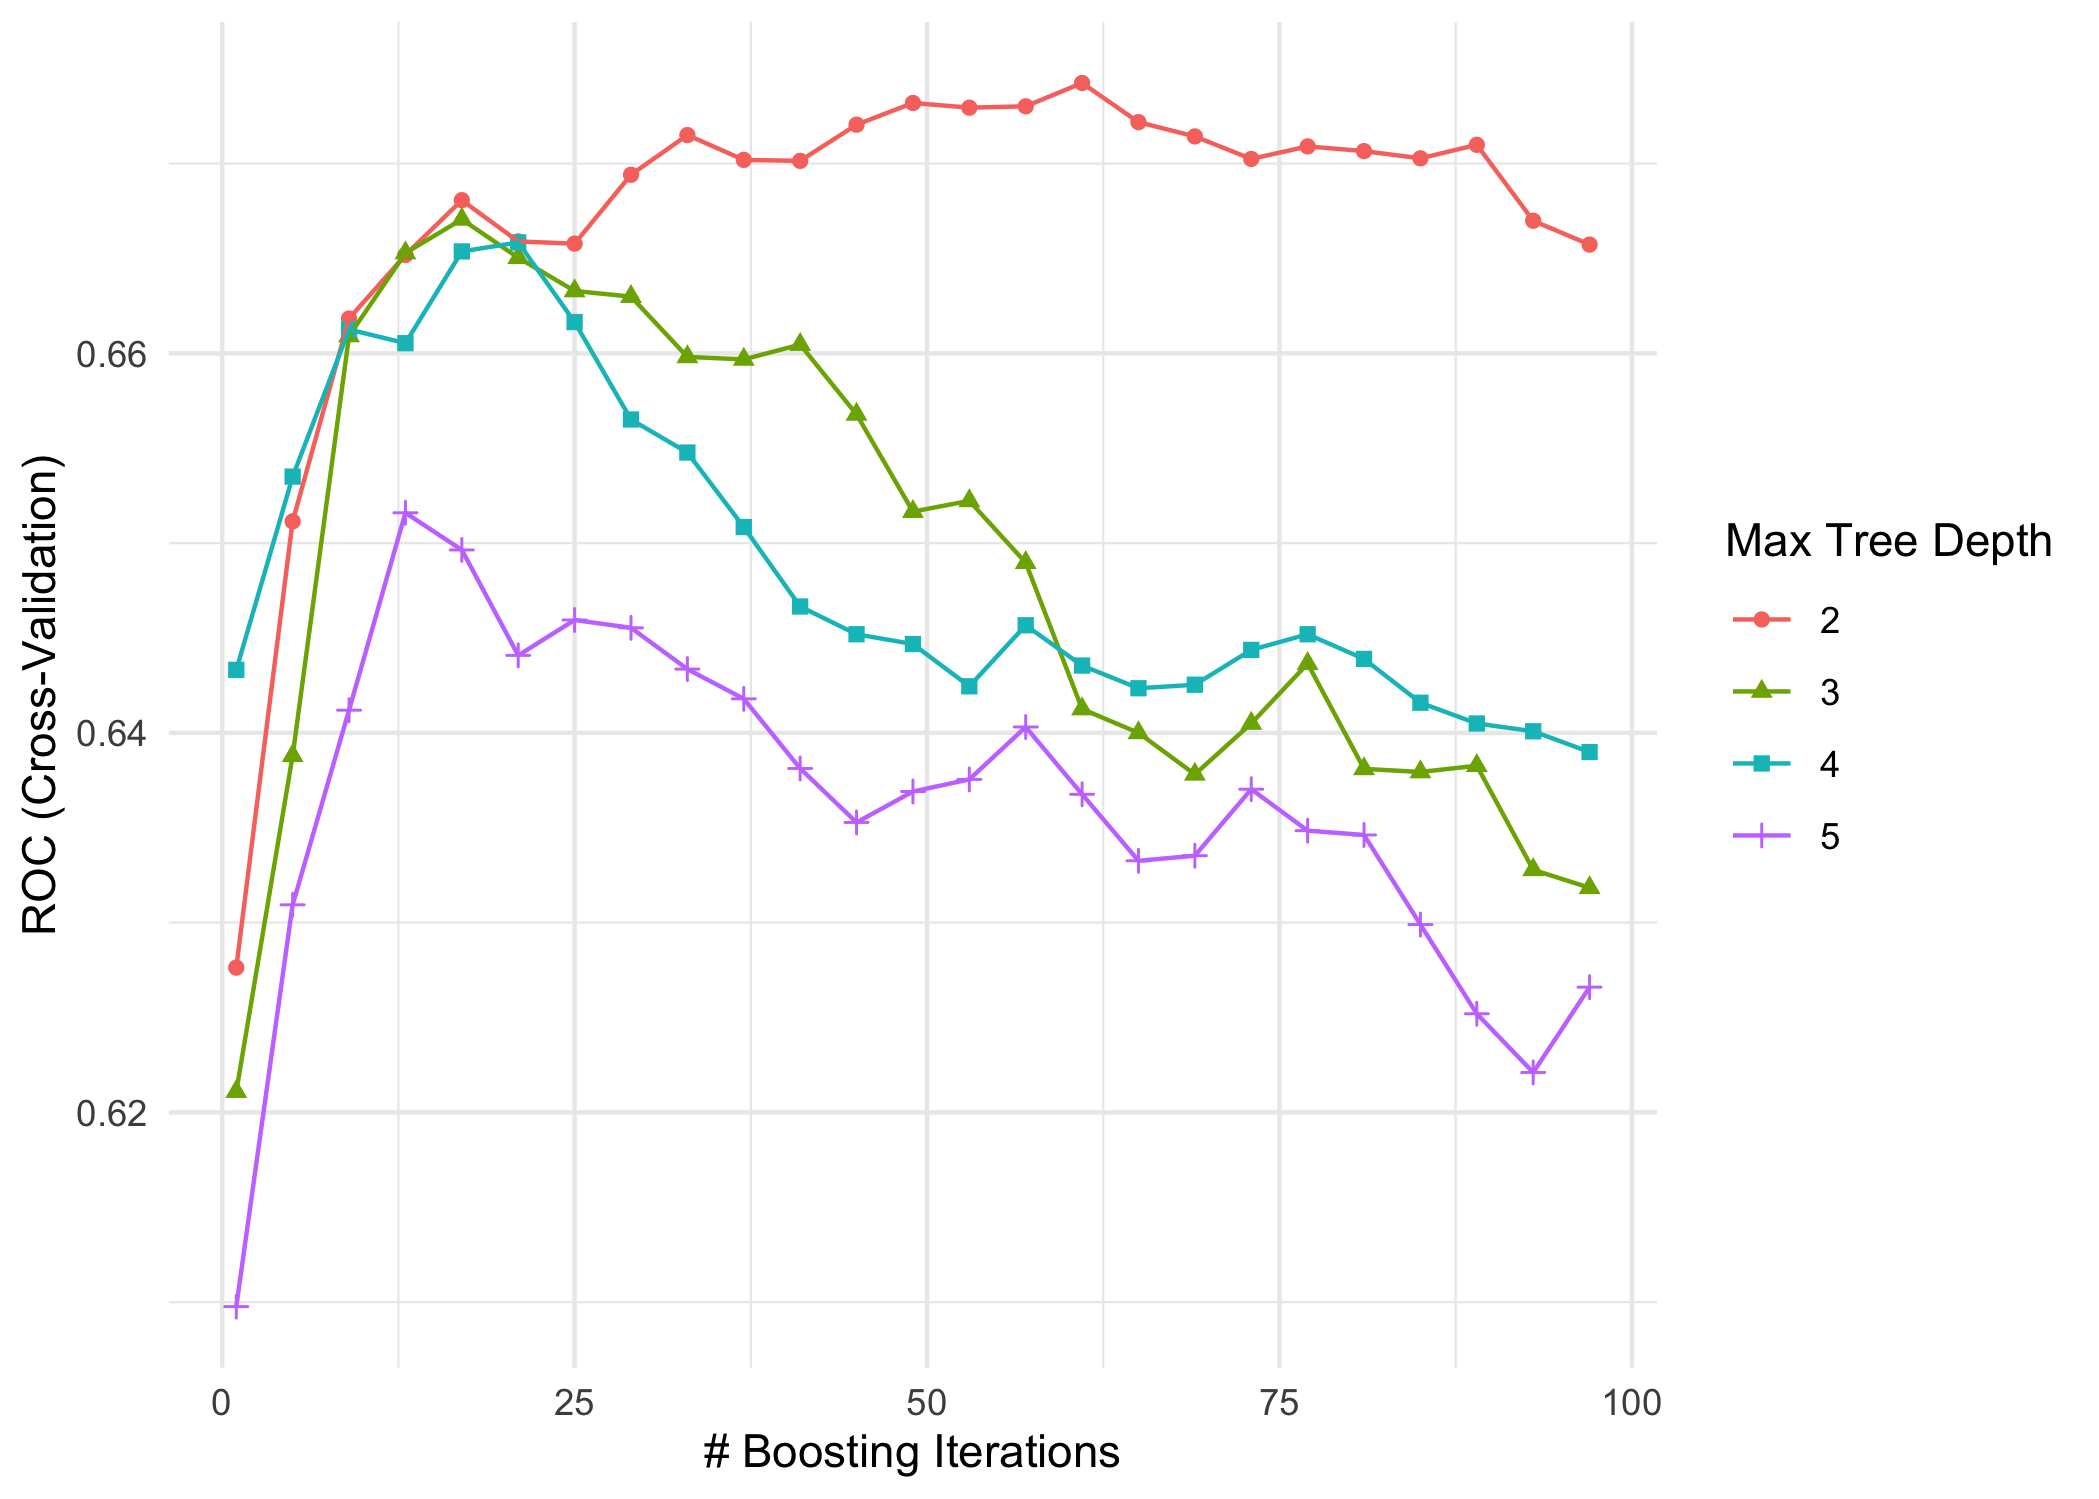
\includegraphics[height = 60mm, width=75mm]{xgb_tuning.png}}\hspace{0em}
\subcaptionbox*{}{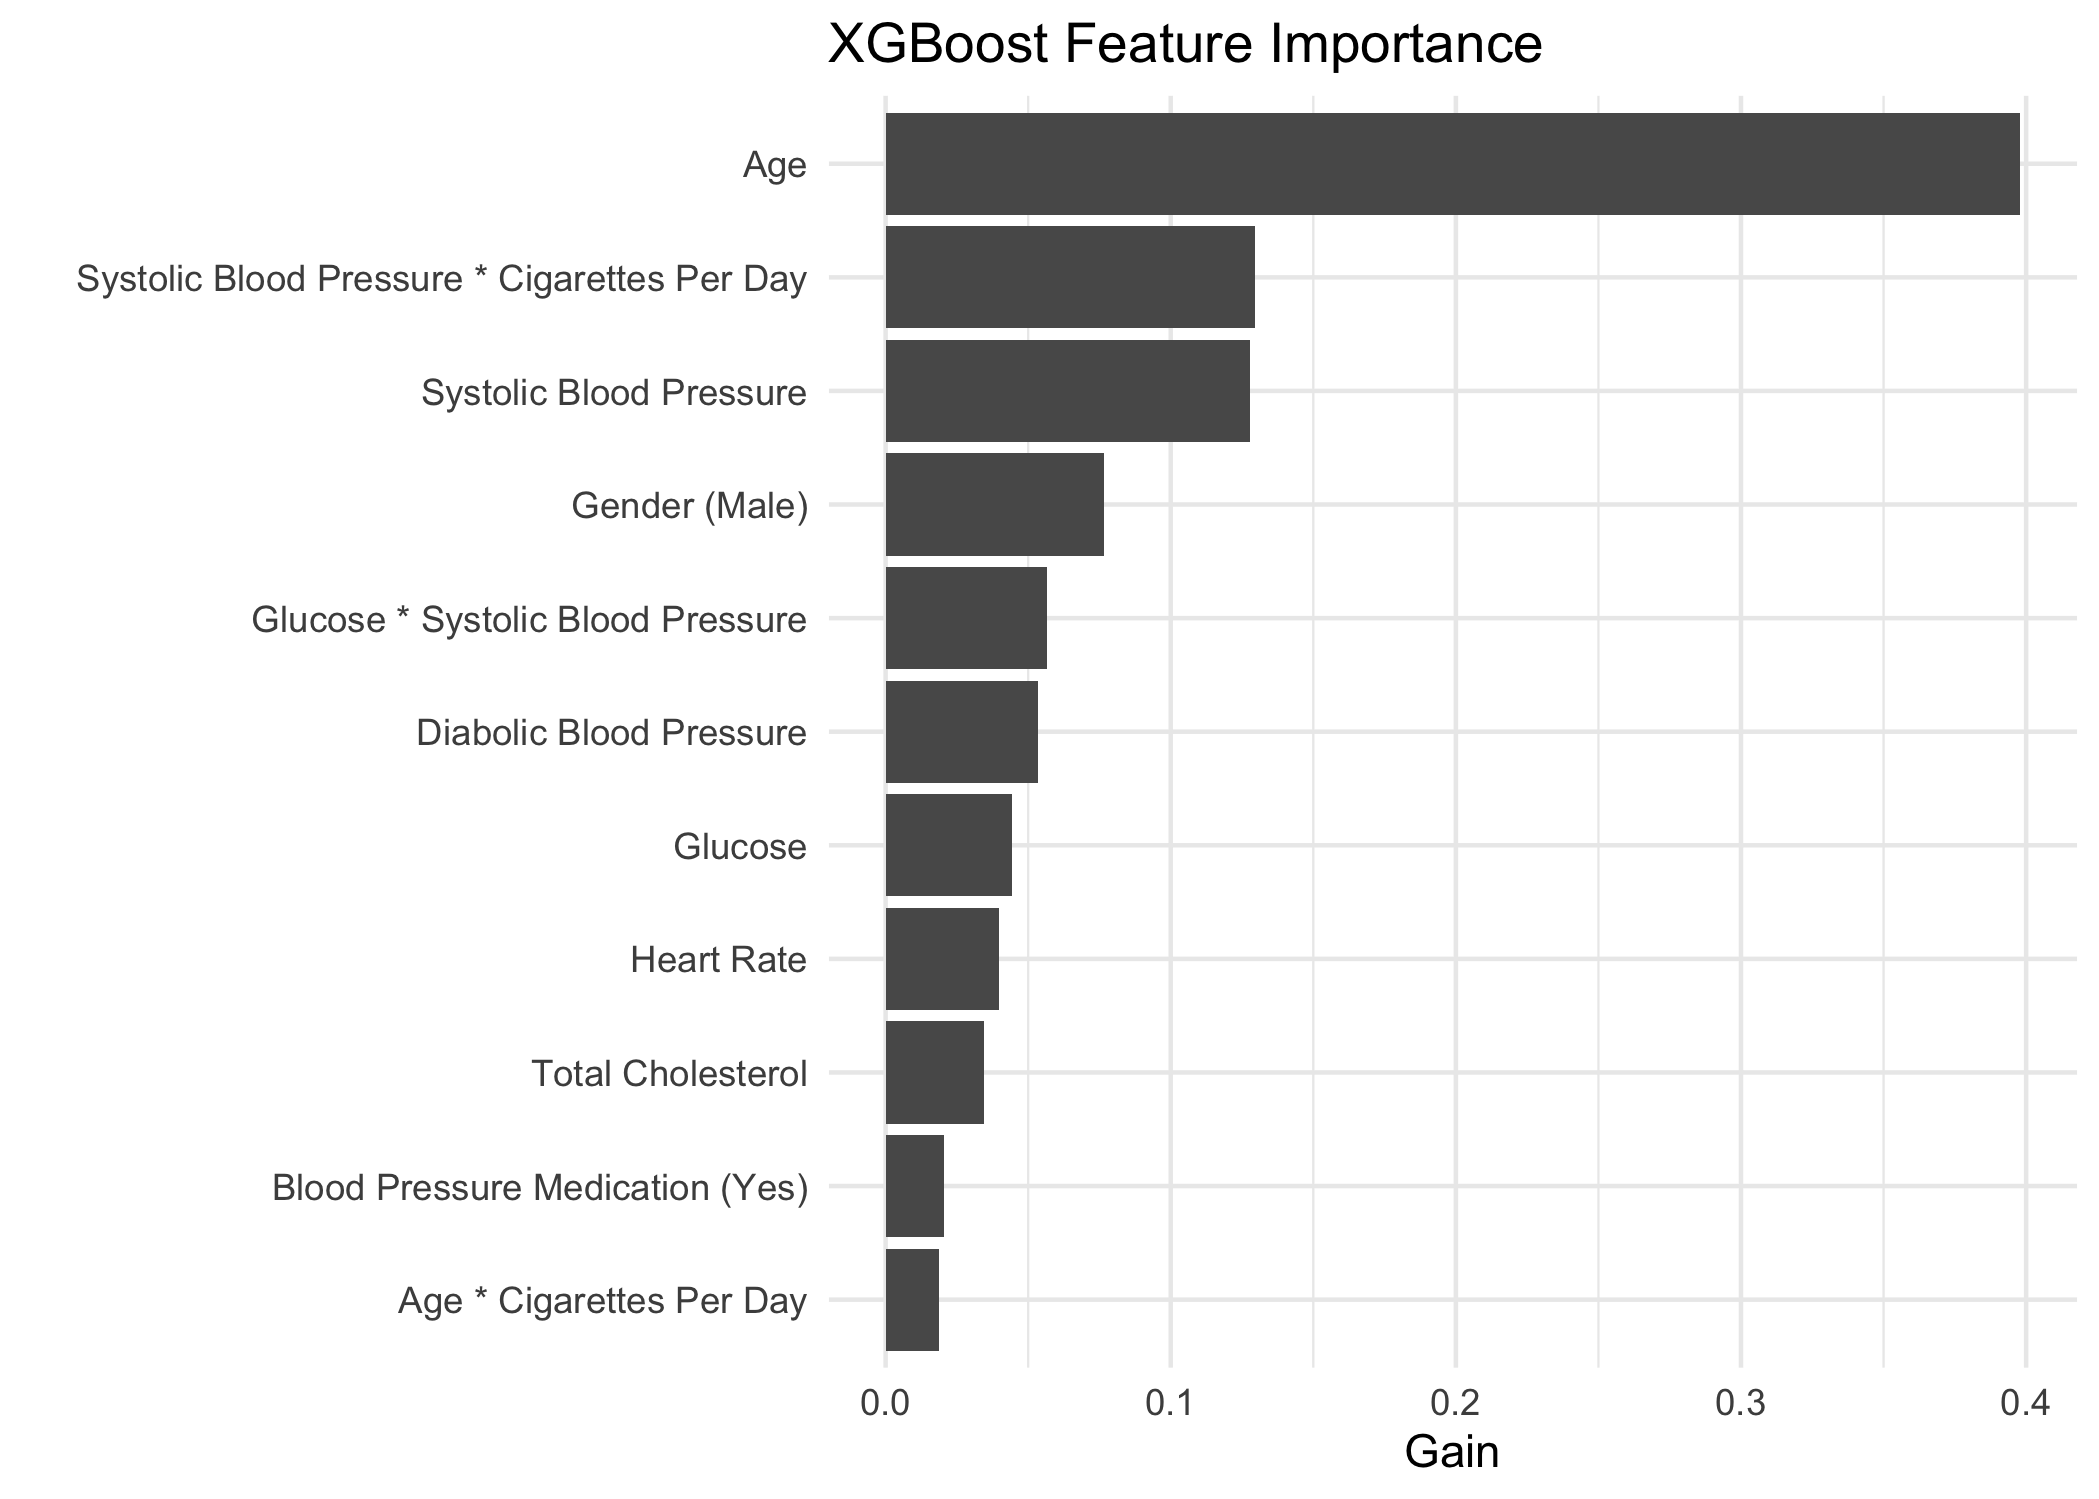
\includegraphics[height = 60mm, width=75mm]{xgb_importance.png}}
\hspace*{\fill}
\end{figure}

\subsubsection*{Model Evaluation and Comparison}

In this final results section, we use the dedicated test data to assess and compare the overall predictive performance of each model through a variety of metrics and visuals. We started by examining the metrics of interest over all possible thresholds. Recall that the metrics of interest are true-positive rate and true-negative rate as they are not influenced by the large class imbalance. That is, assessing performance with a measure like accuracy would not be appropriate in our case because a model that always classifies a patient as “not at risk of heart disease” would achieve an 85\% accuracy on our test set. Thus, we present the plots of sensitivity and specificity vs threshold:

\begin{figure}[hbt!]
\hspace*{\fill}
\centering
\subcaptionbox*{}{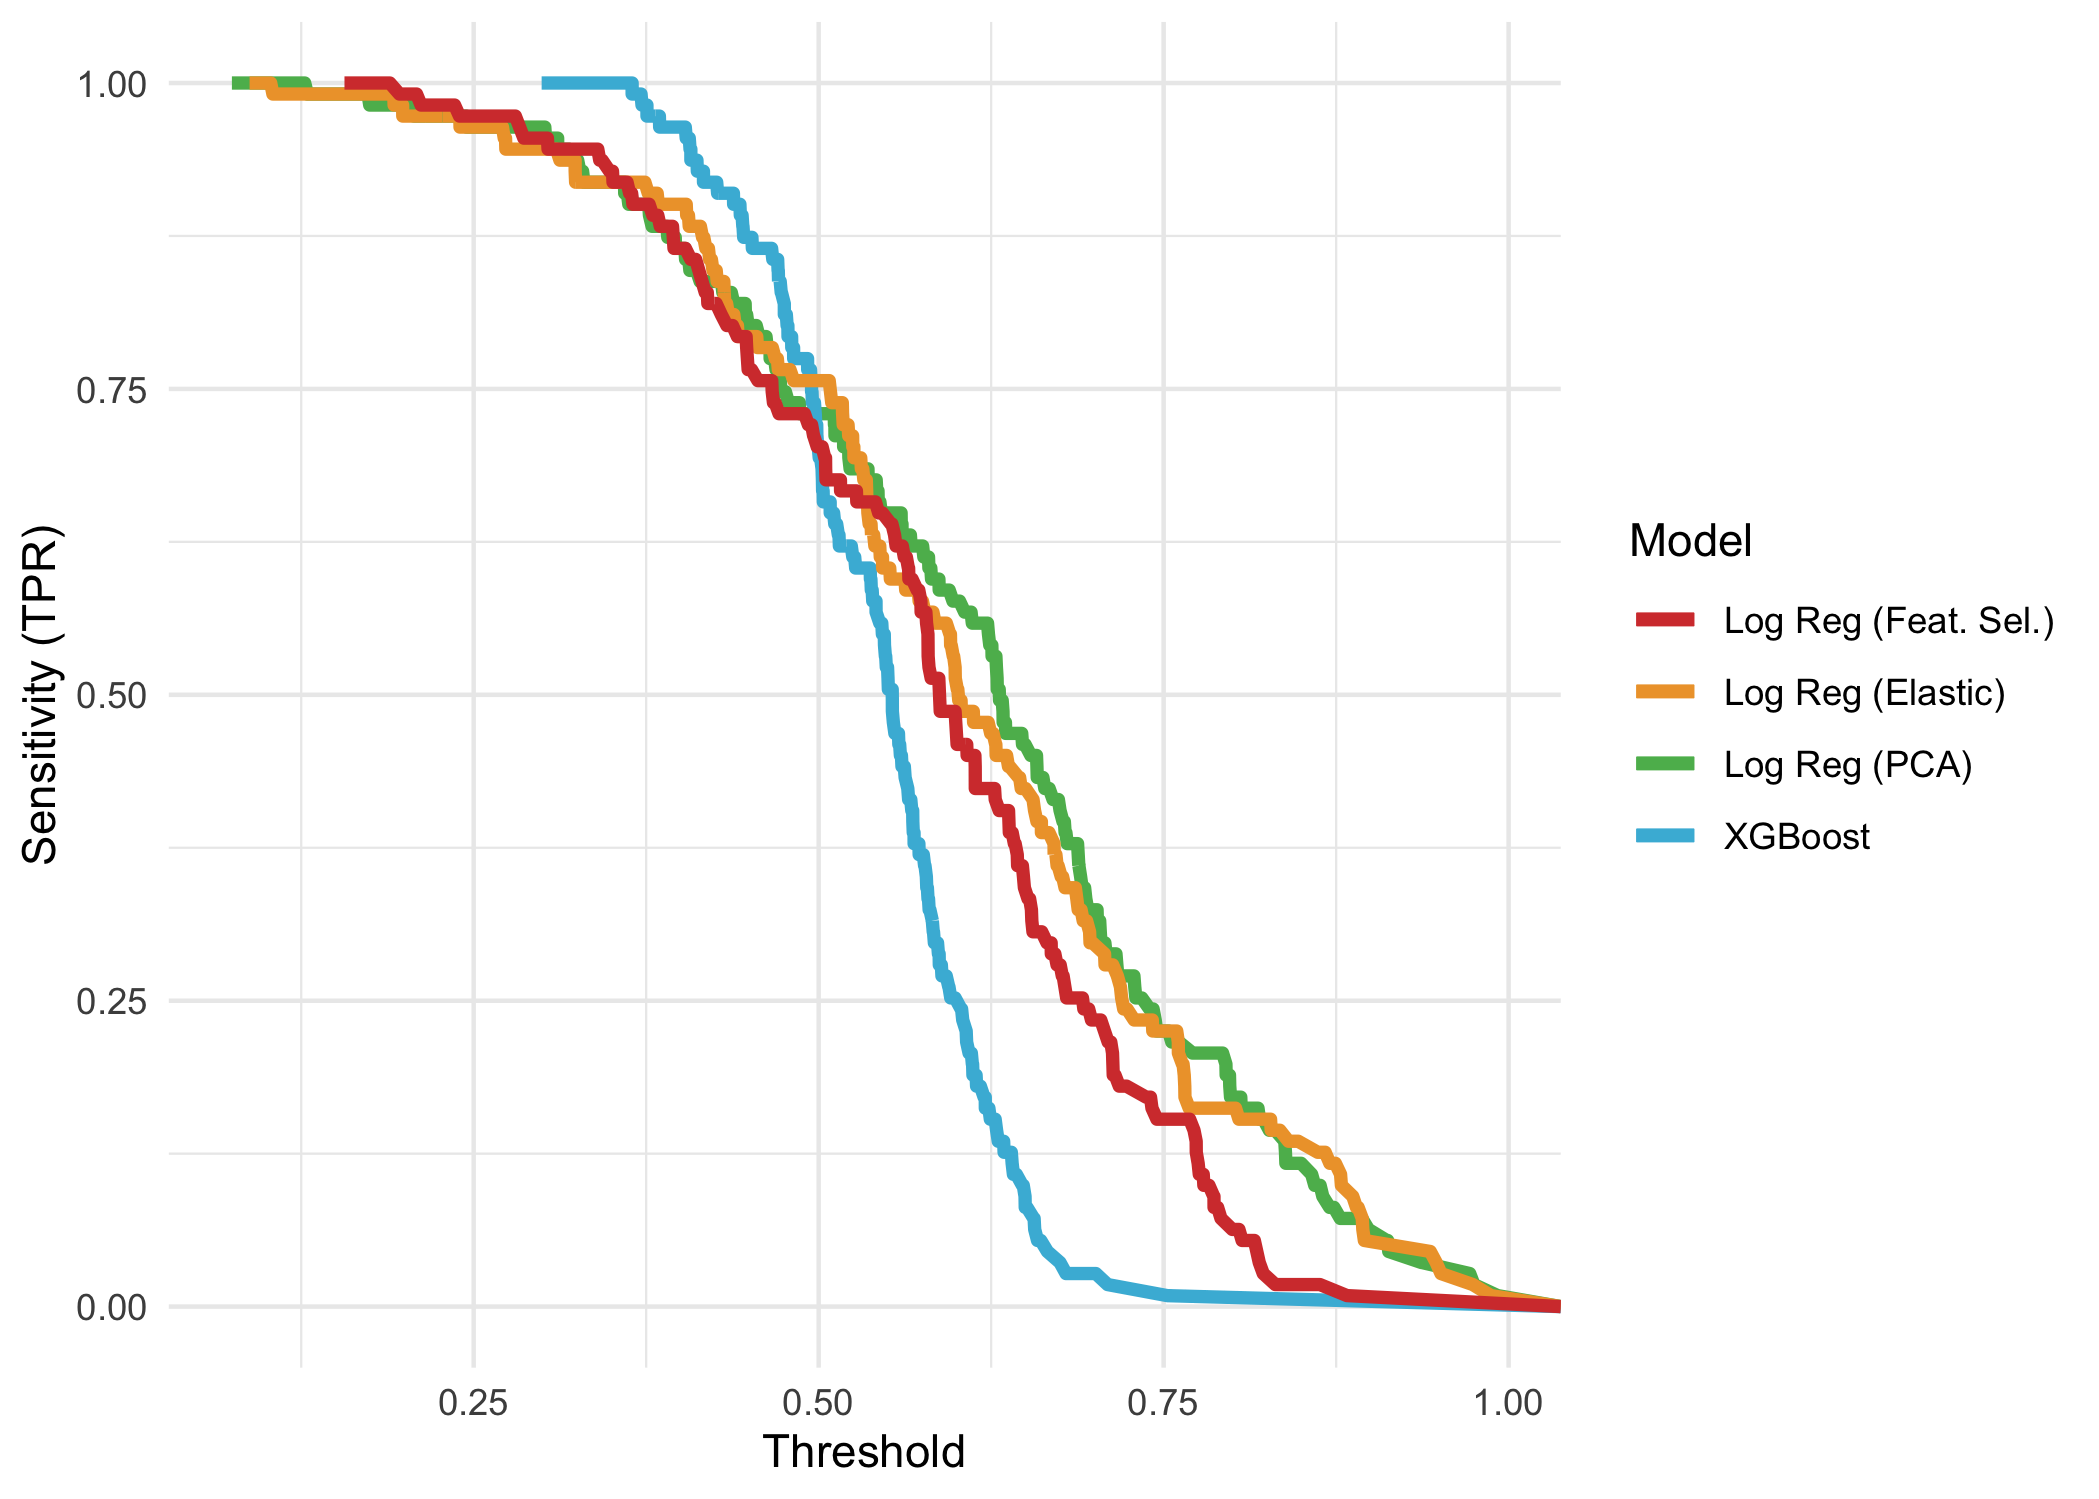
\includegraphics[height = 60mm, width=75mm]{results_sens.png}}\hspace{0em}
\subcaptionbox*{}{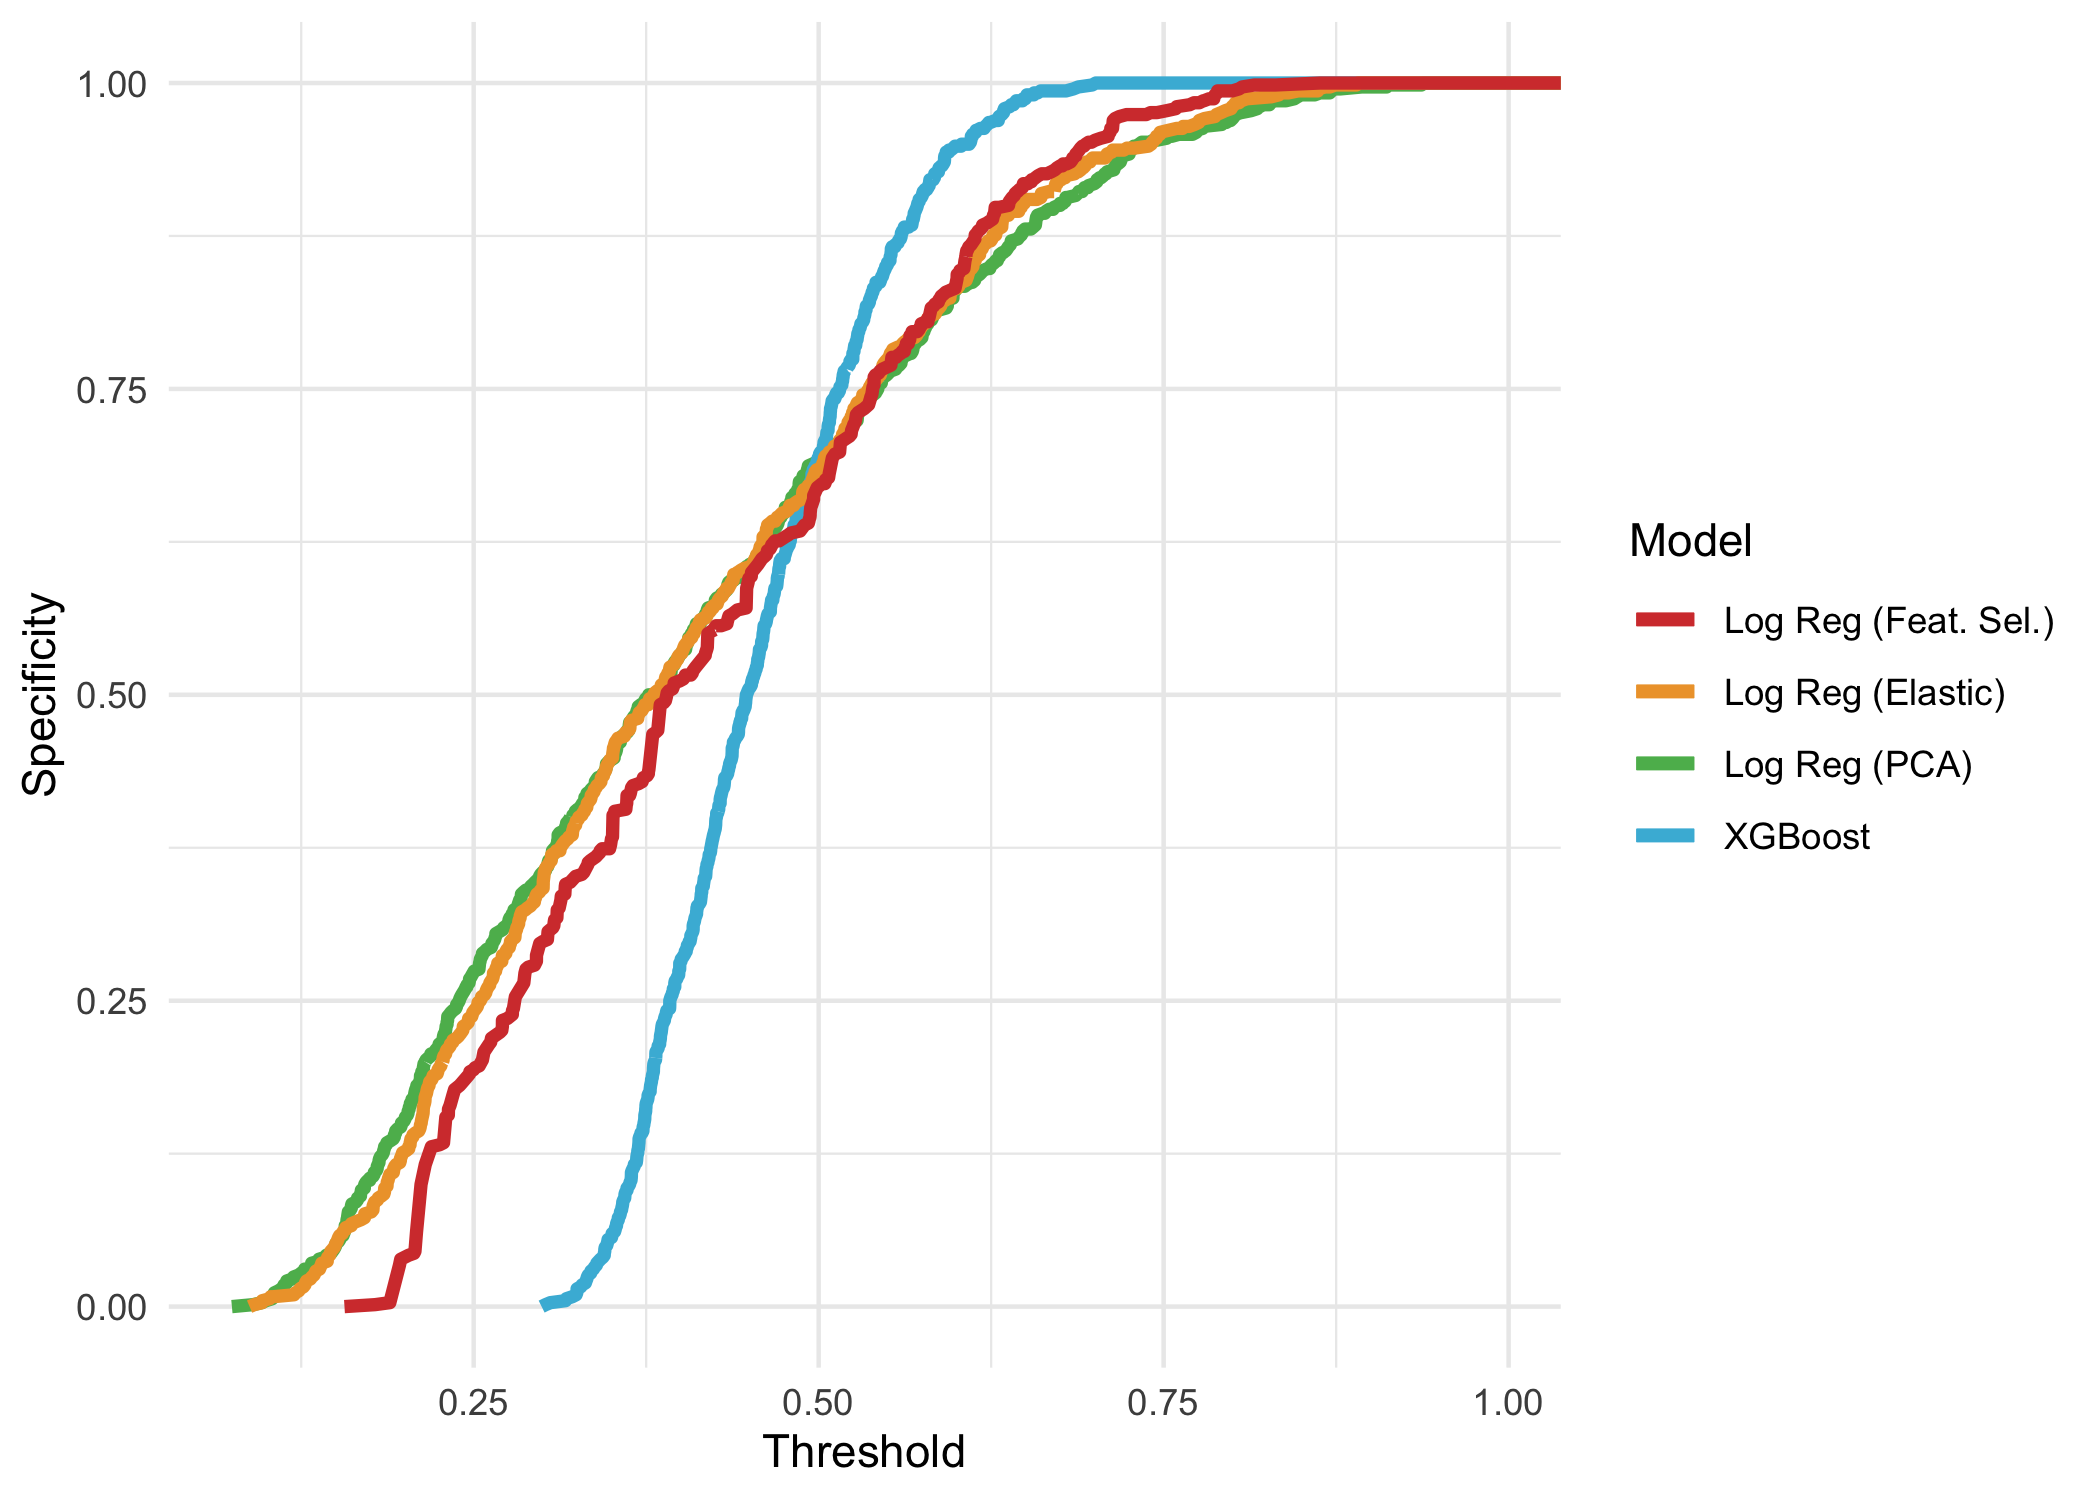
\includegraphics[height = 60mm, width=75mm]{results_spec.png}}
\hspace*{\fill}
\end{figure}

As we mentioned in previous sections, since our model is attempting to predict the presence of a life-threatening condition, a false-negative is far more dangerous than a false-positive. Ideally, we wanted the model to have the greatest true-positive rate possible without compromising the overall “trust” in its classifications. That is, our goal was to maximize the sensitivity without dropping the specificity too much. The plots above indicate that there exists a range of thresholds between 0.4 to 0.6 that could accomplish this goal. Notice that since the curves for the XGBoost model are much steeper than the curves for the logistic regression models, this optimal range of thresholds may be a bit smaller for the XGBoost model than it is for the three logistic regression models.

\

As mentioned in the methodology section, we used the geometric mean of the sensitivity and the specificity to find the optimal threshold, $t^*$, for each model. We evaluated the $G_{mean}(t)$ at a variety of different thresholds between $t \in [0.4, 0.6]$, and stored the threshold that maximized the $G_{mean}(t)$. Using the optimal thresholds for each model, we created the following performance metrics and confusion matrices from our test set:

\begin{table}[h!]
\centering
\begin{tabular}{| c | c | c | c | } 
\hline
Model & Sensitivity & Specificity & Balanced Accuracy \\ 
\hline
\hline
Logistic Regression (with Feat. Sel.) & 0.802 & 0.608 & 0.705\\
\hline
Logistic Regression (with PCA) & 0.739 & 0.700 & 0.719\\
\hline
Logistic Regression (with Elastic Net) & 0.775 & 0.661 & 0.718\\
\hline  
XGBoost & 0.703 & 0.673 & 0.688\\
\hline  
\end{tabular}
\end{table}

\begin{table}[hbt!]
\begin{subtable}{.5\linewidth}\centering
{\begin{tabular}{cc|c|c|c|}
    &\multicolumn{1}{c}{}&\multicolumn{3}{c}{\textbf{Predicted}}\\
    &\multicolumn{1}{c}{}&\multicolumn{1}{c}{\textbf{No Risk}}
    &\multicolumn{1}{c}{\textbf{Risk}}
    &\multicolumn{1}{c}{\textbf{Total}}\\
    \cline{3-5}
    \multicolumn{1}{c}{\multirow{3}{*}{\rotatebox{90}{\textbf{Actual}}}}
    &\textbf{No Risk} &377 &243 &620\\
    \cline{3-5}
    &\textbf{Risk} &22 &89 &111\\
    \cline{3-5}
    &\textbf{Total} &399 &332 &\\
    \cline{3-5}
    \end{tabular}}
\caption{Log. Reg. w/ Feature Sel.}
\end{subtable}%
\begin{subtable}{.5\linewidth}\centering
{\begin{tabular}{cc|c|c|c|}
    &\multicolumn{1}{c}{}&\multicolumn{3}{c}{\textbf{Predicted}}\\
    &\multicolumn{1}{c}{}&\multicolumn{1}{c}{\textbf{No Risk}}
    &\multicolumn{1}{c}{\textbf{Risk}}
    &\multicolumn{1}{c}{\textbf{Total}}\\
    \cline{3-5}
    \multicolumn{1}{c}{\multirow{3}{*}{\rotatebox{90}{\textbf{Actual}}}}
    &\textbf{No Risk} &410 &210 &620\\
    \cline{3-5}
    &\textbf{Risk} &25 &86 &111\\
    \cline{3-5}
    &\textbf{Total} &435 &296 &\\
    \cline{3-5}
    \end{tabular}}
\caption{Log. Reg. w/ Elastic Net}
\end{subtable}
\begin{subtable}{.5\linewidth}\centering
    {\begin{tabular}{cc|c|c|c|}
        &\multicolumn{1}{c}{}&\multicolumn{3}{c}{\textbf{Predicted}}\\
        &\multicolumn{1}{c}{}&\multicolumn{1}{c}{\textbf{No Risk}}
        &\multicolumn{1}{c}{\textbf{Risk}}
        &\multicolumn{1}{c}{\textbf{Total}}\\
        \cline{3-5}
        \multicolumn{1}{c}{\multirow{3}{*}{\rotatebox{90}{\textbf{Actual}}}}
        &\textbf{No Risk} &434 &186 &620\\
        \cline{3-5}
        &\textbf{Risk} &29 &82 &111\\
        \cline{3-5}
        &\textbf{Total} &463 &268 &\\
        \cline{3-5}
        \end{tabular}}
    \caption{Log. Reg. w/ PCA}
    \end{subtable}%
    \begin{subtable}{.5\linewidth}\centering
    {\begin{tabular}{cc|c|c|c|}
        &\multicolumn{1}{c}{}&\multicolumn{3}{c}{\textbf{Predicted}}\\
        &\multicolumn{1}{c}{}&\multicolumn{1}{c}{\textbf{No Risk}}
        &\multicolumn{1}{c}{\textbf{Risk}}
        &\multicolumn{1}{c}{\textbf{Total}}\\
        \cline{3-5}
        \multicolumn{1}{c}{\multirow{3}{*}{\rotatebox{90}{\textbf{Actual}}}}
        &\textbf{No Risk} &417 &203 &620\\
        \cline{3-5}
        &\textbf{Risk} &33 &78 &111\\
        \cline{3-5}
        &\textbf{Total} &450 &281 &\\
        \cline{3-5}
        \end{tabular}}
    \caption{XGBoost}
    \end{subtable}
\caption*{Figure: Confusion Matrix For Each Model}
\end{table}


From the performance metrics and confusion matrices above, we can see that all four models demonstrate a good classification performance. More specifically, the logistic regression model using principal component analysis for dimension reduction and the logistic regression model using elastic net regularization demonstrate the best combinations of sensitivity and specificity. Both of these models achieve similar balanced accuracies at approximately 0.72 and clearly do a great job of distinguishing between patients with and without a 10-year risk of heart disease. It's important to note that the elastic net regression model only needed 6 predictors (the smallest feature space) to achieve such an excellent score on the test set.

\

For a more general assessment and comparison across all possible thresholds, we also used the testing data to compute the ROC curves for each model (shown below) and their associated ROC-AUCs.

\

\begin{figure}[hbt!]
\hspace*{\fill}
\centering
\subcaptionbox*{}{\begin{tabular}{| c | c |} 
    \hline
    & \\
    Model & ROC-AUC \\ 
    & \\
    \hline
    & \\
    \makecell{Logistic Regression \\ with Feat. Sel.} & 0.785\\
    & \\
    \hline
    & \\
    \makecell{Logistic Regression \\ with PCA} & 0.778\\
    & \\
    \hline
    & \\
    \makecell{Logistic Regression \\ with Elastic Net} & 0.784\\
    & \\
    \hline 
    & \\
    \makecell{eXtreme Gradient \\ Boosting} & 0.766\\
    & \\
    \hline
    \end{tabular}}\hspace{3em}
\subcaptionbox*{}{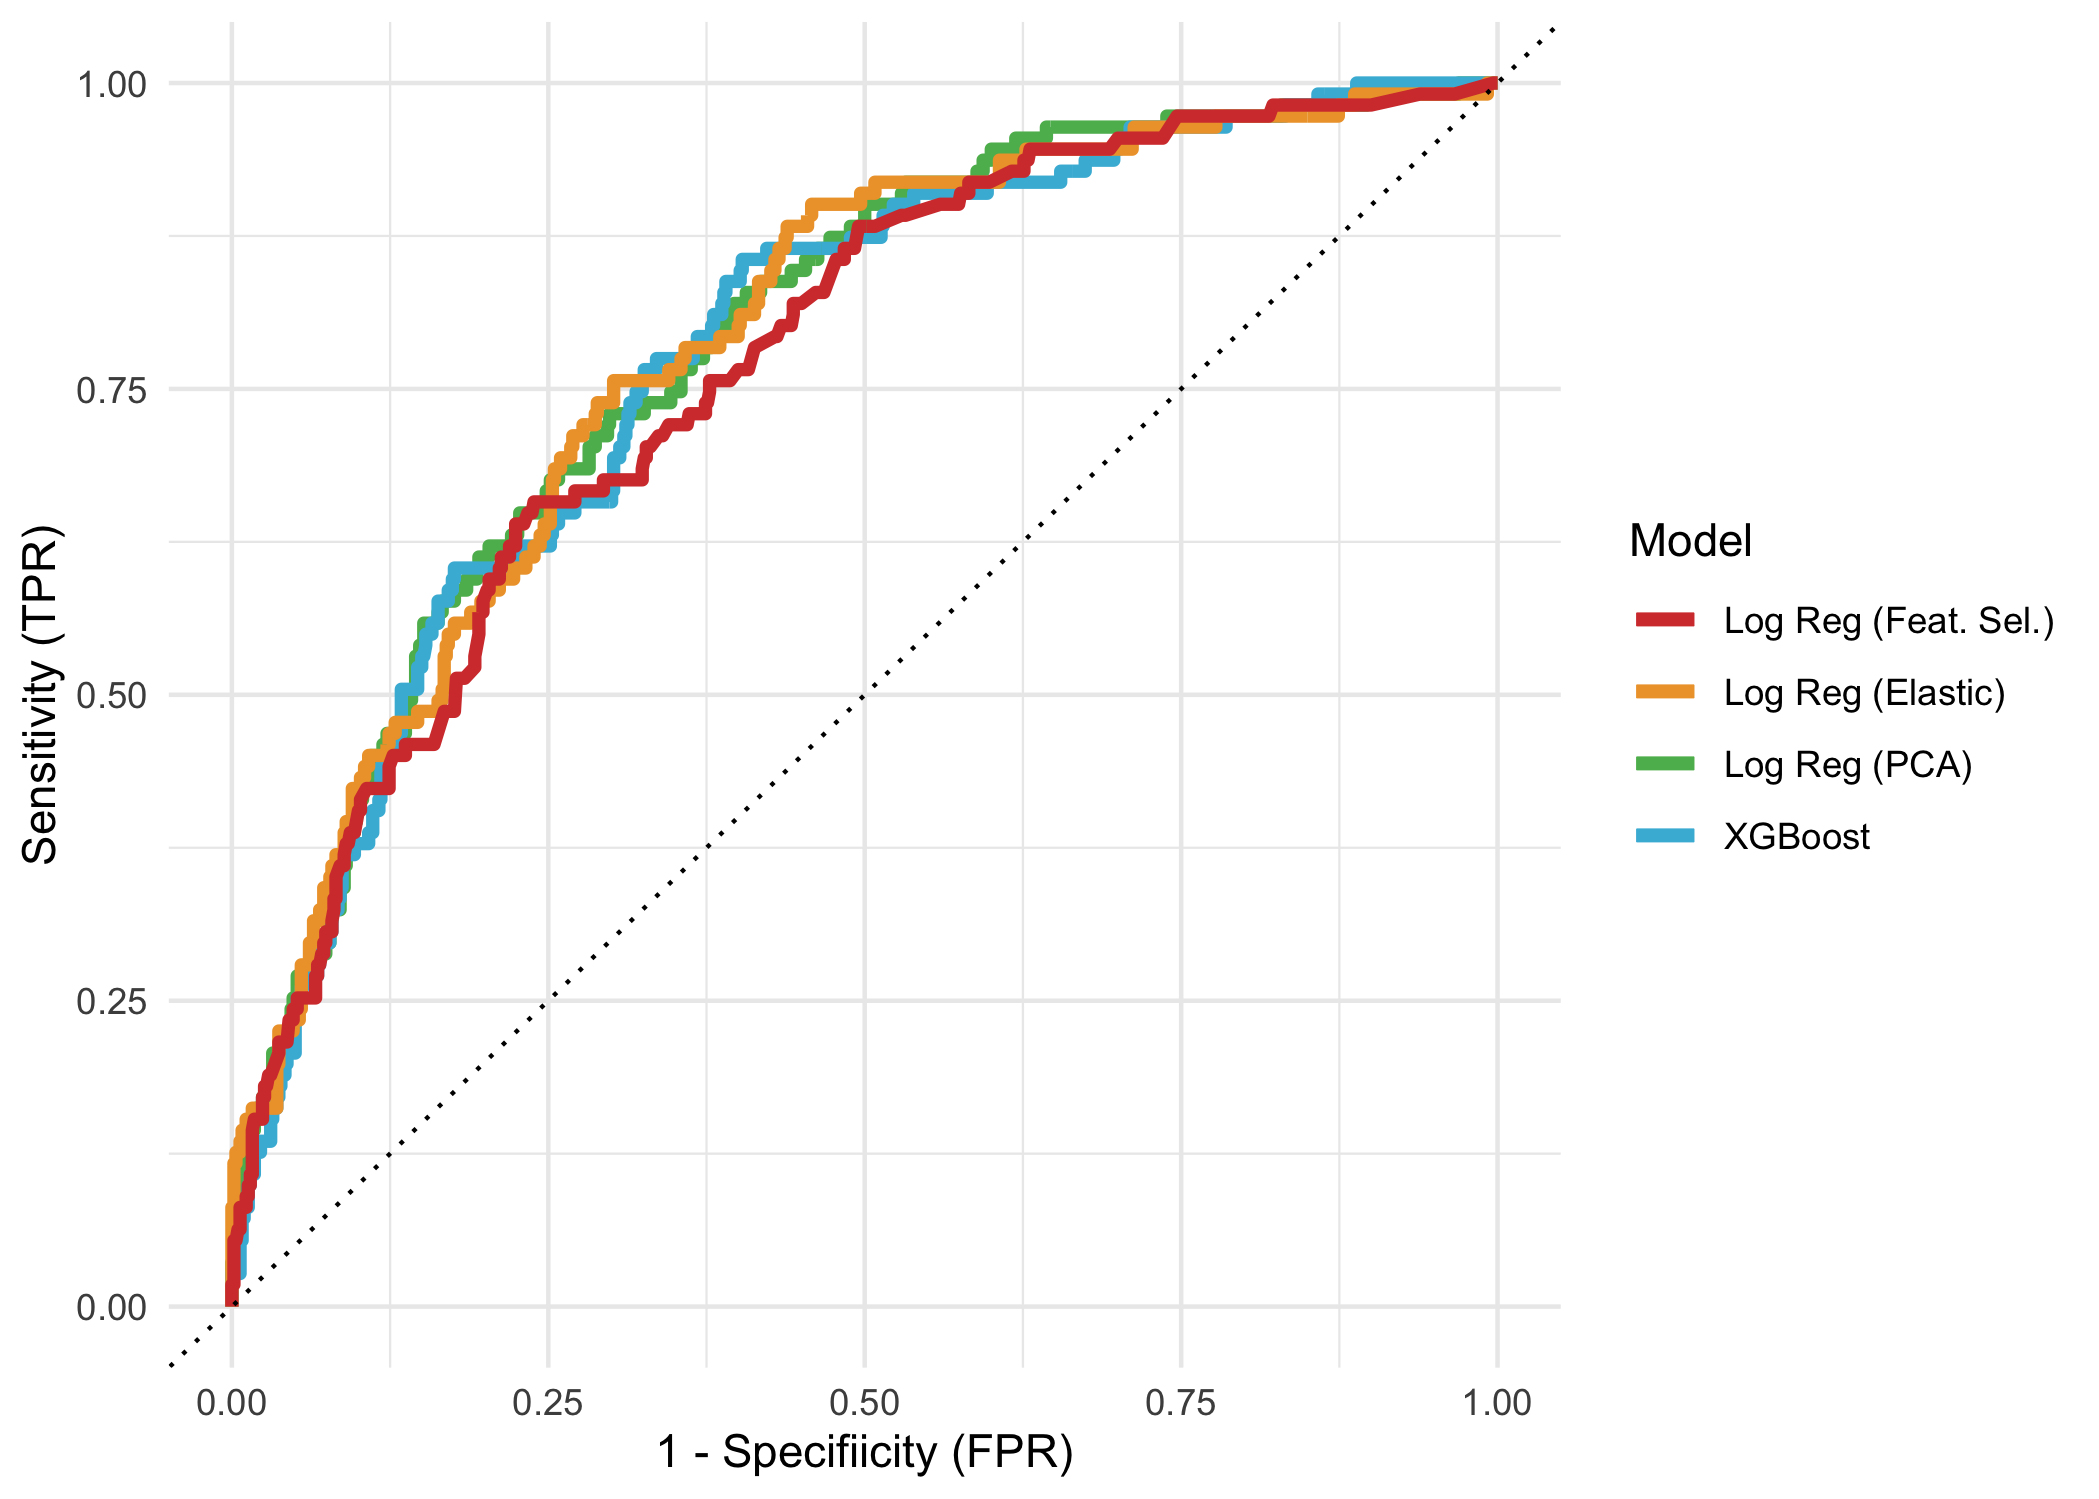
\includegraphics[height = 75mm, width=90mm]{results_roc.png}}
\hspace*{\fill}
\end{figure}


Although it is difficult to compare the models visually from this plot, it's clear from both the plot and the associated table of ROC-AUC scores that all four models demonstrated great predictive performance across the entire range of thresholds. They each exhibit an ability to successfully classify whether or not the patients have a 10-year risk of heart disease, and they appear to produce predictive results far better than a model that purely guesses (which is displayed by the black dotted line).

The associated ROC-AUCs from the table above also tell us that the logistic regression model using only feature selection distinguishes patients with and without a 10-year risk of heart disease the best across the whole range of thresholds. The logistic regression model using PCA for dimension reduction has a very close ROC-AUC score to the model using feature selection, and the difference in performance is so small that it may simply be a product of random variation when we initially split the test data. Interestingly, we can see that out of all the models, the XGBoost model seems to have had the worst testing performance across the entire range of thresholds.


\section*{Conclusion and Limitations}

In conclusion, we found several models that can successfully predict the 10-year risk of future heart disease. In fact, each model reduced the number of variables needed to predict the 10-year risk of heart disease. The subset of features from each model could help doctors and patients save countless time and money. Theoretically, a doctor could order specific tests related to the optimal variables in our model, and patients with lower income could save thousands of dollars with fewer tests. With so many different factors that can help predict the risk of 10-year heart disease, our results can give medical professionals a starting point. It is quite remarkable that we can obtain these results with machine learning and various forms of feature selection without a medical degree. Perhaps more advanced heart rate metrics and machines could provide better variables to predict the 10-year risk of heart disease. However, many of the features we used can be obtained in an annual physical. 

\newpage

\section*{Presentation Questions \& Answers}

\subsubsection*{Question \#1}

\textit{Why did you choose XGBoost over a Random Forest?}

\

Although the random forest model generally provides high accuracy, it is also prone to overfitting. Random forests unfortunately tend to overfit the training data when sampled data points are very similar to one another. Especially since we oversampled observations from the minority class in our training data, similar data points would have been seen frequently while training our model. Therefore, in order to prevent the chances of overfitting we decided to use XGBoost instead.

\

The XGBoost model uses an ensemble of weak learners (trees), and the depth of each tree is generally very short. These shorter trees often prevent overfitting and allow for a better generalization of the model. Therefore, we believed that the XBGoost's ability to counter overfitting would lead to a stronger predictive performance on our test set.

\

Additionally, we have both used random forest models in other projects throughout the MAS program and have never used XGBoost in a project before. We figured this project would be even more interesting if we modeled our data using XGBoost and officially learned how to tune the parameters in a practical setting.

\subsubsection*{Question \#2}

\textit{Which transformation method did you use before performing PCA?}

\

Since many of our predictor variables are in different units and had varying scales, we decided to \textbf{standardize} the data using the sample mean and standard deviation from the training set. That is, each original feature, $\mathbf{X}_i$, was centered and scaled such that:

$$\mathbf{X}_i' = \frac{\mathbf{X}_i-\bar{x}_i}{\hat{\sigma}_i}$$

where $\bar{x}_i$ and $\hat{\sigma}_i$ are the feature's associated sample mean and sample standard deviation found from the training set. We then performed our modeling using the transformed features, $\mathbf{X}_i'$, instead of the original features. Note that using the training set to estimate the mean and standard deviation was essential to reduce any possibility of data leakage (direct information about the testing set being shared with the training set). 

\newpage 

\printbibliography

\newpage

\section*{Appendix}

We include the code used for our exploratory data analysis below:

\

\lstinputlisting{eda.R}

\newpage

We include the code used for our modeling and testing below:

\

\lstinputlisting{modeling_and_results.R}


\end{document}